\documentclass[a4paper,10pt]{article}
%\documentclass[preview=false]{standalone}
% %%%% Define new conditional \ifplastex
% %%%% This ensure that the file complied normally without plasTeX.
\usepackage{plastex}

\usepackage{hyperref}

\ifplastex\else
\usepackage{standalone} %%%% Only load standalone when not in plasTeX
\standalonetrue
\usepackage{longtable} %%%% Only load longtable and ltcaption when not in plasTeX
\usepackage{ltcaption}
\fi

% Package for typesetting URLs
\usepackage{url}

% Package for including graphics.
\usepackage{graphicx}

\usepackage{multicol}

\usepackage{bsymb}

% Package for typesetting Event-B models
\usepackage[colour]{eventB}
%\usepackage{eventB-vhdl}

% Package for typesetting dates and times
\ifplastex
\newcommand{\EventBXTextManualDate}{January 20th, 2017}
\else
\usepackage{datetime}
\newdate{EventBXTextManualDate}{20}{1}{2017}
\fi
\newcommand{\EventBXTextFeatureVersion}{0.0.5}
\newcommand{\EventBXTextManualVersion}{0.0.1}

% Title
\title{EventB XText Front-end User Manual} 

% Author
\author{%
  Thai Son Hoang\\%
  ECS, University of Southampton\\%
  \texttt{\href{mailto:T.S.Hoang@ecs.soton.ac.uk}{T.S.Hoang at ecs dot soton dot ac dot uk}}%
}%


% Date
\date{%
  Version \EventBXTextManualVersion\\%
  (for feature version \EventBXTextFeatureVersion)\\
  \ifplastex
  \EventBXTextManualDate
  \else
  \displaydate{EventBXTextManualDate}%
  \fi
}

\begin{document}
\ifplastex%
\maketitle% Make title if in plasTeX mode.
\else%
 \ifstandalone%
 \maketitle % Make title if in standalone mode.
 \else%
 \fi%
\fi%

\section{CamilleX Overview}
\label{sec:overview}

The CamilleX provides new CamilleX constructs (XMachines and XContexts) which are text files which are automatically translated into the corresponding Rodin Event-B constructs (i.e., Machine and Context) accordingly.  Facility for translating from Rodin Event-B components to CamilleX components can be invoked manually. The overall process can be seen in Figure~\ref{fig:overview}.
\begin{figure}[!htbp]
  \centering
  \ifplastex
  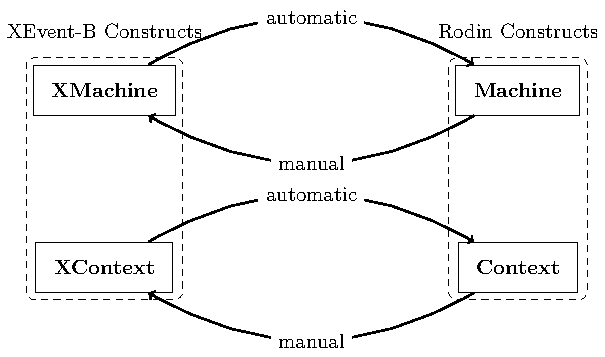
\includegraphics[width=512]{tikz-overview}
  \else
  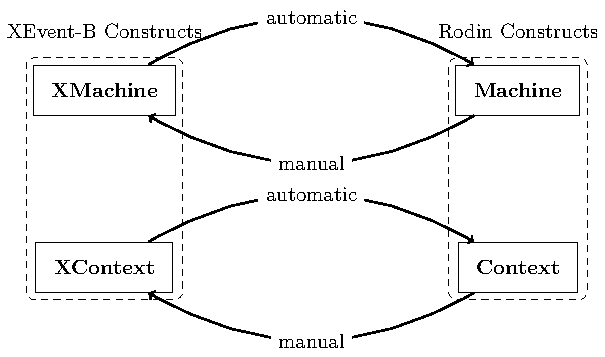
\includegraphics[width=0.9\textwidth]{tikz-overview}
  \fi
  \caption{Overview of CamilleX and Rodin Event-B Constructs}
  \label{fig:overview}
\end{figure}

%%% Local Variables:
%%% mode: latex
%%% TeX-master: "user_manual"
%%% End:


\section{Getting Started}
\label{sec:getting-started}

\subsection{Installation}
\label{sec:installation}

\subsubsection{Setup}
\label{sec:setup}

\begin{itemize}
\item Before installing the XEvent-B Front-end feature, you need to add the XText update site (\url{http://download.eclipse.org/modeling/tmf/xtext/updates/composite/releases/}) as an additional software site (see Figure~\ref{fig:xtext-updatesite}).
\begin{figure}[!htbp]
  \centering
  \ifplastex
  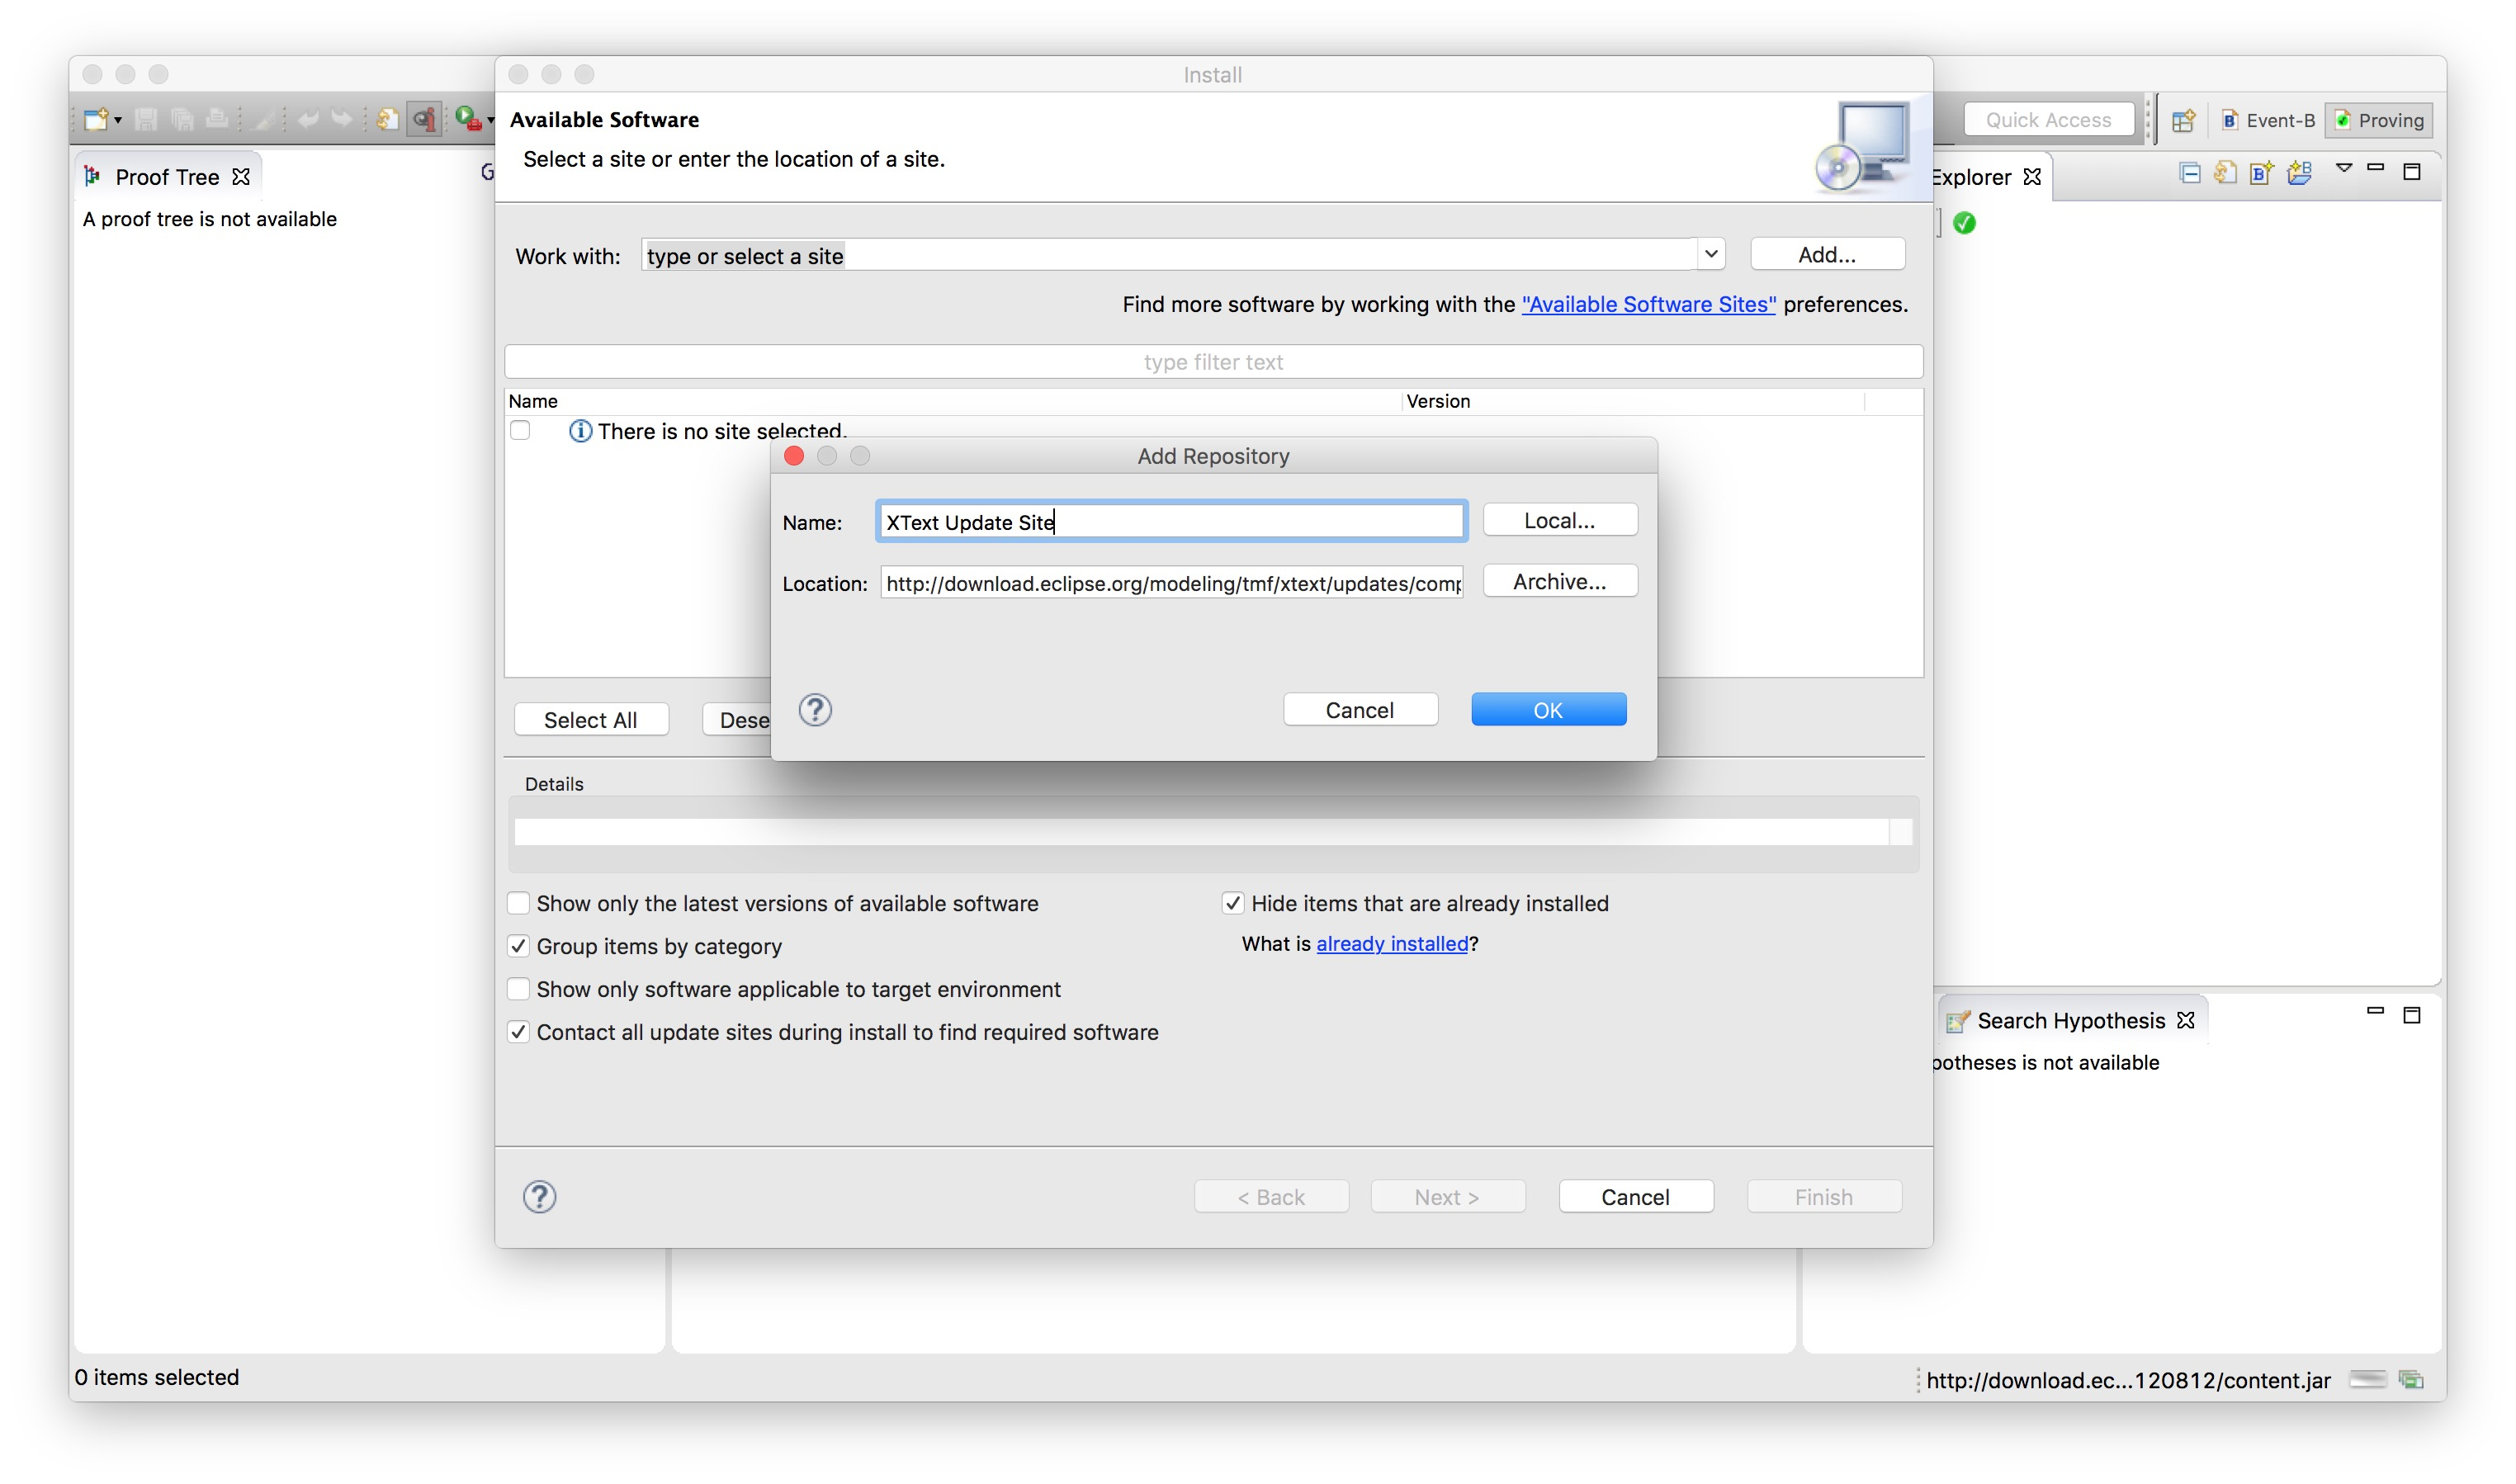
\includegraphics[width=512]{figures/XTextUpdateSite}
  \else
  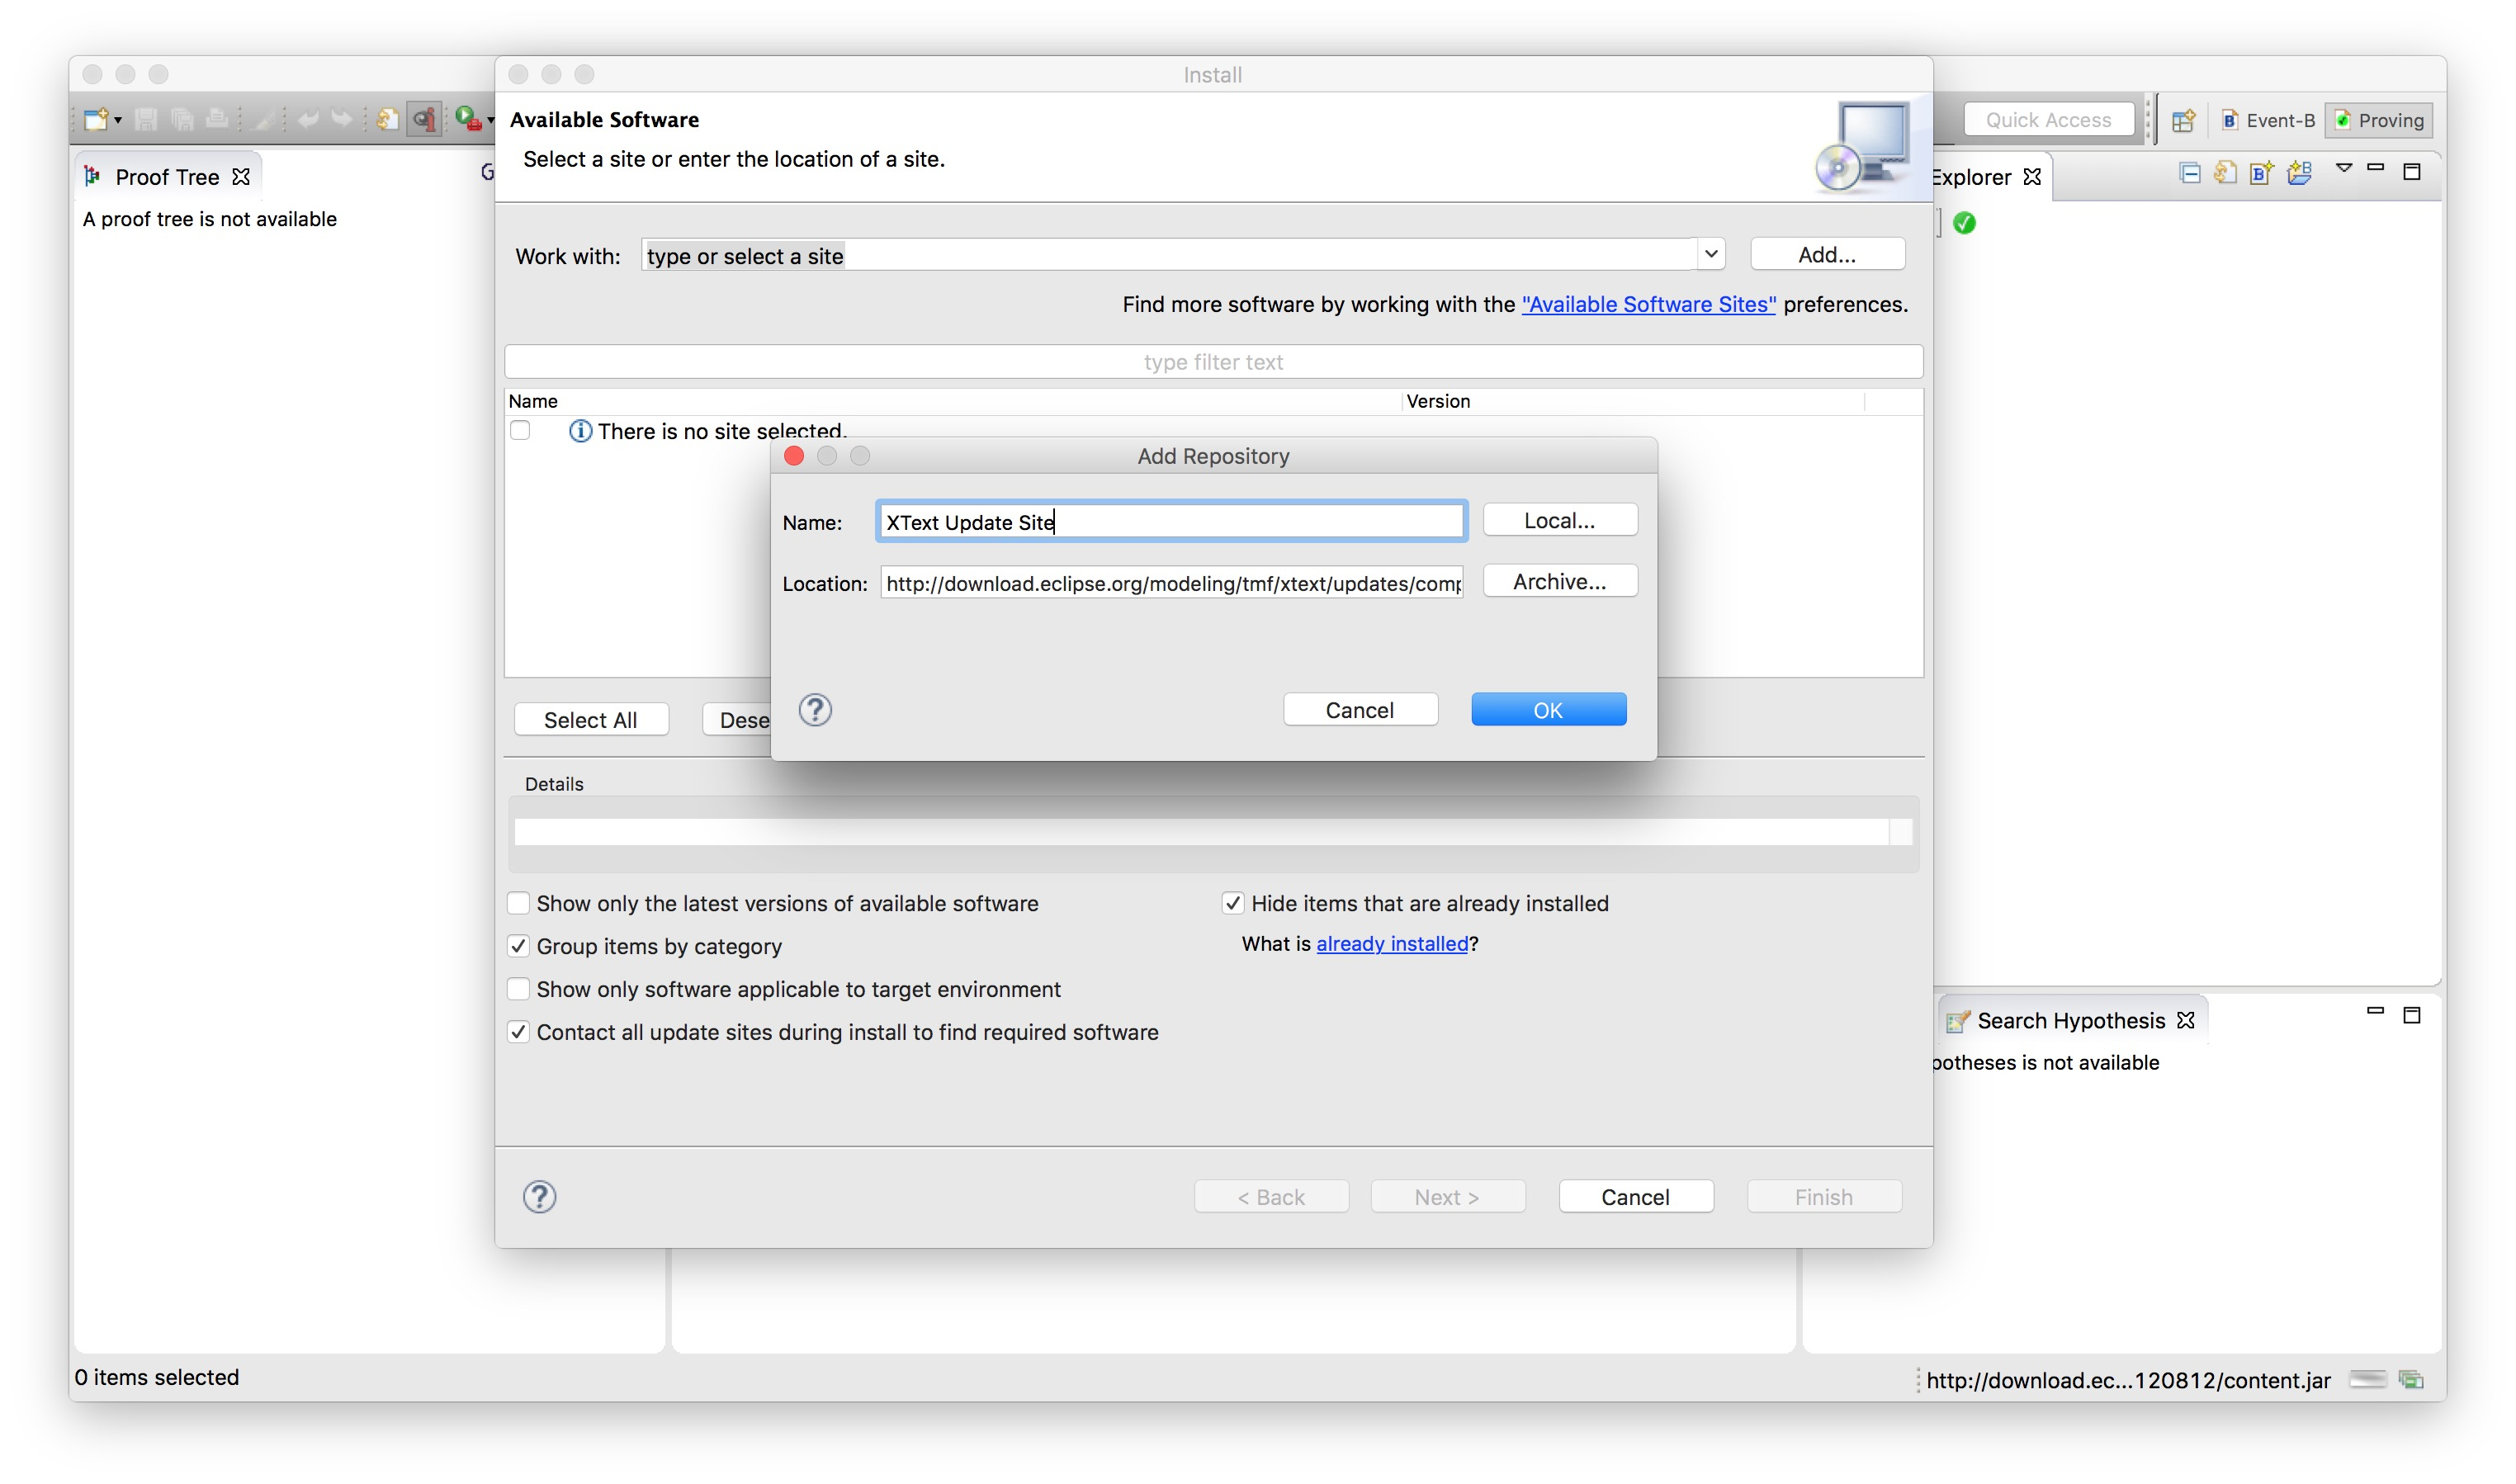
\includegraphics[width=0.9\textwidth]{figures/XTextUpdateSite}
  \fi
  \caption{Adding XText Update Site}
  \label{fig:xtext-updatesite}
\end{figure}


\item The XEvent-B front-end feature is available from the main Rodin update site (under ``Modelling Extensions'' category). There are two versions of the feature, \emph{eXtended Event-B (XEvent-B)} providing facilities for working with XEvent-B Front-end, and the \emph{eXtended Event-B (XEvent-B) (SDK)} is the feature including source code for software developers (see Figure~\ref{fig:EventBXText-installation}).
\begin{figure}[!htbp]
  \centering
  \ifplastex
  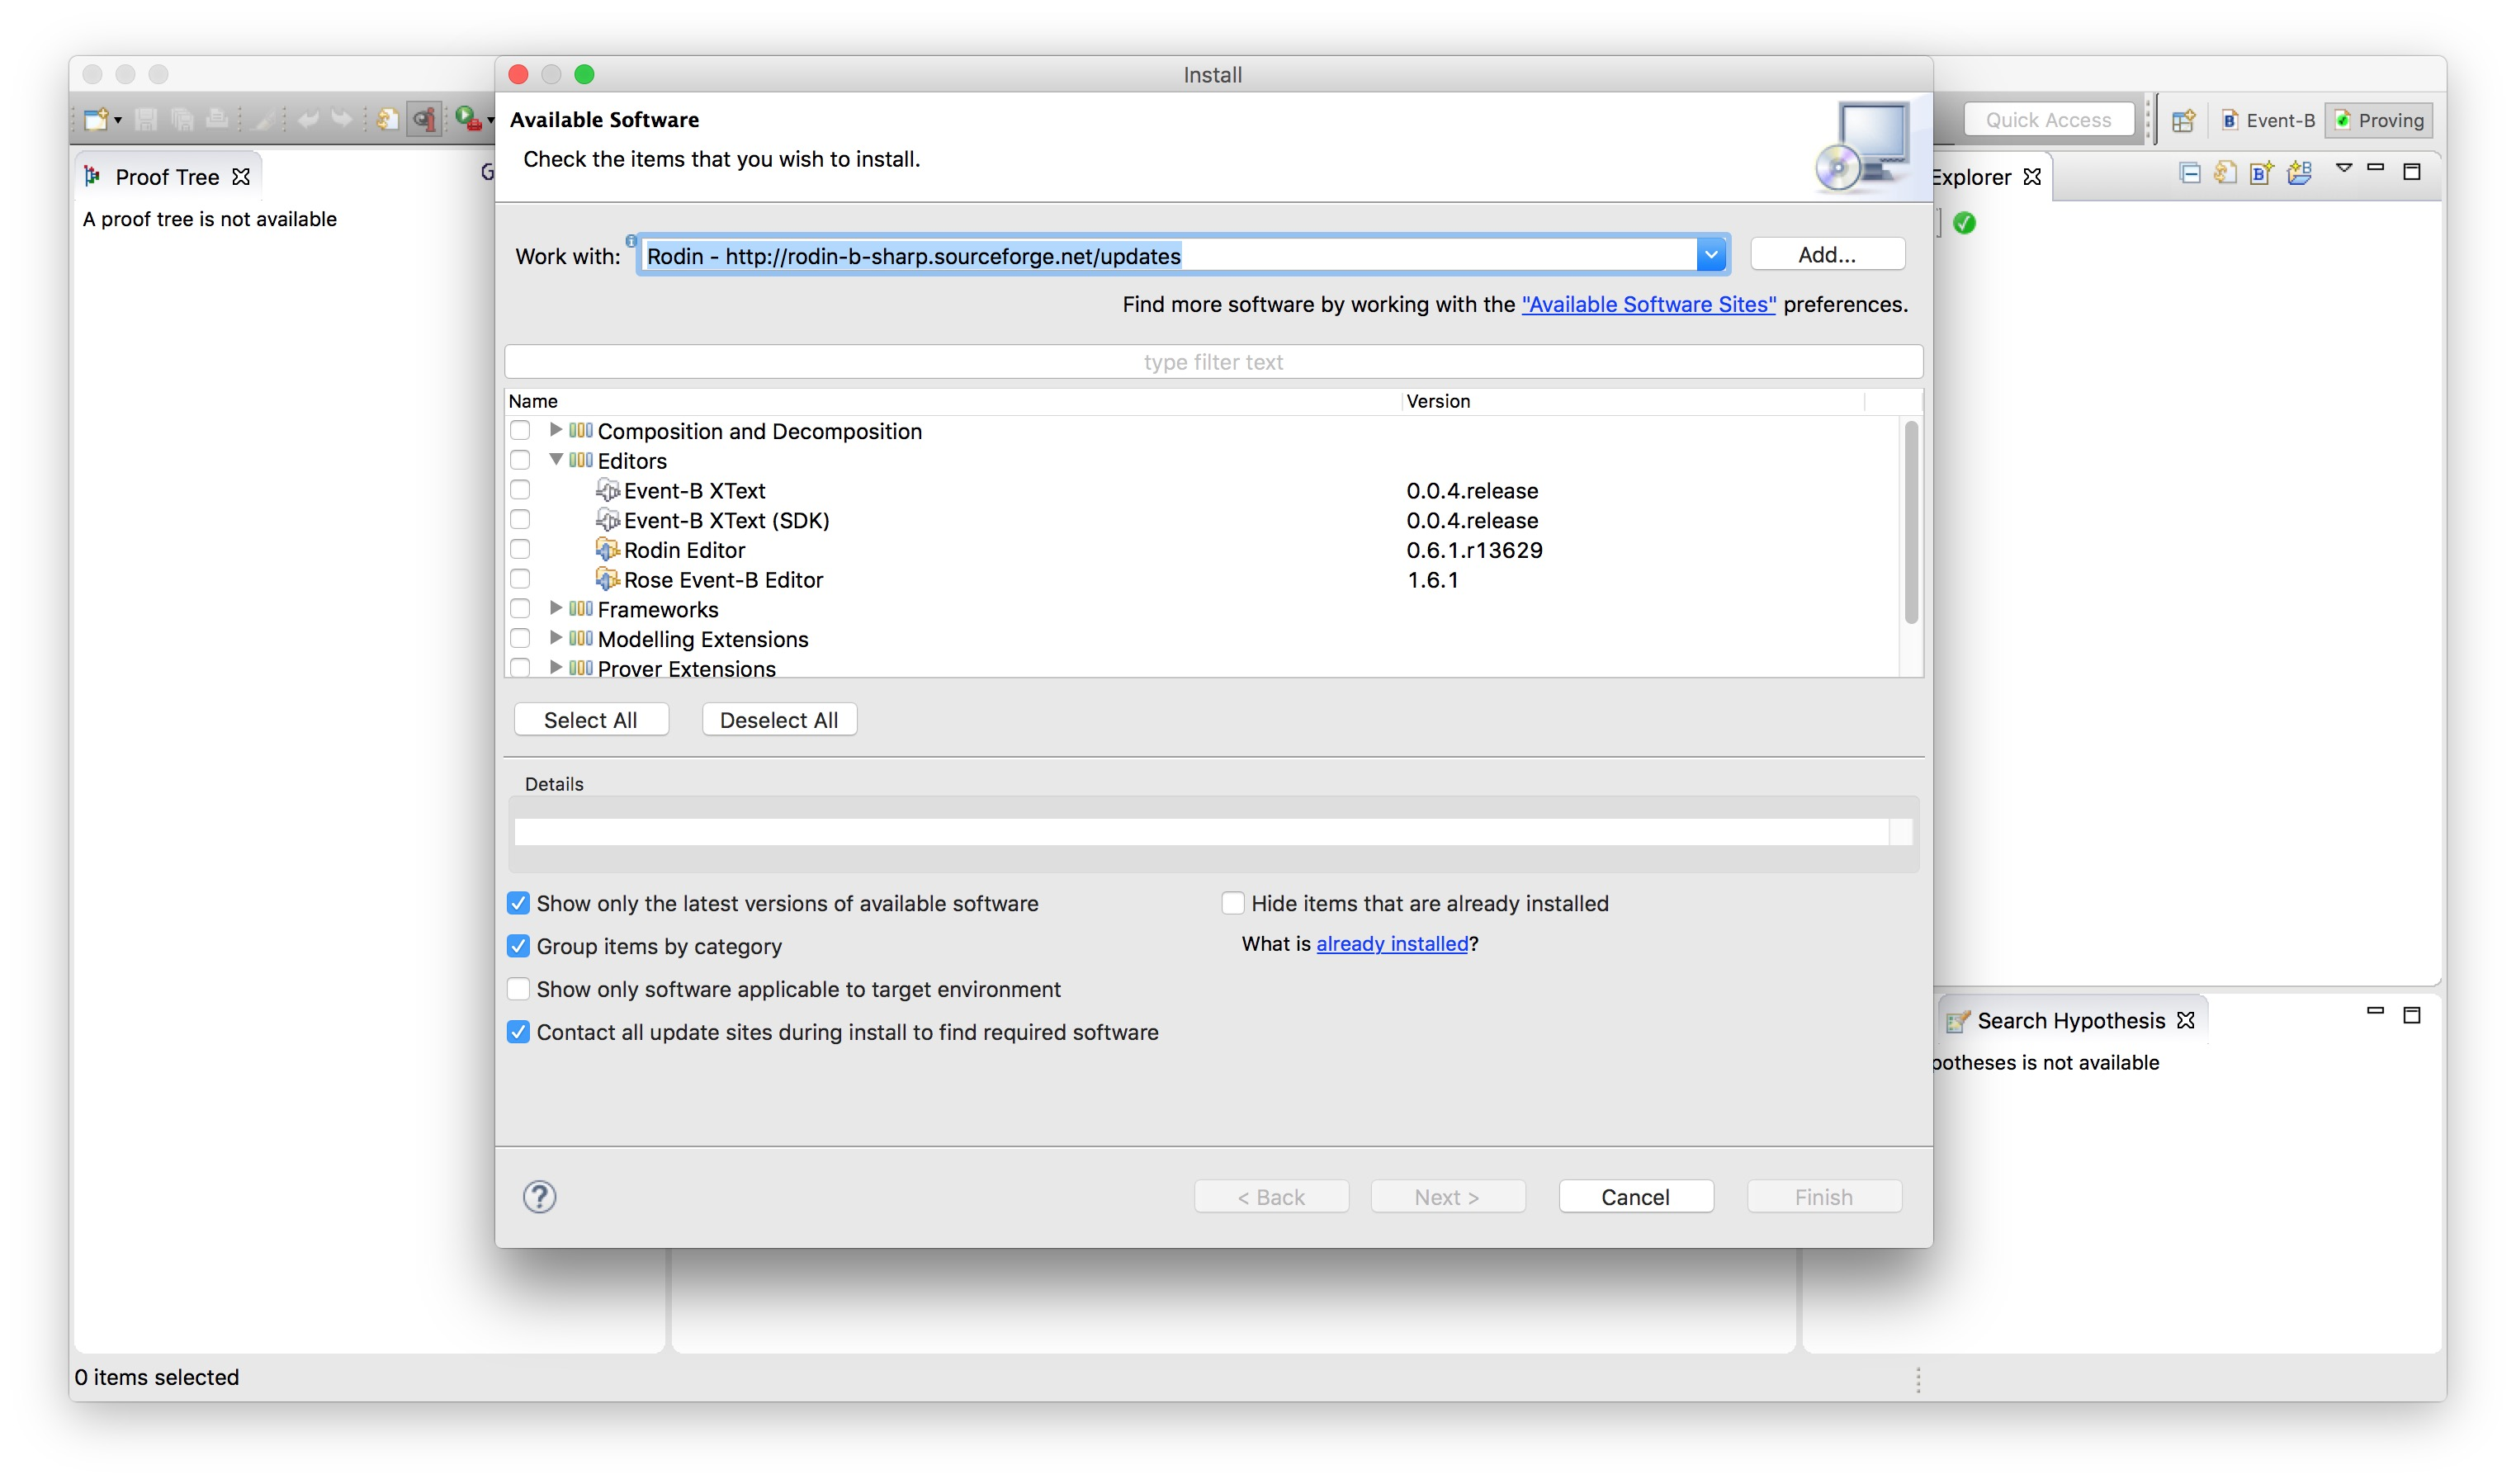
\includegraphics[width=512]{figures/EventBXTextInstallation}
  \else
  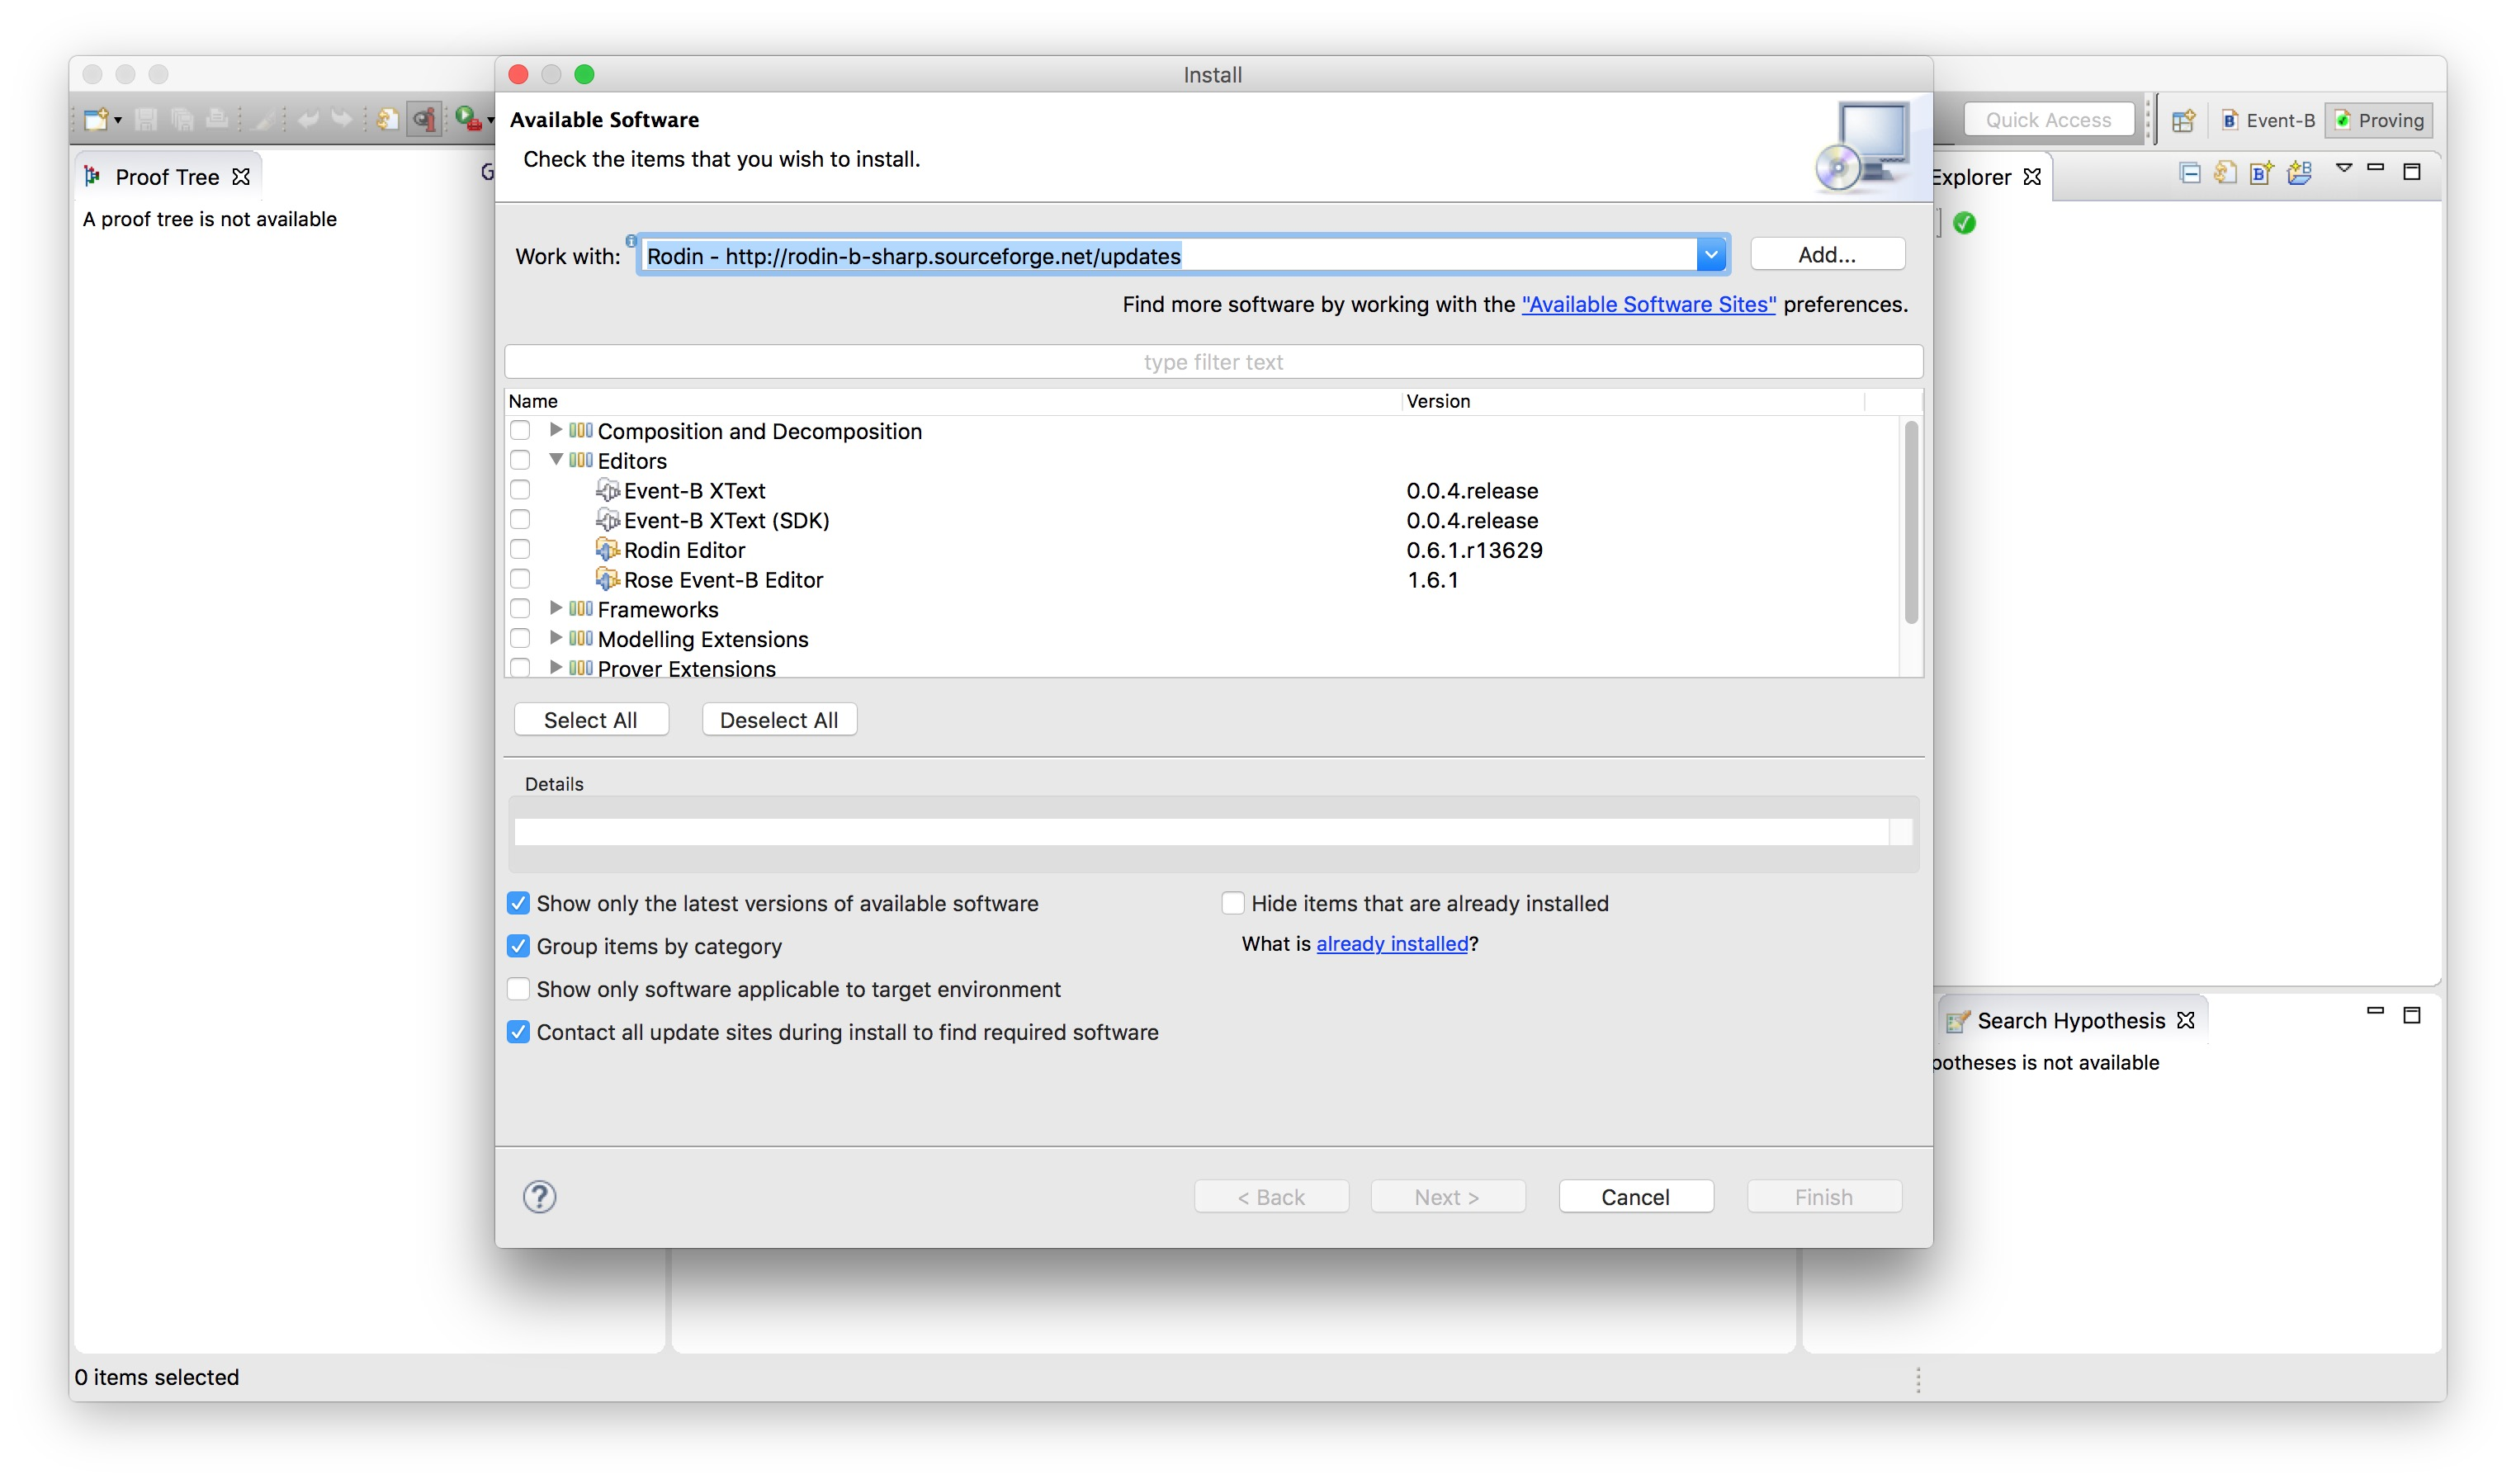
\includegraphics[width=0.9\textwidth]{figures/EventBXTextInstallation}
  \fi
  \caption{Adding XText Update Site}
  \label{fig:EventBXText-installation}
\end{figure}

\end{itemize}

\subsubsection{Release Notes}
\label{sec:release-notes}
\paragraph{0.0.7}
\begin{itemize}
\item XEvent-B Common (0.0.4): Enhancement (Issue \#11).
  \begin{itemize}
  \item Machines from different projects can now be included.

  \item  Machines are now included using qualified name defined as:
    \emph{projectName.machineName}
  \end{itemize}

\item  XEvent-B Documentations (0.0.7): Update documentation for 0.0.7 release.
\item  XEvent-B XContext (0.0.5): Changed dependency on XText to [2.12.0, 3.0.0).
\item  XEvent-B XContext IDE (0.0.4): Changed dependency on XText to [2.12.0, 3.0.0).
\item  XEvent-B XContext UI (0.0.4): Changed dependency on XText to [2.12.0, 3.0.0).
\item  XEvent-B XMachine (0.0.5):
  \begin{itemize}
  \item Changed dependency on XText to [2.12.0, 3.0.0).
  
  \item  Fixed Issue \#8: Comments are not parsed.
  
  \item  Fixed Issue \#10: Variants not translated: Fix is part of inclusion plug-in release 0.2.0.  
  
  \item  Flattened machines now have the included machine elements generated before the source machine.
  
  \item  Order of generating elements of multiple inclusions and/or instances is from last to first.
  
  \item  This update is part of inclusion plug-in release 0.2.0.
  \end{itemize}

\item  XEvent-B XMachine IDE (0.0.4): Changed dependency on XText to [2.12.0, 3.0.0).
\item  XEvent-B XMachine UI (0.0.4): 
  \begin{itemize}
  \item Changed dependency on XText to [2.12.0, 3.0.0).
  \item Regenerated from XEvent-B XMachine 0.0.5
  \end{itemize}
\end{itemize}

\paragraph{0.0.6}
\begin{itemize}
\item Renamed plug-ins and features to XEvent-B (instead of Event-B XText).
\item XEvent-B Branding (0.0.2): Renamed from Event-B XText Branding.
\item XEvent-B Documentations (0.0.2): Renamed from Event-B XText Documentations.
\item XEvent-B Cheatsheets (0.0.2): Renamed from Event-B XText Cheatsheets.
\item XEvent-B Common (0.0.3): Renamed from Event-B XText Common.
\item XEvent-B UI (0.0.2): Renamed from Event-B XText UI.
\item XEvent-B XContext (0.0.4): Renamed from Event-B XText Context.
\item XEvent-B XContext IDE (0.0.3): Renamed from Event-B XText Context IDE.
\item XEvent-B XContext UI (0.0.3): Renamed from Event-B Context UI.
\item XEvent-B XMachine (0.0.4): Renamed from Event-B XText Machine.
	\begin{itemize}
		\item Support Machine Inclusion and Event Synchronisation.
	\end{itemize}	
\item XEvent-B XMachine IDE (0.0.3): Renamed from Event-B XText Machine IDE.
\item XEvent-B XMachine UI (0.0.3): Renamed from Event-B XText Machine UI.
\end{itemize}

\paragraph{0.0.5}
\begin{itemize}
\item Event-B XText Documentations (0.0.1): Documentation plug-in (Initial version).
\end{itemize}

\paragraph{0.0.4}
\begin{itemize}
\item Updated plug-in dependency for the feature
\end{itemize}

\paragraph{0.0.3}
\begin{itemize}
\item Event-B XText Context (0.0.3):
  \begin{itemize}
  \item Issue \#3: Single-line comment after the element, multi-line comment before
    the element
  \end{itemize}

\item Event-B XText Context IDE (0.0.2): Regenerated
 
\item Event-B XText ContextUI IDE (0.0.2): Regenerated

\item Event-B XText Machine (0.0.3):
  \begin{itemize}
  \item Issue \#3: Single-line comment after the element, multi-line comment before
    the element.

  \item Issue \#5: Event terminator using 'end' keyword instead of ';'
  \end{itemize}

\item Event-B XText Machine IDE (0.0.2) Regenerated
  
\item Event-B XText Machine UI IDE (0.0.2) Regenerated
\end{itemize}


\paragraph{0.0.2}
\begin{itemize}
\item Event-B XText Common (0.0.2):
  \begin{itemize}
  \item Added transient value service for XContext and XMachine.
  \end{itemize}

\item Event-B XText Context (0.0.2):
  \begin{itemize}
  \item Added formatter (used for auto-indentation).
  \end{itemize}

\item Event-B XText Machine (0.0.2):
  \begin{itemize}
  \item Added formatter (used for auto-indentation).
  \end{itemize}

\item Event-B XText UI (0.0.1): Initial version
  \begin{itemize}
  \item Added context menu for converting machines and contexts to XText.
  \end{itemize}
\end{itemize}

\paragraph{0.0.1} Initial version contains the following plug-ins:
\begin{itemize}
\item Event-B XText Branding (0.0.1) Initial version: Branding information

\item Event-B XText Common (0.0.1) Initial version: Common facilities

\item Event-B XText Context (0.0.1) Initial version: Core support for Event-B contexts

\item Event-B XText Context IDE (0.0.1) Initial version: IDE for Event-B contexts

\item Event-B XText Context UI (0.0.1) Initial version: UI for Event-B contexts

\item Event-B XText Machine (0.0.1) Initial version: Core support for Event-B machines

\item Event-B XText Machine IDE (0.0.1) Initial version: IDE for Event-B machines

\item Event-B XText Machine UI (0.0.1) Initial version: UI for Event-B machines
\end{itemize}

\subsubsection{IMPORTANT}
\label{sec:important}

\begin{itemize}
\item Currently, XEvent-B front-end \textbf{not only} supports ``standard'' Event-B machines and contexts, but also supports ``\emph{Machine Inclusion}'' and ``\emph{Event Synchronisation}''.
\item Since the XContexts and XMachines are compiled to the Rodin files, the corresponding Rodin contexts and machines will be \textbf{OVER-WRITTEN}. Any changes in the Rodin files will not be lost.

\item \textbf{DO NOT USE} the XEvent-B Front-end if you use modelling plug-ins such as \emph{iUML-B} state-machines and class-diagrams, as the additional modelling elements will be over-written.

\item Windows users \textbf{must} change the workspace text file encoding to \textbf{UTF-8}. This can be updated under the Rodin Preferences: General/Workspace then in the ``\emph{Text file encoding}'' section, select Other: UTF-8.

\end{itemize}

\subsubsection{Known Issues}
\label{sec:known-issues}

\begin{itemize}
\item Converting to XText: Currently, the ``extended'' attribute of events are not serialised.

\item Machine Inclusion: 
\begin{itemize}
	\item Including the \textbf{same} machine to both the abstract and its refining machine can result in the repetition of invariants.
\end{itemize}

\end{itemize}

\subsubsection{Configuration}
\label{sec:configuration}

\paragraph{Event-B Explorer}
By default, XContext files (extension .bucx) and XMachine files (extension .bumx) are not displayed in the \emph{Event-B Explorer}. To enable this, select \emph{Customize view} for \emph{Event-B Explorer} and uncheck the option \emph{All files and folders}.

\subsection{Basic Tutorial}
\label{sec:basic-tutorial}

This tutorial provides a step-by-step walk-through working with XEvent-B constructs. This tutorial also available as Cheatsheets with the Rodin Platform (\texttt{Help/Cheat Sheets/Event-B XText Cheatsheets/Event-B XText Basic Tutorial}).

\subsubsection{Task 1. Customise the Event-B Explorer}
\textbf{Introduction}
The purpose of this task is to customise the Event-B Explorer so that XEvent-B constructs are visible.
\begin{description}
\item[Step 1. Disable the filter on ``All files and folders''] Select ``Customize View'' of Event-B Explorer View. Make sure that ``All files and folders'' from the dialog is \textbf{Unchecked}.
\end{description}

\textbf{Conclusion} Since the filter on ``All files and folders'' is now disabled, there might be other files and folders than XEvent-B constructs will also be visible in the Event-B Explorer.

\subsubsection{Task 2. Create an Event-B Project}\label{CreateProject}
\textbf{Introduction} The purpose of this task is to create an Event-B project for the XEvent-B constructs. 
\begin{description}
\item[Step 1. Create a new Event-B Project] Create a new Event-B Project named ``Club'' using the \emph{New Event-B Project} wizard (see Figure~\ref{fig:CreateProject}).
\begin{figure}[!htbp]
  \centering
  \ifplastex
  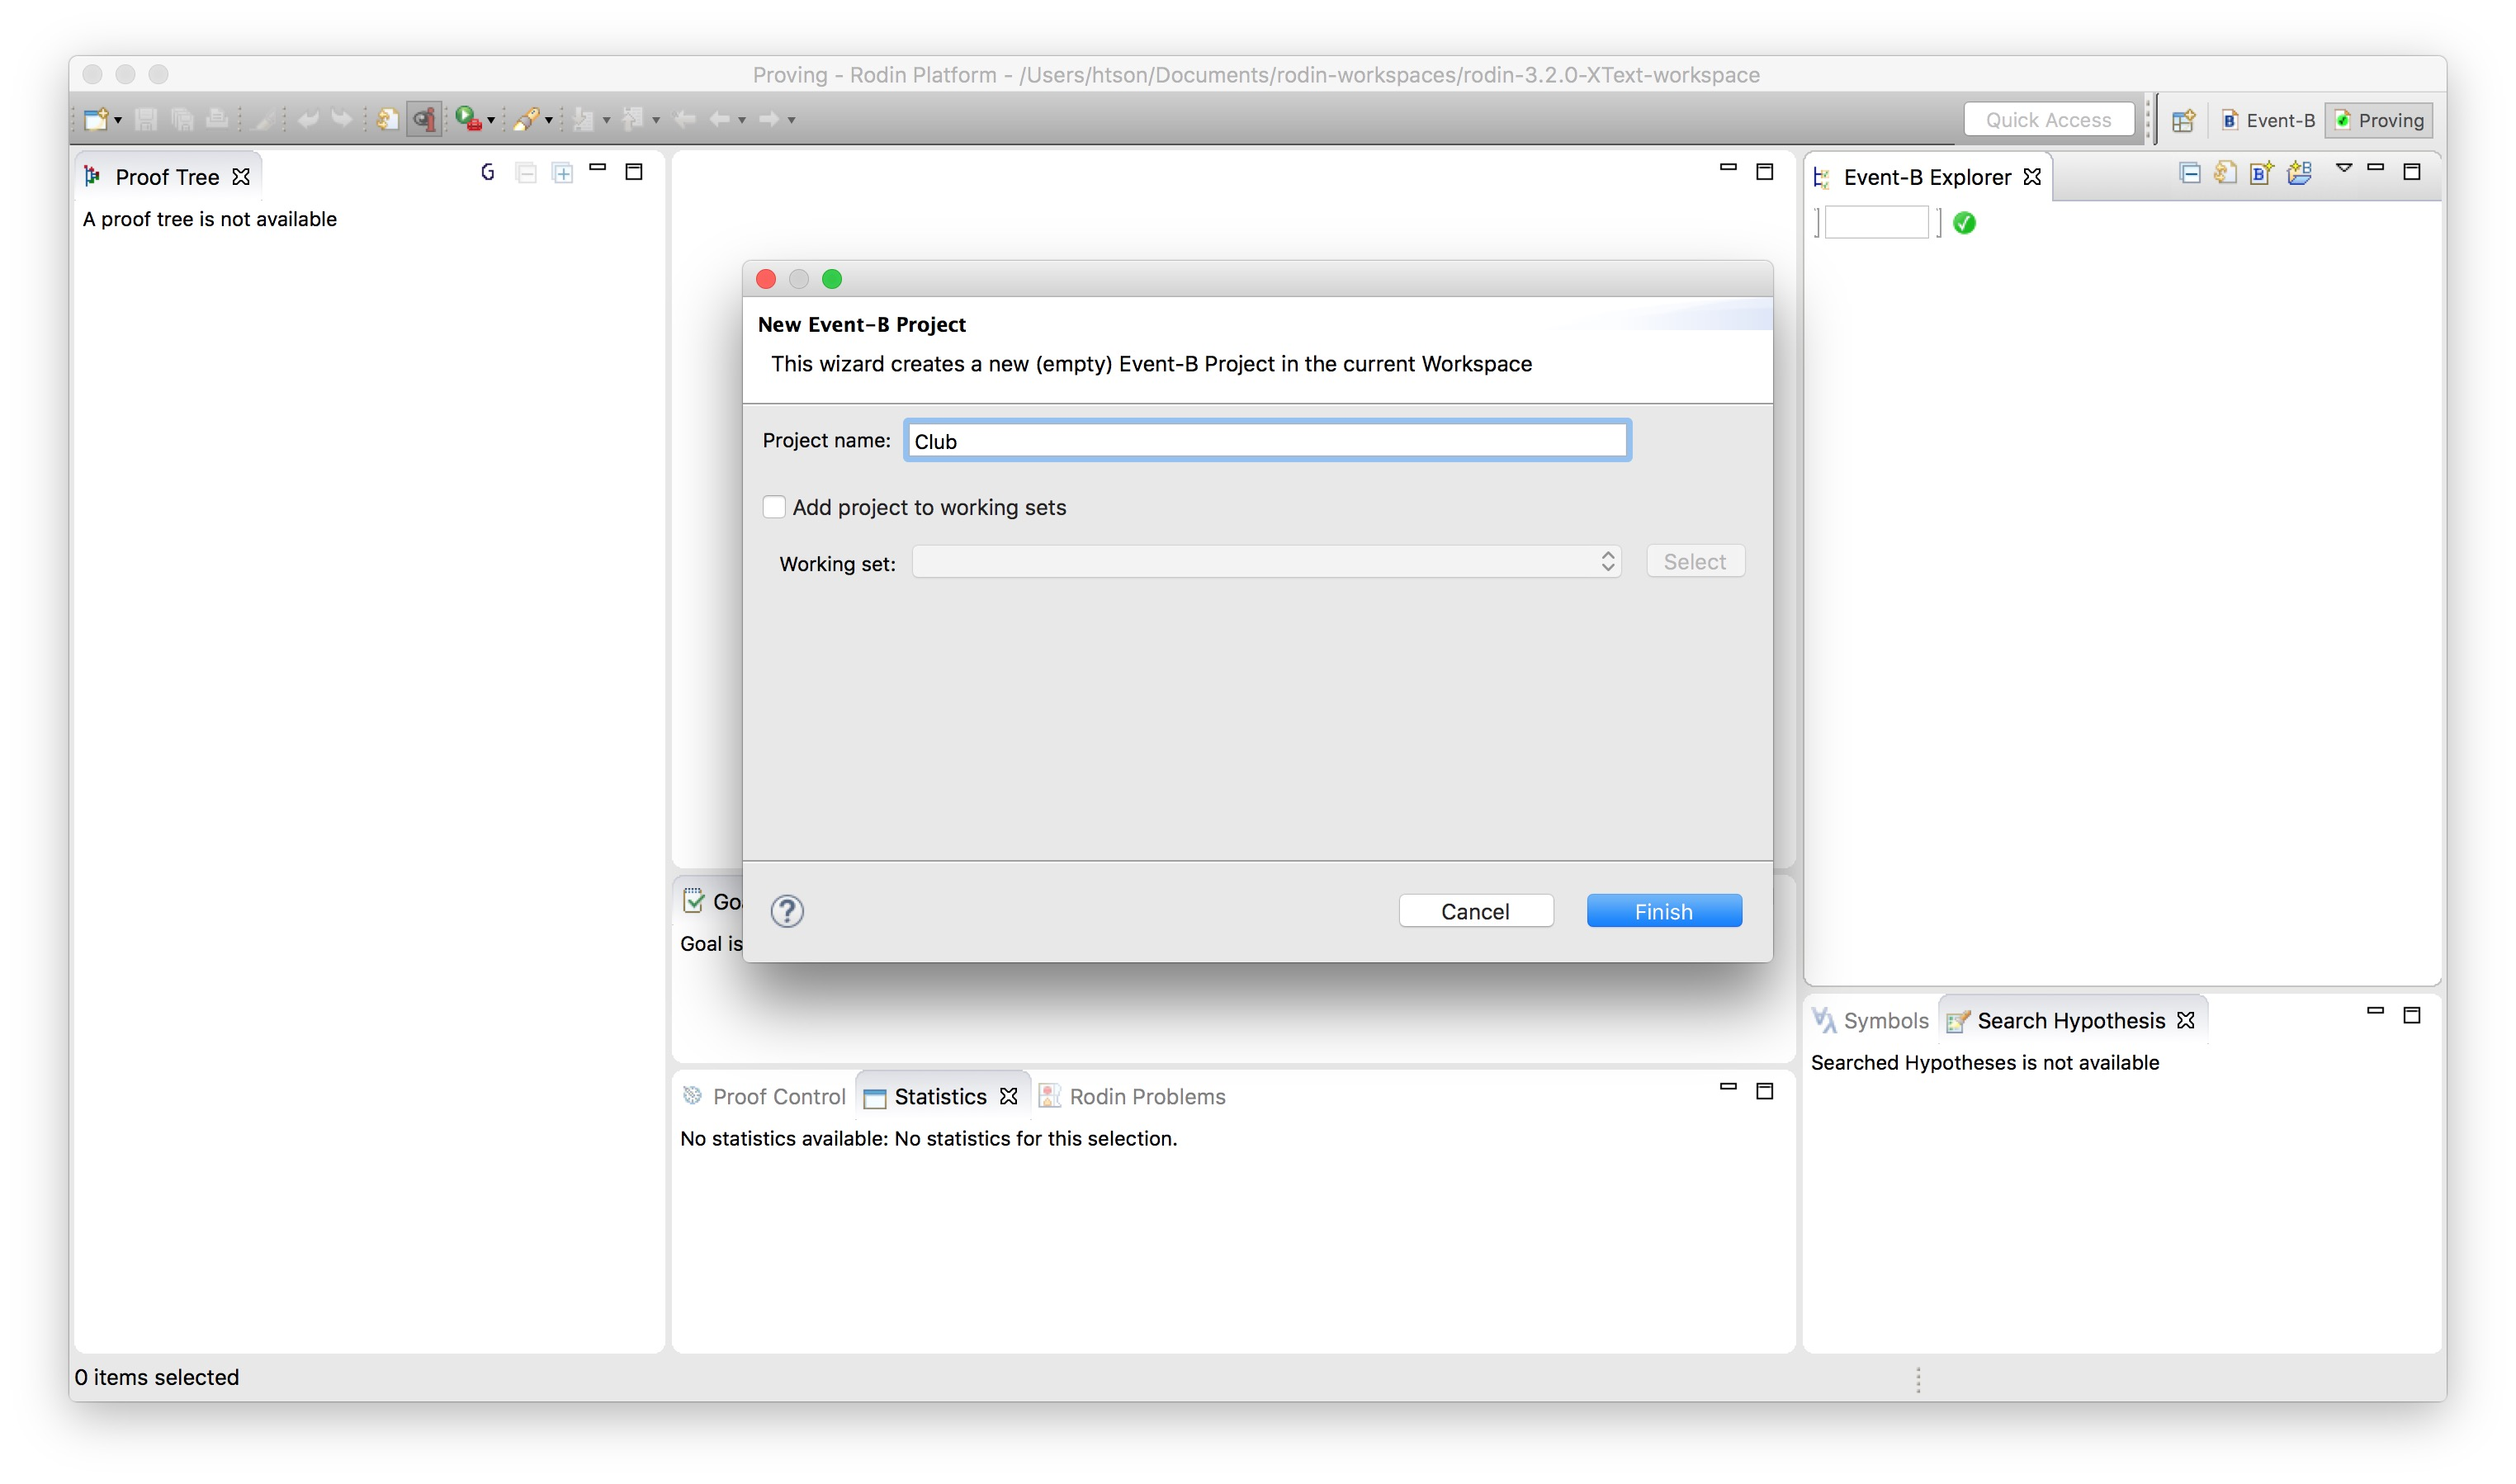
\includegraphics[width=512]{figures/CreateProject}
  \else
  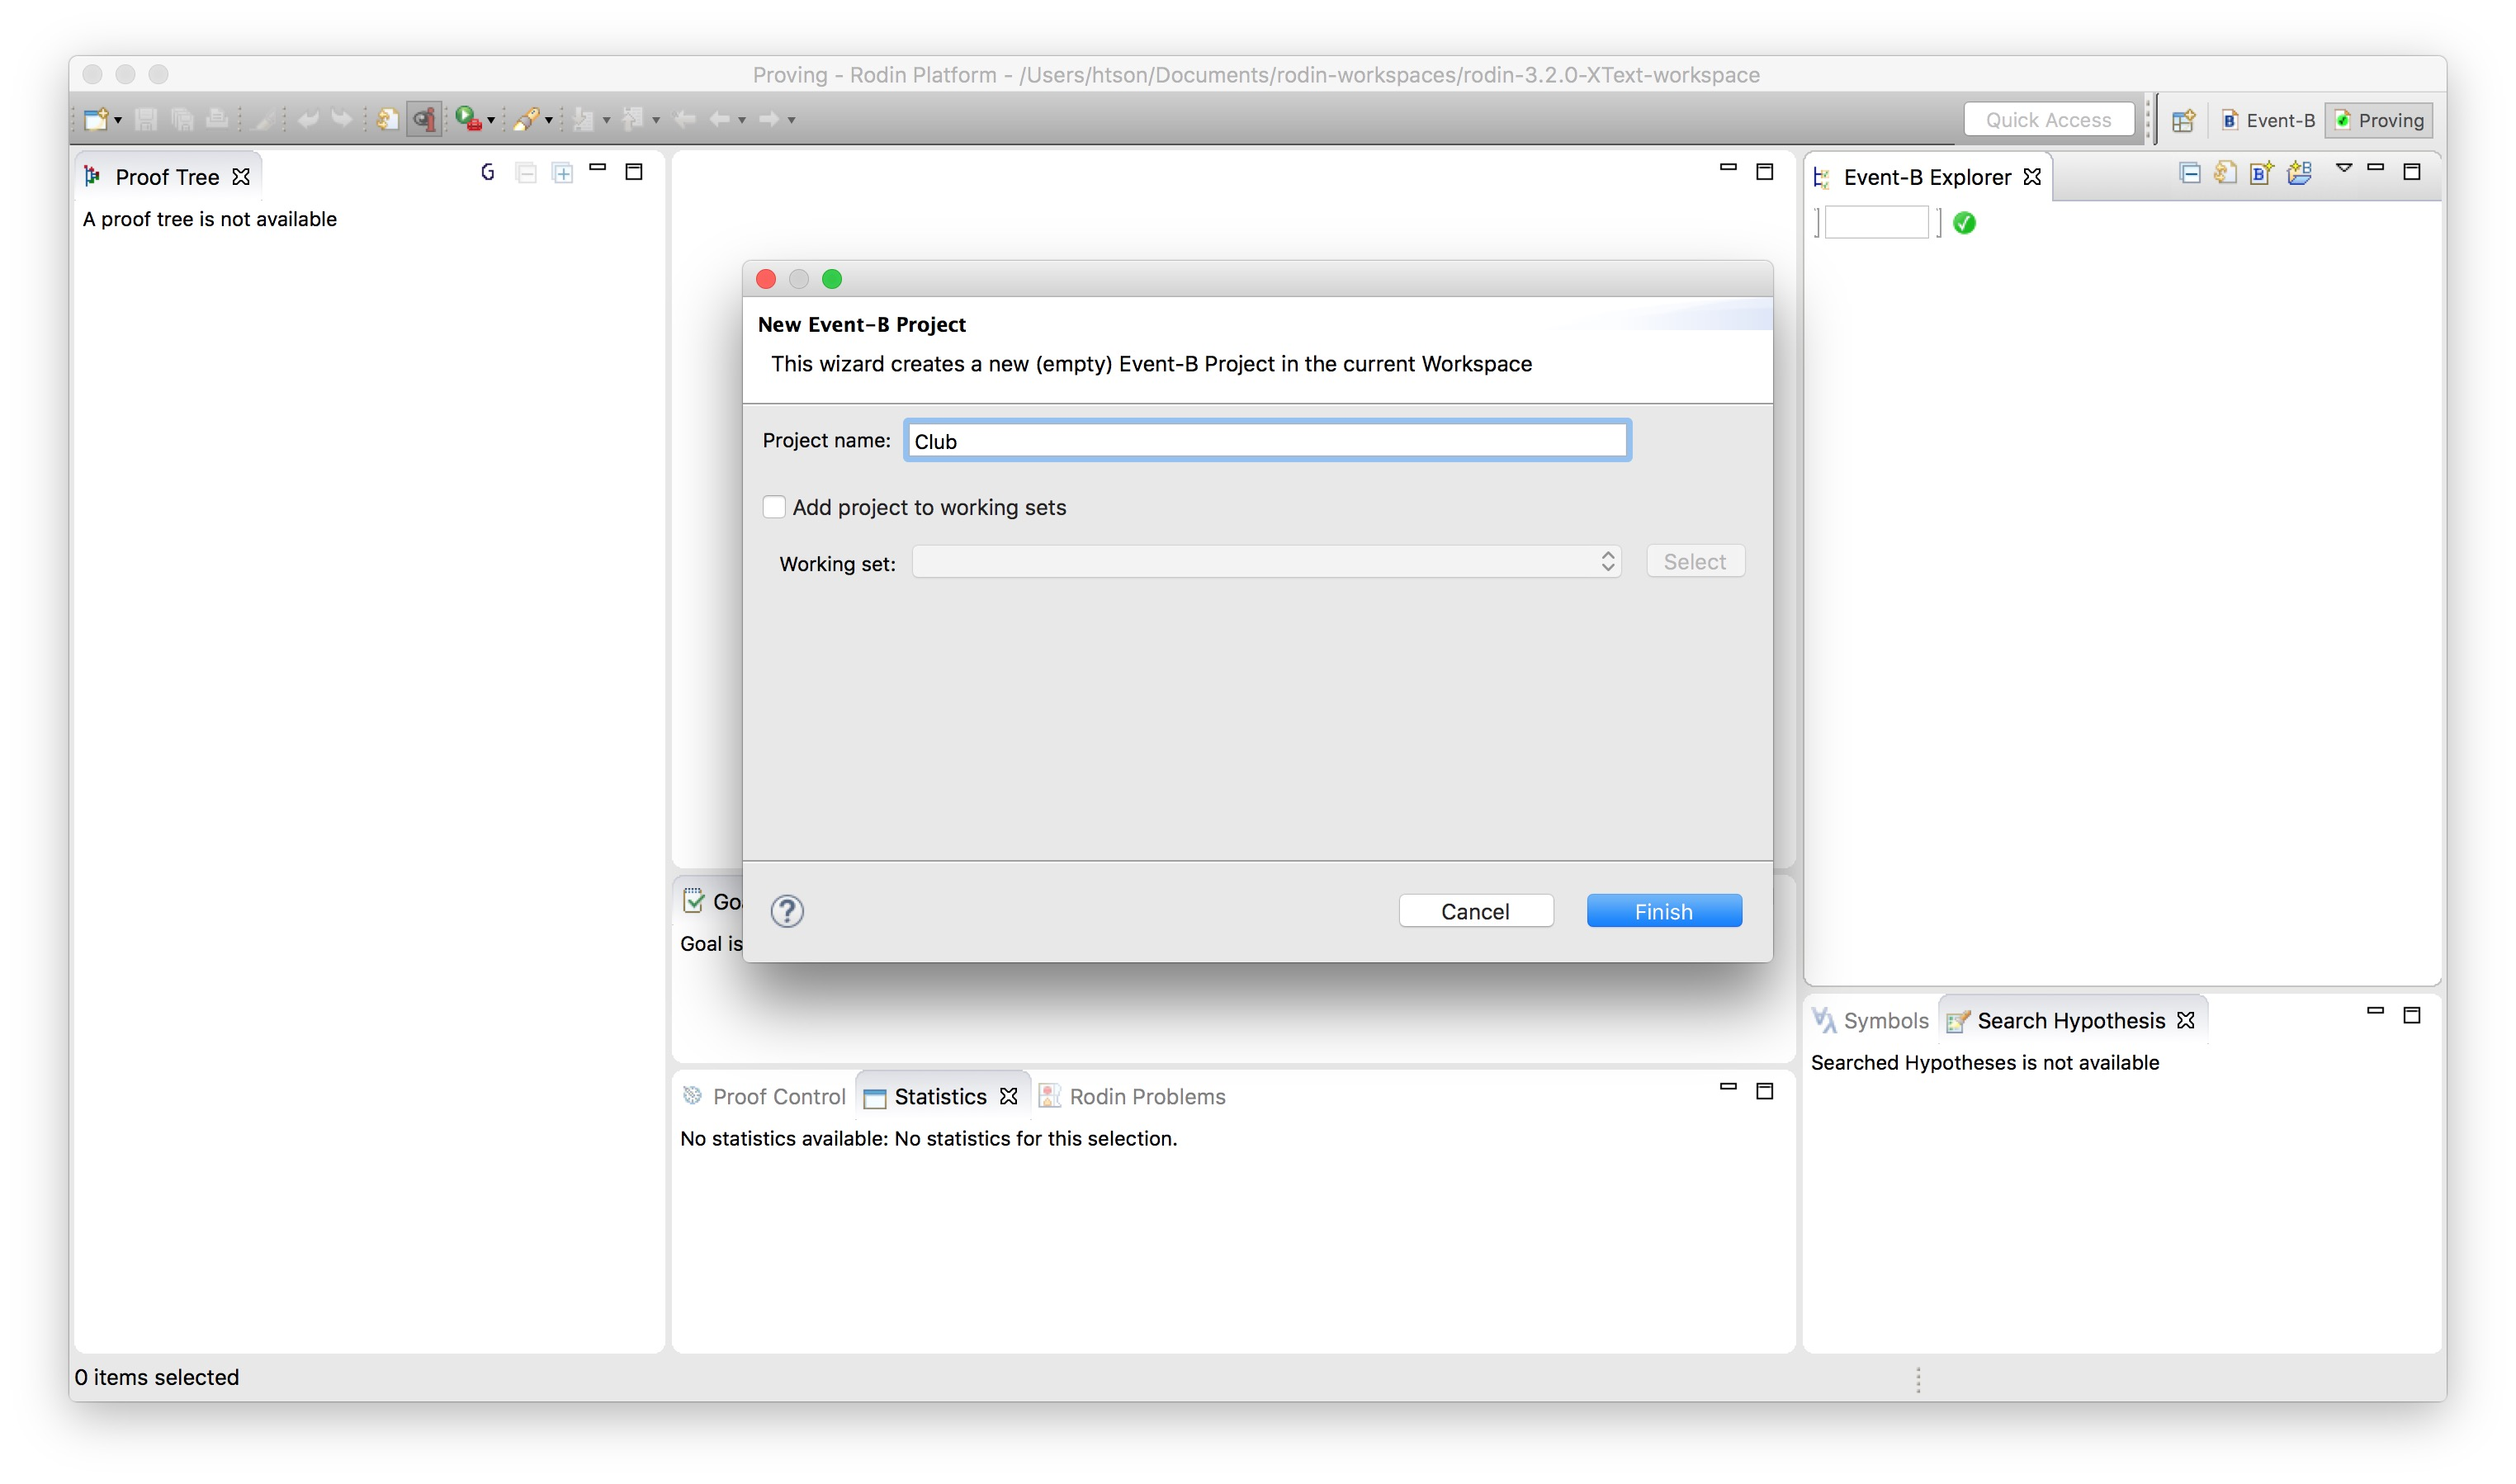
\includegraphics[width=0.9\textwidth]{figures/CreateProject}
  \fi
  \caption{Create Event-B Project called ``Club''}
  \label{fig:CreateProject}
\end{figure}

\end{description}
\textbf{Conclusion} By now, the project ``Club'' should be visible in the Event-B Explorer.


\subsubsection{Task 3. Create a simple XContext coursesCtx.bucx}\label{Sec:SimpleContext}
\textbf{Introduction} The purpose of this task is to create a simple XContext within the newly created project.
\begin{description}
\item[Step 1. Create a new XContext coursesCtx.bucx] Create a new XContext named ``coursesCtx.bucx'' using the \emph{New File wizard} (see Figure~\ref{fig:CreateCoursesCtx}).
         \textbf{Important}: A pop-up dialog will be displayed asking to convert the ``Club''
         project to XText project, please answer \textbf{Yes} (see Figure~\ref{fig:ConvertToXText}).
\begin{figure}[!htbp]
  \centering
  \ifplastex
  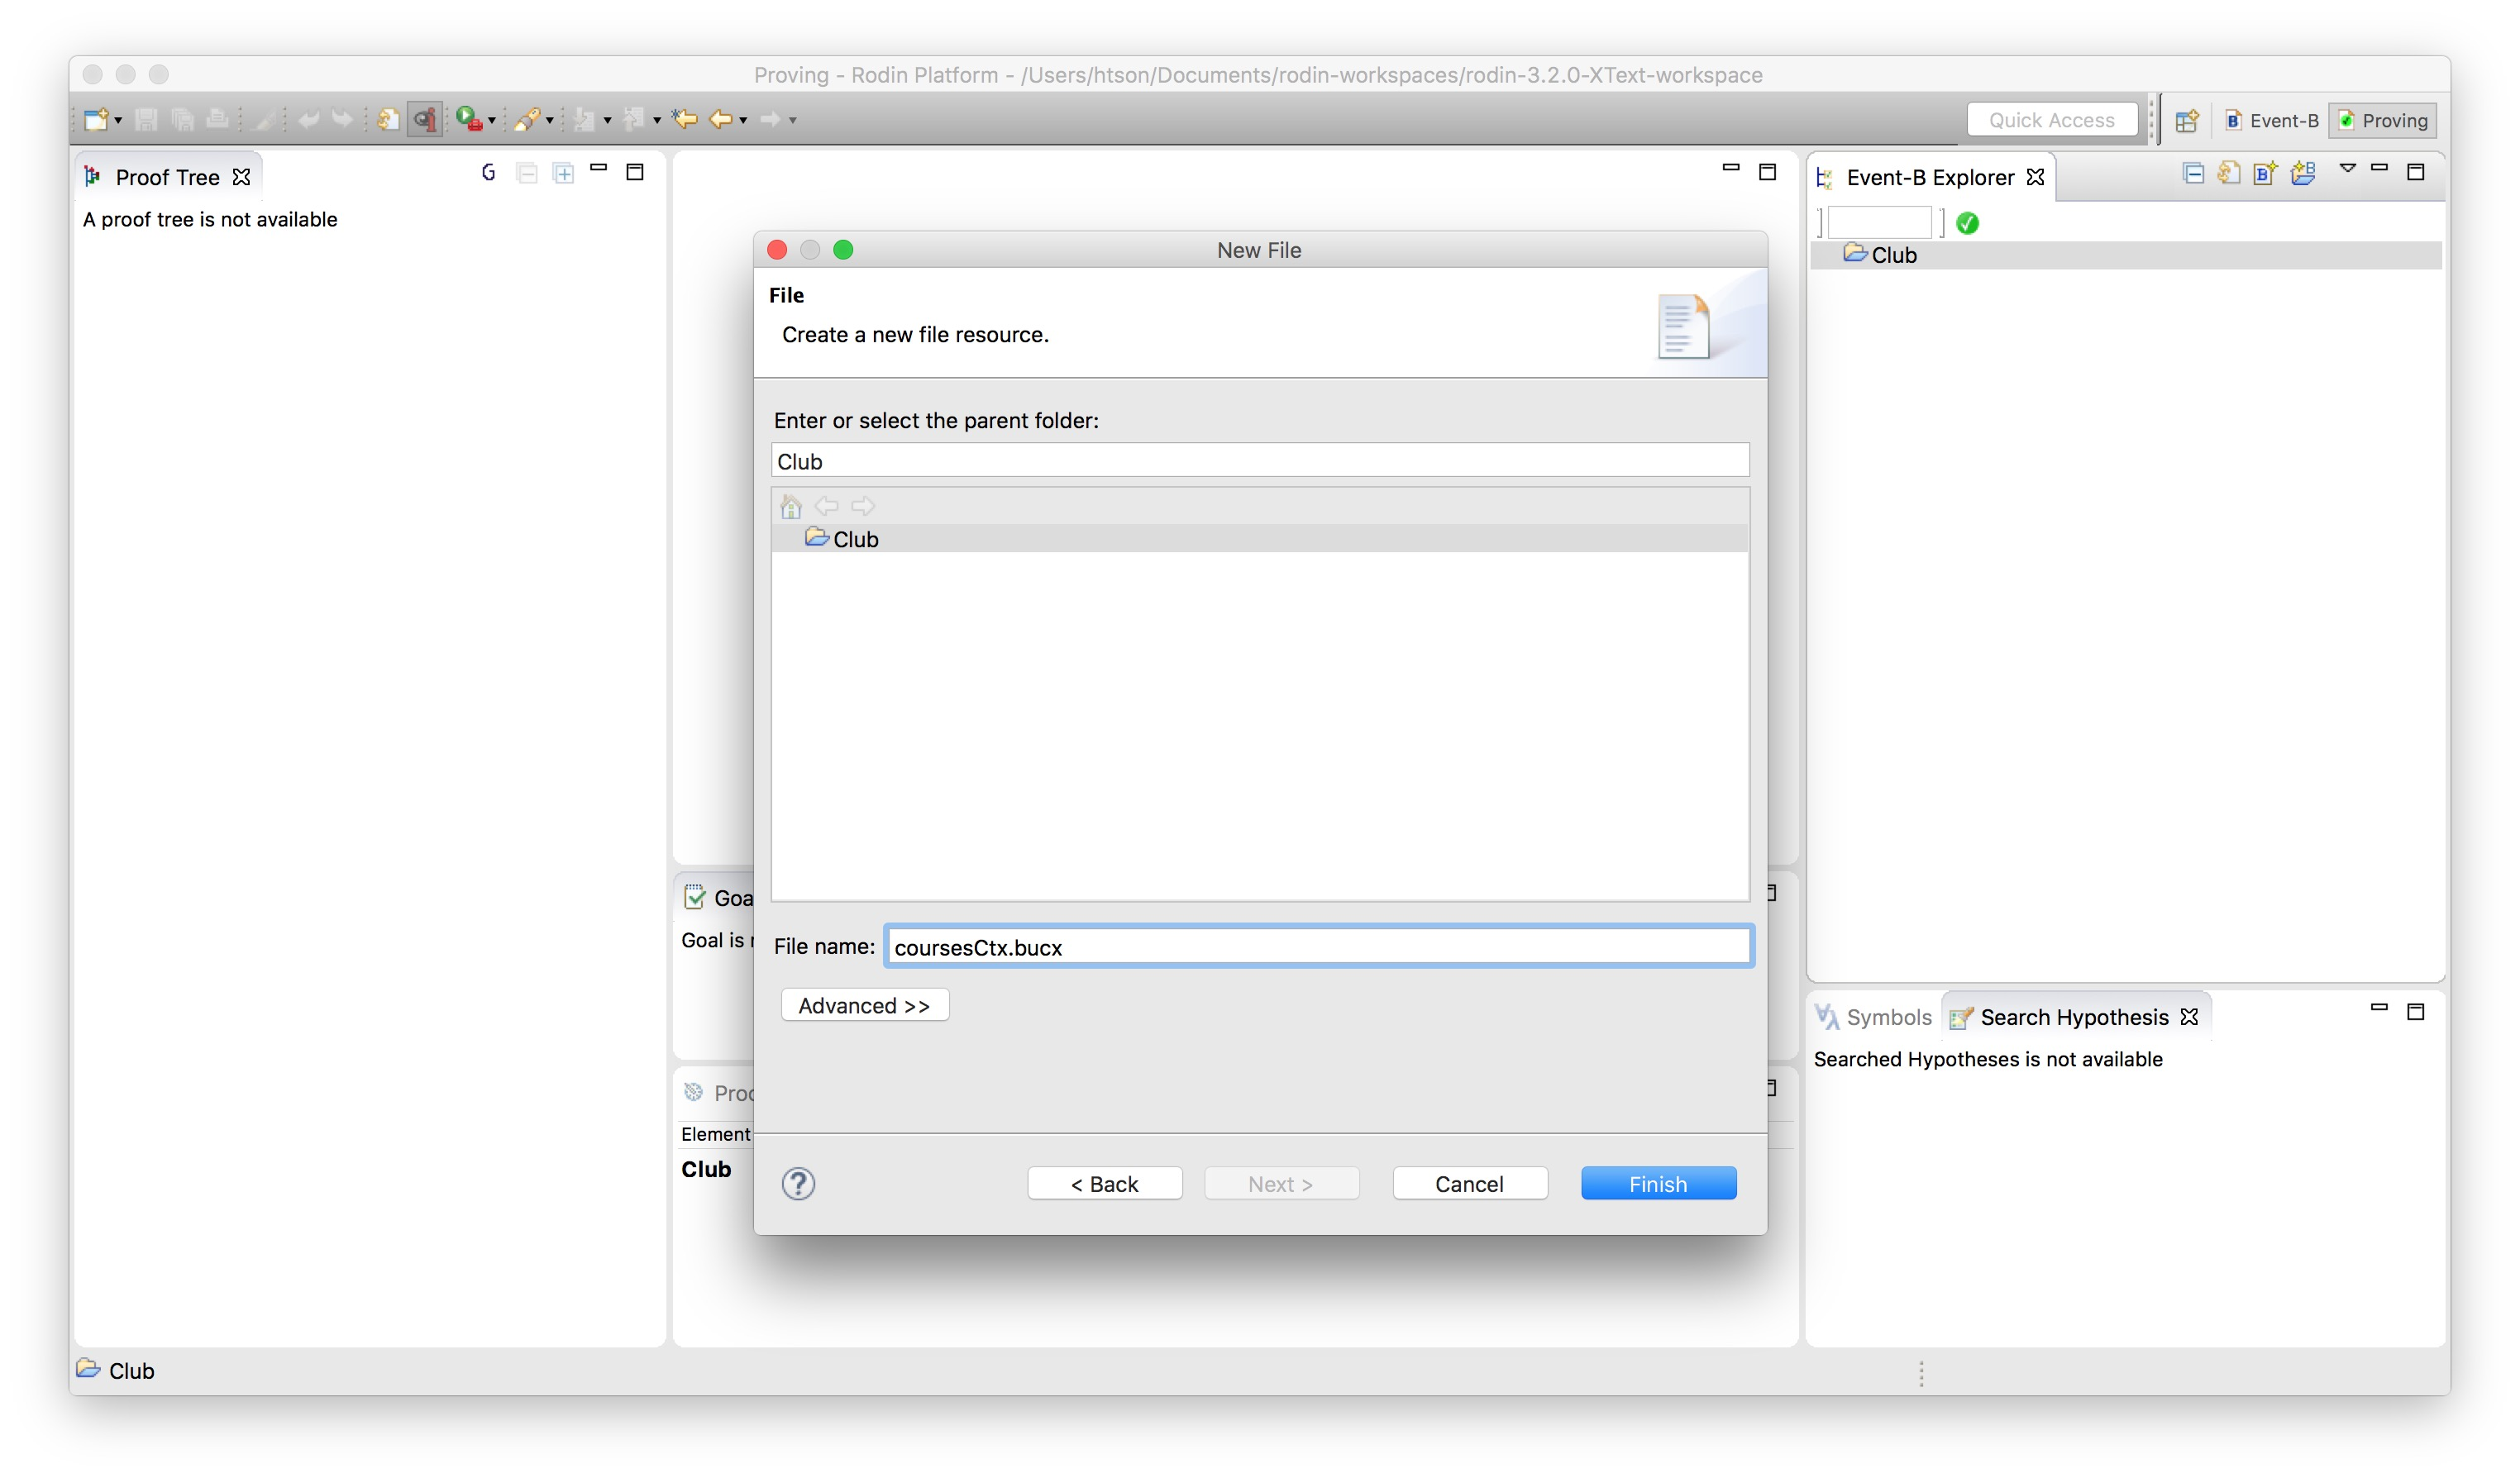
\includegraphics[width=512]{figures/CreateCoursesCtx}
  \else
  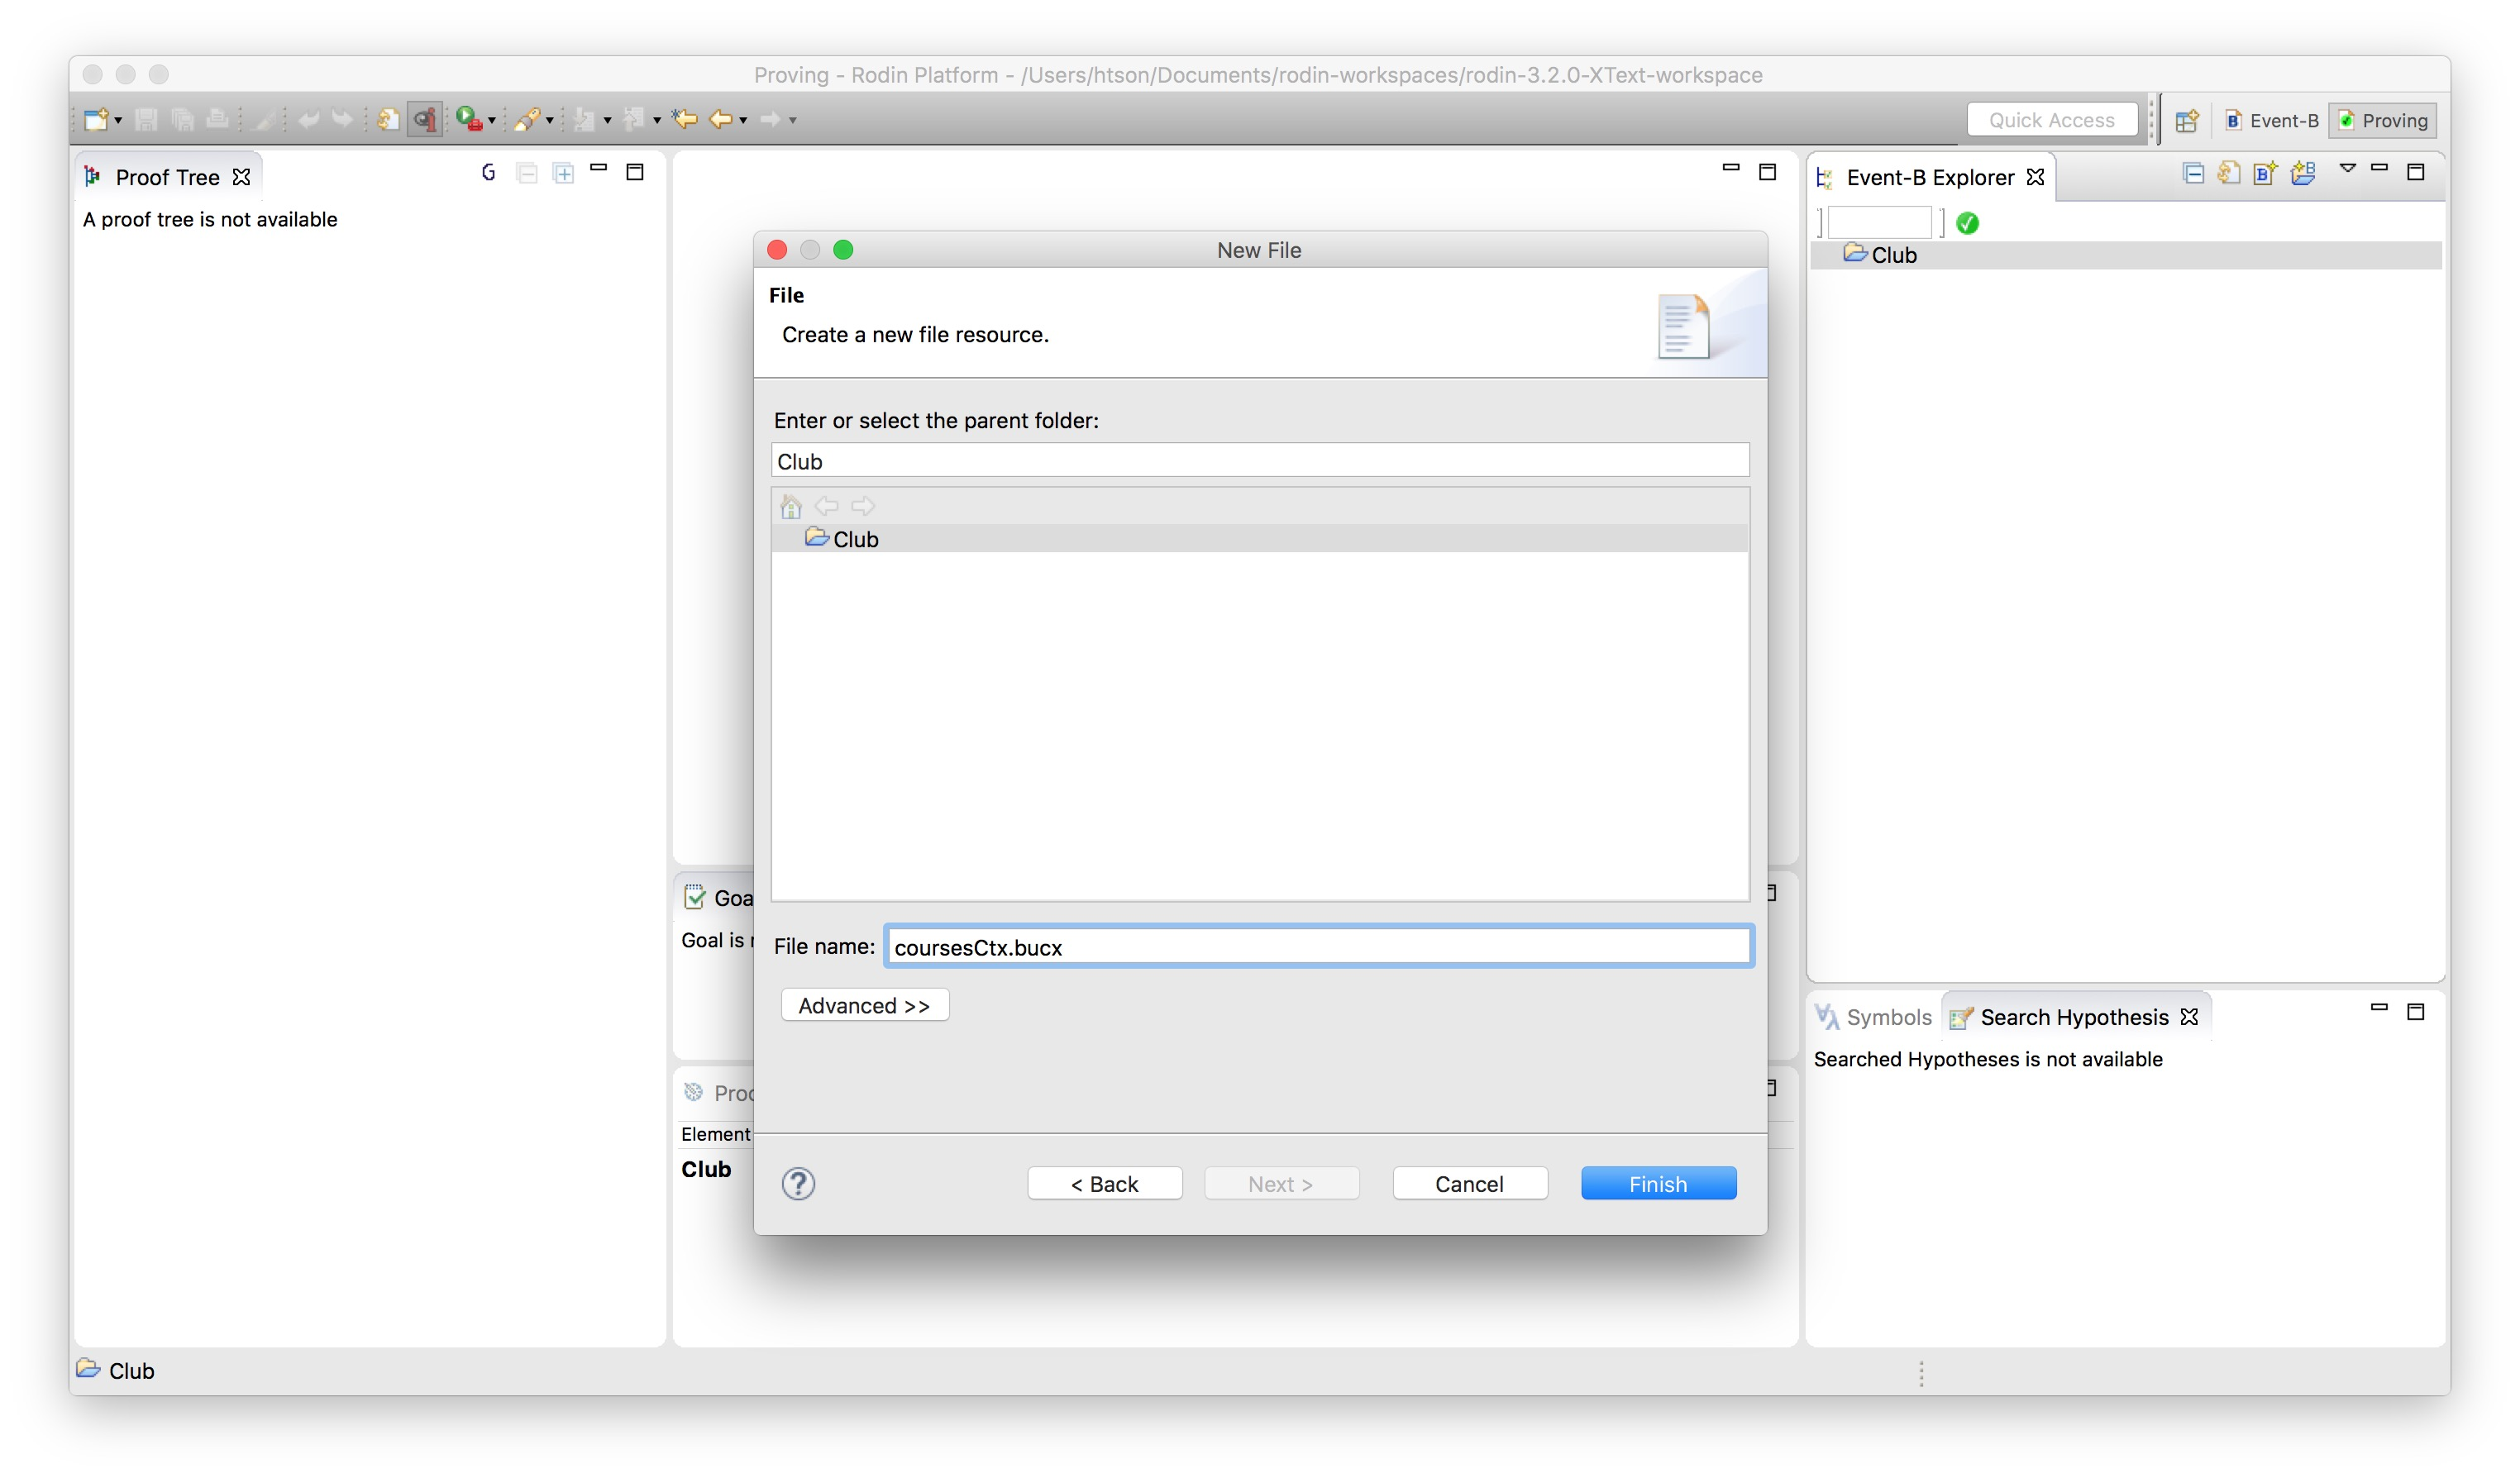
\includegraphics[width=0.9\textwidth]{figures/CreateCoursesCtx}
  \fi
  \caption{Create an XContext called ``coursesCtx.bucx''}
  \label{fig:CreateCoursesCtx}
\end{figure}
\begin{figure}[!htbp]
  \centering
  \ifplastex
  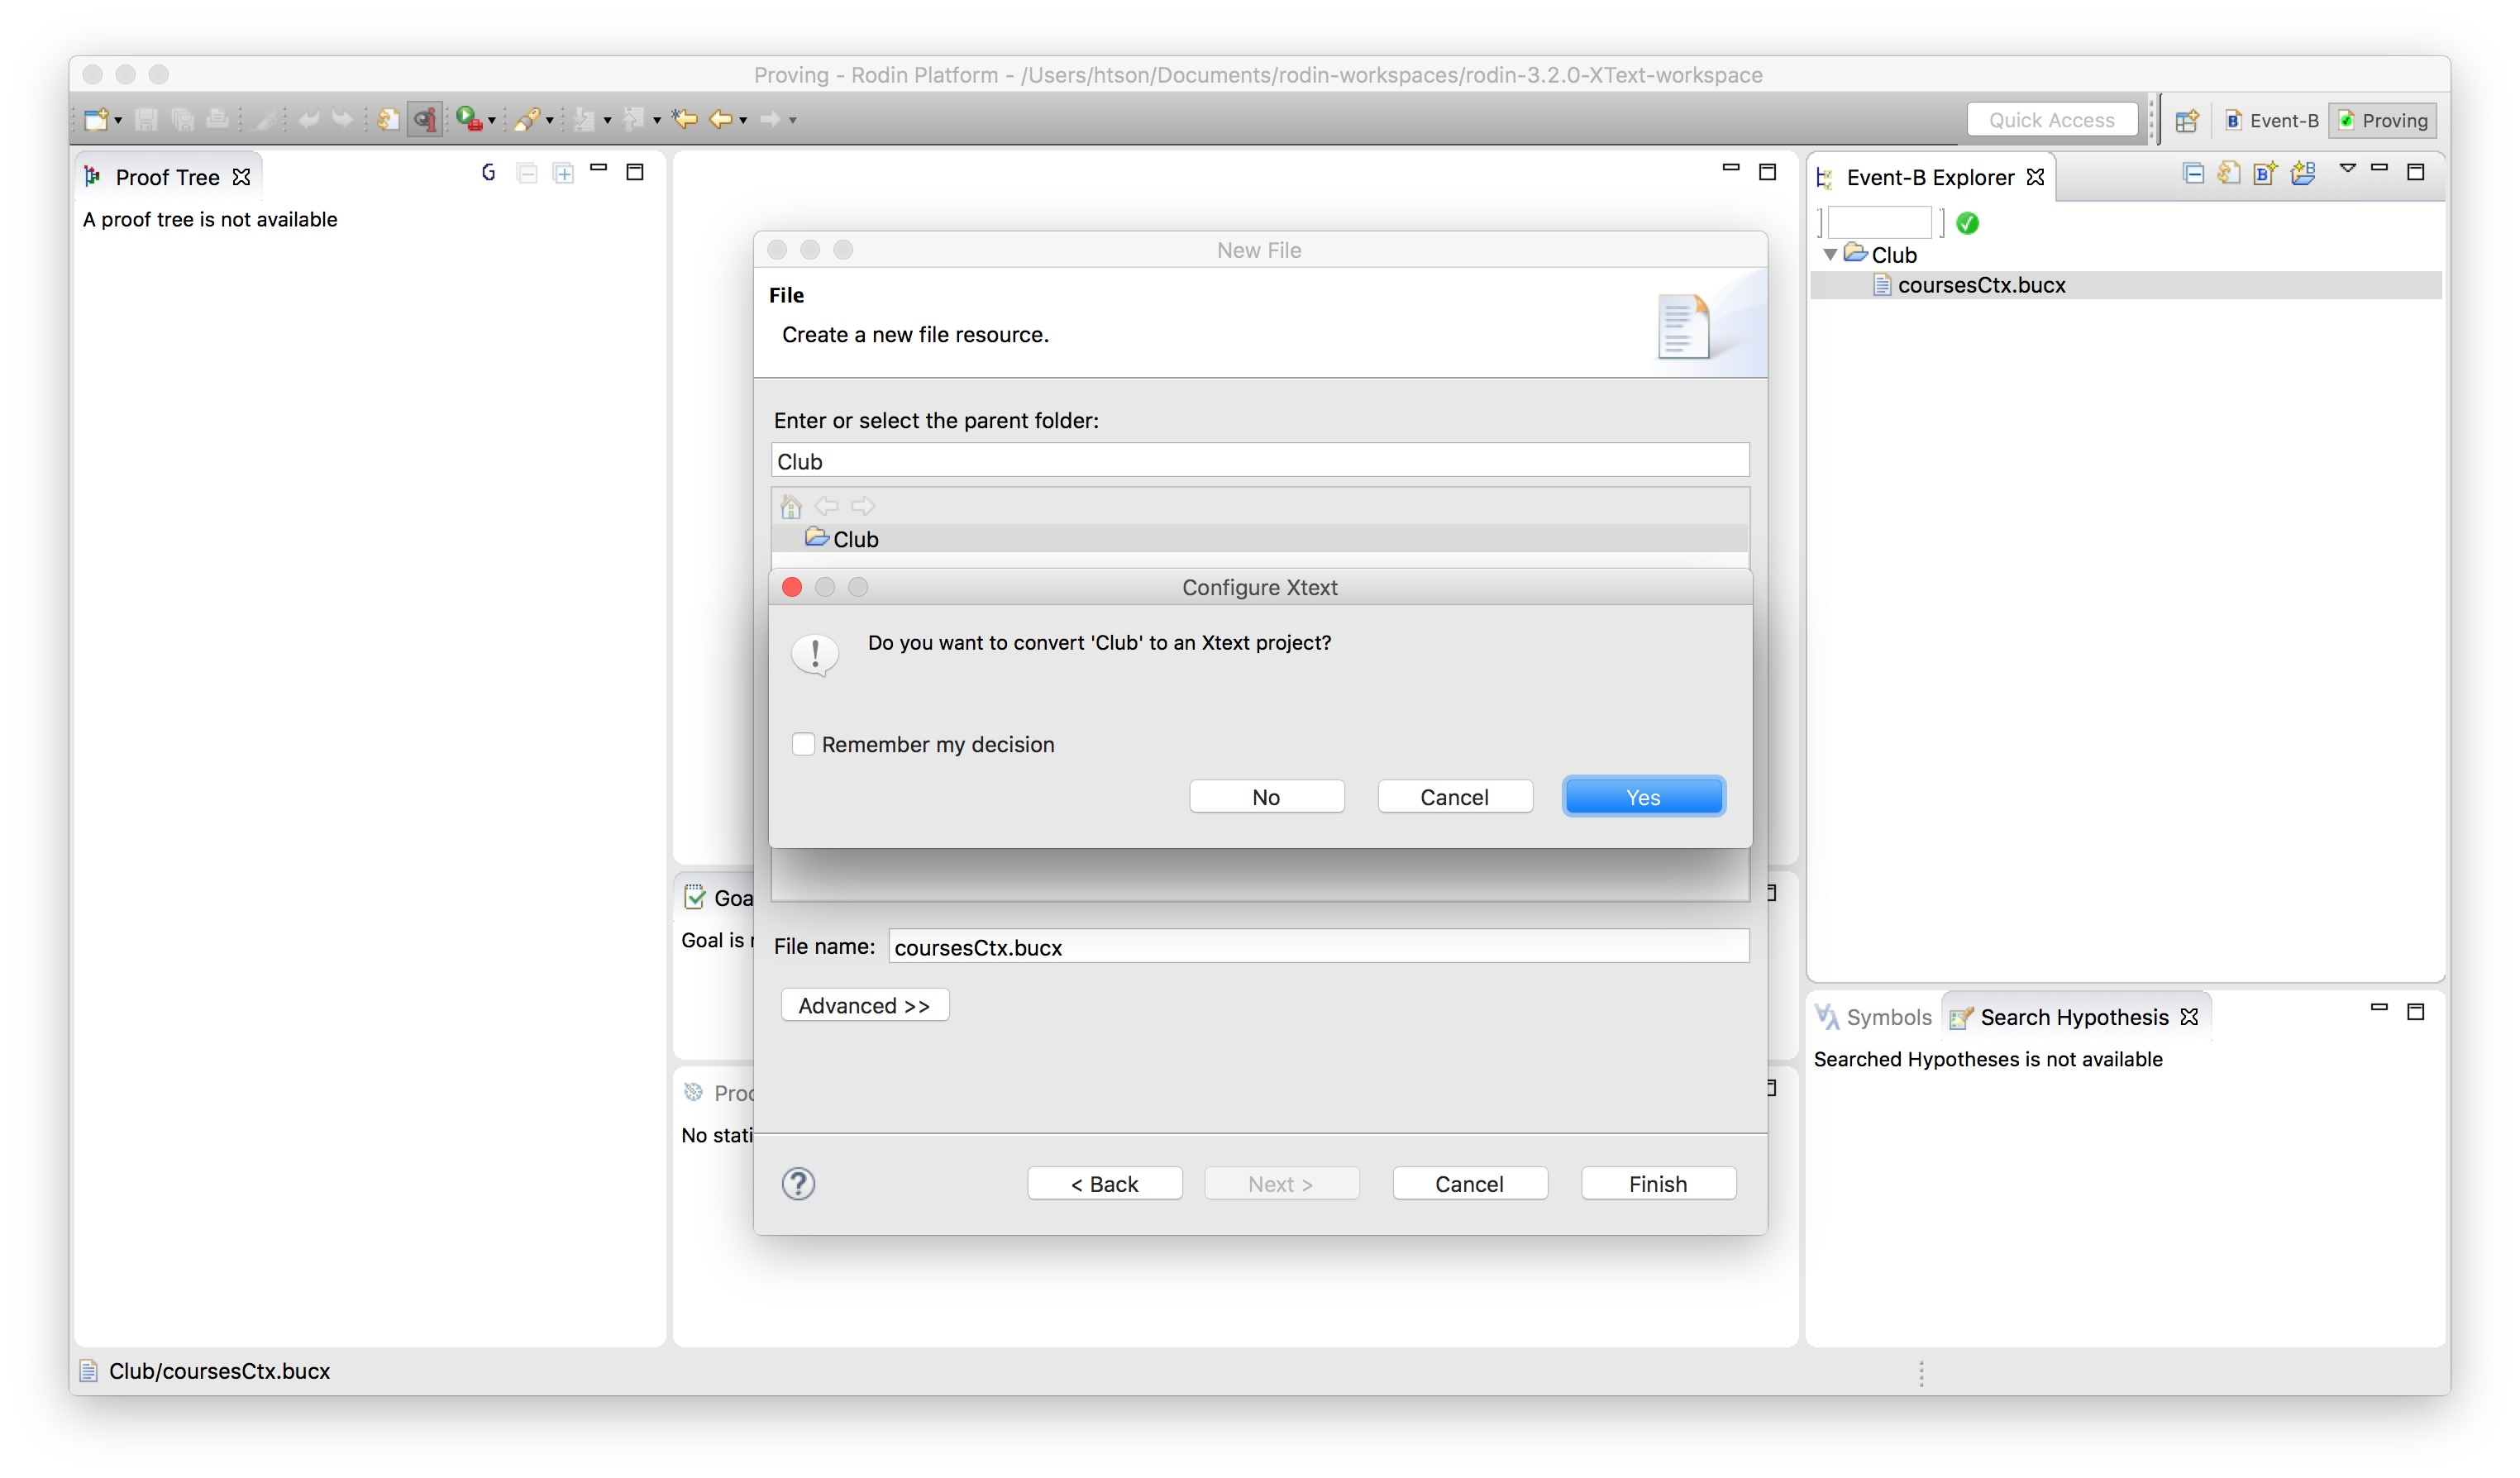
\includegraphics[width=512]{figures/ConvertToXText}
  \else
  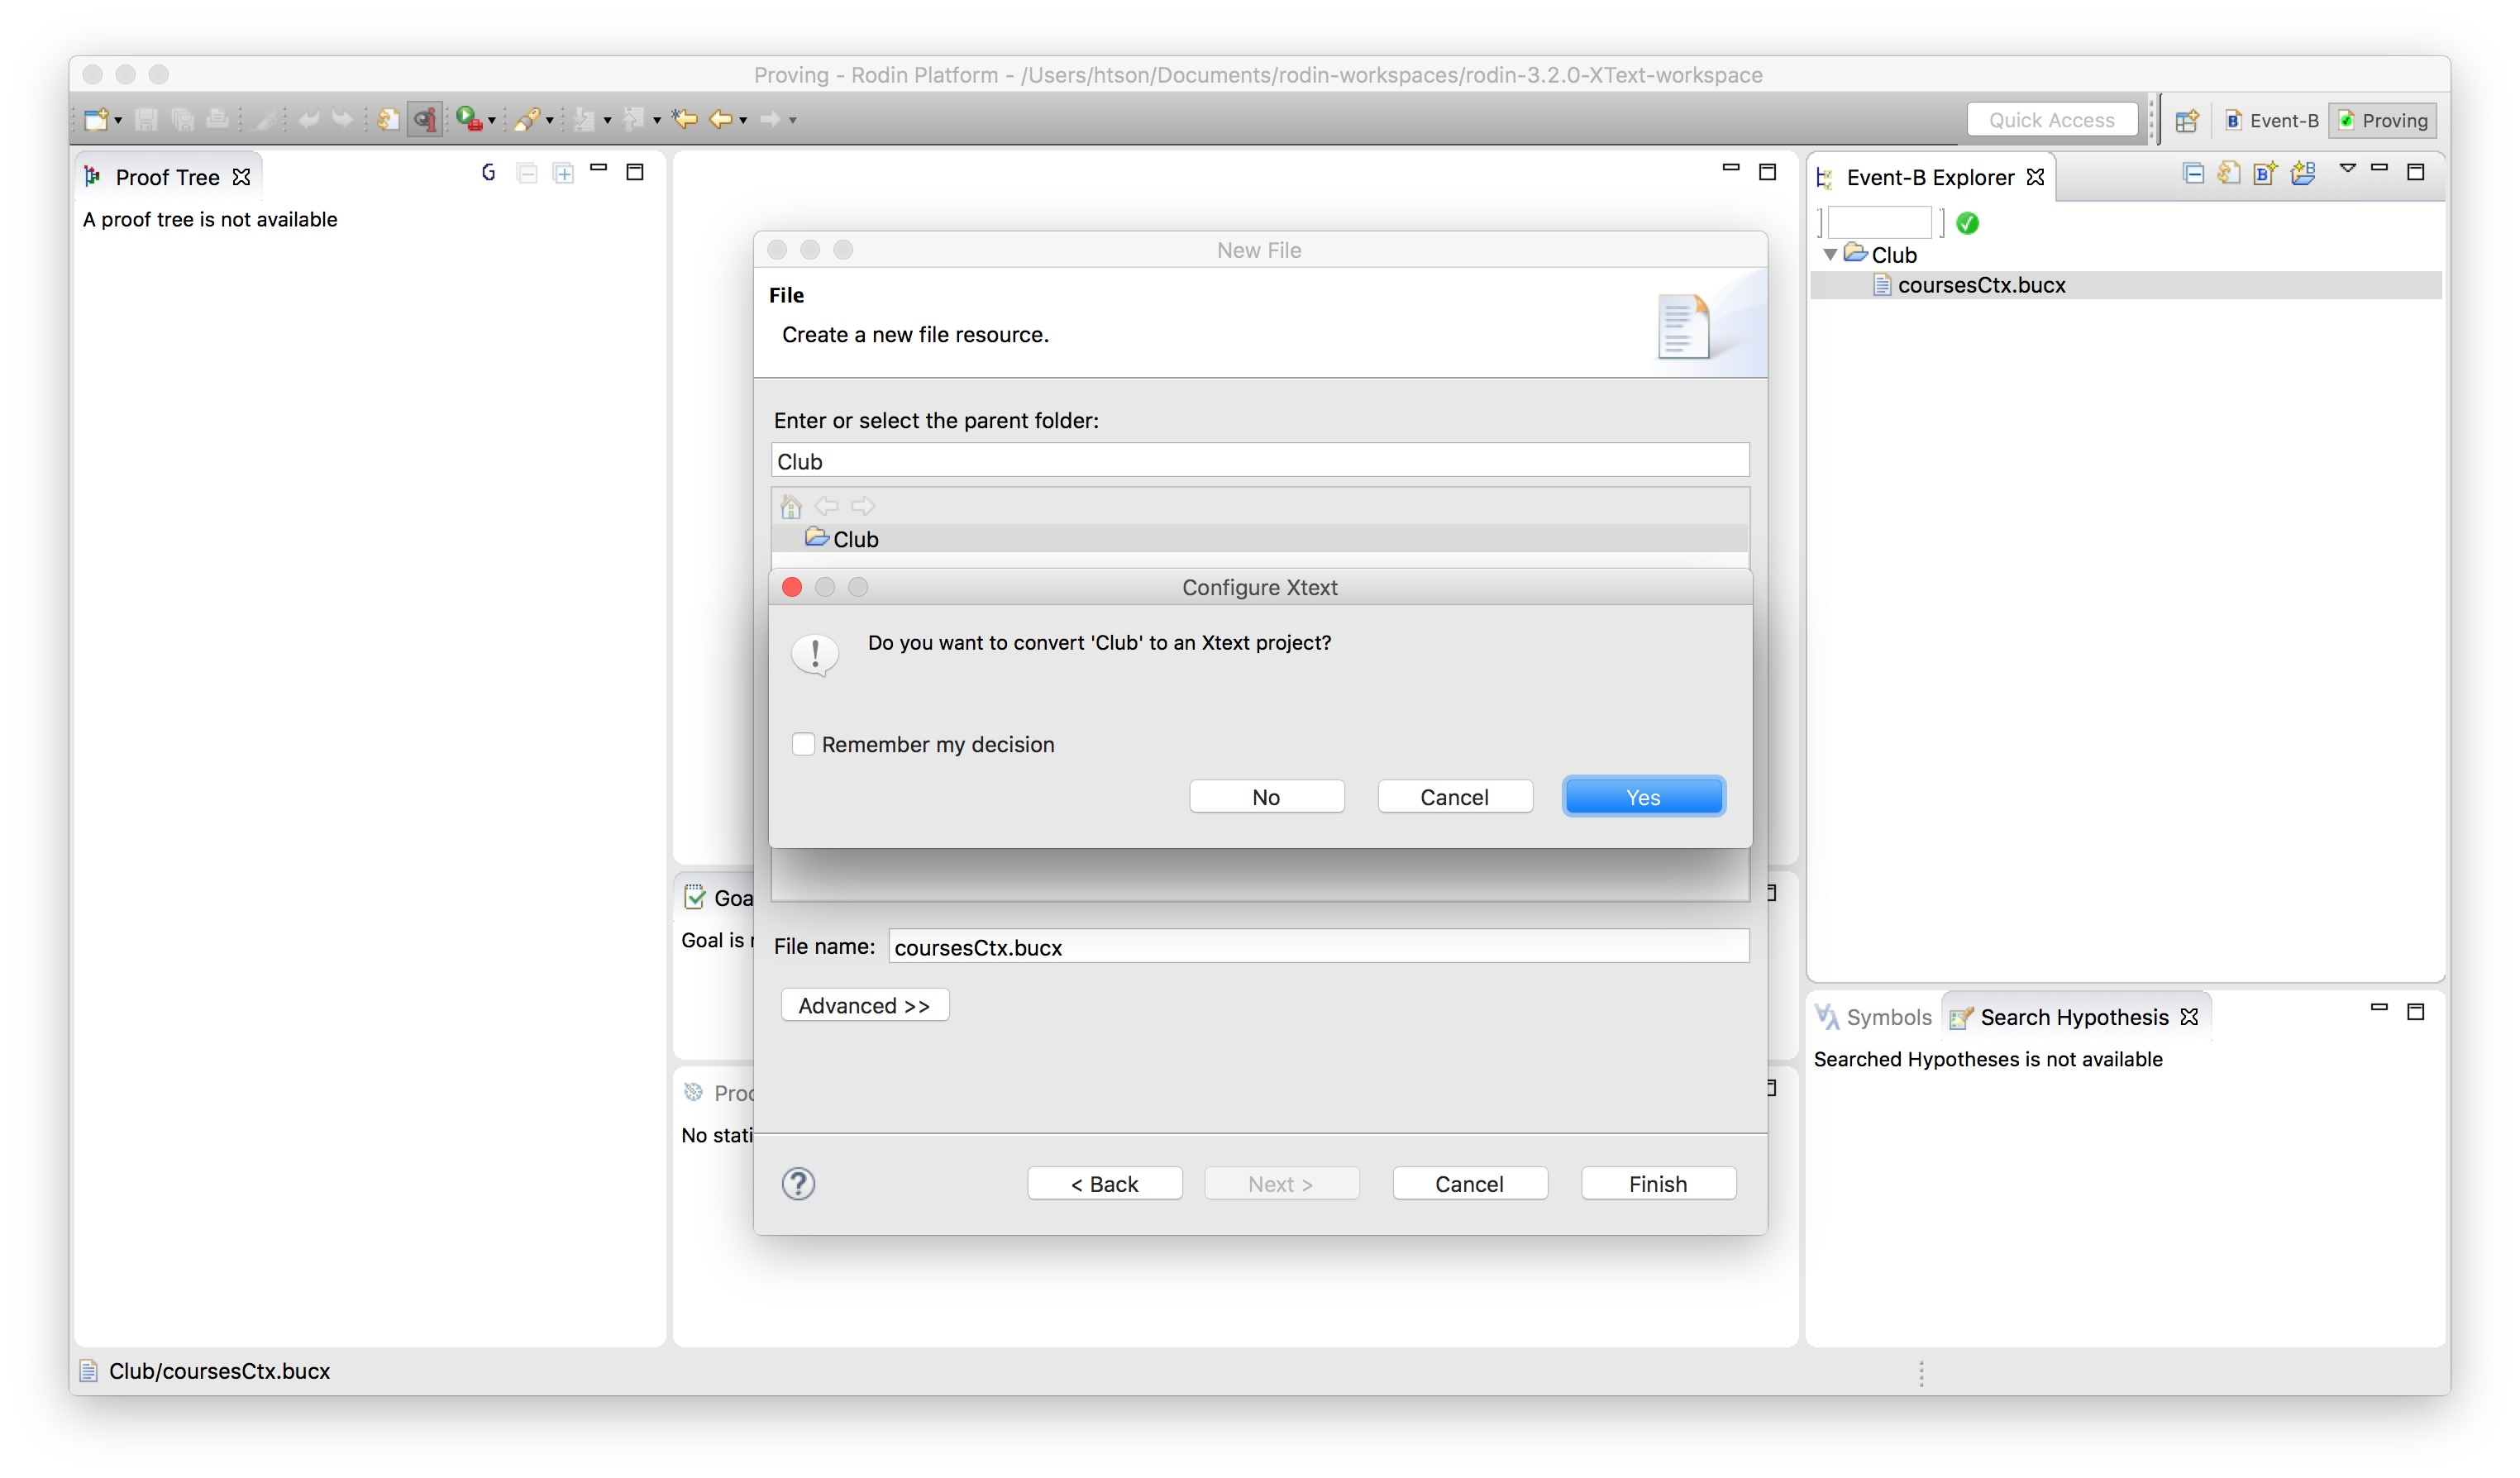
\includegraphics[width=0.9\textwidth]{figures/ConvertToXText}
  \fi
  \caption{Convert ``Club'' to XText project}
  \label{fig:ConvertToXText}
\end{figure}

\item[Step 2. Set the content of courseCtx.bucx] Set the content of ``coursesCtx.bucx'' as follows.
  \begin{center}
    \begin{Bcode}
      \ifplastex
      \Bcontext{} coursesCtx\\
      \Bsets{} CRS\\
      \Bconstants{} m\\
      \Baxioms\\
      @axm0_1: "finite(CRS)"\\
      @axm0_2: "m ∈ ℕ1"\\
      @thm0_1: "0 < m" \Btheorem\\
      \Bend
      \else
\Bcontext{} coursesCtx\\
\Bsets{} CRS\\
\Bconstants{} m\\
\Baxioms\\
\Btab @axm0\_1: "\(\finite(CRS)\)"\\
\Btab @axm0\_2: "\(m \in \natn\)"\\
\Btab @thm0\_1: "\(0 < m\)" \Btheorem\\
\Bend
       \fi
    \end{Bcode}
  \end{center}
  \textbf{Important}: In order to typeset Event-B mathematical symbol, e.g., \ifplastex ℕ1 \else $\natn$ \fi, one can use content assist. For example, typing \texttt{NAT} and invoking content assist (e.g., on Mac OS \texttt{Ctrl+Space}), a dropdown list will appear with options for typesetting \ifplastex ℕ \else $\natn$ \fi and \ifplastex ℕ1 \else $\natn$ \fi (See Figure~\ref{fig:NAT1ContentAssist}.
  \begin{figure}[!htbp]
    \centering
    \ifplastex
    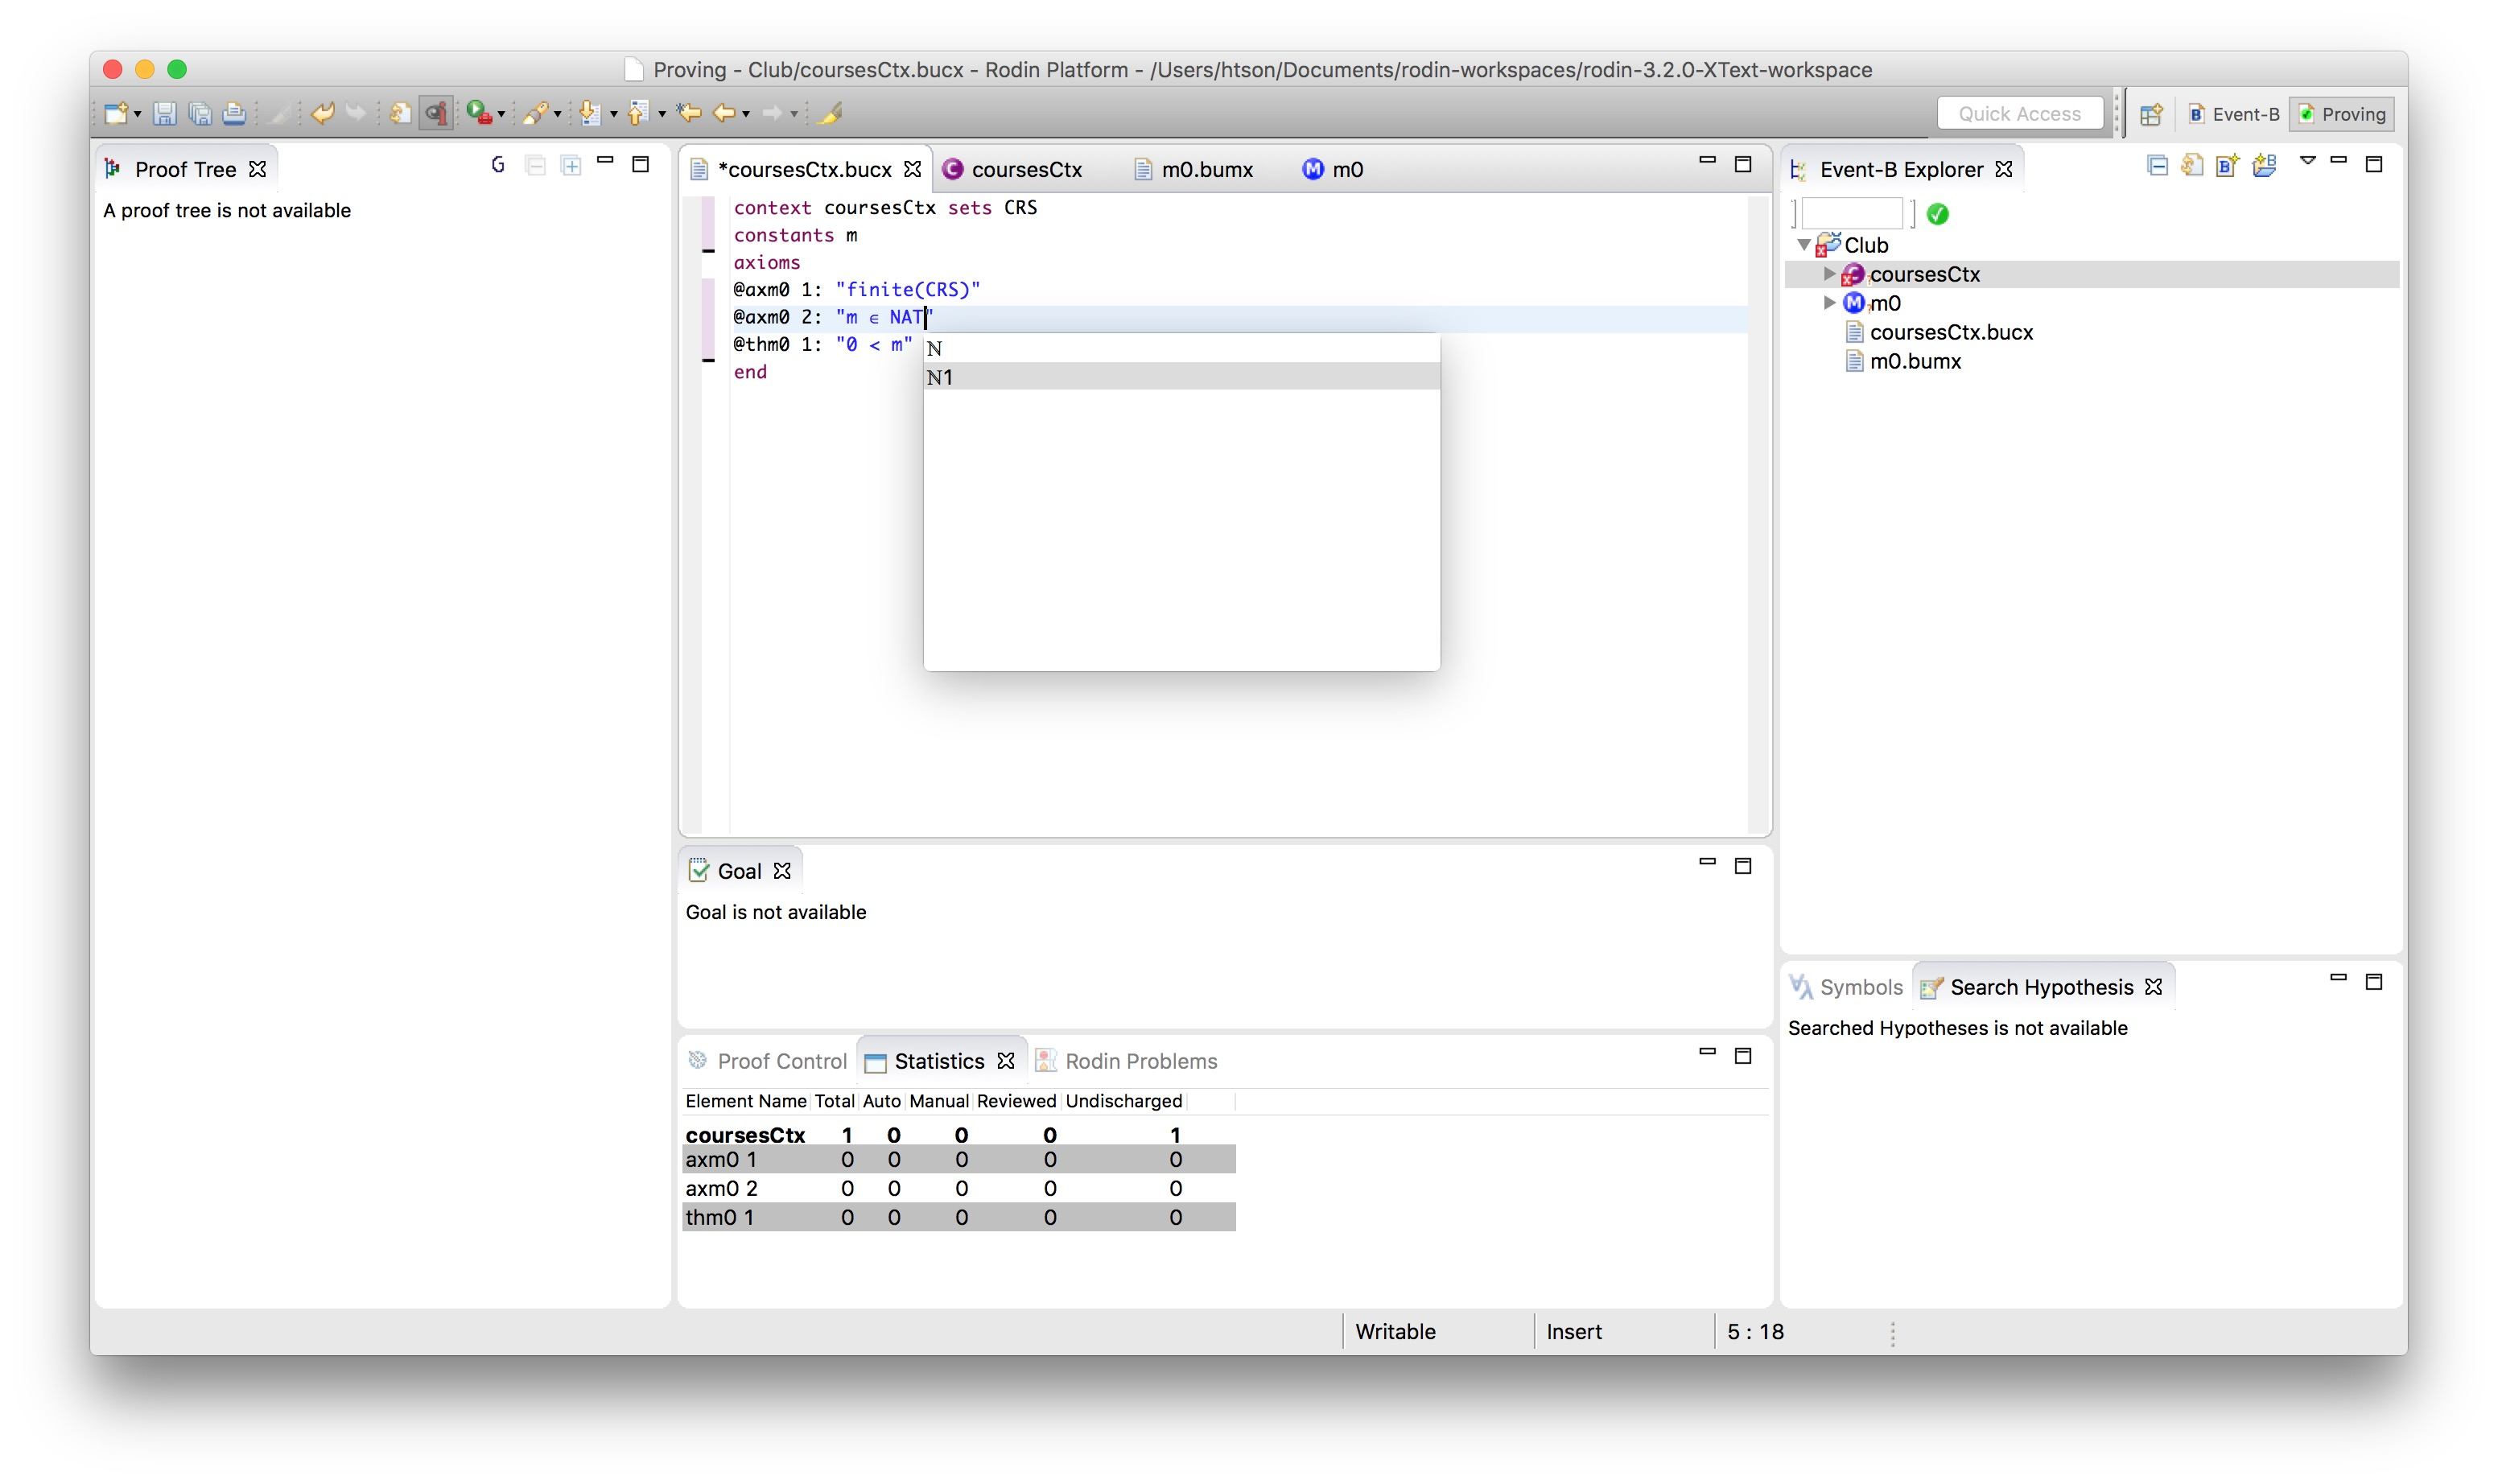
\includegraphics[width=512]{figures/NAT1ContentAssist}
    \else
    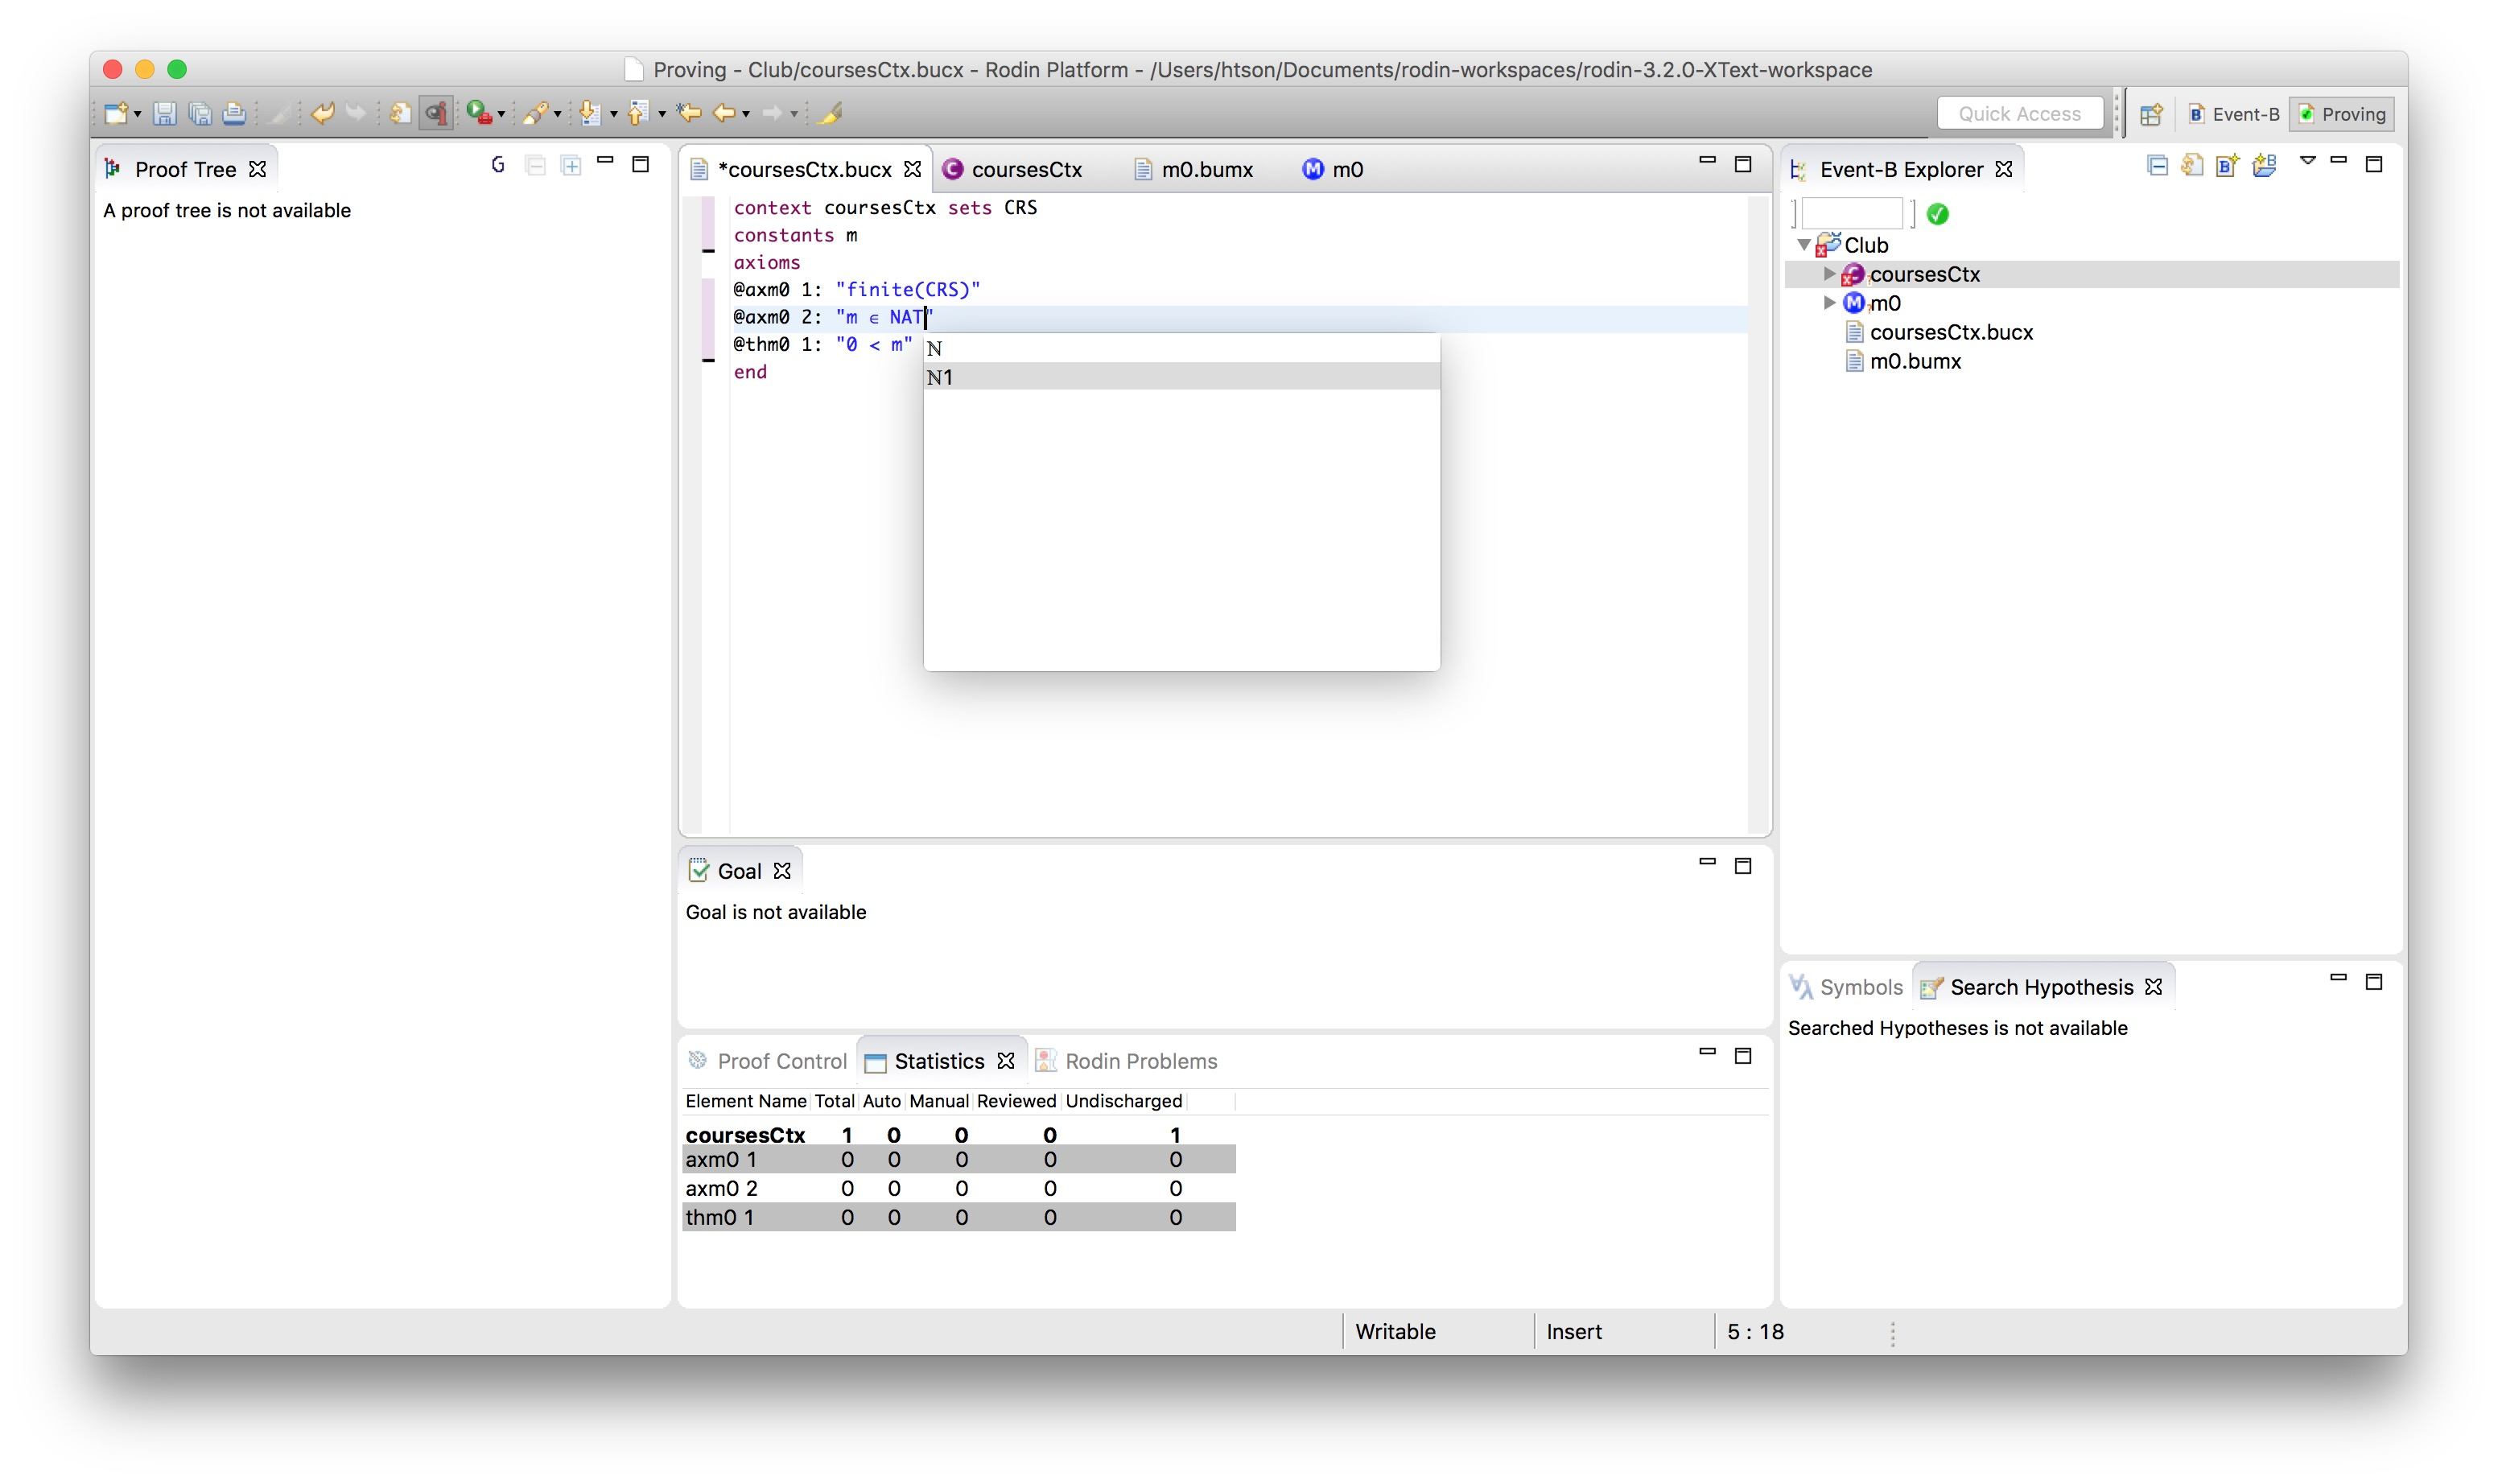
\includegraphics[width=0.9\textwidth]{figures/NAT1ContentAssist}
    \fi
    \caption{Type-setting \ifplastex ℕ1 \else $\natn$ \fi using Content Assist}
    \label{fig:NAT1ContentAssist}
  \end{figure}

\item[Step 3. Auto-format the code] Automatically format the content of ``coursesCtx.bucx'' using short-cut (e.g., on Mac OS: \texttt{Cmd+Shift+F}).

\item[Step 4. Save the file] \textbf{Save the file ``coursesCtx.bucx''}.
\end{description}
\textbf{Conclusion} By now, the XContext ``coursesCtx.bucx'' and the corresponding Rodin Context ``coursesCtx'' should be visible in the Event-B Explorer (see Figure~\ref{fig:CoursesCtx}). 
  \begin{figure}[!htbp]
    \centering
    \ifplastex
    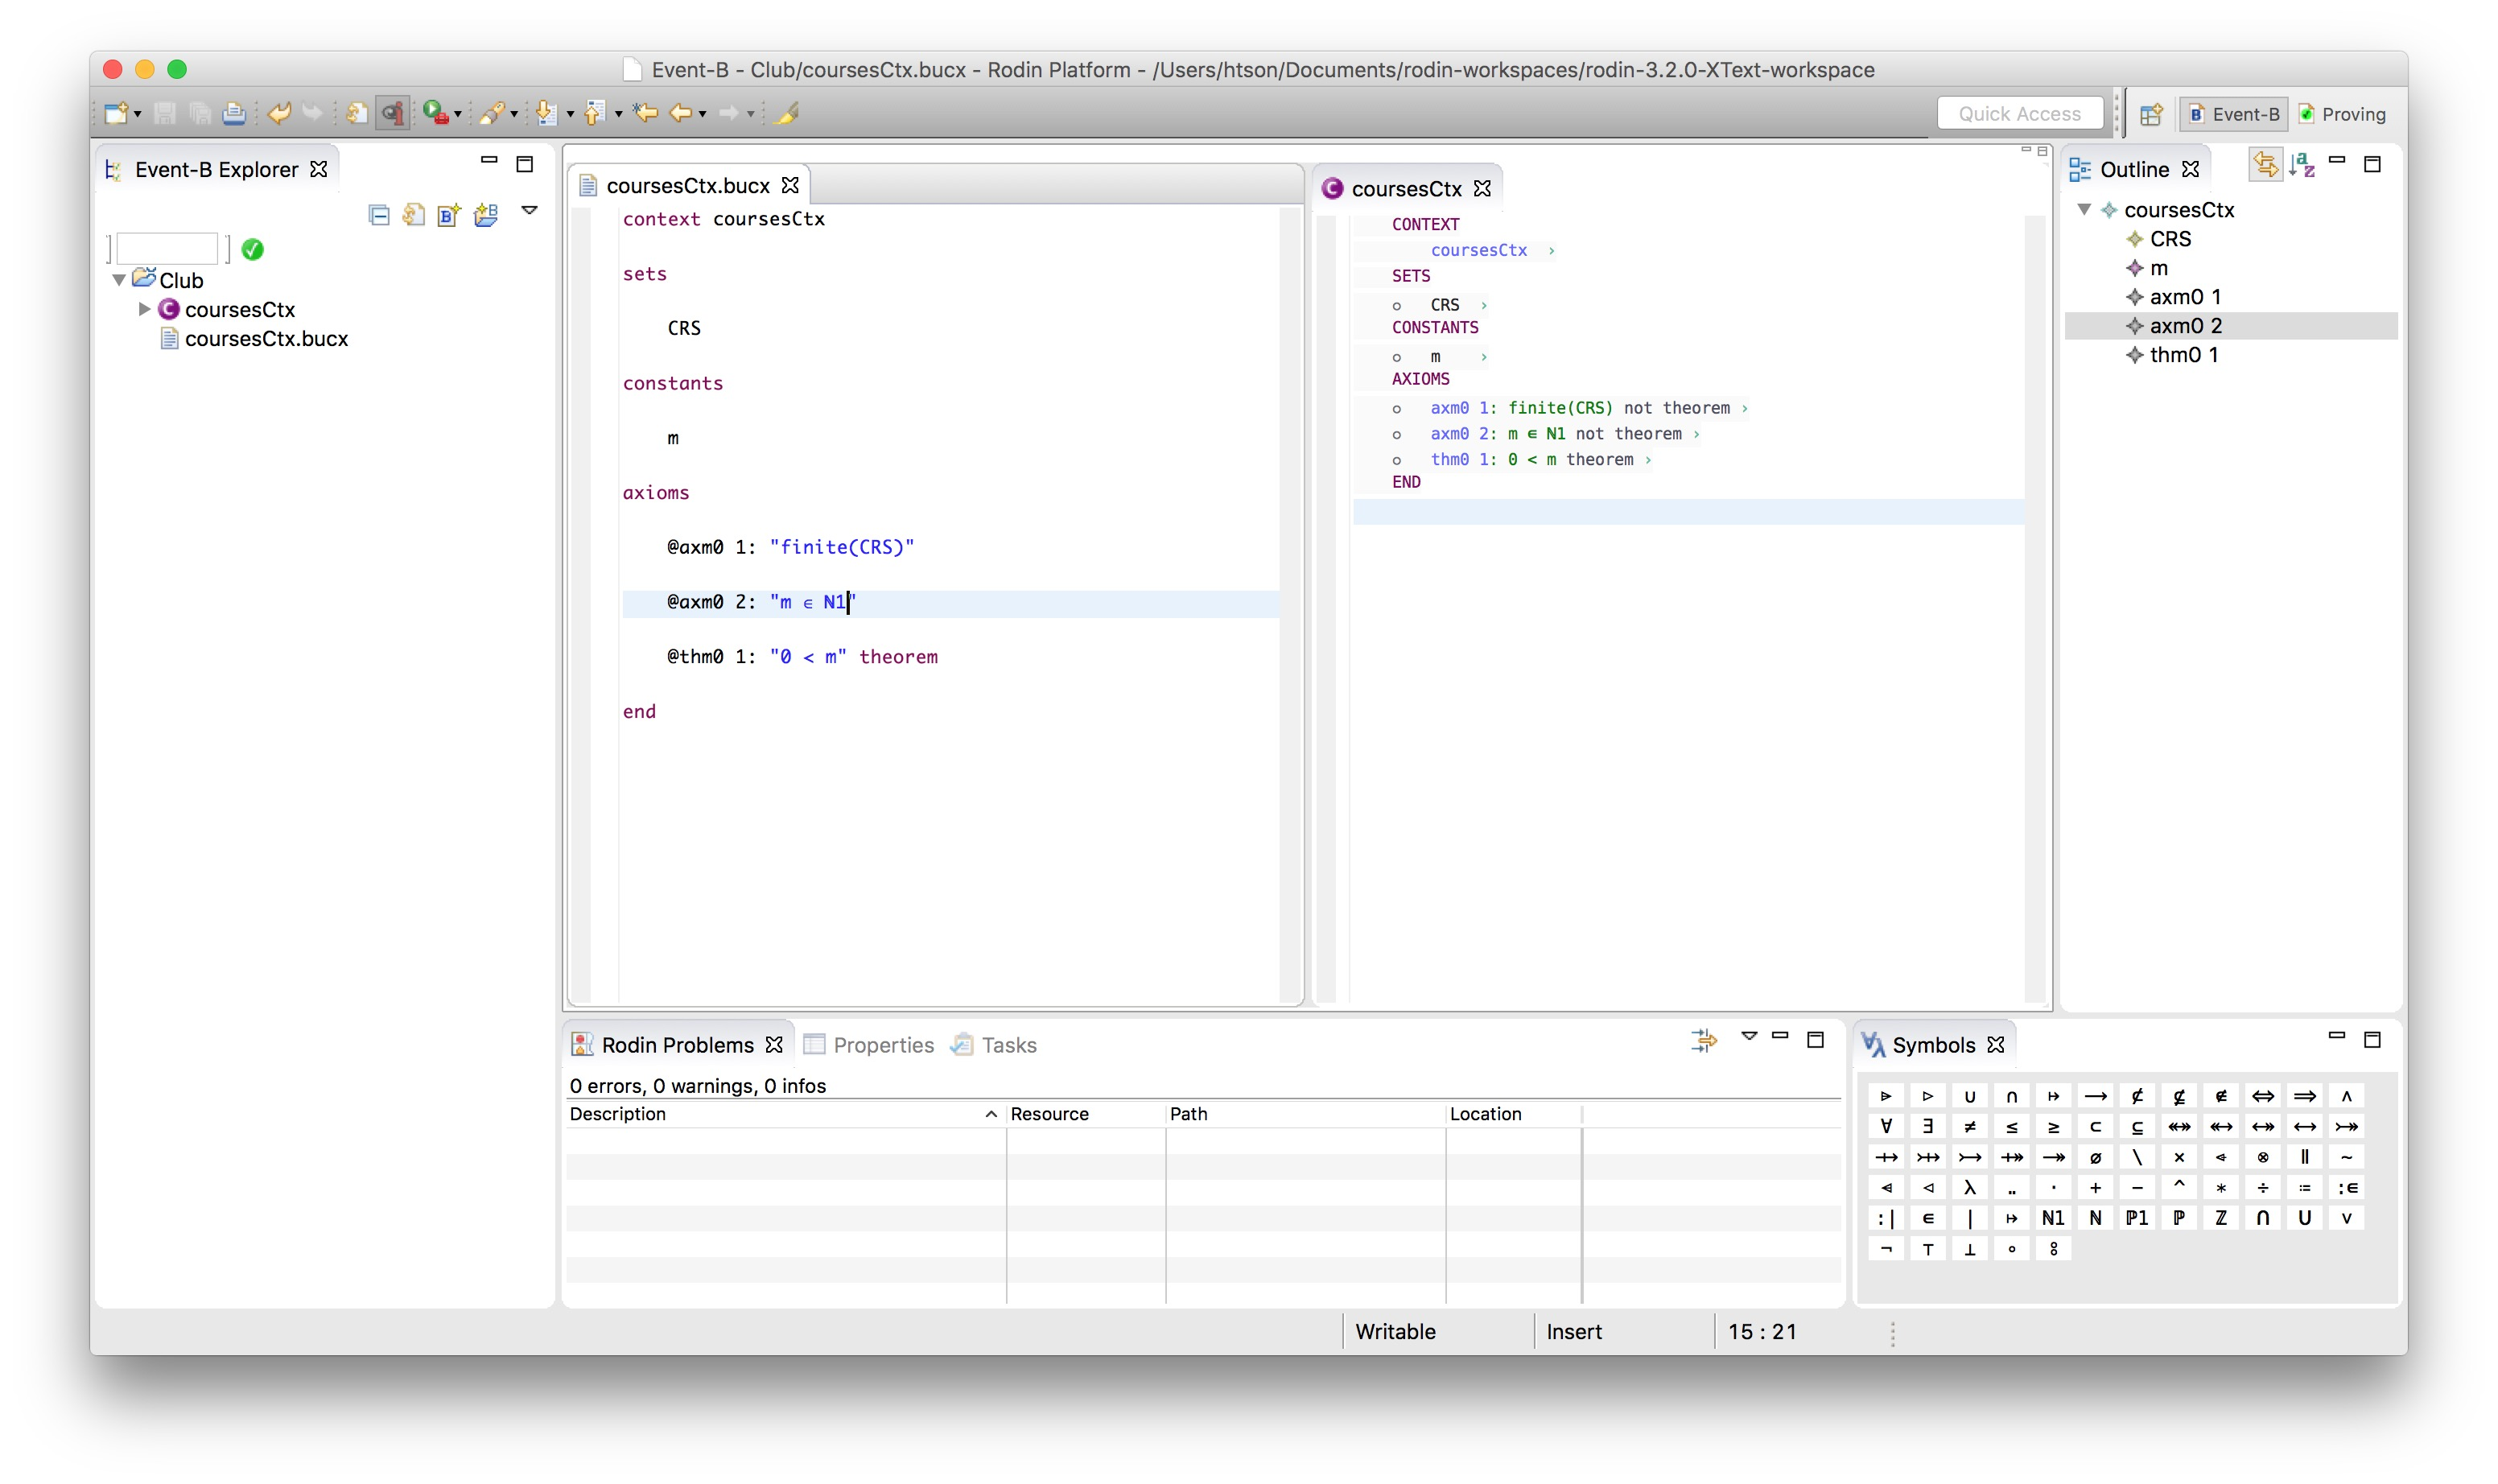
\includegraphics[width=512]{figures/CoursesCtx}
    \else
    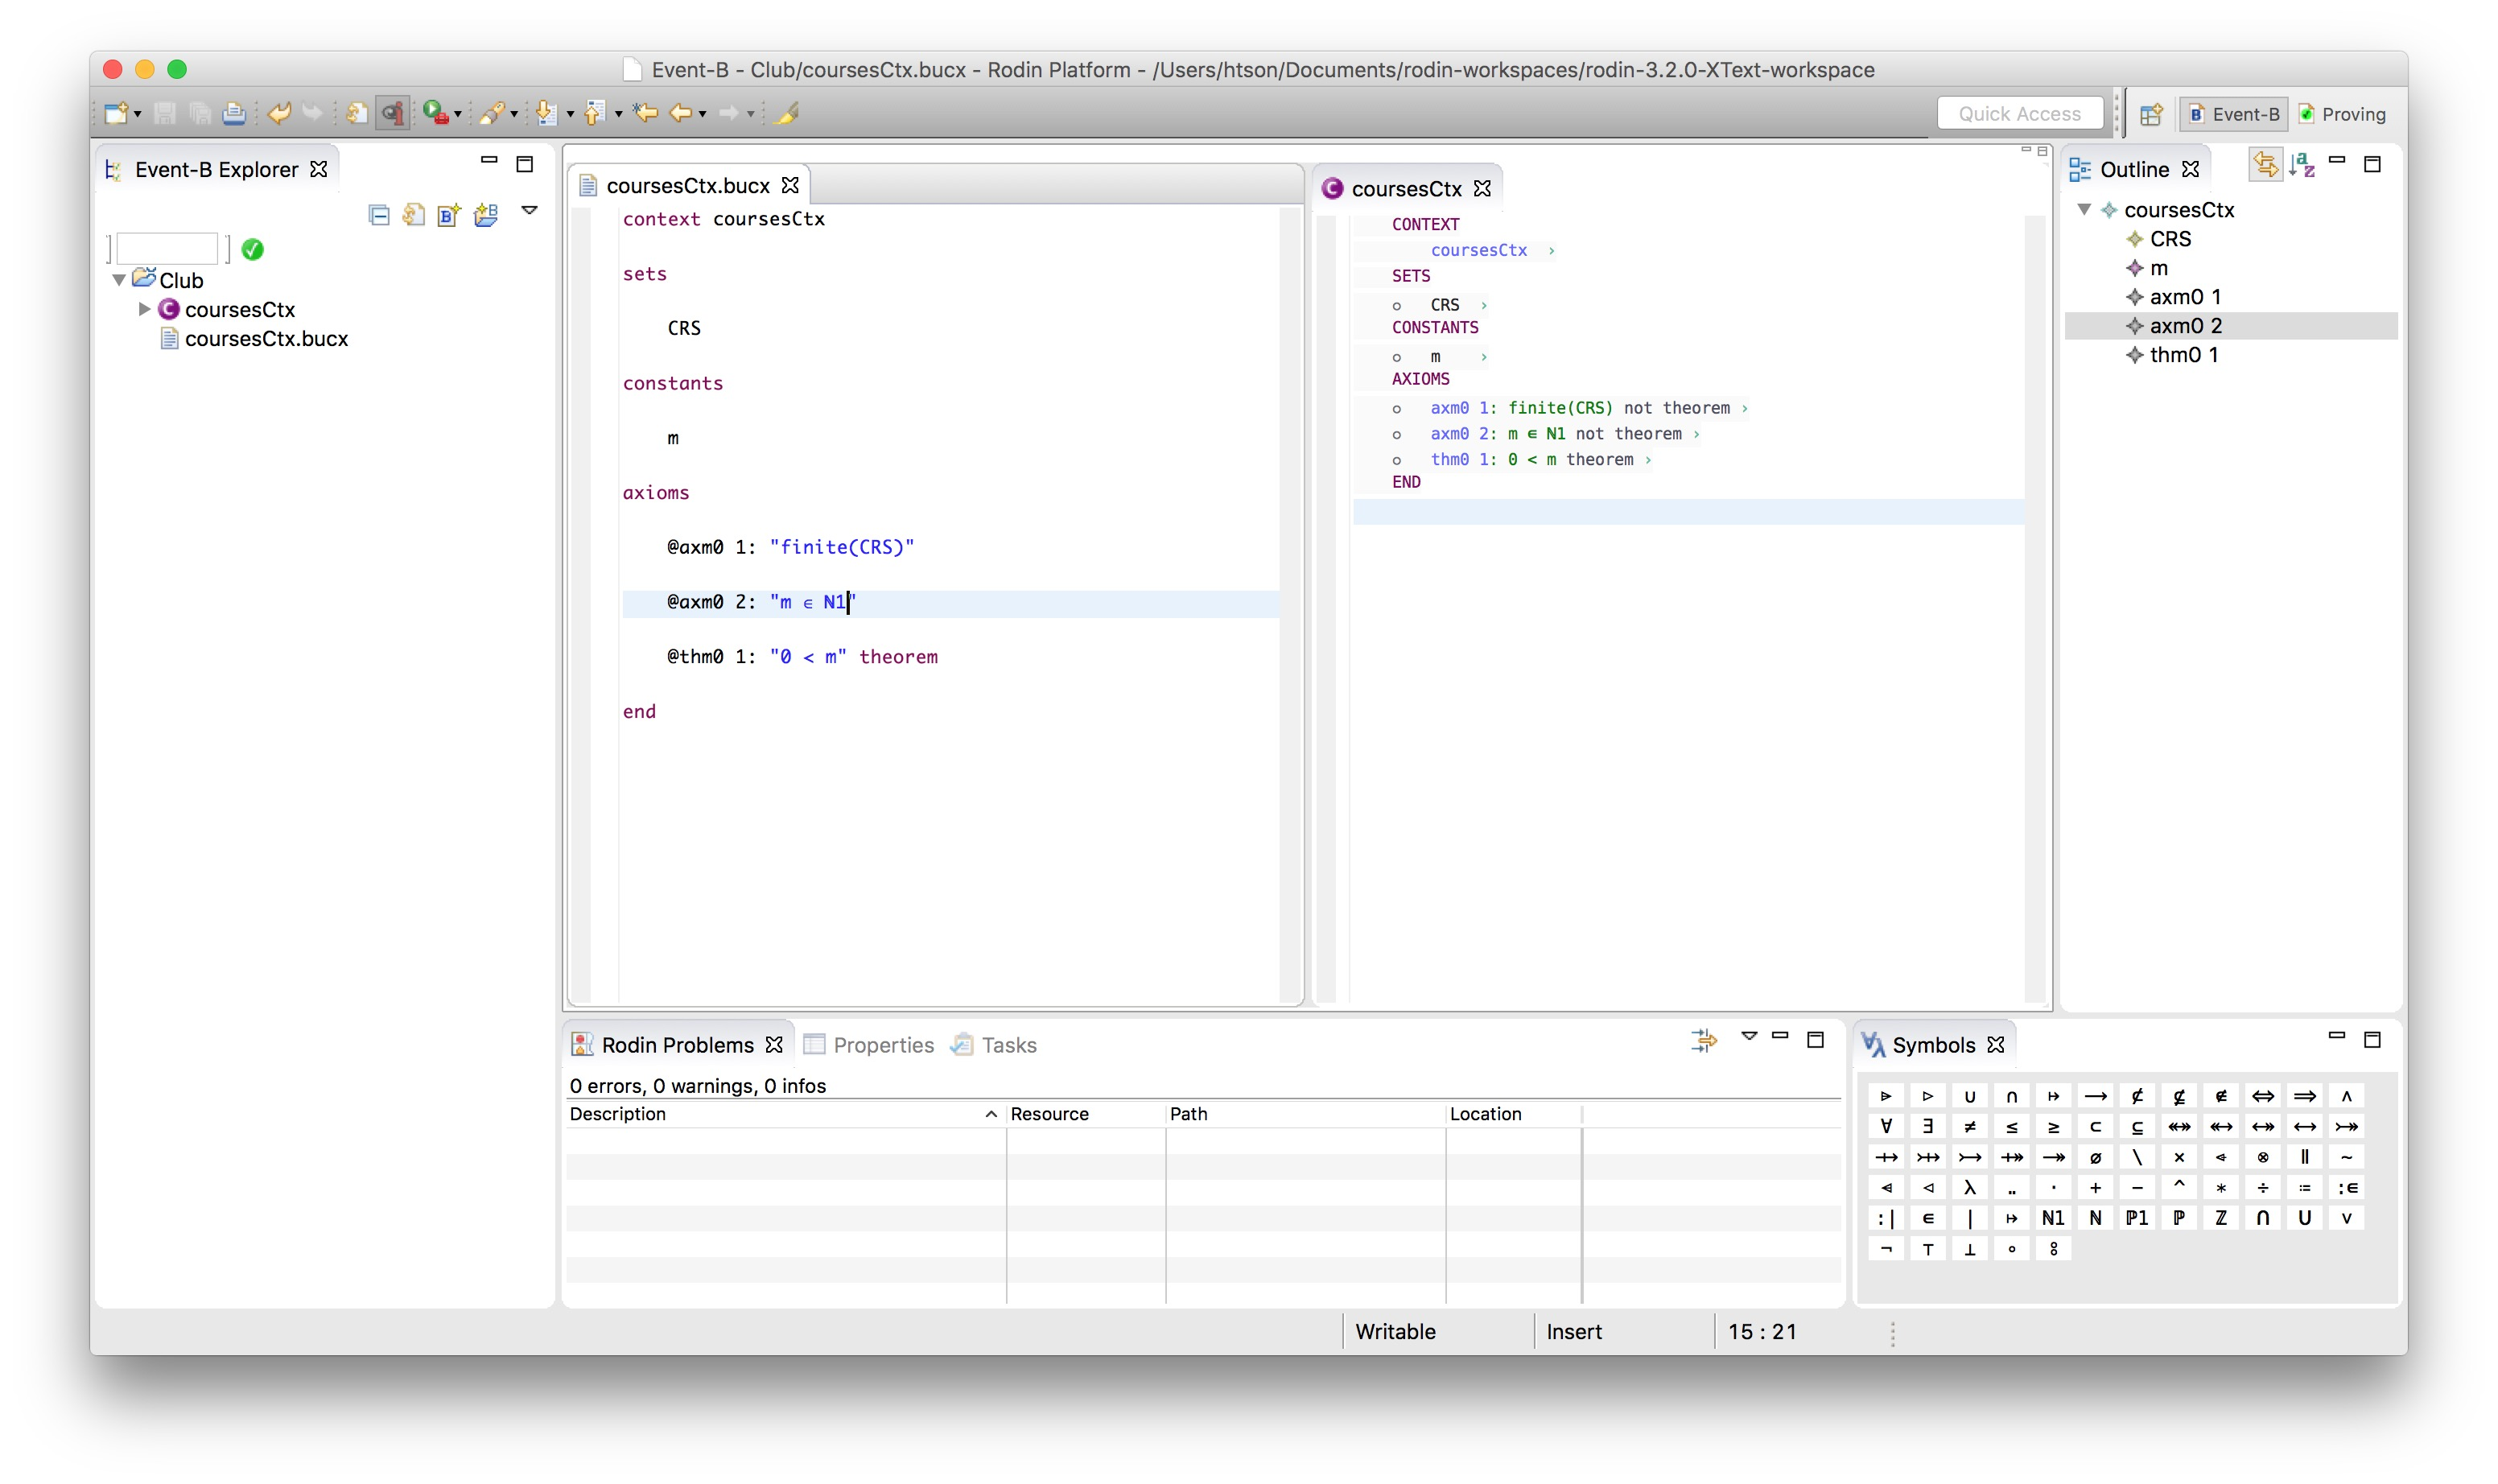
\includegraphics[width=0.9\textwidth]{figures/CoursesCtx}
    \fi
    \caption{The final XContext coursesCtx.bucx}
    \label{fig:CoursesCtx}
  \end{figure}



\subsubsection{Task 4. Create a simple XMachine m0.bumx}\label{CreateMachine}
\textbf{Introduction} The purpose of this task is to create a simple XMachine within the newly created project.

\begin{description}
\item[Step 1. Create a new XMachine m0.bumx] \textbf{Create a new XMachine} named ``m0.bumx'' using the New File wizard (see Figure~\ref{fig:CreateM0}. The newly created file should be opened automatically in an XMachine editor.
  \begin{figure}[!htbp]
    \centering
    \ifplastex
    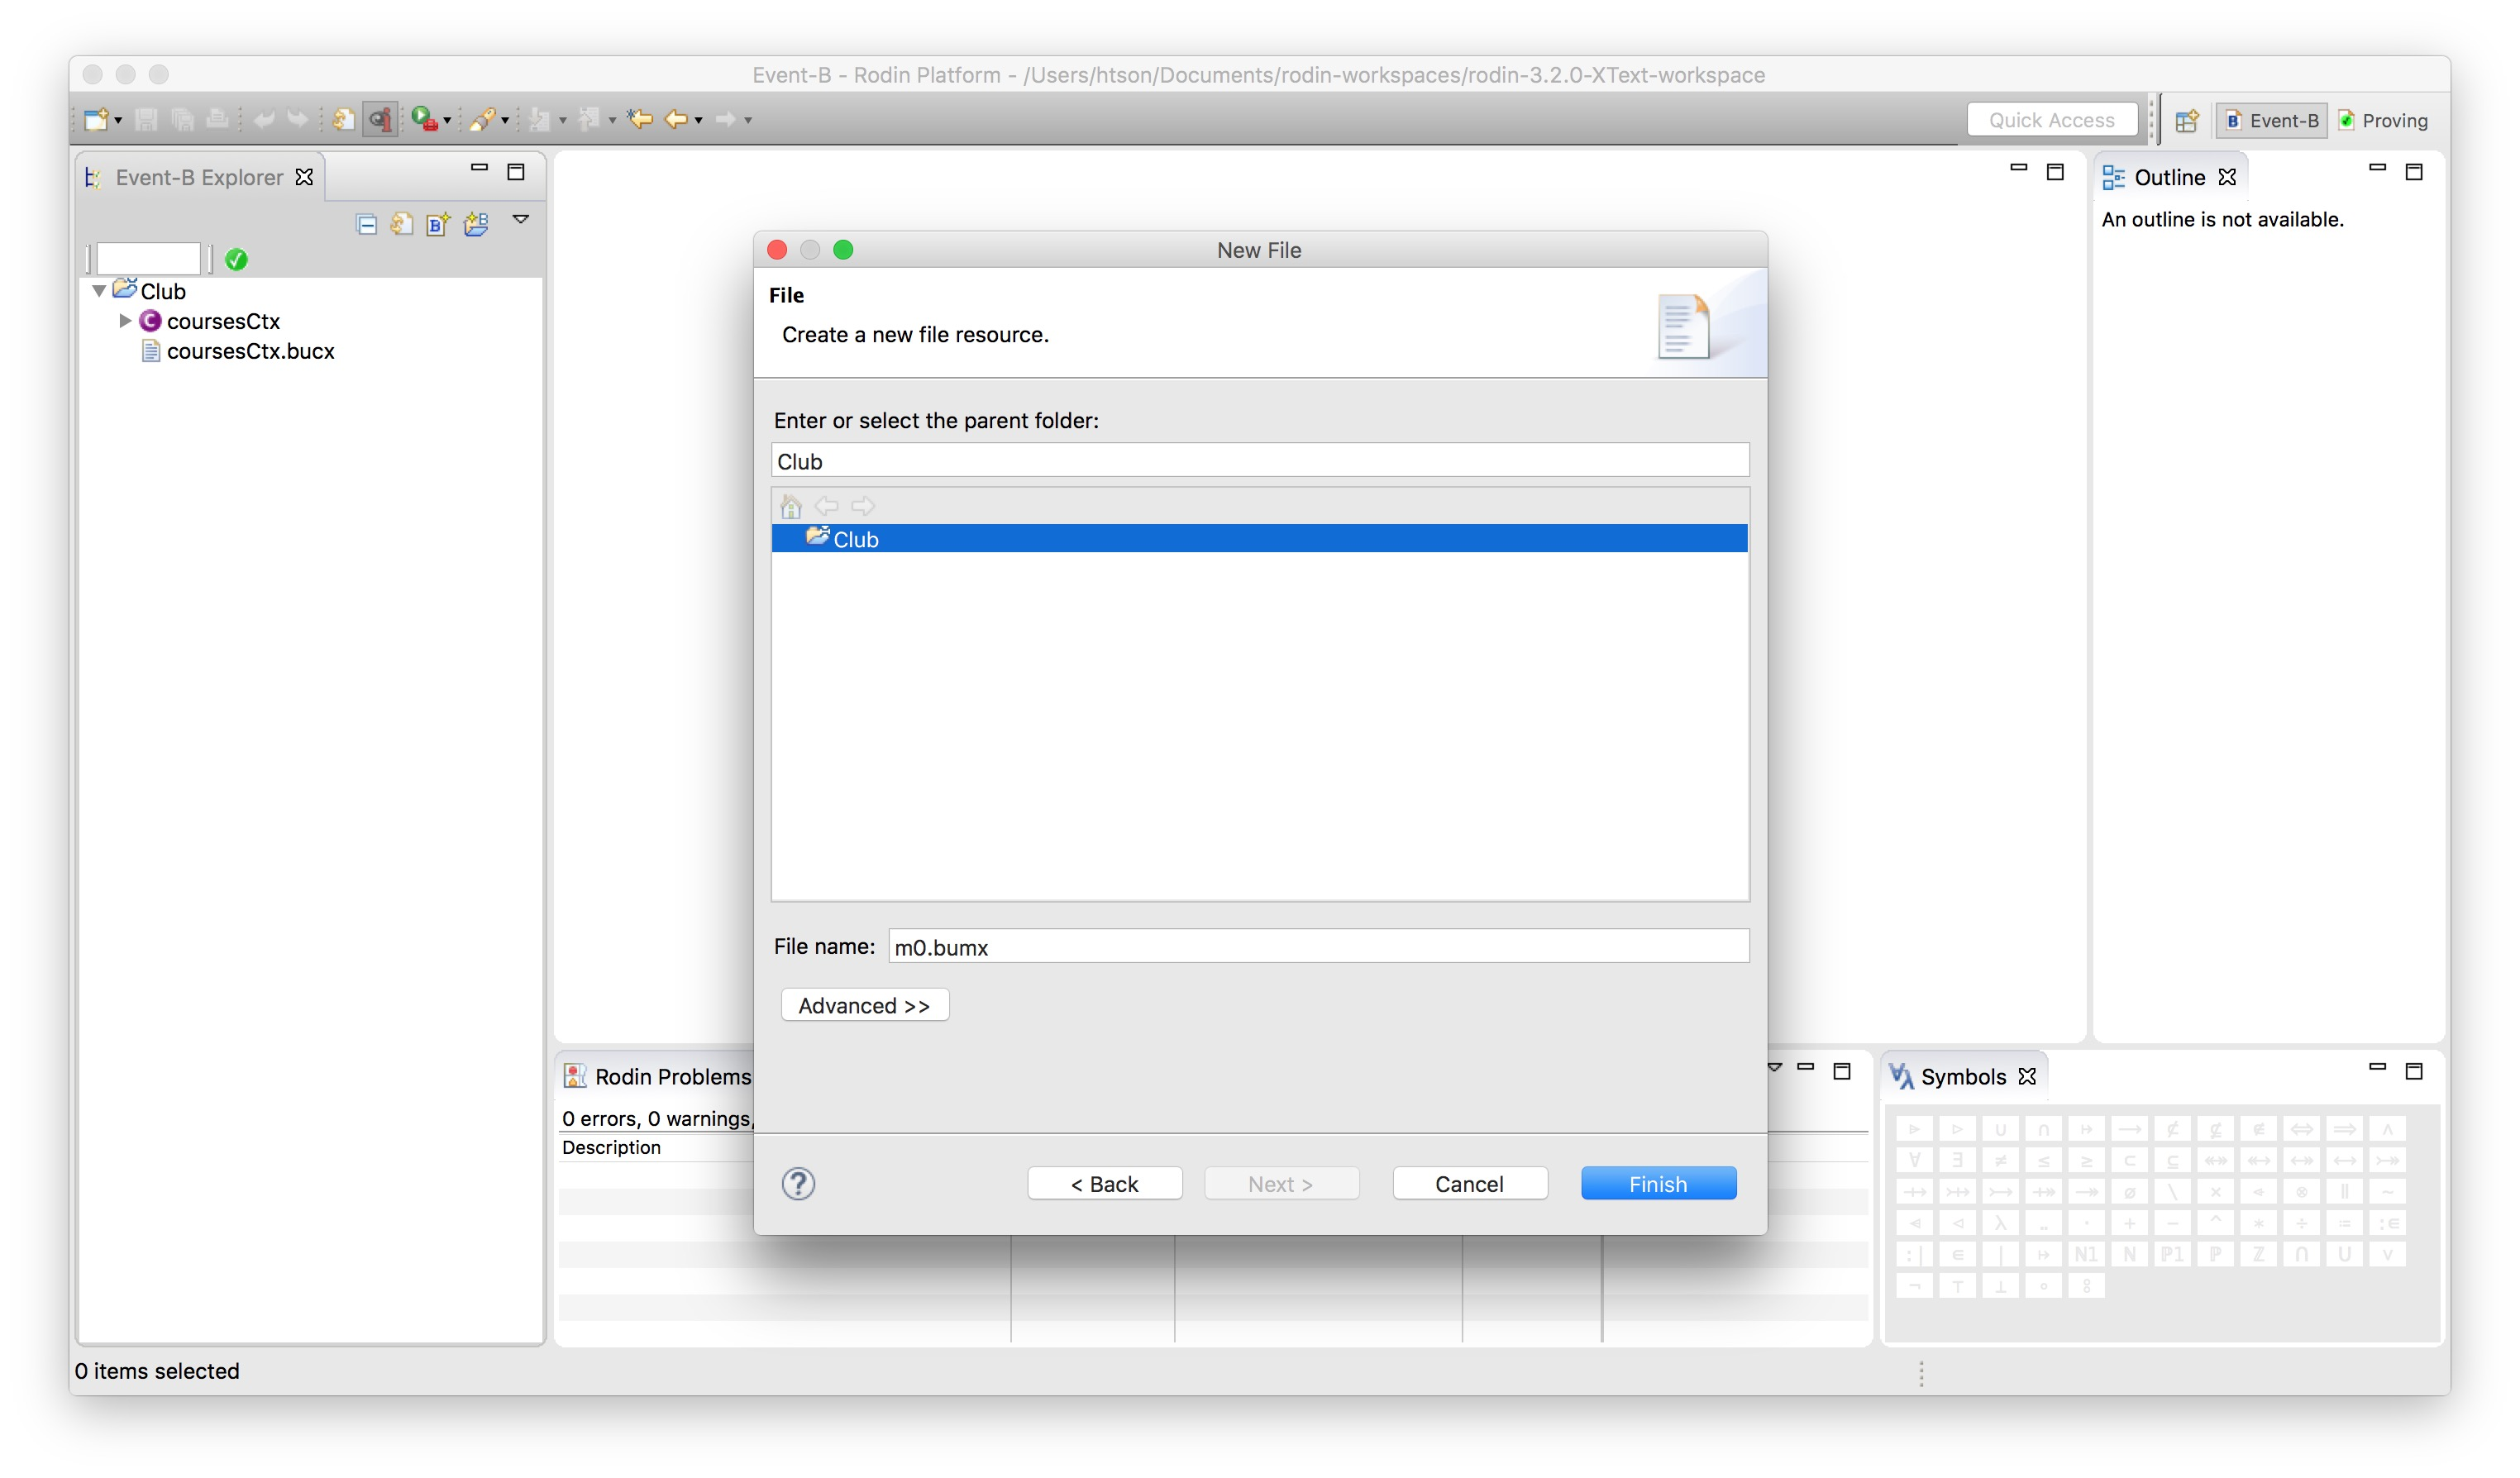
\includegraphics[width=512]{figures/CreateM0}
    \else
    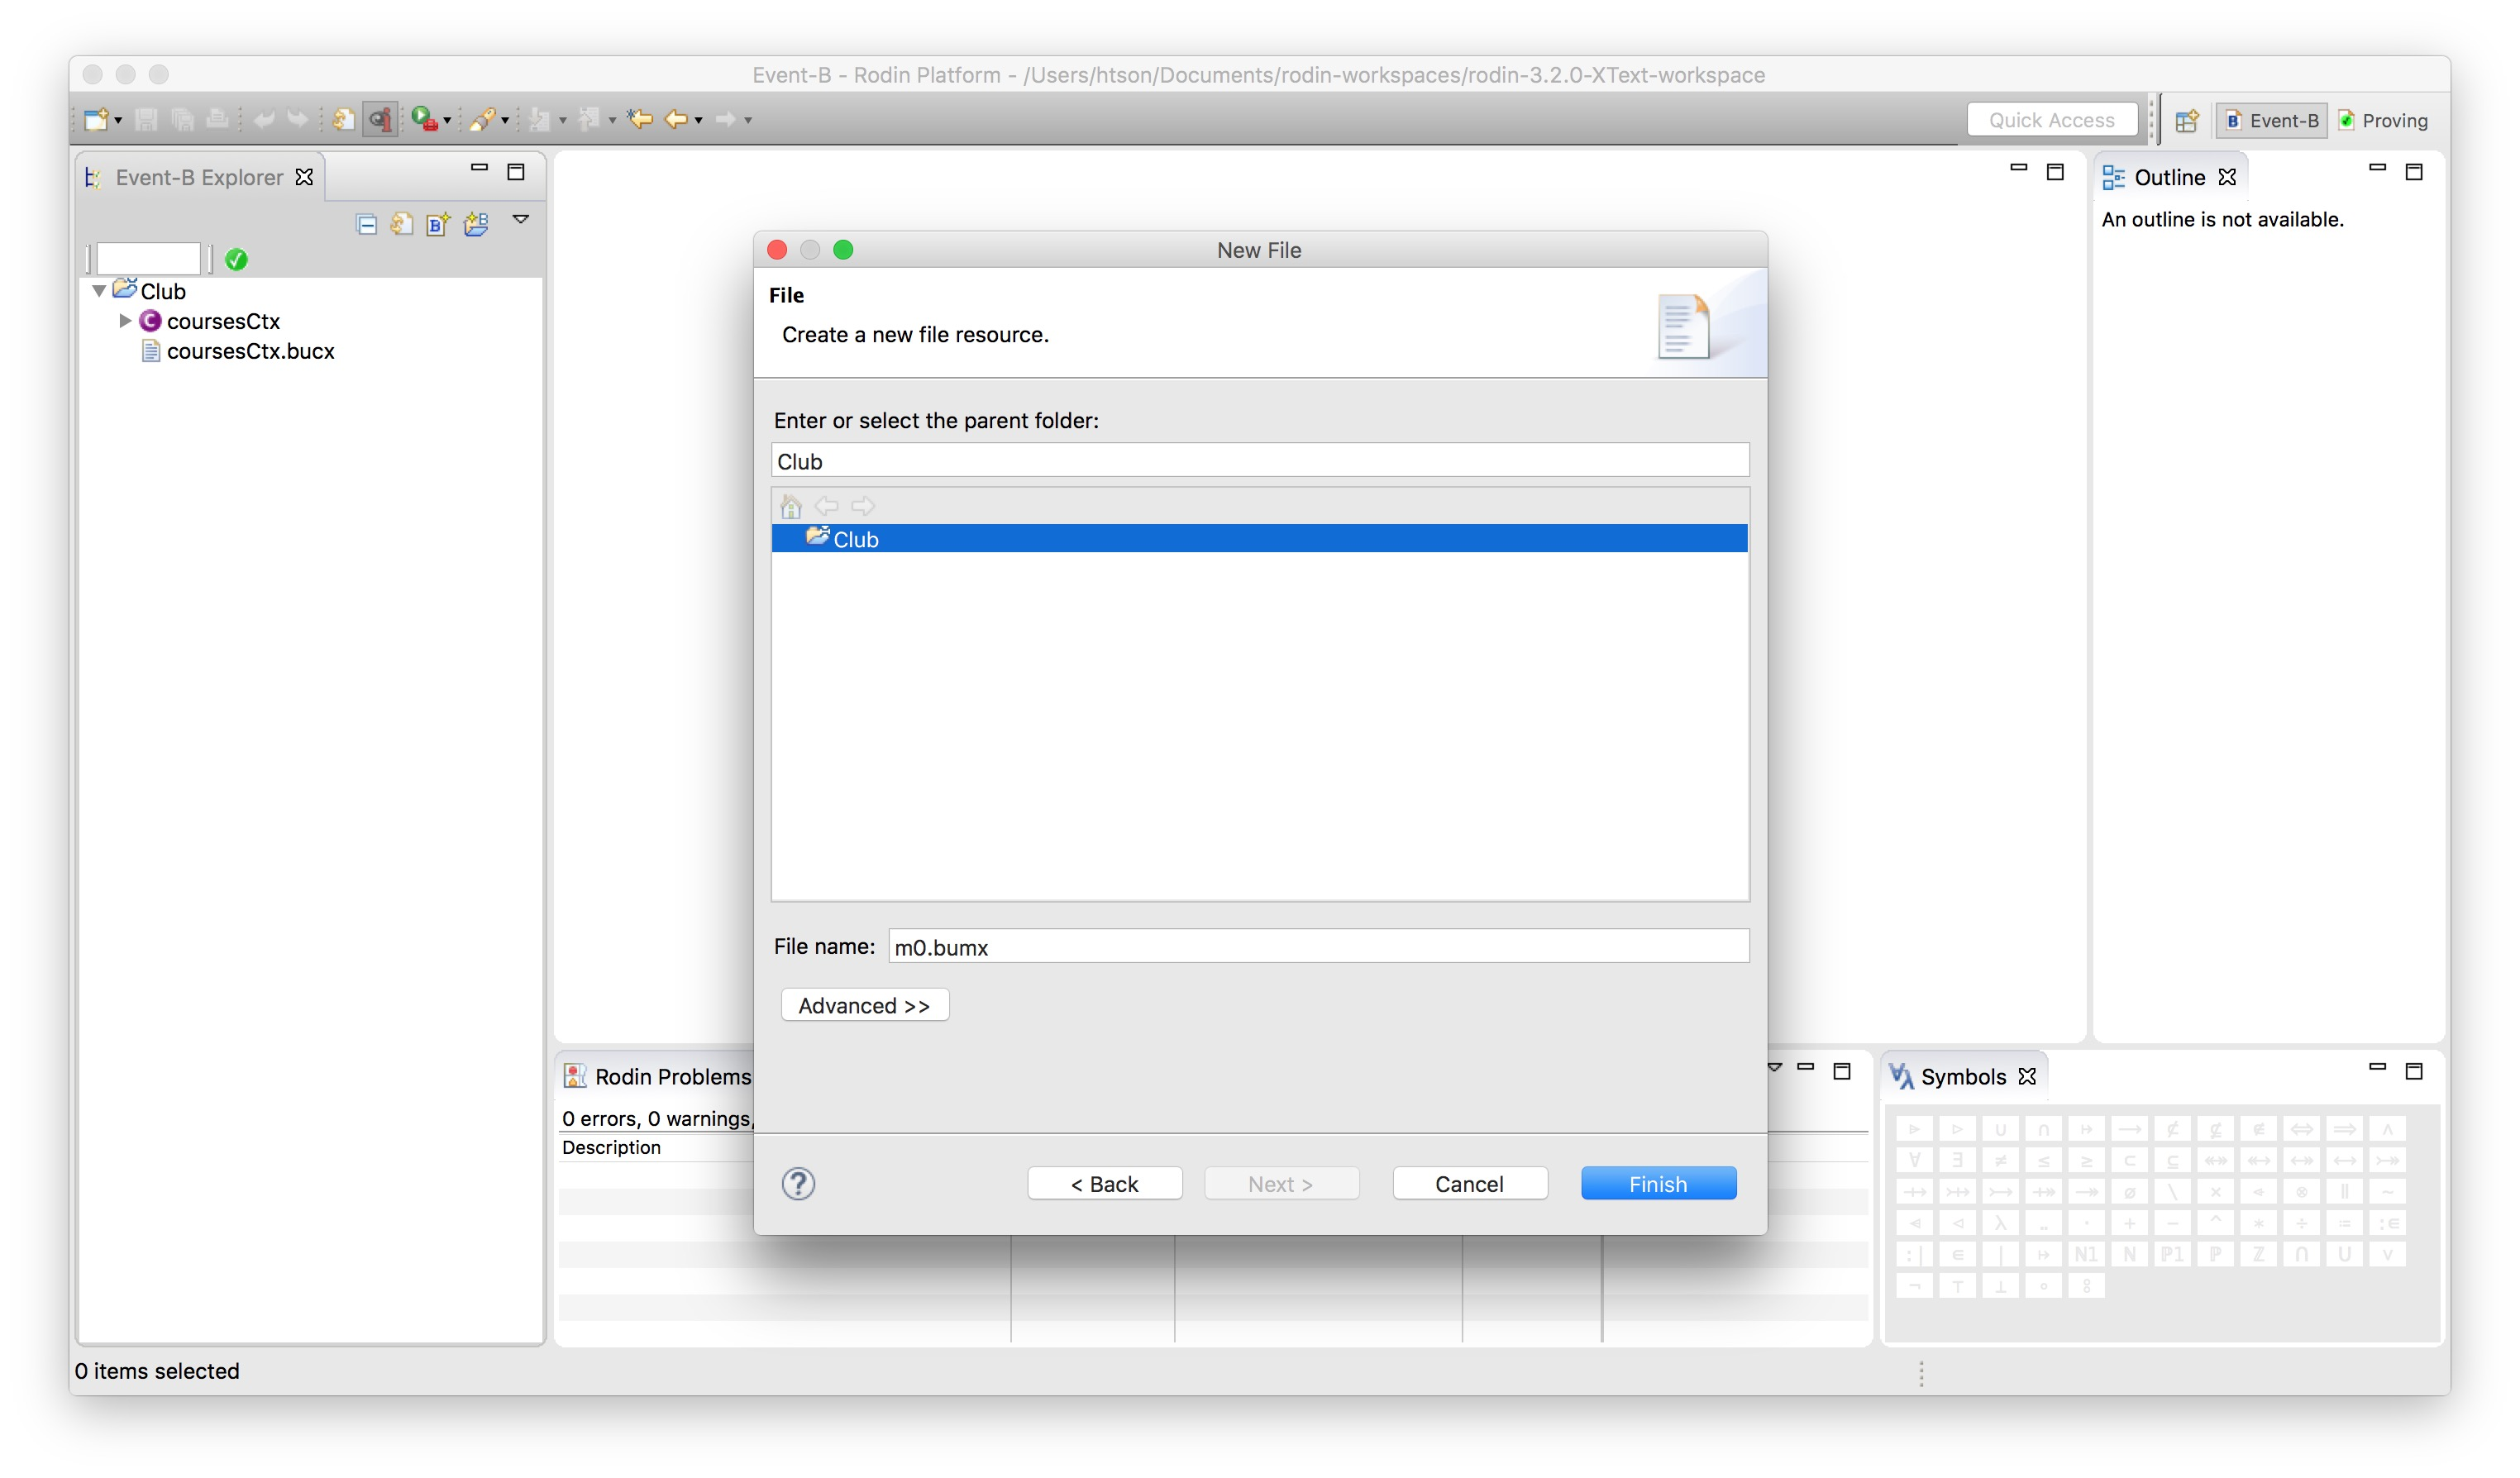
\includegraphics[width=0.9\textwidth]{figures/CreateM0}
    \fi
    \caption{Type-setting \ifplastex ℕ1 \else $\natn$ \fi using Content Assist}
    \label{fig:CreateM0}
  \end{figure}

\item[Step 2. Set the content of m0.bumx] \textbf{Set the content of "m0.bumx" as follows}.
  \begin{center}
    \begin{Bcode}
      \ifplastex
      \Bmachine{} m0 \\
      \Bvariables{} crs \\
      \Binvariants \\
      @inv0_1: "crs ∈ ℙ(CRS)"\\
      @thm0_2: "finite(crs)" \Btheorem \\
      @inv0_2: "card(crs) ≤ m" \\
      @DLF: "(card(crs) ≠ m) ∨ (∃cs·cs ⊆ crs ∧ cs ≠ ∅)" \\
      \Bevents\\
      INITIALISATION\\
      \Bbegin \\
      @act0_1: "crs ≔ ∅"\\
      \Bend\\
      OpenCourses\\
      \Bwhen\\
      @grd0_1: "card(crs) ≠ m" \\
      @thm0_3: "crs ≠ CRS" \Btheorem \\
      \Bthen\\
      @act0_1: "crs :∣ crs ⊂ crs' ∧ card(crs') ≤ m"\\
      \Bend\\
      CloseCourses \Banticipated\\
      \Bany{} cs \Bwhere\\
      @grd0_1: "cs ⊆ crs"\\
      @grd0_2: "cs ≠ ∅"\\
      \Bthen\\
      @act0_1: "crs ≔ crs ∖ cs"\\
      \Bend\\
      \Bend
      \else
      \Bmachine{} m0 \\
      \Bvariables{} crs \\
      \Binvariants \\
      \Btab @inv0\_1: "\(crs \in \pow(CRS)\)"\\
      \Btab @thm0\_2: "\(\finite(crs)\)" \Btheorem \\
      \Btab @inv0\_2: "\(\card(crs) \leq m\)" \\
      \Btab @DLF: "\((\card(crs) \neq m) \lor (\exists cs \qdot cs \subseteq crs \land cs \neq \emptyset)\)" \\
      \Bevents\\
      \Btab INITIALISATION\\
      \Btab \Bbegin \\
      \Btab\Btab @act0\_1: "\(crs \bcmeq \emptyset\)"\\
      \Btab \Bend\\
      \Btab OpenCourses\\
      \Btab \Bwhen\\
      \Btab \Btab @grd0\_1: "\(\card(crs) \neq m\)" \\
      \Btab \Btab @thm0\_3: "\(crs \neq CRS\)" \Btheorem \\
      \Btab \Bthen\\
      \Btab \Btab @act0\_1: "\(crs \bcmsuch crs \subset crs' \land \card(crs') \leq m\)"\\
      \Btab \Bend\\
      \Btab CloseCourses \Banticipated\\
      \Btab \Bany{} cs \Bwhere\\
      \Btab \Btab @grd0\_1: "\(cs \subseteq crs\)"\\
      \Btab \Btab @grd0\_2: "\(cs \neq \emptyset\)"\\
      \Btab \Bthen\\
      \Btab \Btab @act0\_1: "\(crs \bcmeq crs \setminus cs\)"\\
      \Btab \Bend\\
      \Bend
      \fi
    \end{Bcode}
  \end{center}
\item[Step 3. Auto-format the code] \textbf{Automatically format the content of ``m0.bumx''} by using short-cut (e.g., on Mac OS: Cmd+Shift+F).

\item[Step 4. Save the file] \textbf{Save the file ``m0.bumx''}.

\item[Step 5. Add missing ``sees'' clause] In the compiled Rodin Machine m0, there are several errors, due to the fact that \textbf{m0} refers to the sets and constants of the context courseCtx.
  \textbf{Add the missing ``sees'' clause} after the ``machine'' clause
  \begin{center}
    \begin{Bcode}
      \Bsees{} courseCtx
    \end{Bcode}
  \end{center}
  (Note: One can use \emph{Content Assist} after typing the ``sees'' keyword to select the context, see Figure~\ref{fig:SeesCoursesCtx}).
  \begin{figure}[!htbp]
    \centering
    \ifplastex
    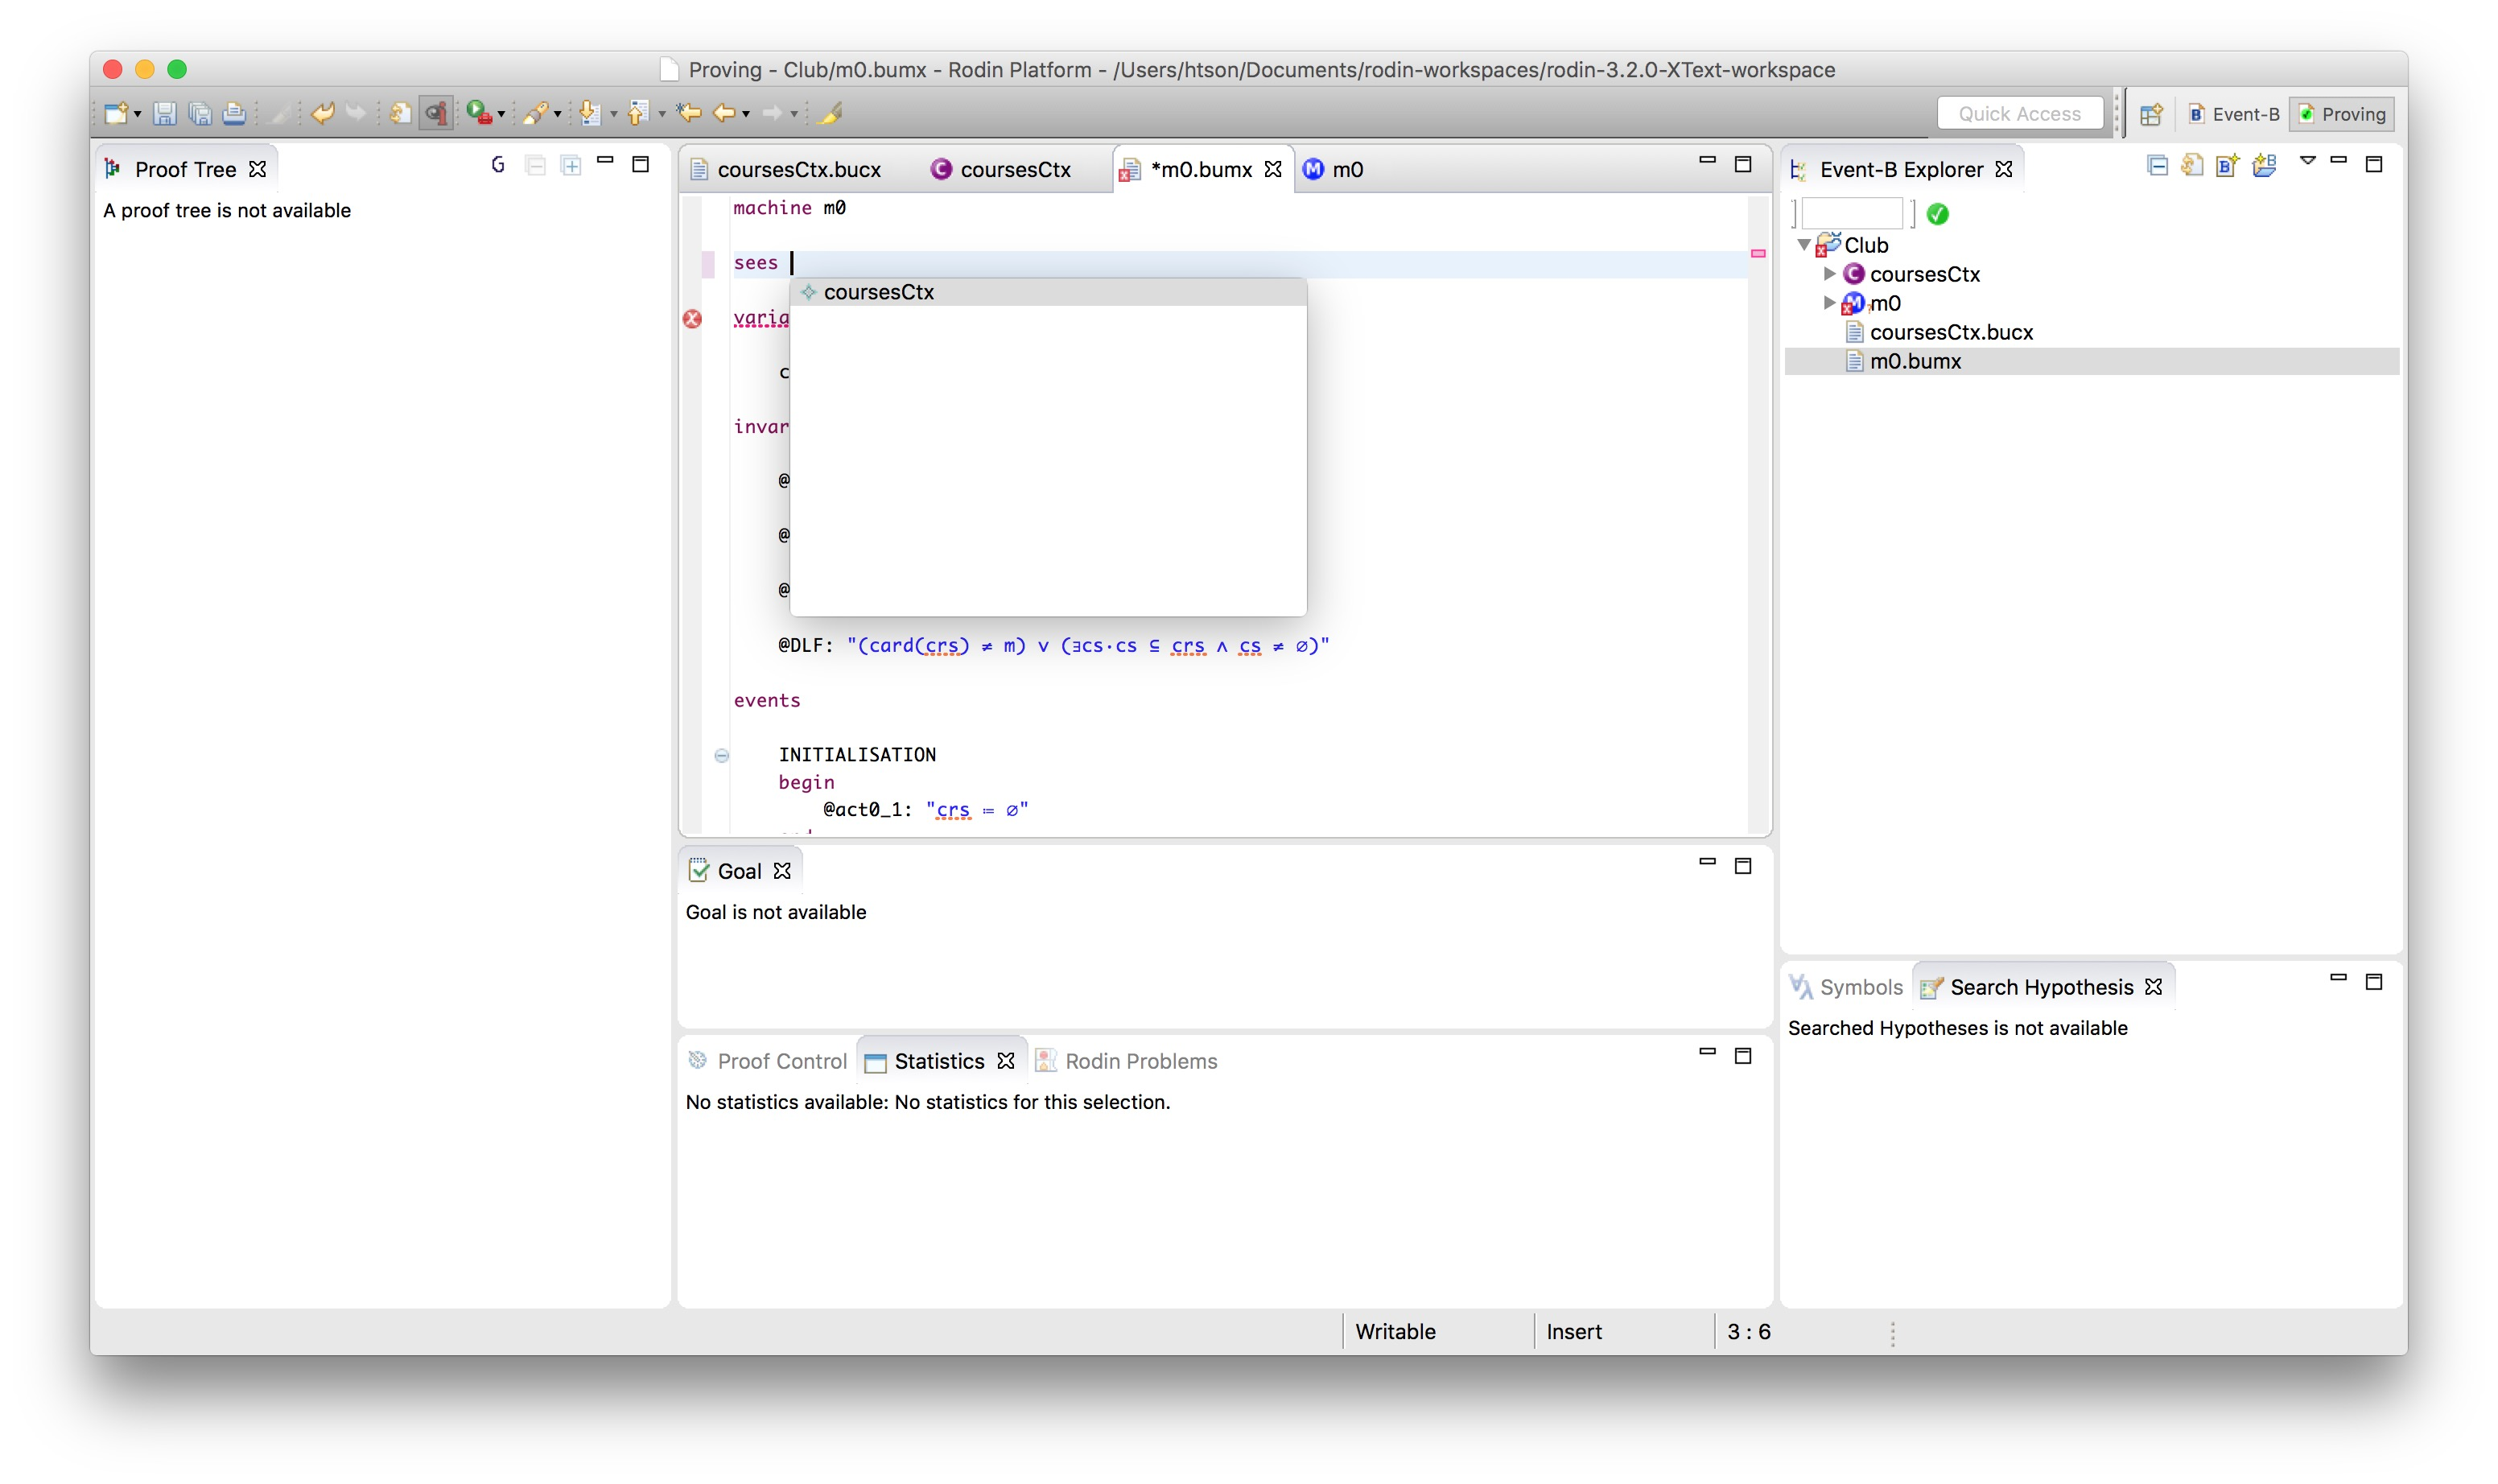
\includegraphics[width=512]{figures/SeesCoursesCtx}
    \else
    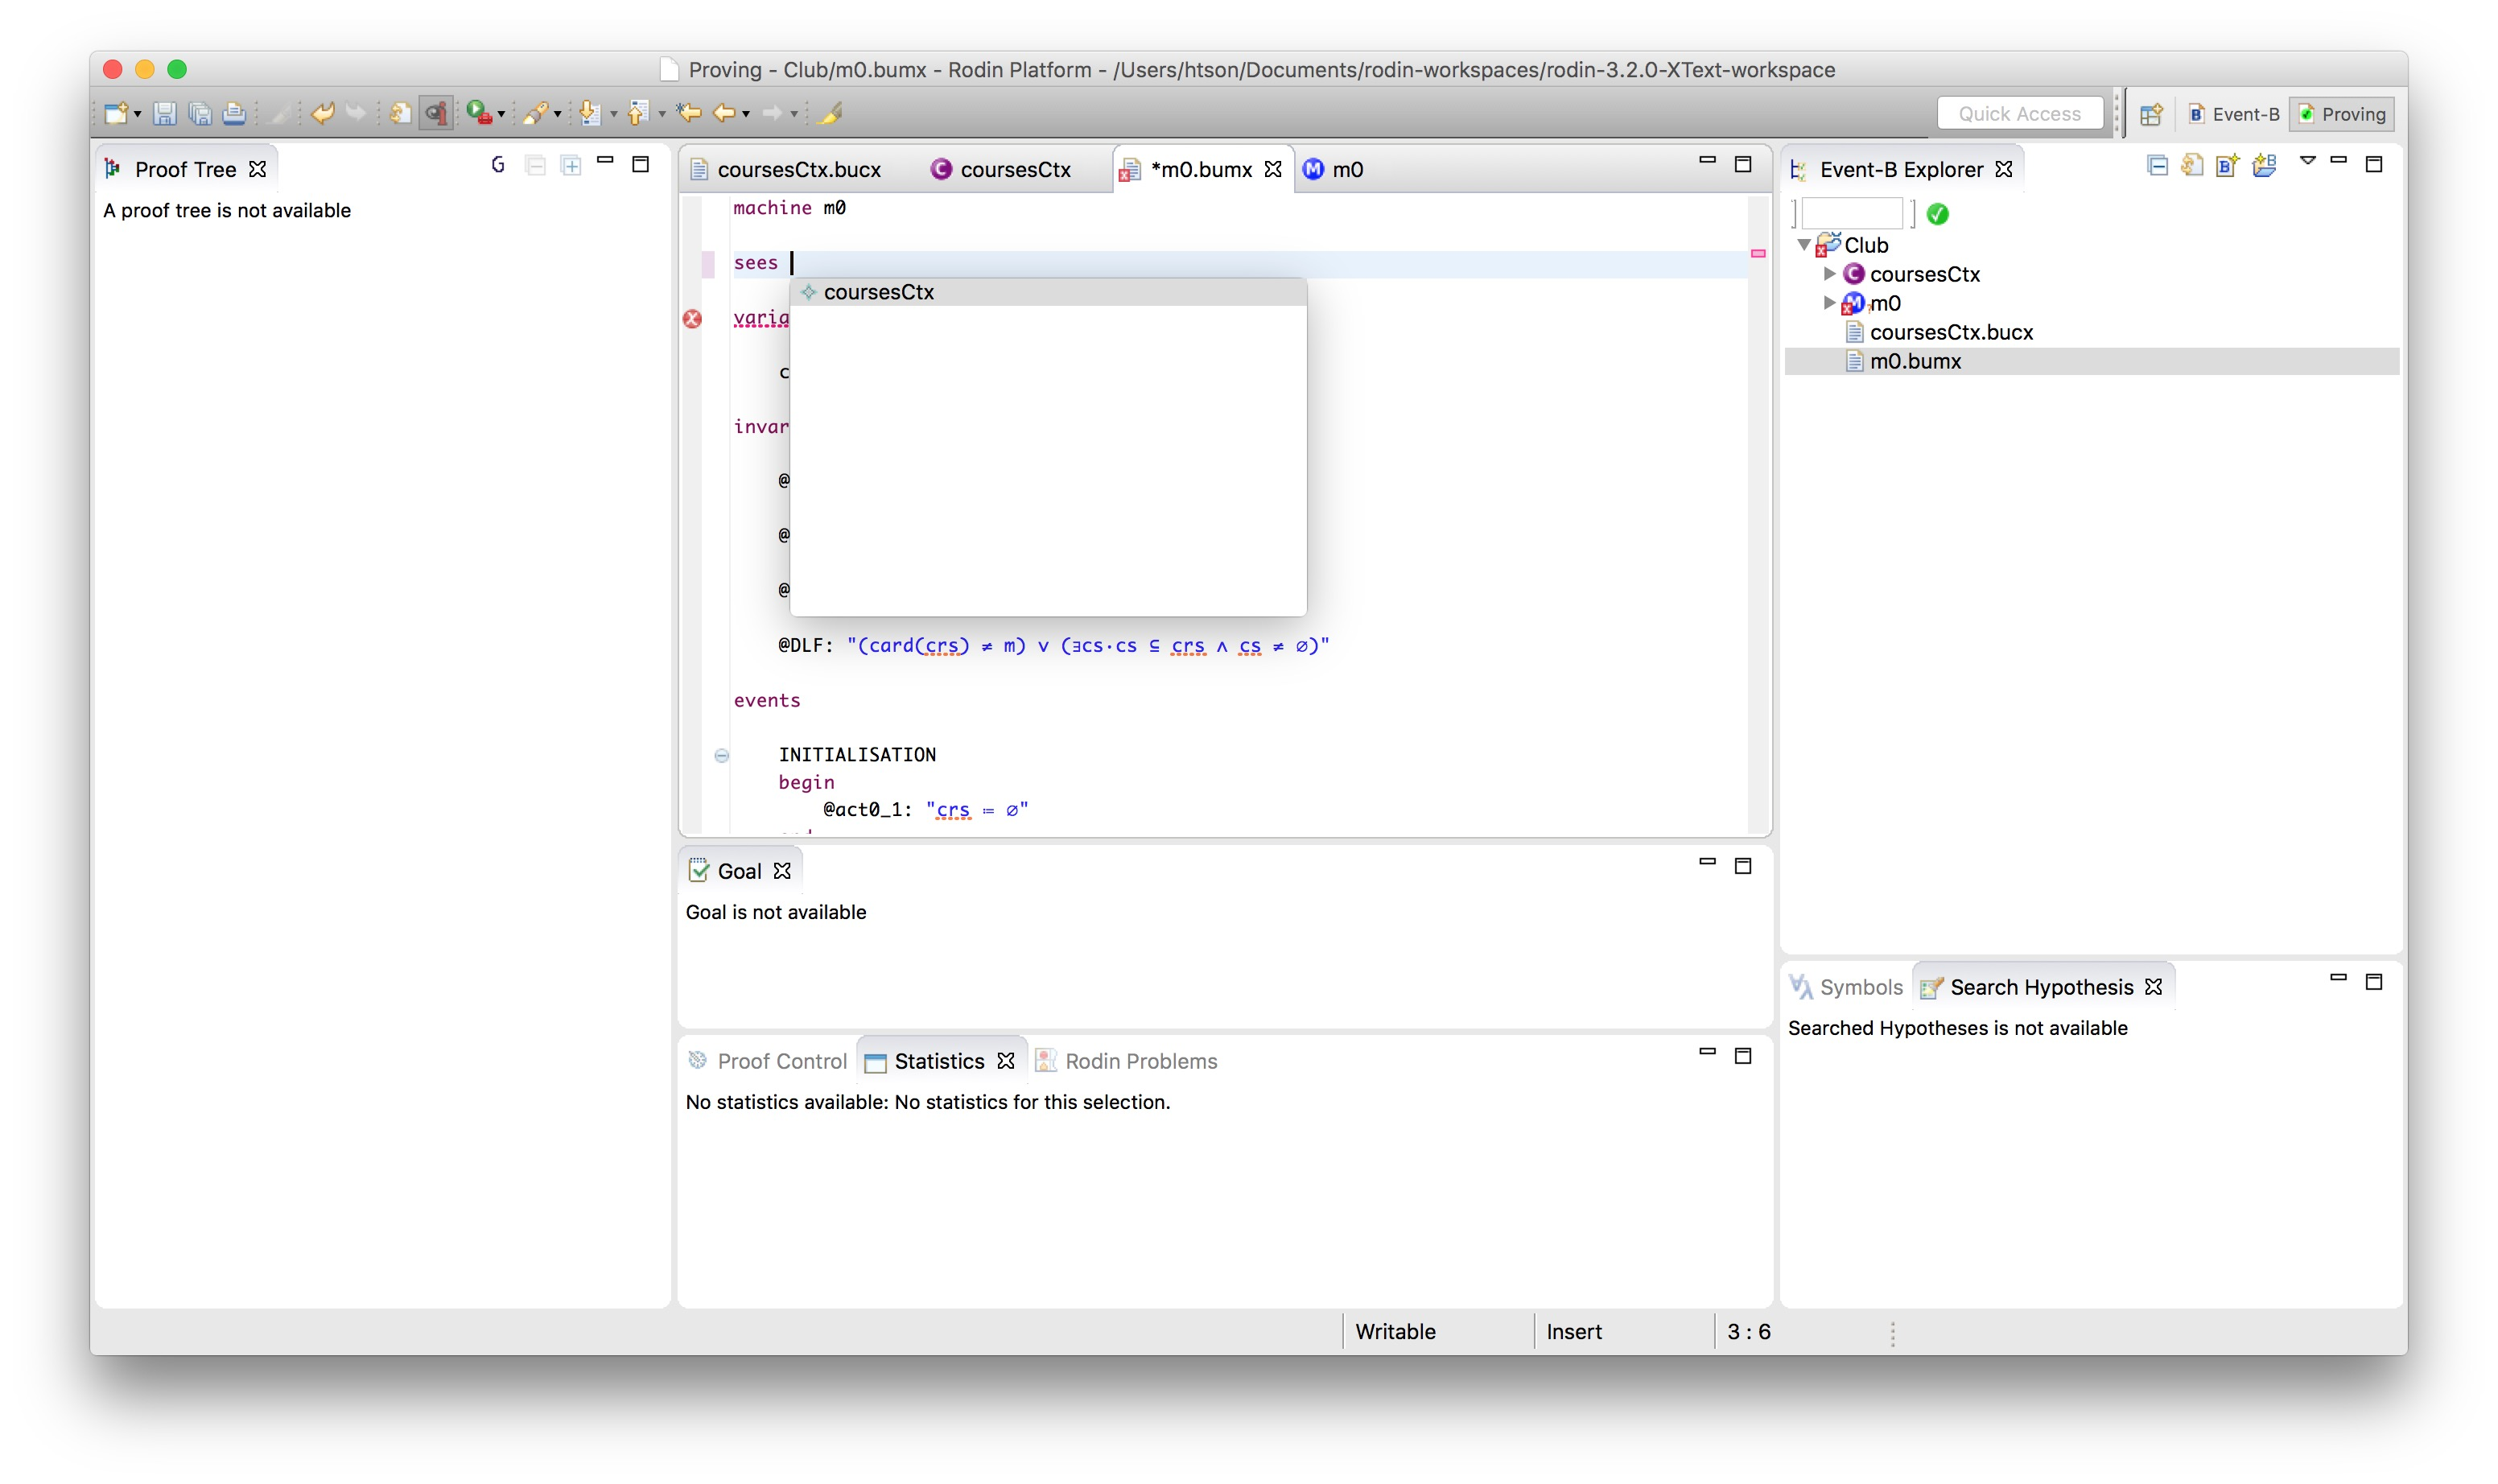
\includegraphics[width=0.9\textwidth]{figures/SeesCoursesCtx}
    \fi
    \caption{Content Assist for adding Sees clause}
    \label{fig:SeesCoursesCtx}
  \end{figure}

\item[Step 6. Save the file again] \textbf{Save the file "m0.bumx" again}.
\end{description}
\textbf{Conclusion} By now, the XMachine ``m0.bumx'' and the corresponding Rodin Machine ``m0'' (without any error) should be visible in the Event-B Explorer (see Figure~\ref{fig:M0}.
  \begin{figure}[!htbp]
    \centering
    \ifplastex
    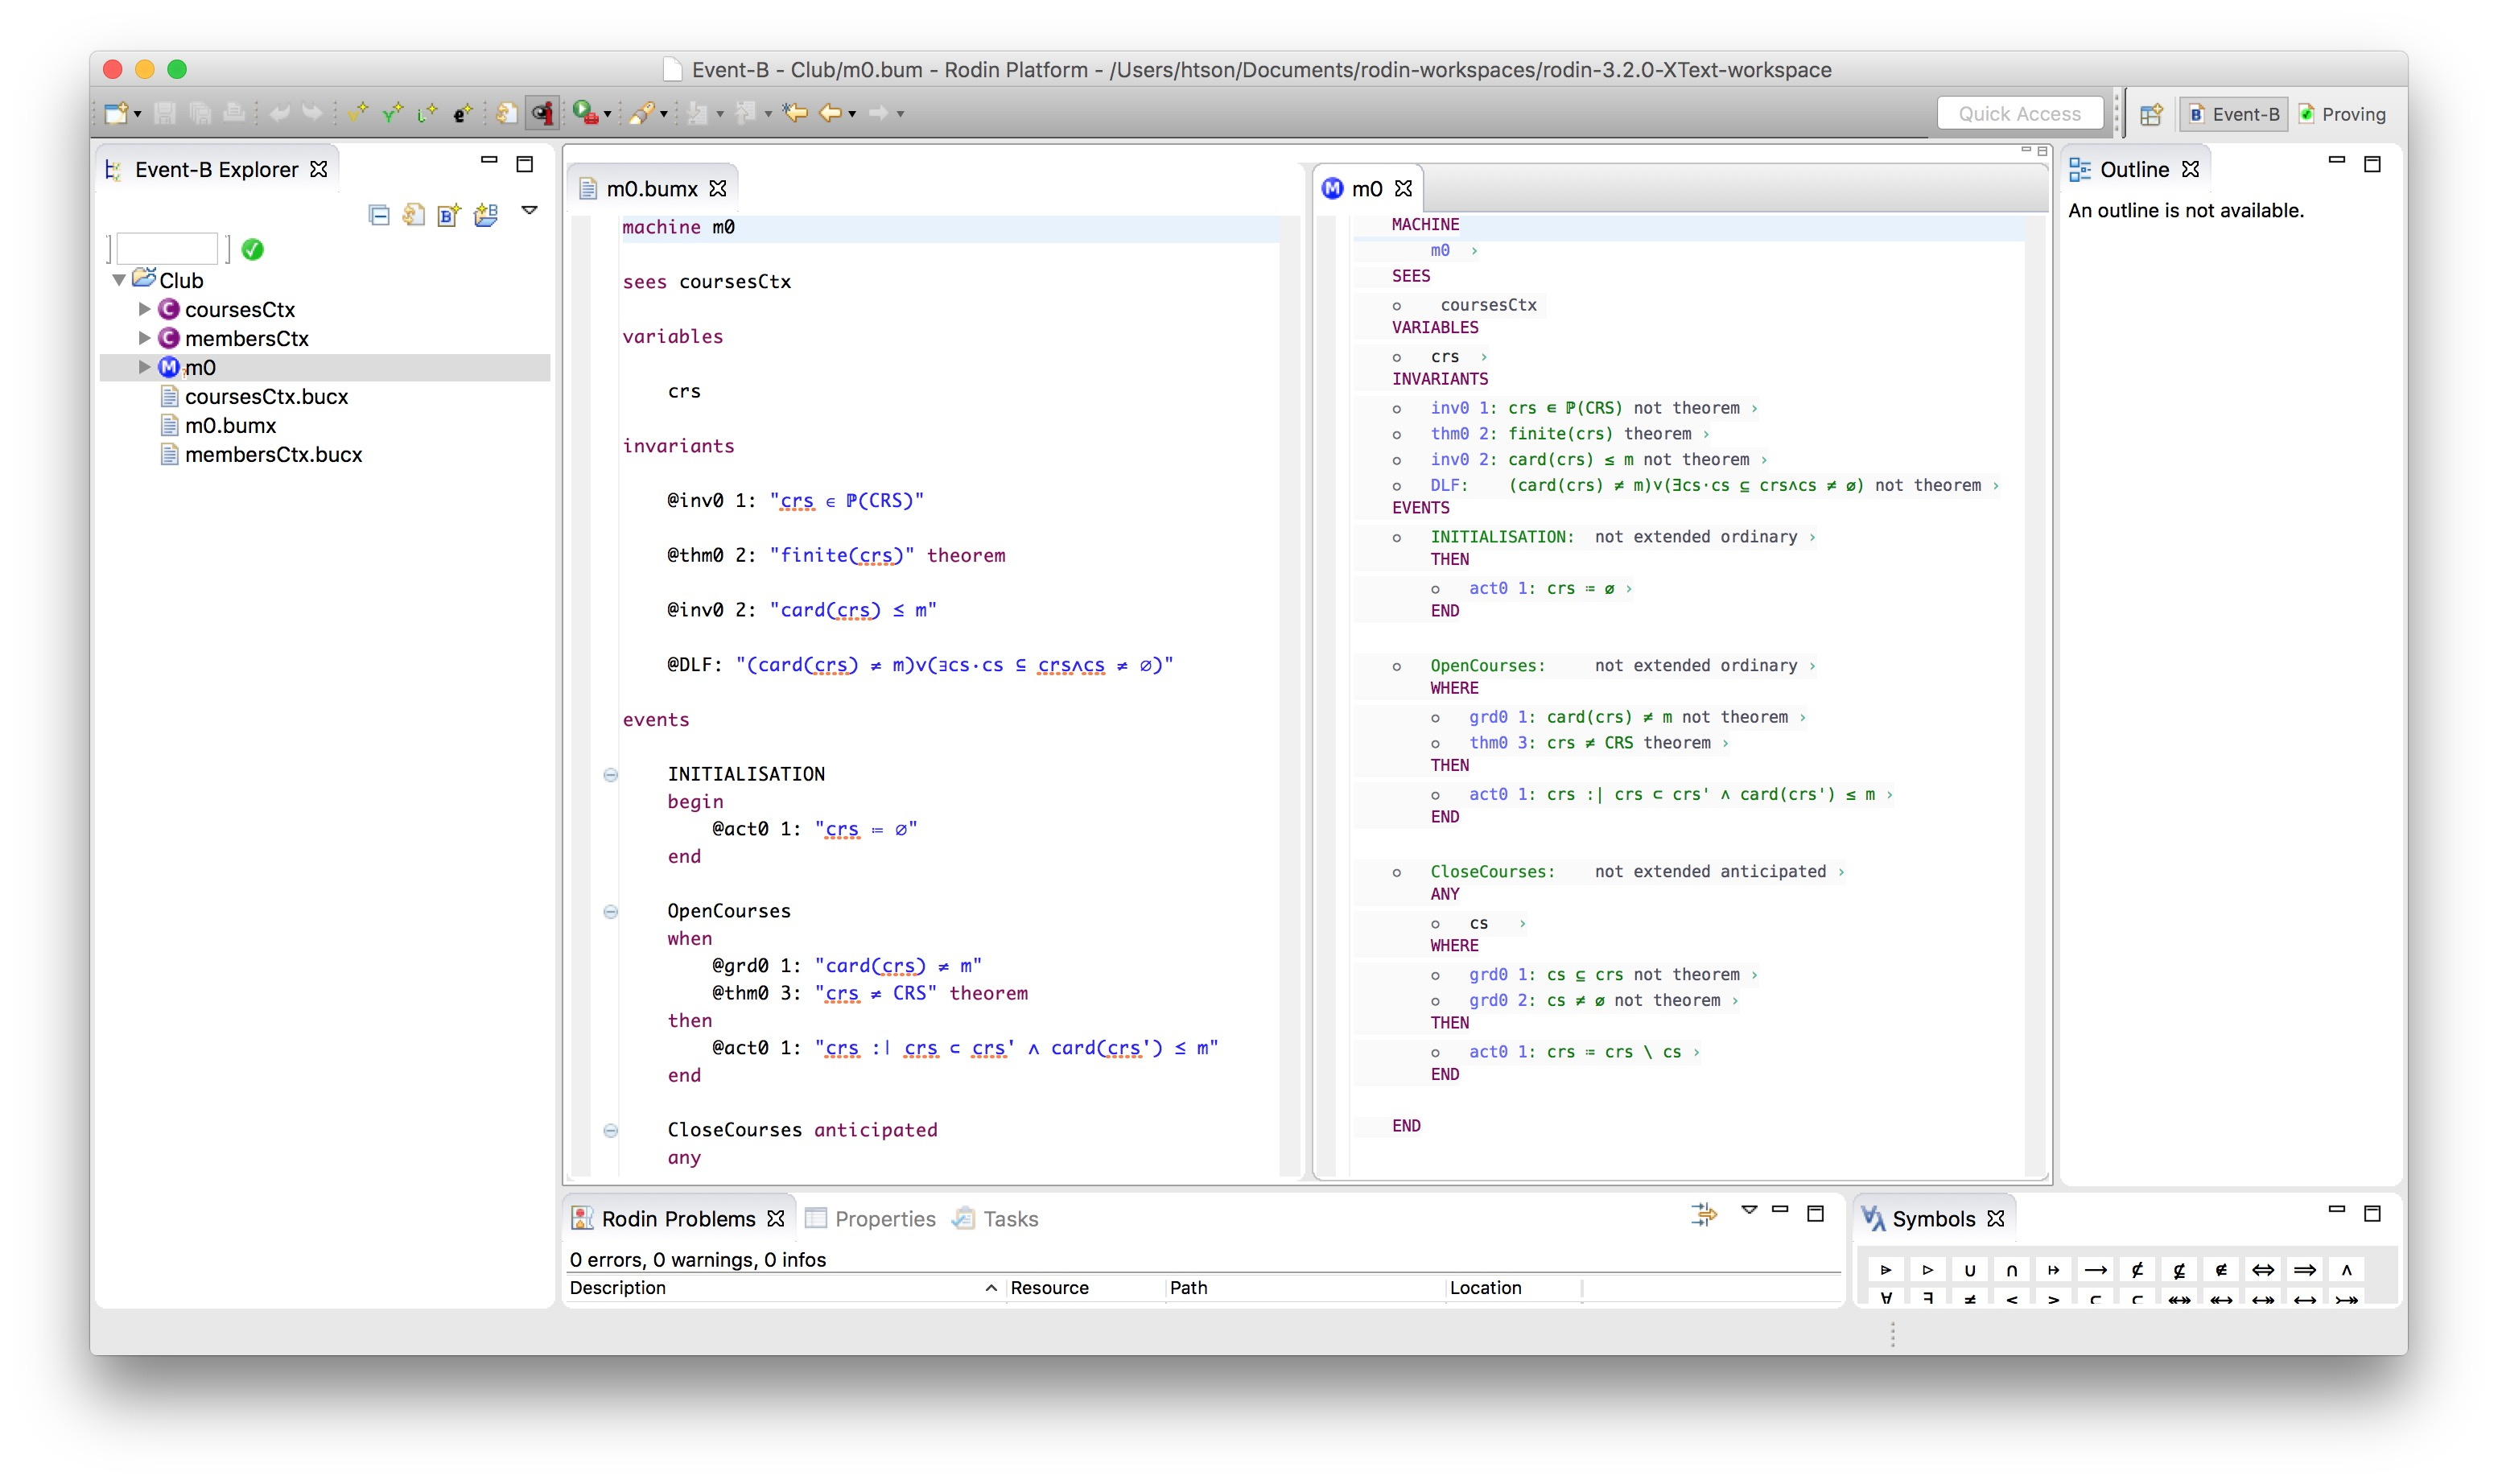
\includegraphics[width=512]{figures/M0}
    \else
    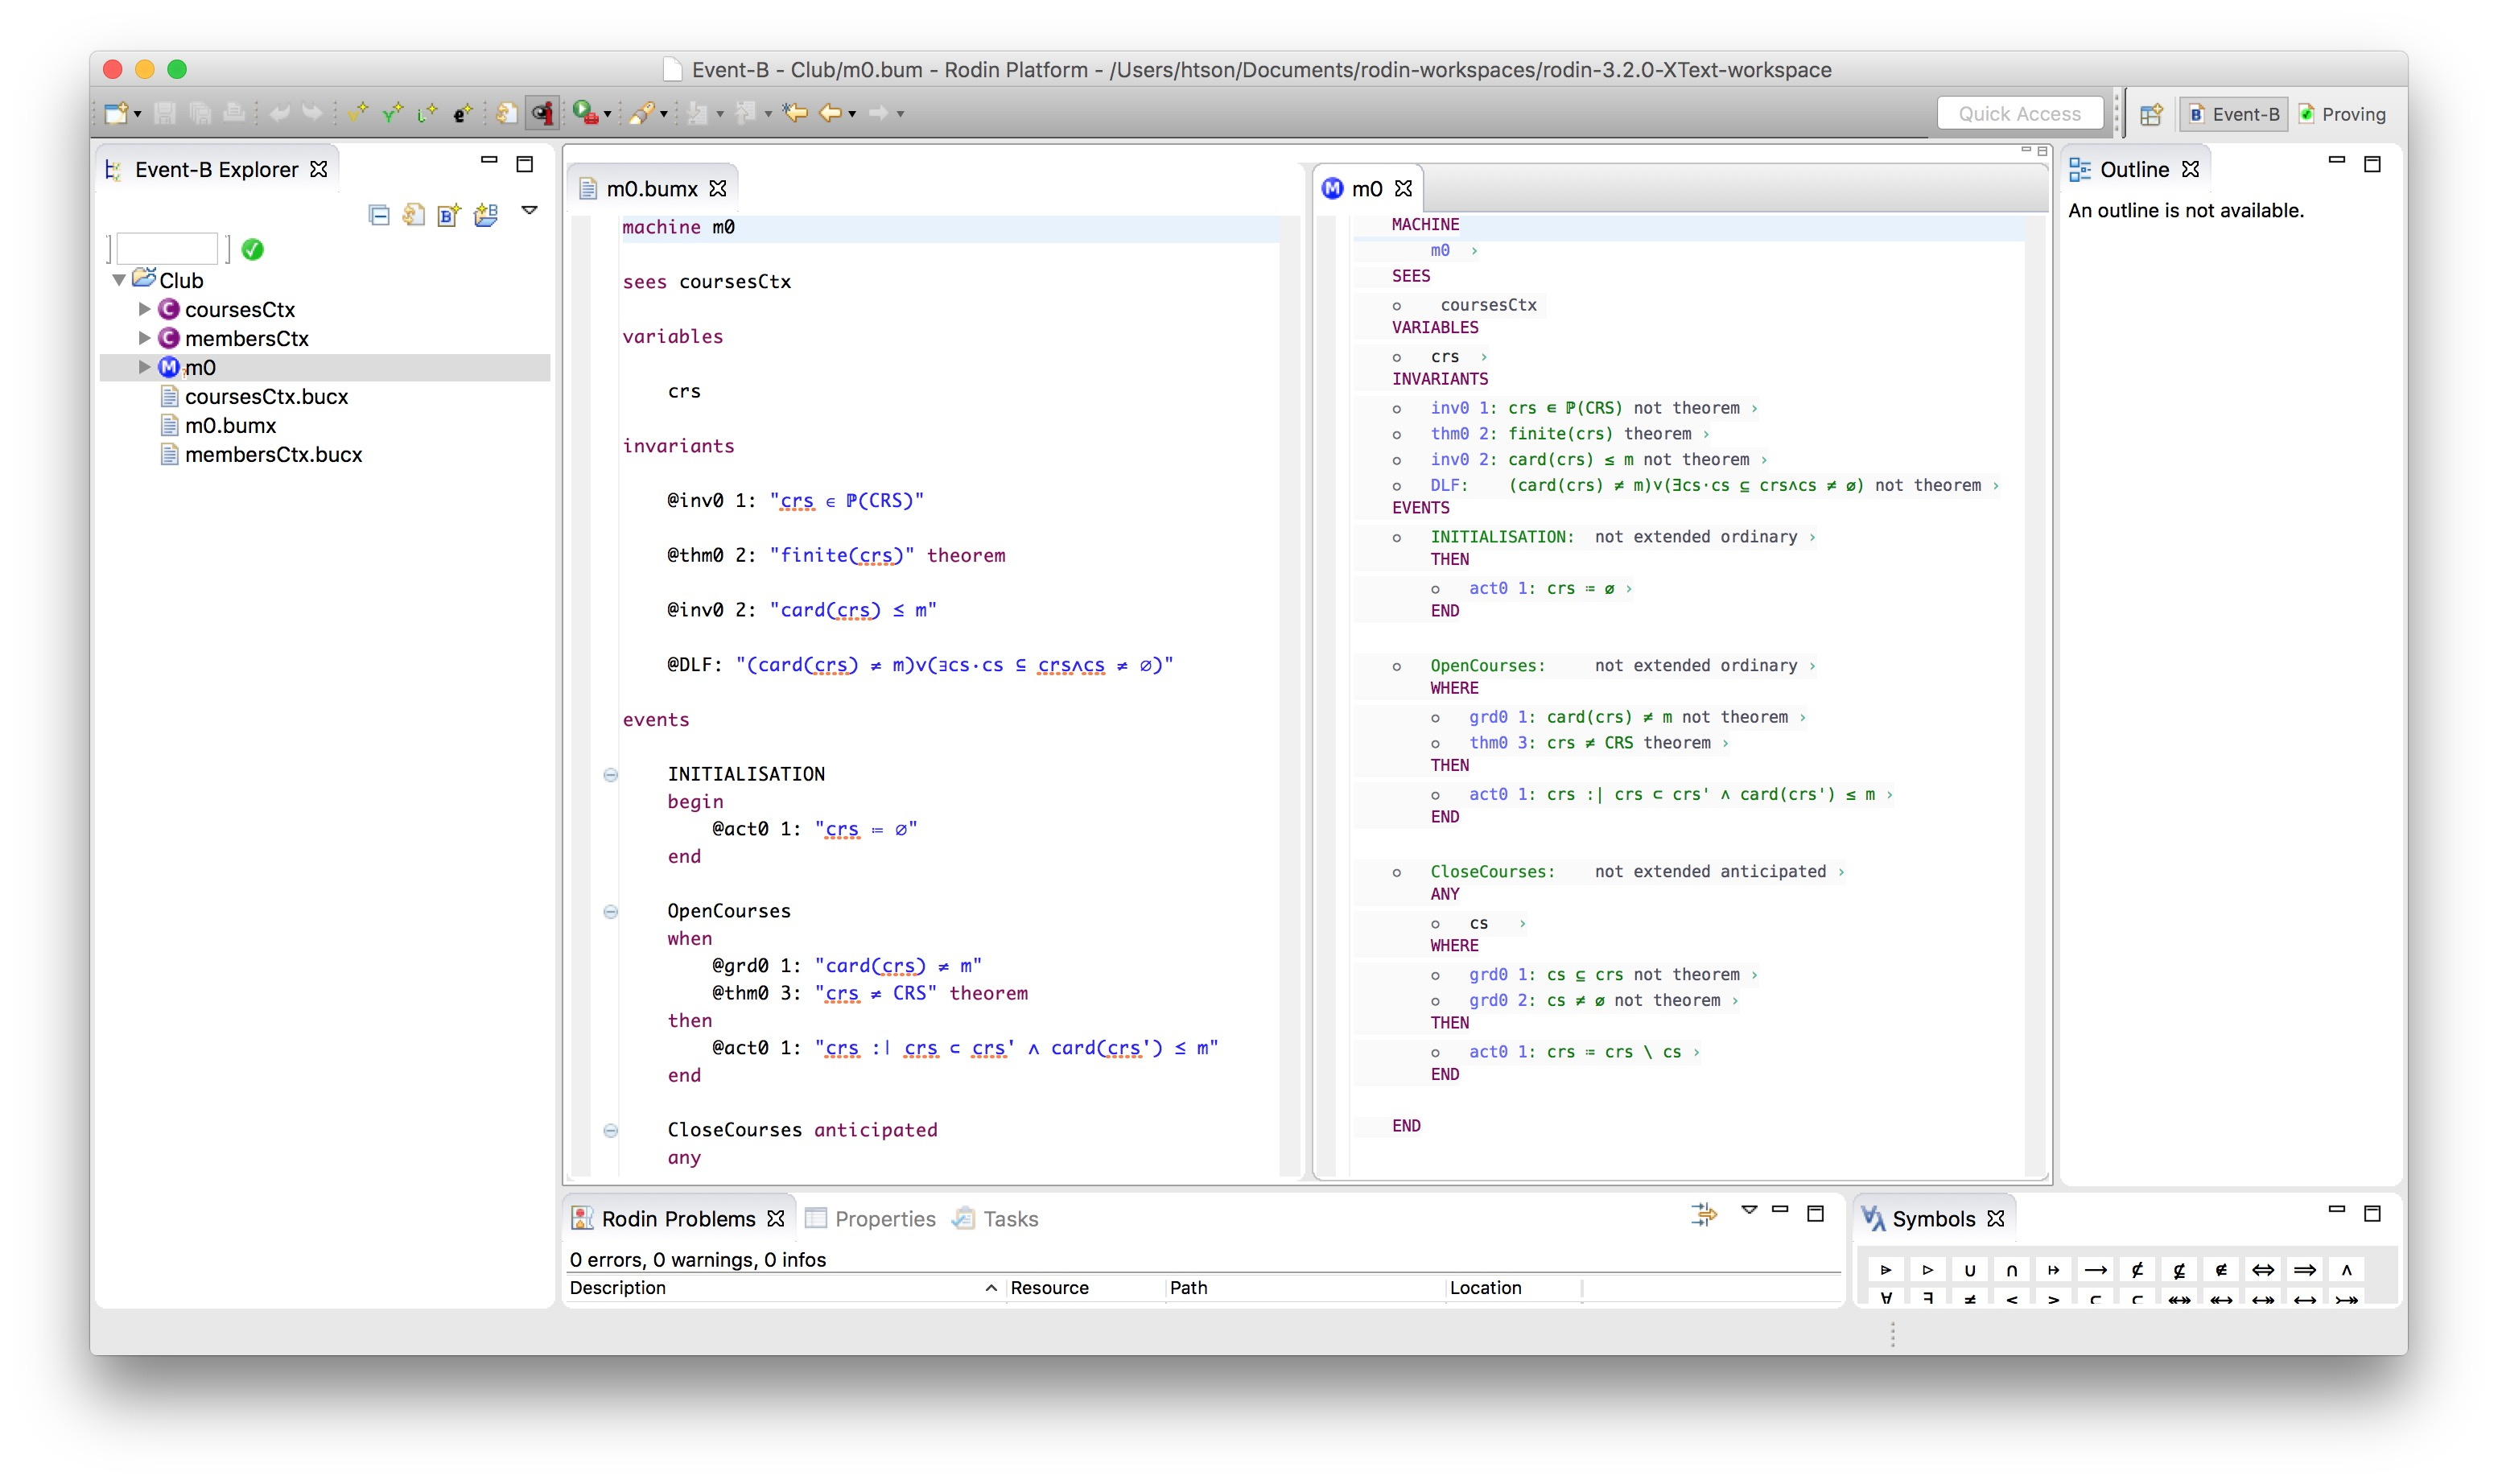
\includegraphics[width=0.9\textwidth]{figures/M0}
    \fi
    \caption{XMachine m0.bucx}
    \label{fig:M0}
  \end{figure}

\subsubsection{Task 5. Create extended XContexts}
\textbf{Introduction} The purpose of this task is to create some more extended XContexts within the "Club" project.

\paragraph{Task 5.1. Create a simple XContext membersCtx.bucx}
\textbf{Introduction} The purpose of this sub-task is to create a simple XContext ``membersCtx.bucx'' within the ``Club'' project.
\begin{description}
\item[Step 1. Create a new XContext membersCtx.bucx] \textbf{Create a new XContext} named ``membersCtx.bucx'' using the \emph{New File} wizard (see Figure~\ref{fig:CreateMembersCtx}.
  \begin{figure}[!htbp]
    \centering
    \ifplastex
    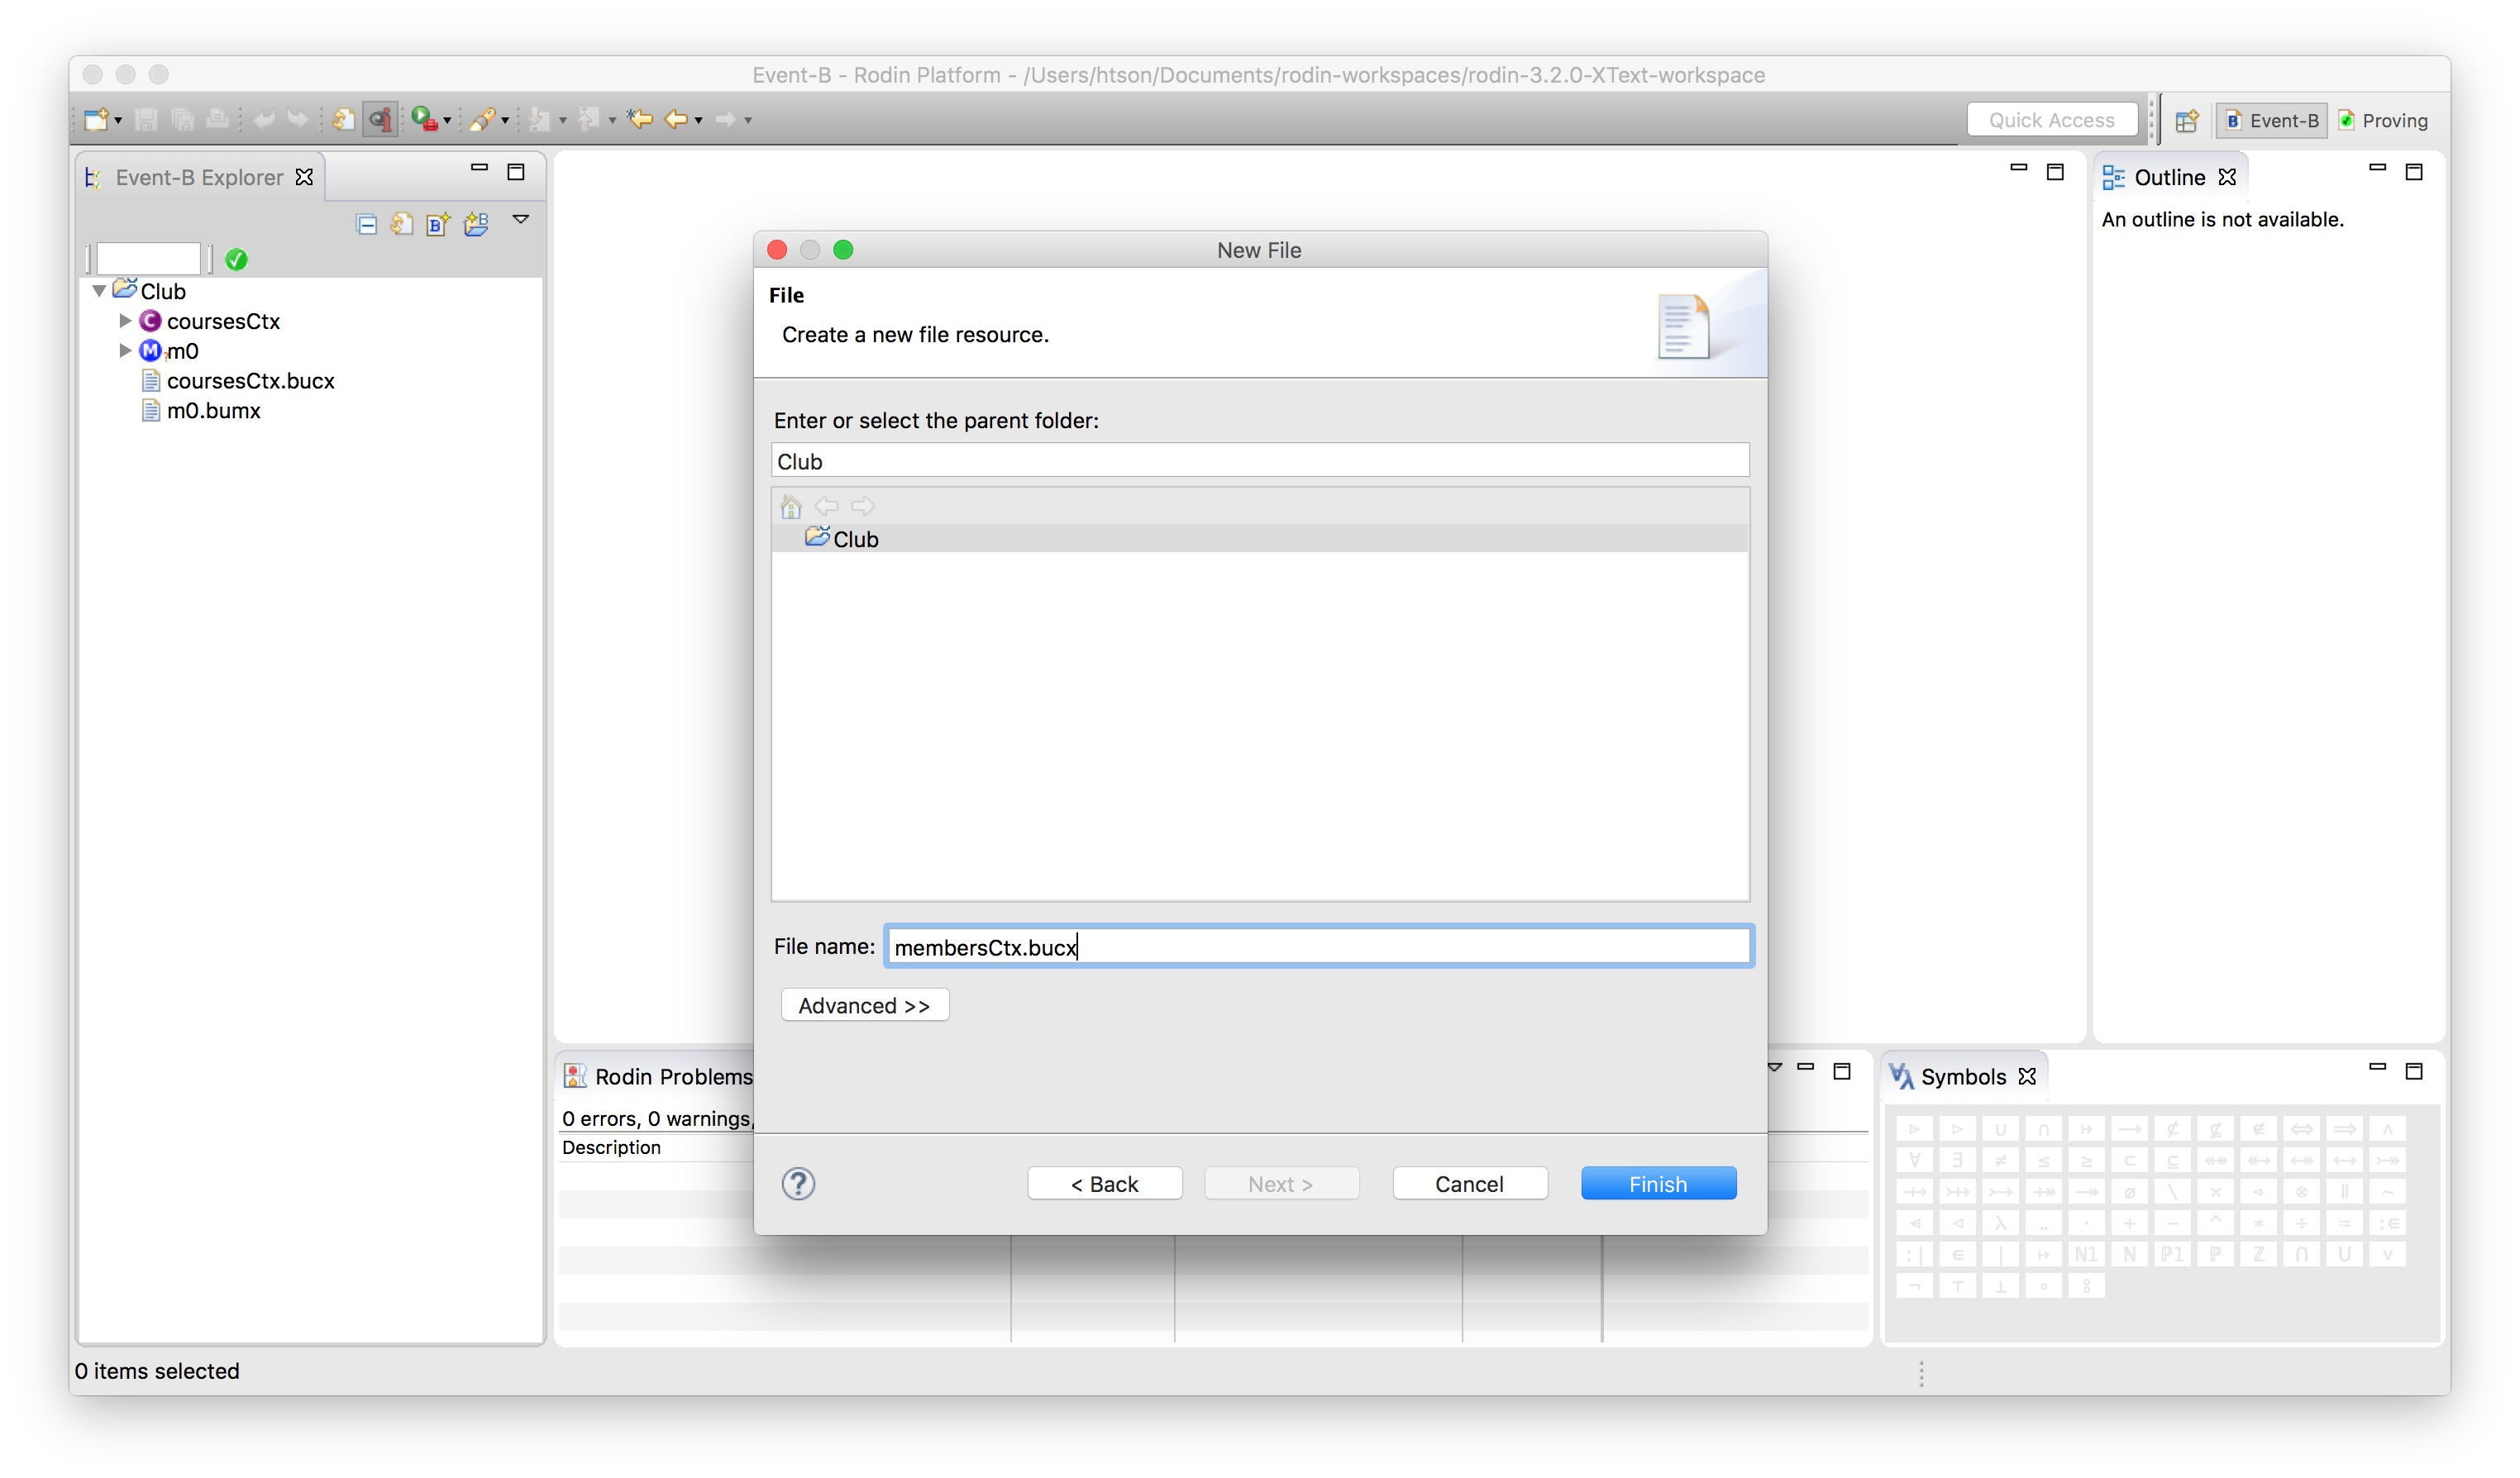
\includegraphics[width=512]{figures/CreateMembersCtx}
    \else
    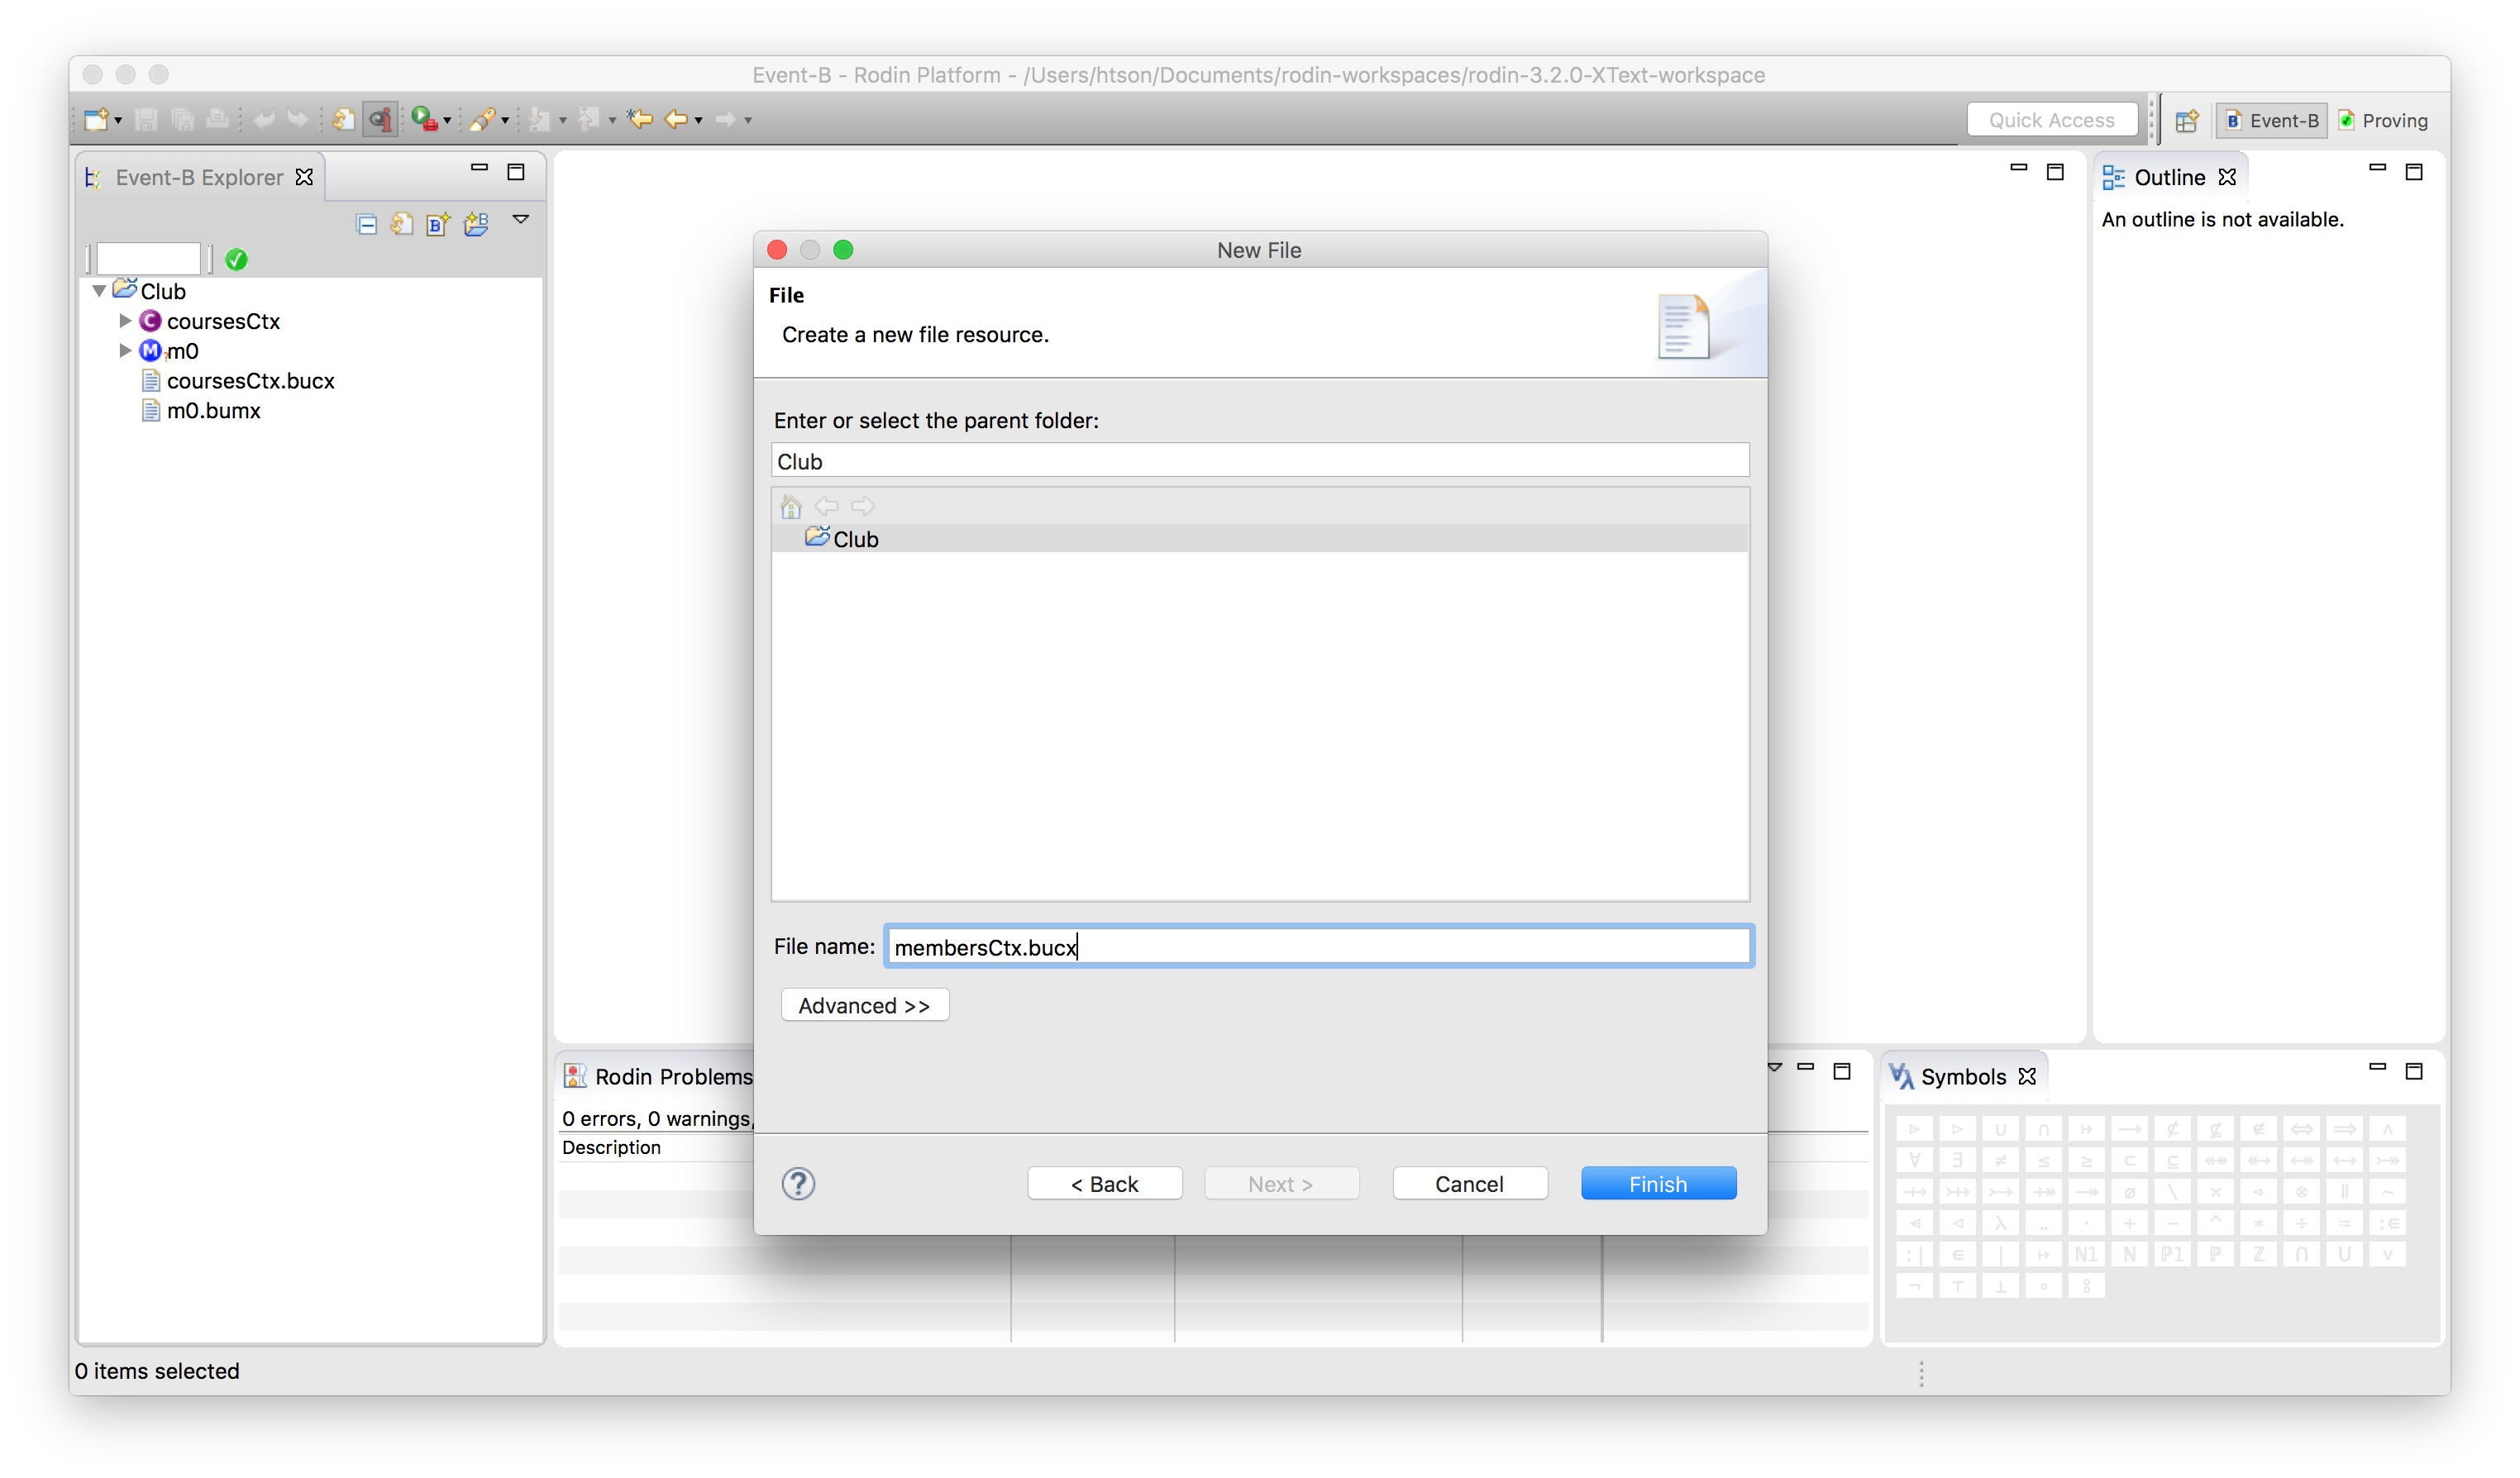
\includegraphics[width=0.9\textwidth]{figures/CreateMembersCtx}
    \fi
    \caption{Create membersCtx.bucx}
    \label{fig:CreateMembersCtx}
  \end{figure}

\item[Step 2. Set the content of membersCtx.bucx] \textbf{Set the content of ``membersCtx.bucx'' as follows}.
  \begin{center}
    \begin{Bcode}
      \ifplastex
      \Bcontext{} memebersCtx\\
      \Bsets{} MEM\\
      \Baxioms\\
      @axm0_1: "finite(MEM)"\\
      \Bend
      \else
      \Bcontext{} memebersCtx\\
      \Bsets{} MEM\\
      \Baxioms\\
      \Btab @axm0_1: "\(\finite(MEM)\)"\\
      \Bend
      \fi
    \end{Bcode}
  \end{center}

\item [Step 3. Auto-format the code] \textbf{Automatically format the content of ``membersCtx.bucx''} by using short-cut (e.g., on Mac OS: Cmd+Shift+F).

\item[Step 4. Save the file] <b>Save the file \textbf{``membersCtx.bucx''}.
\end{description}

\textbf{Conclusion} By now, the XContext ``membersCtx.bucx'' and the corresponding Rodin Context ``membersCtx'' should be visible in the Event-B Explorer (see Figure~\ref{fig:membersCtx}.
  \begin{figure}[!htbp]
    \centering
    \ifplastex
    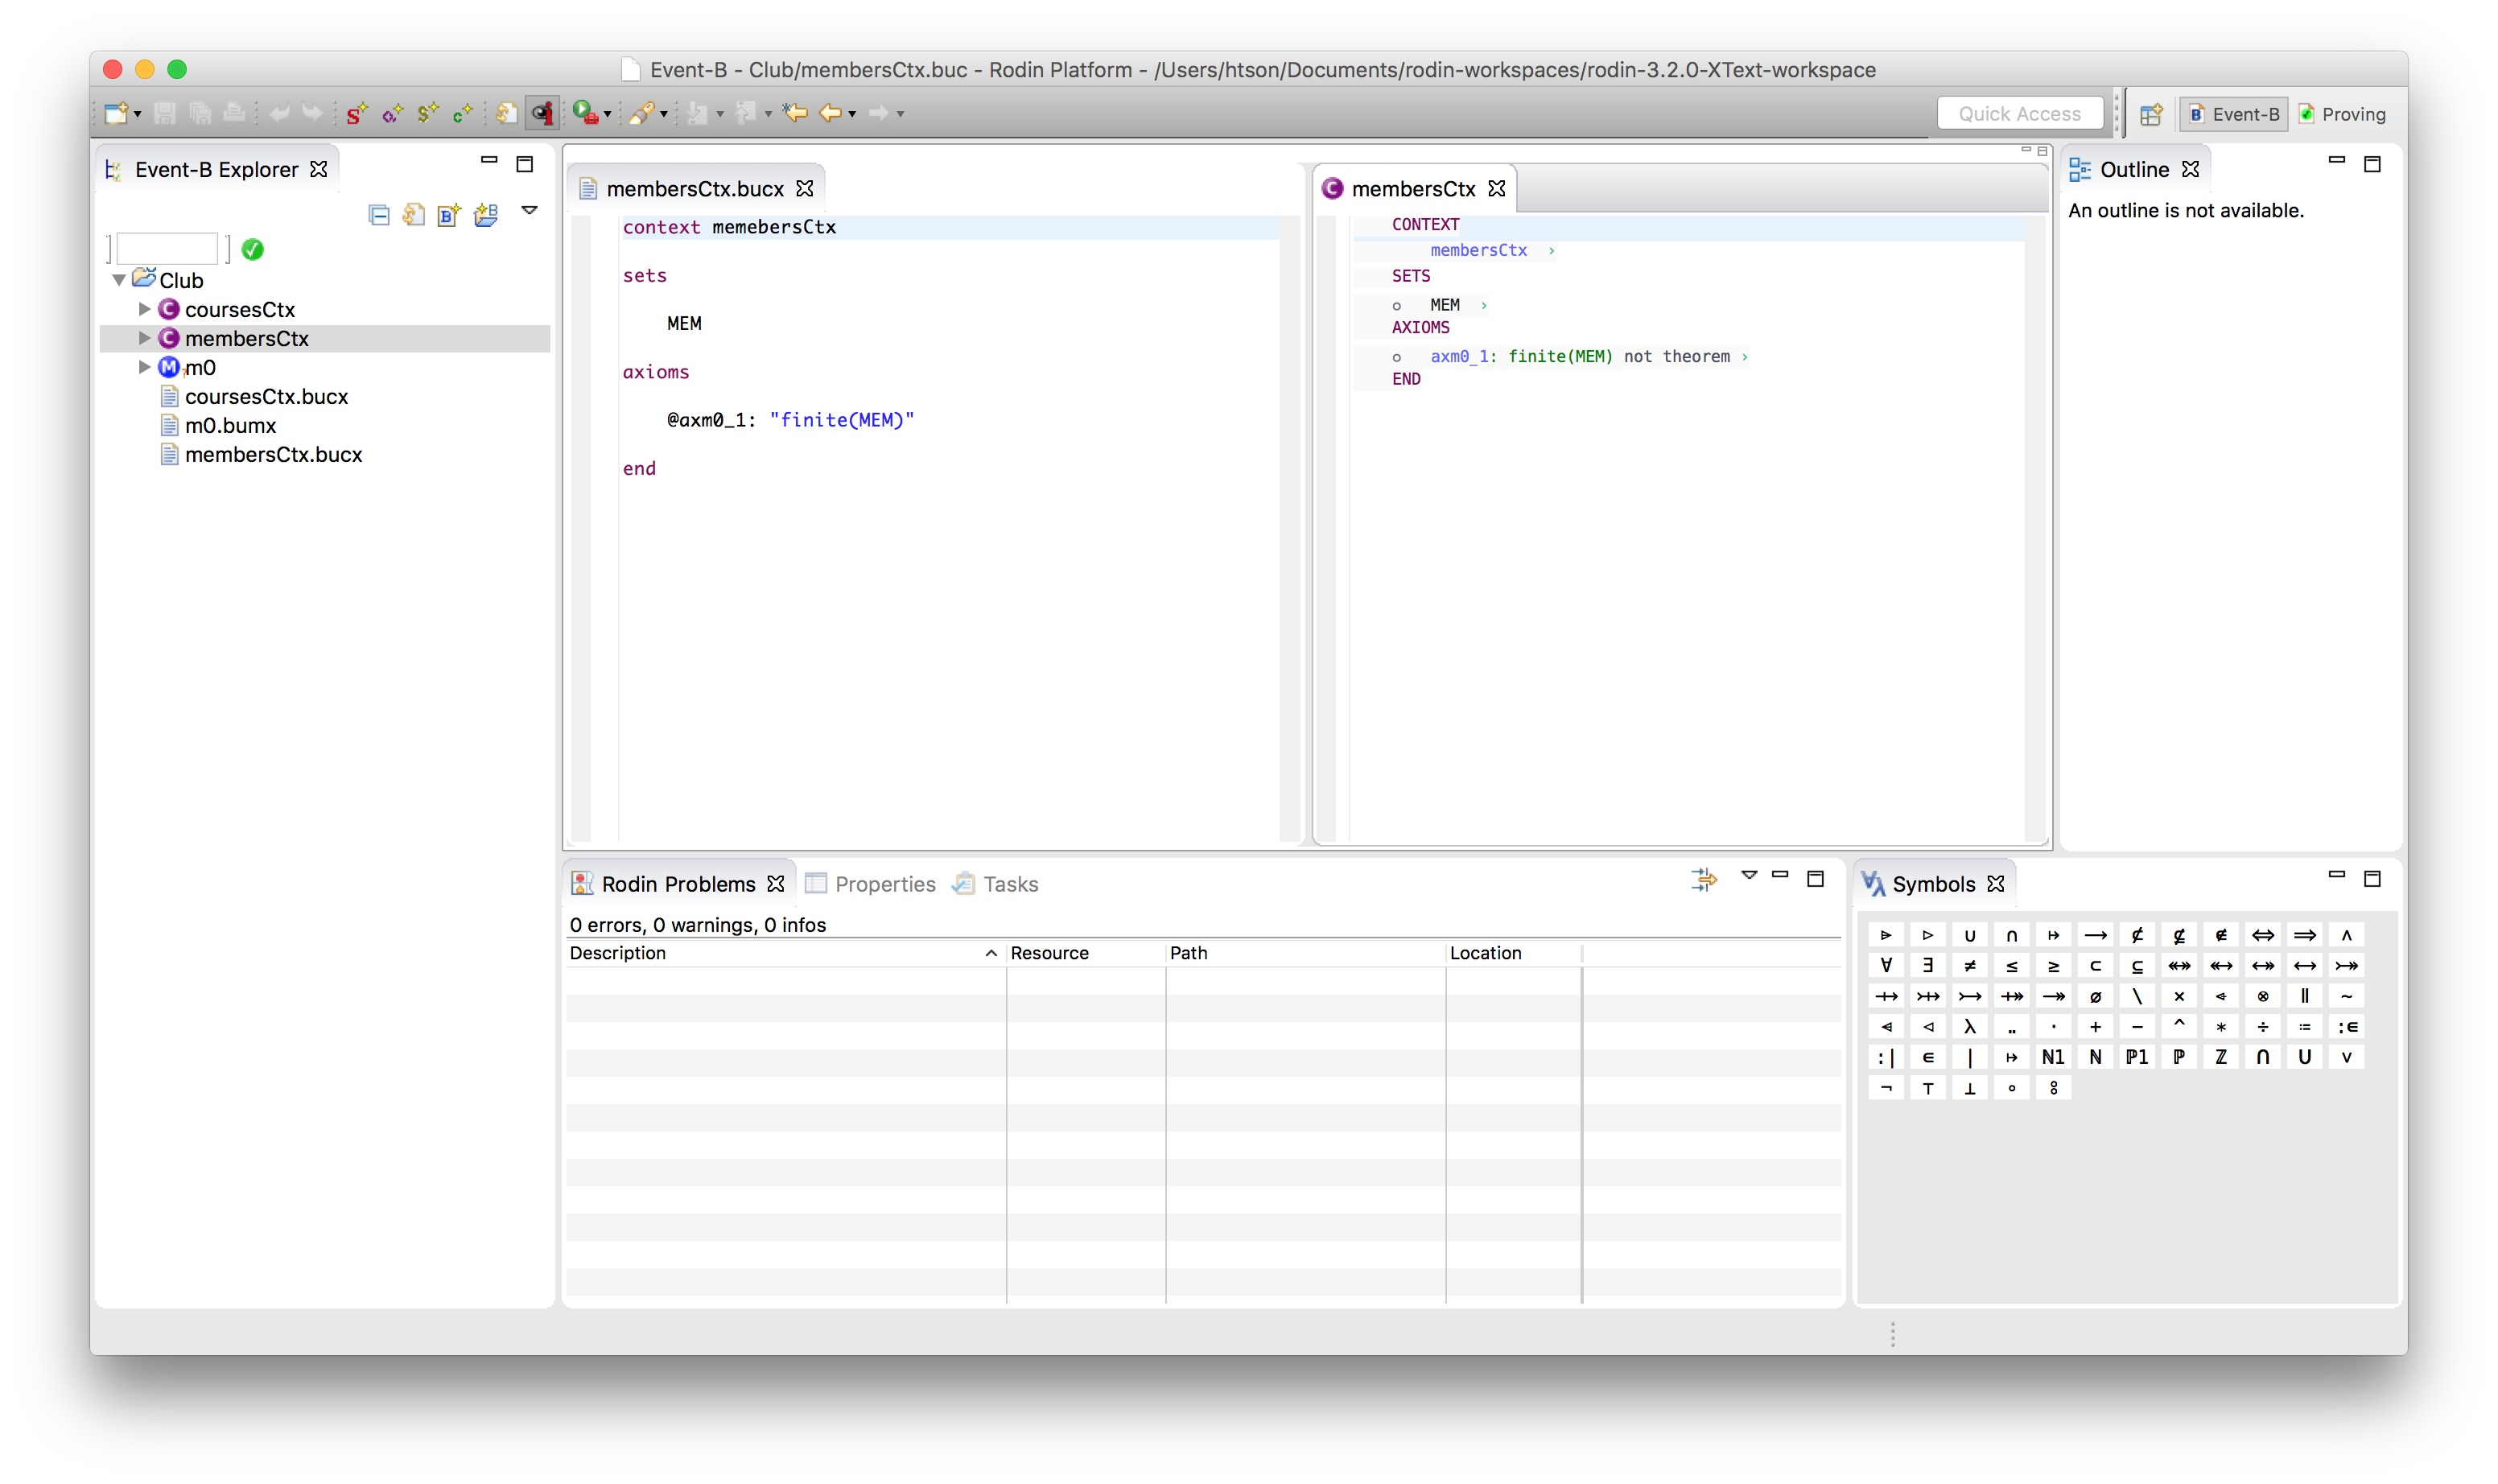
\includegraphics[width=512]{figures/MembersCtx}
    \else
    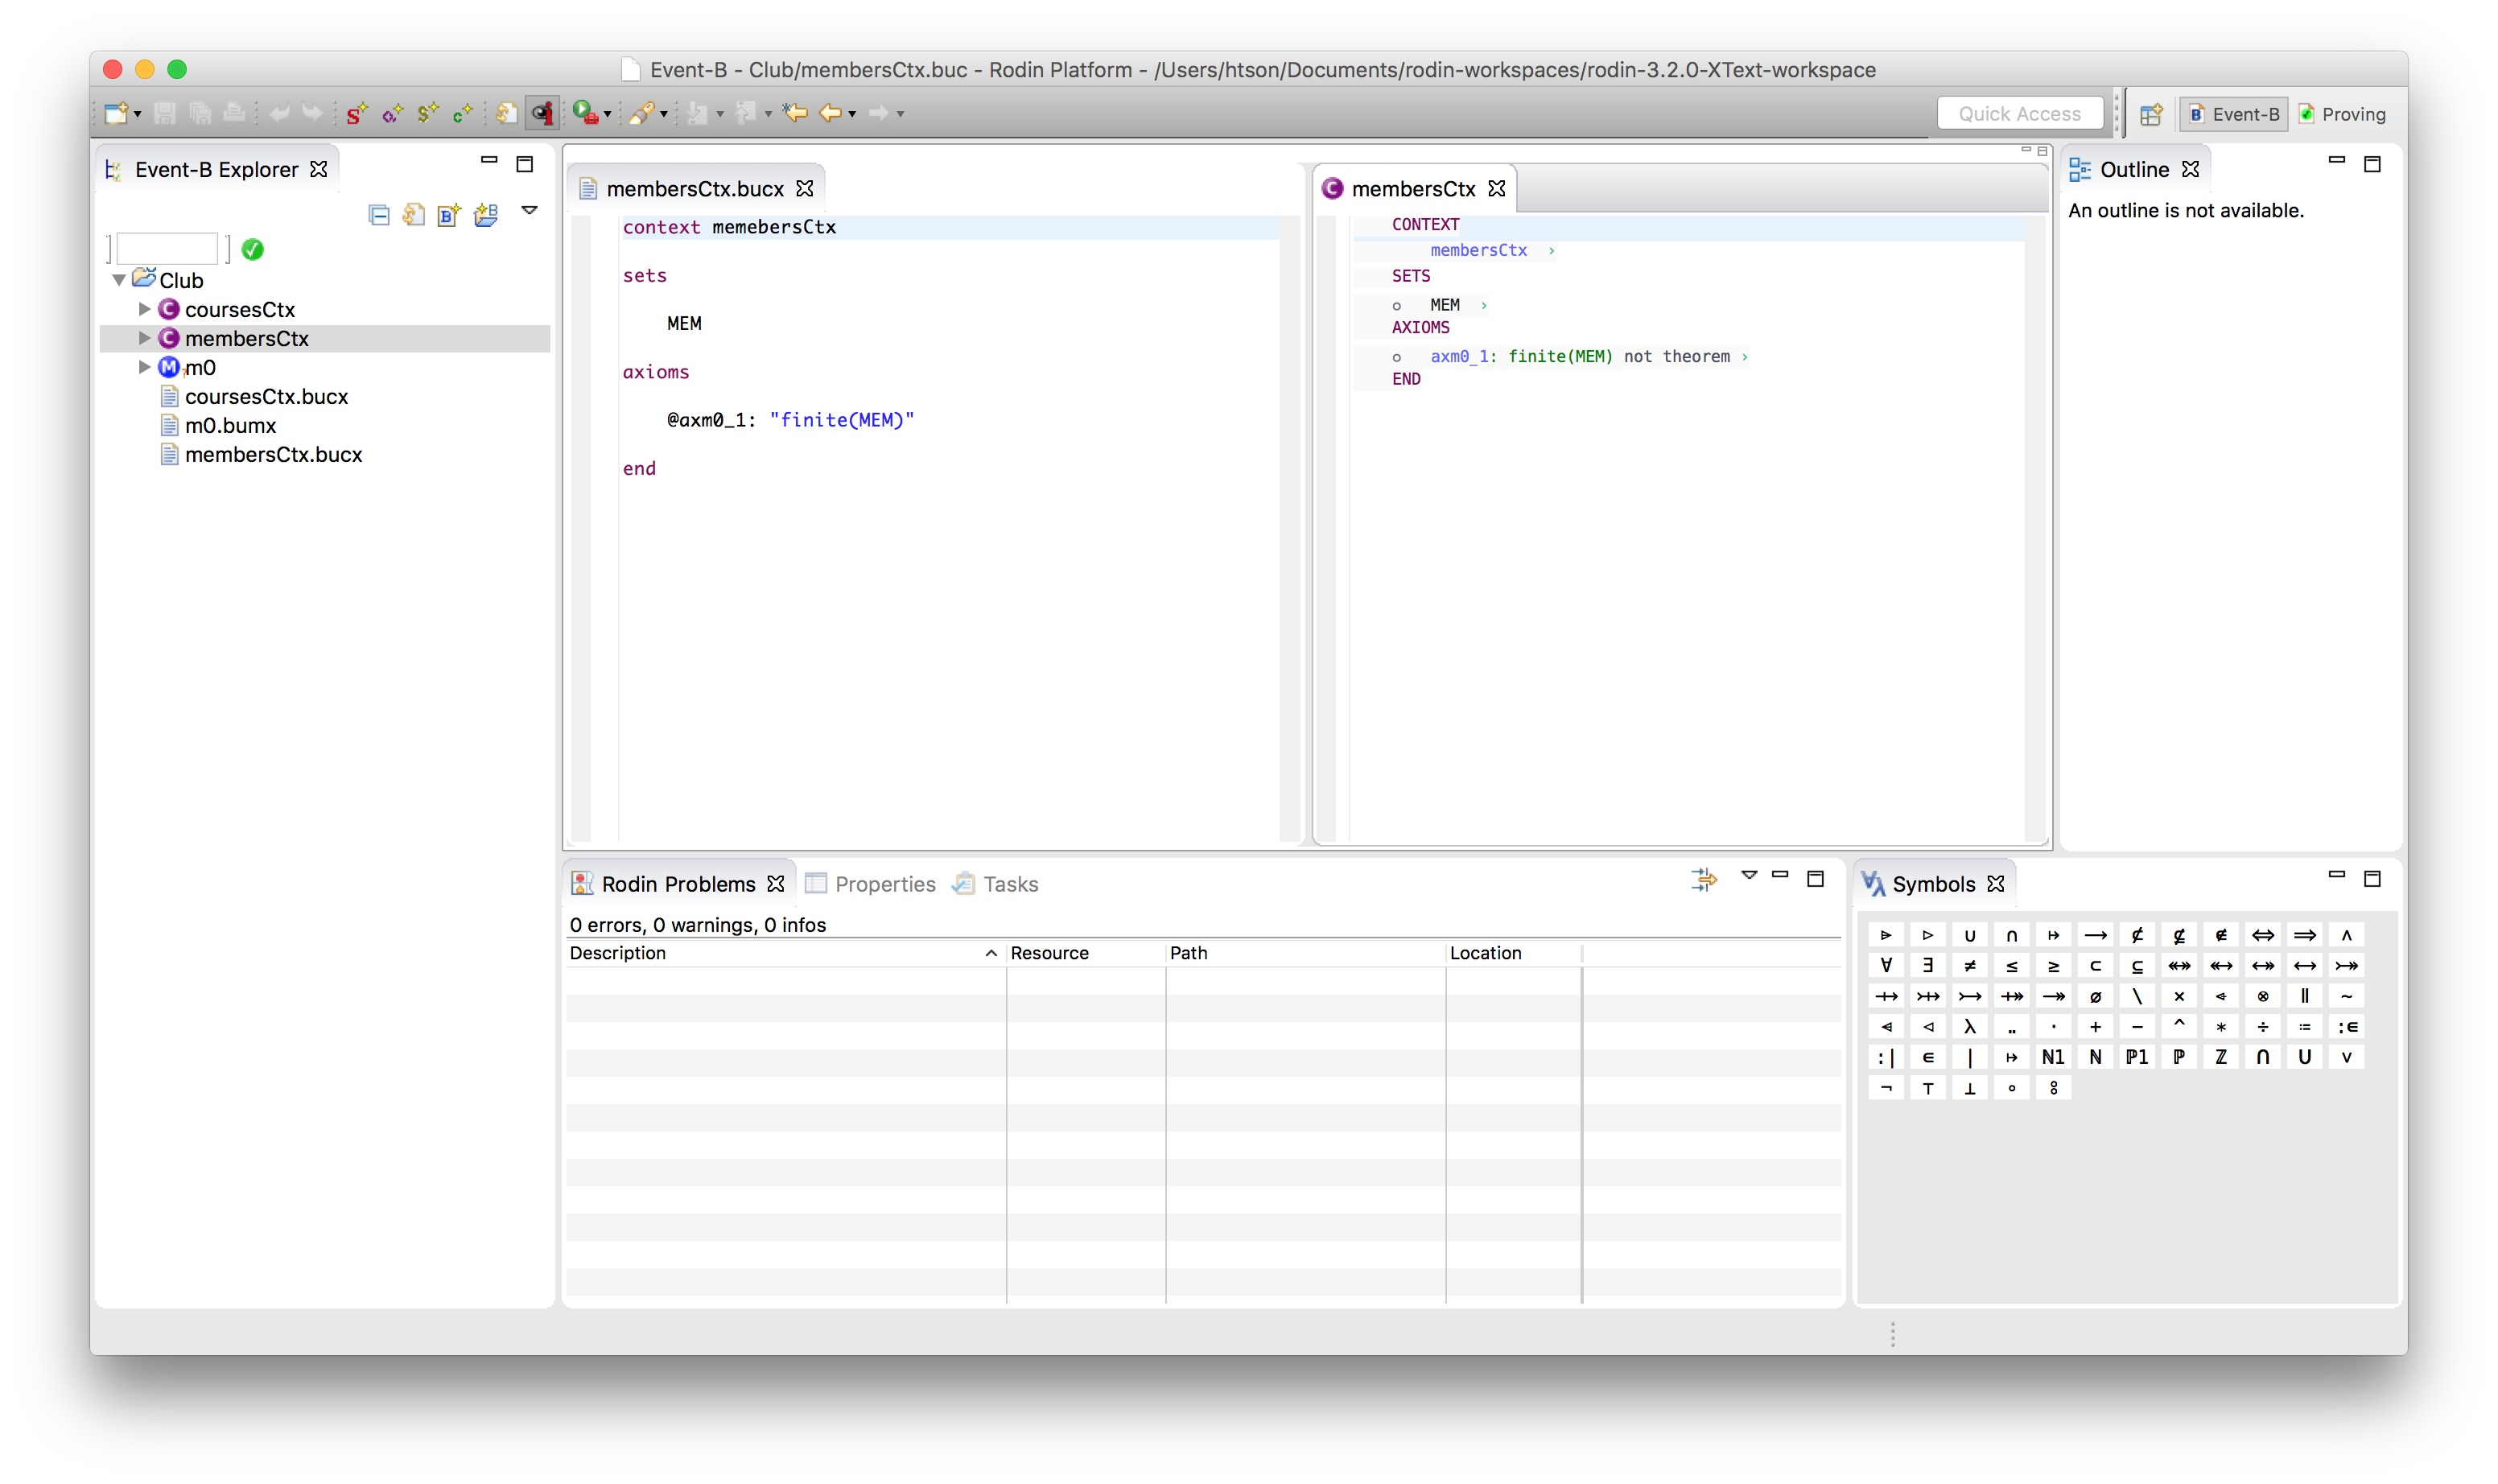
\includegraphics[width=0.9\textwidth]{figures/MembersCtx}
    \fi
    \caption{XContext membersCtx.bucx}
    \label{fig:membersCtx}
  \end{figure}
\paragraph{Task 5.2. Create an extended XContext participantsCtx.bucx}
\textbf{Introduction} The purpose of this sub-task is to create an extended XContext ``participantsCtx.bucx'' within the ``Club'' project.

\begin{description}
\item[Step 1. Create a new XContext participantsCtx.bucx] \textbf{Create a new XContext} named ``participantsCtx.bucx'' using the \emph{New File wizard} (see Figure~\ref{fig:CreateParticipantsCtx}.
  \begin{figure}[!htbp]
    \centering
    \ifplastex
    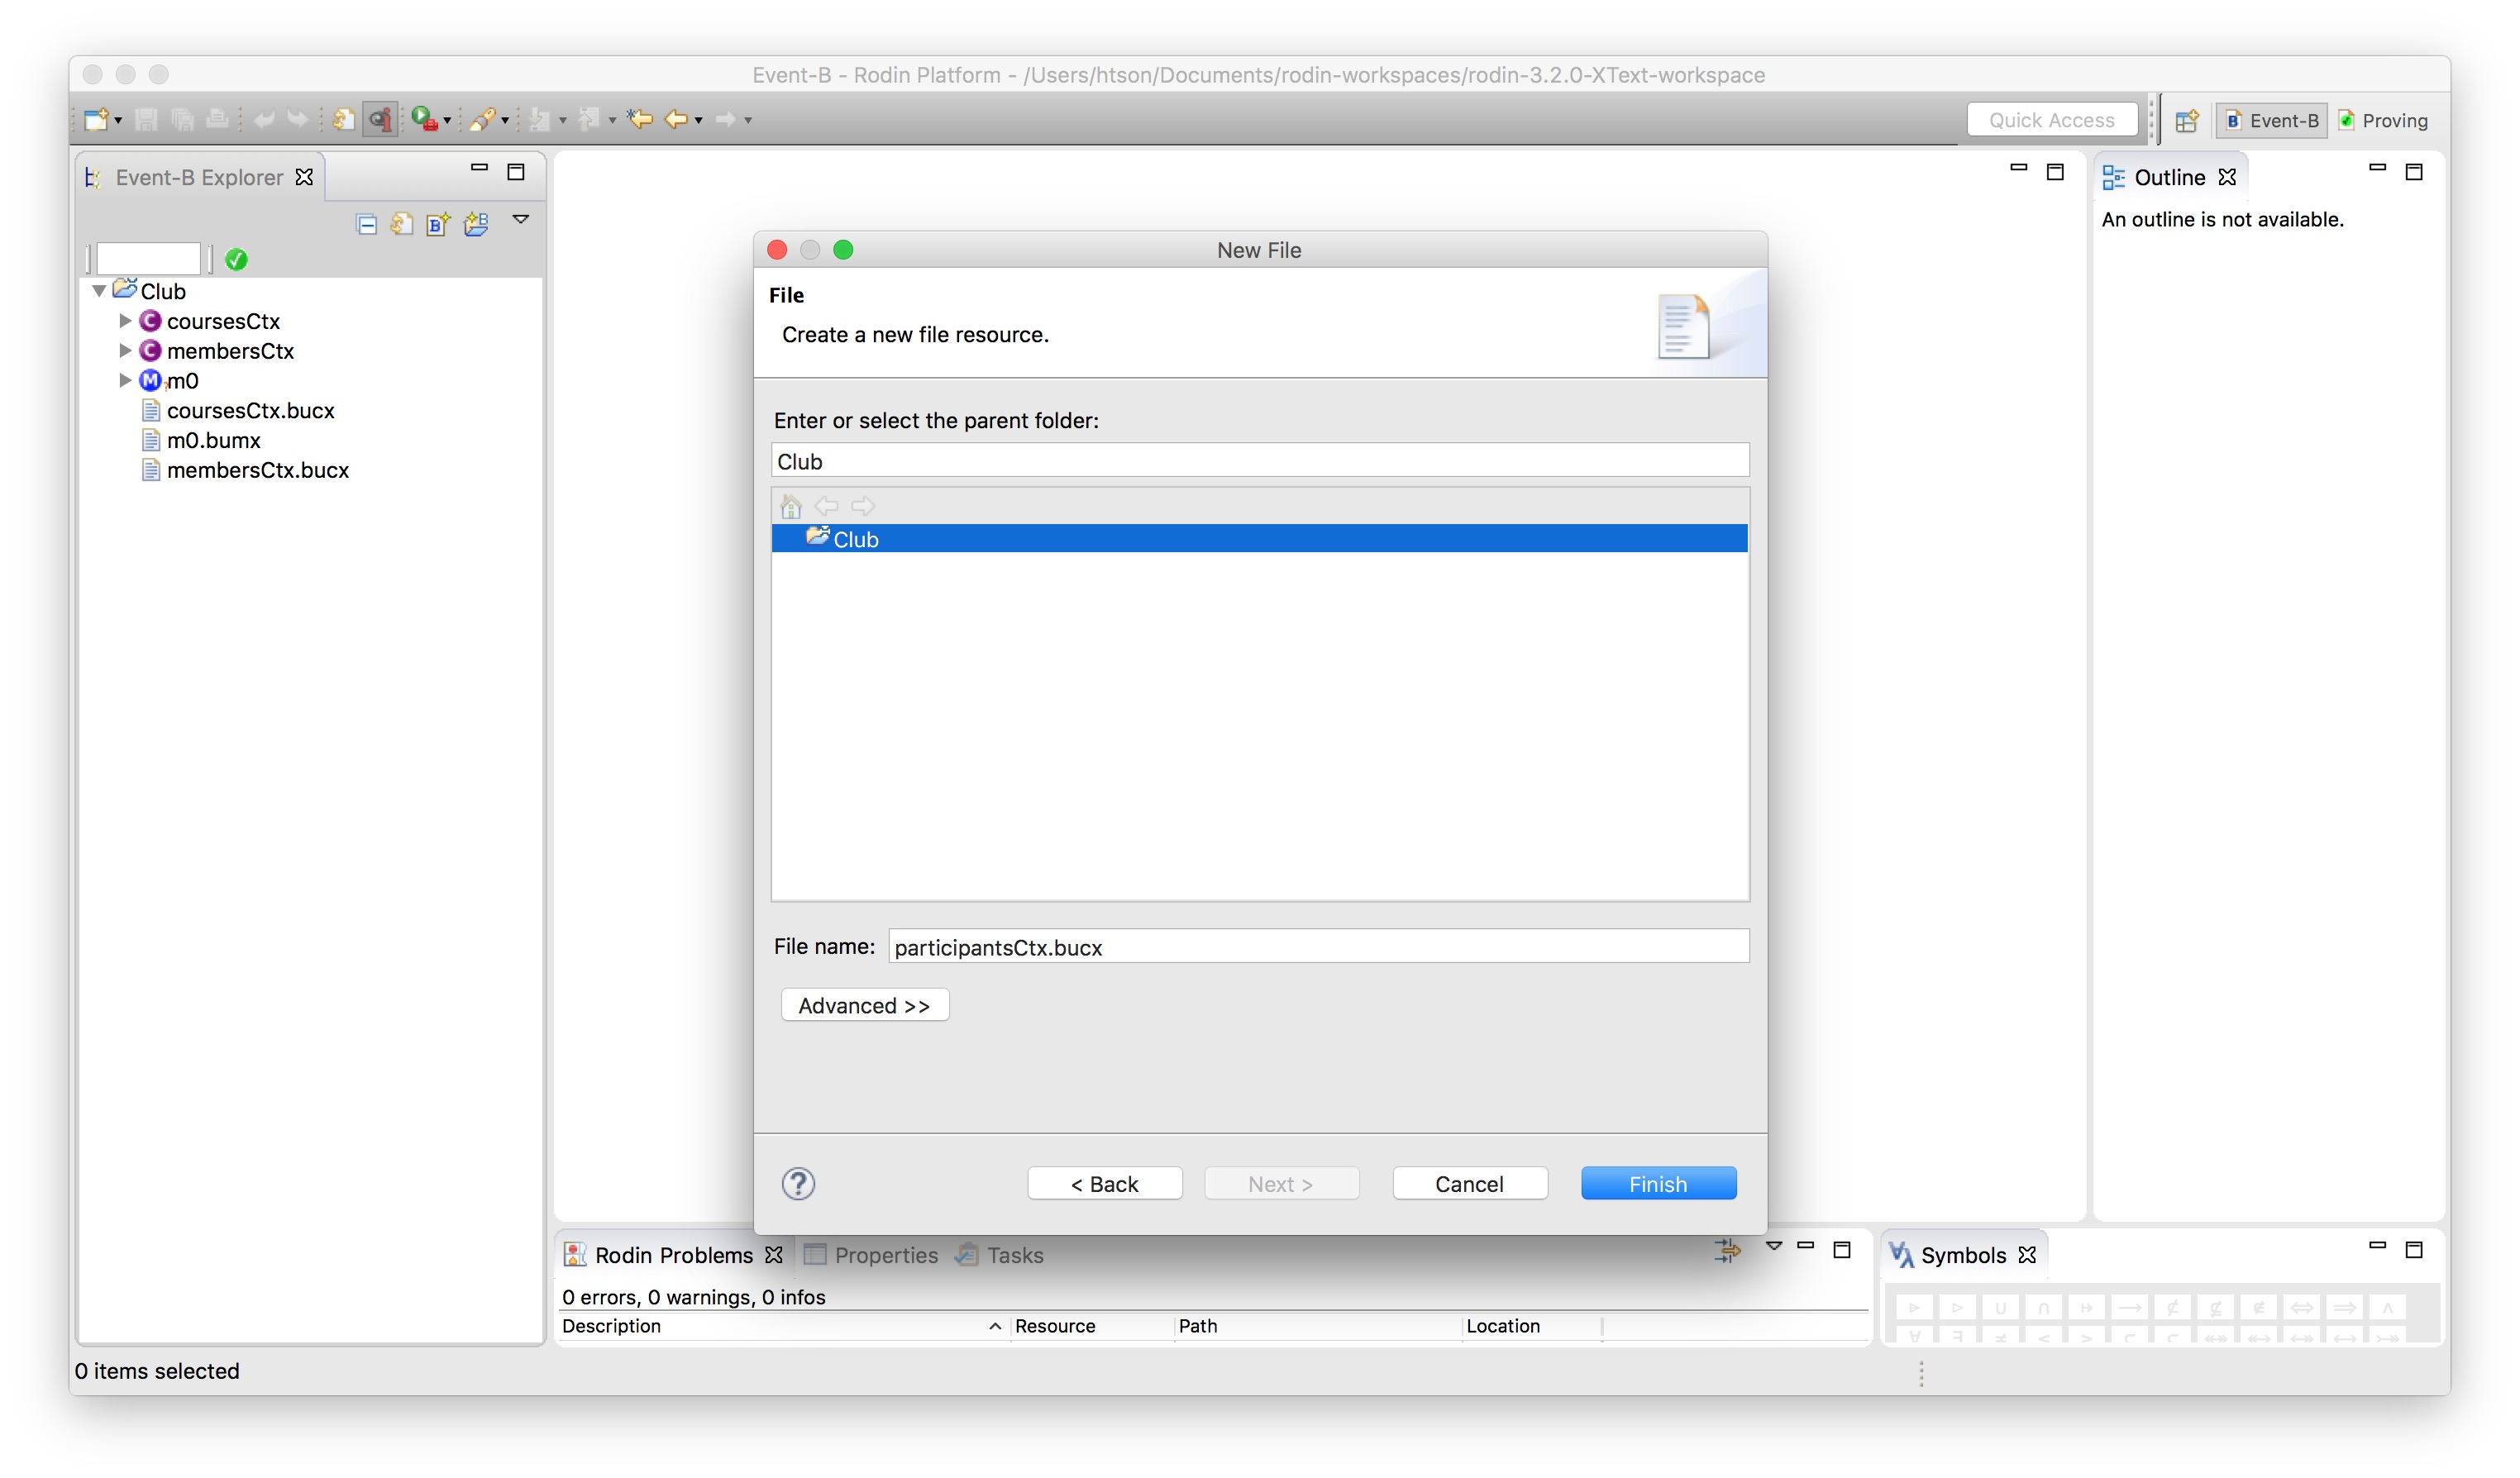
\includegraphics[width=512]{figures/CreateParticipantsCtx}
    \else
    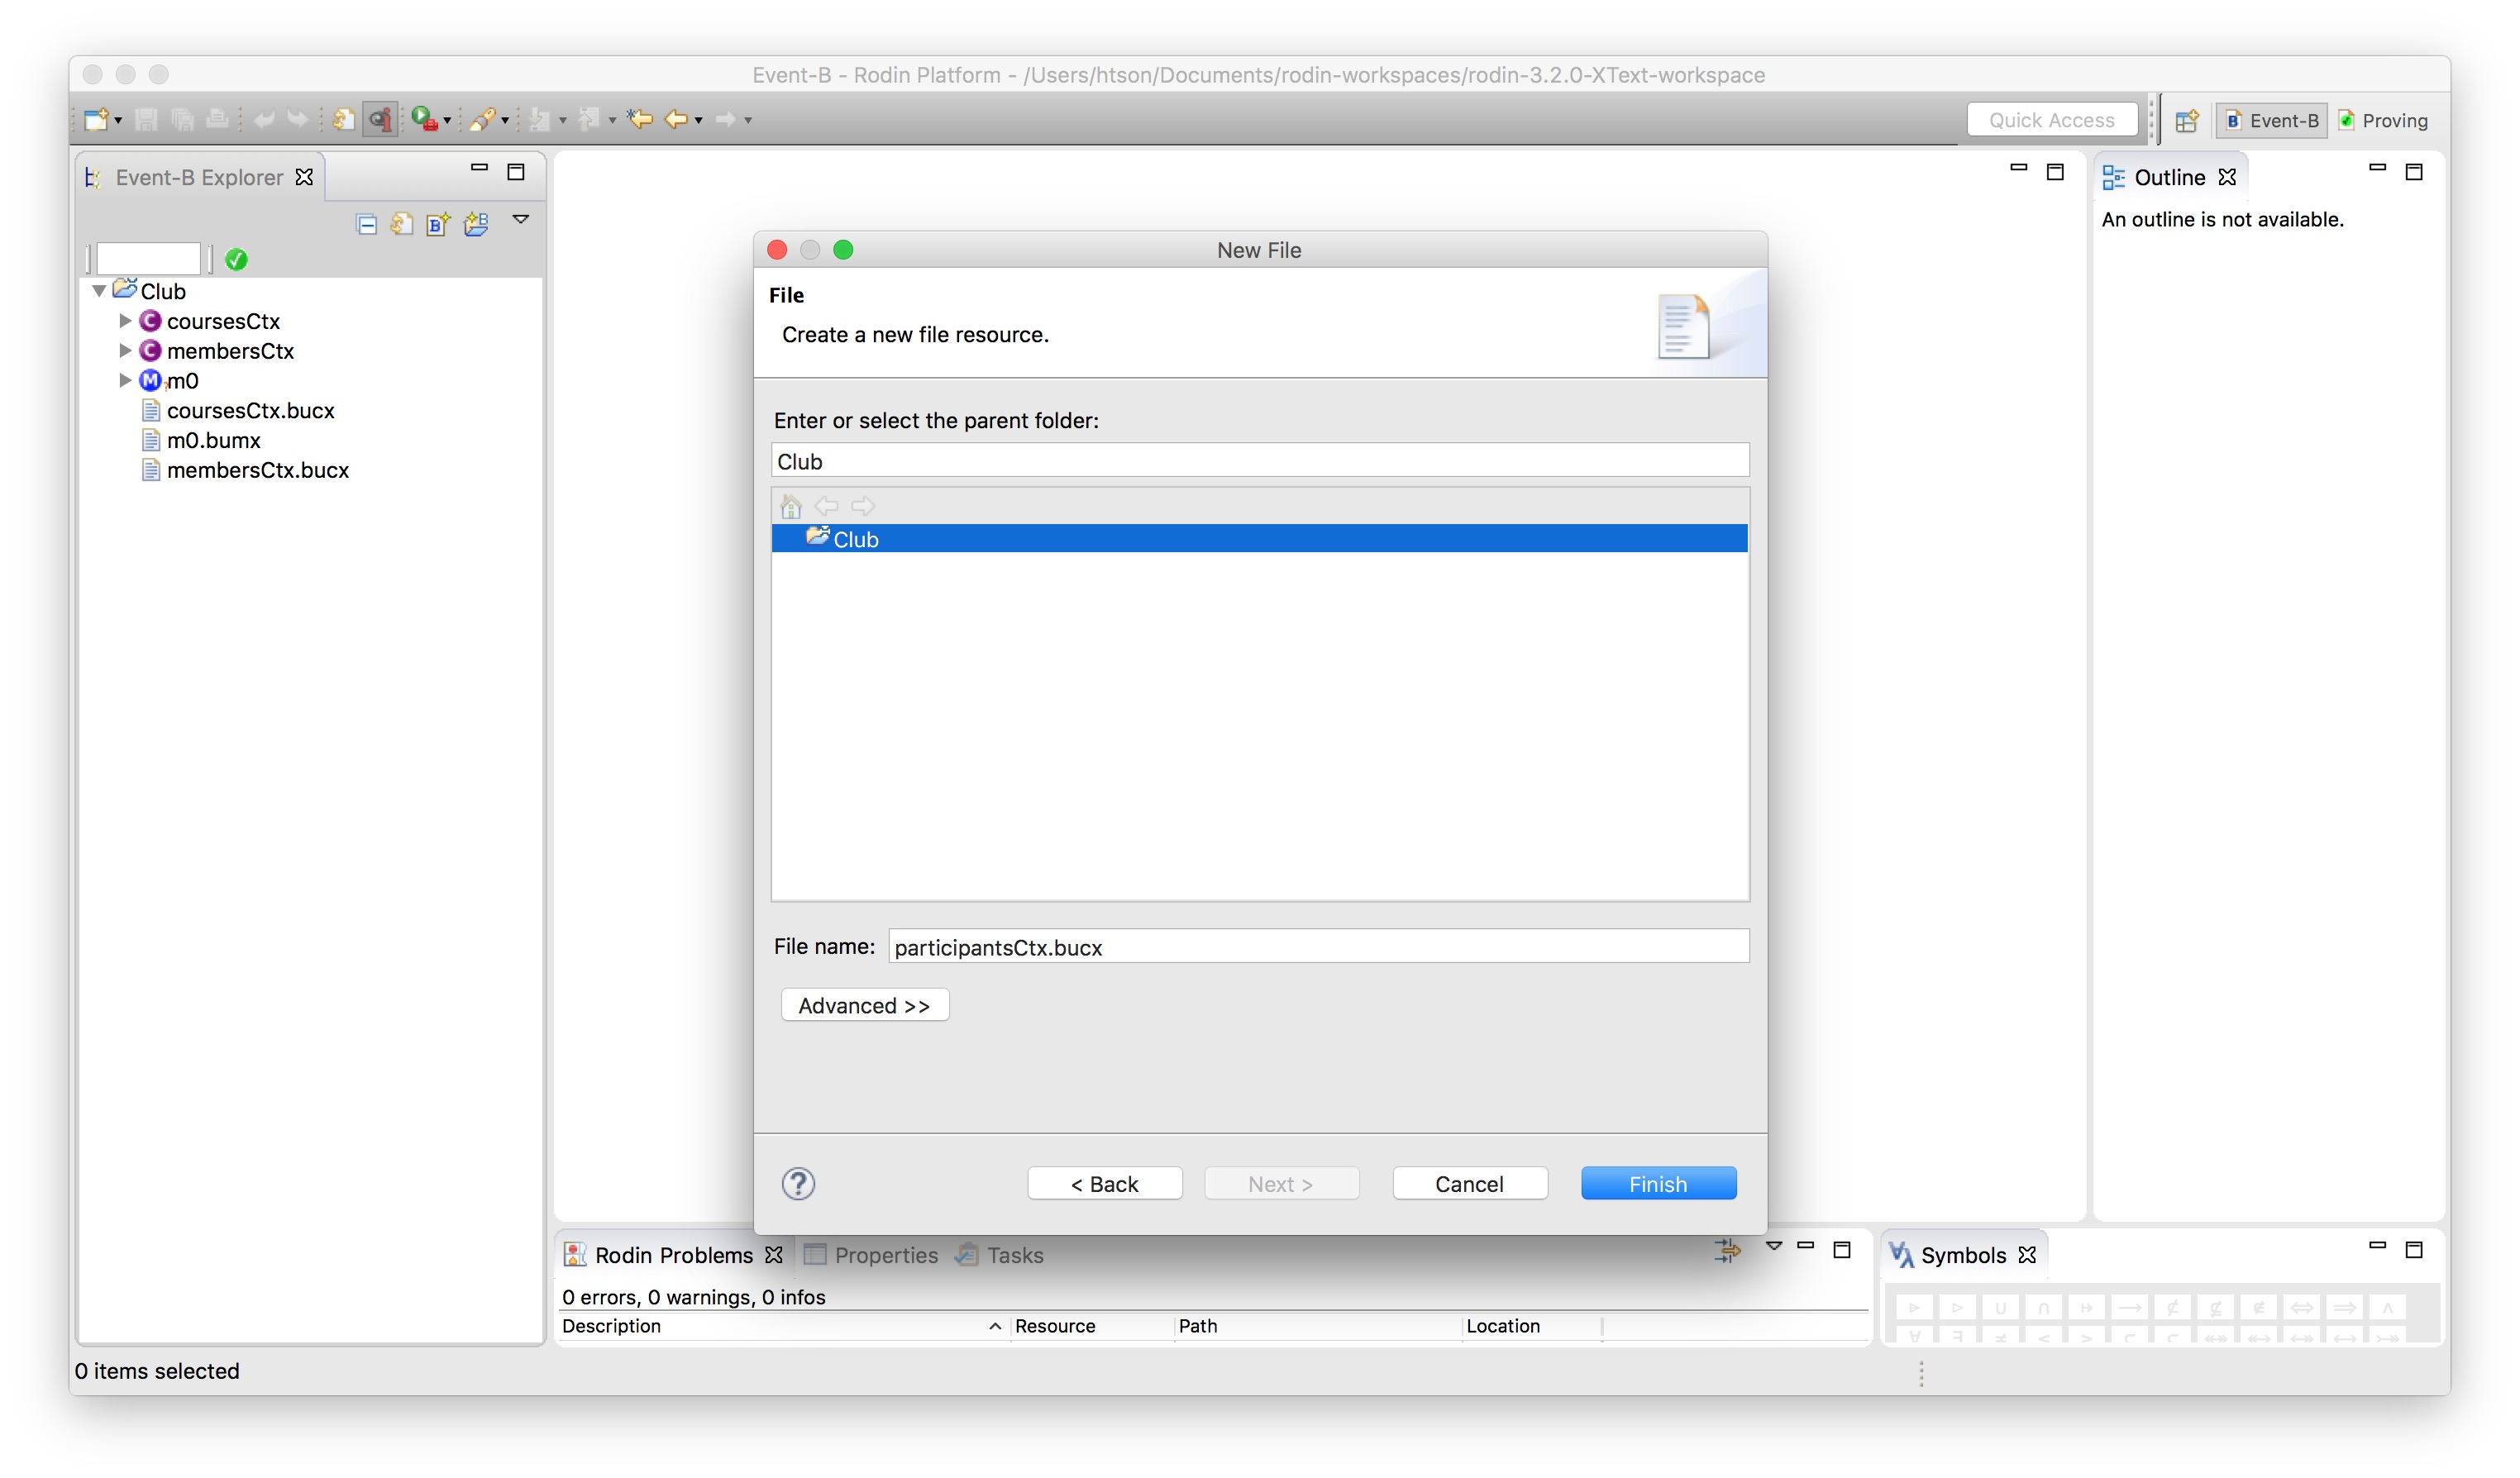
\includegraphics[width=0.9\textwidth]{figures/CreateParticipantsCtx}
    \fi
    \caption{Create participantsCtx.bucx}
    \label{fig:CreateParticipantsCtx}
  \end{figure}

\item[Step 2. Set the content of participantsCtx.bucx] \textbf{Set the content of ``participantsCtx.bucx'' as follows}.
  \begin{center}
    \begin{Bcode}
      \ifplastex
      \Bcontext{} participantsCtx\\
      \Bextends{} membersCtx\\
      \Bconstants{} PRTCPT\\
      \Baxioms\\
      @axm1_2: "PRTCPT ∈ ℙ(MEM)"\\
      @thm1_1: "finite(PRTCPT)" \Btheorem\\
      \Bend
      \else
      \Bcontext{} participantsCtx\\
      \Bextends{} membersCtx\\
      \Bconstants{} PRTCPT\\
      \Baxioms\\
      \Btab @axm1_2: "\(PRTCPT \in \pow(MEM)\)"\\
      \Btab @thm1_1: "\(\finite(PRTCPT)\)" \Btheorem\\
      \Bend
      \fi
    \end{Bcode}
  \end{center}

\item[Step 3. Auto-format the code] \textbf{Automatically format the content of ``participantsCtx.bucx''} by using short-cut (e.g., on Mac OS: Cmd+Shift+F).

\item[Step 4. Save the file] \textbf{Save the file ``participantsCtx.bucx''}.
\end{description}

\textbf{Conclusion} By now, the XContext ``participantsCtx.bucx'' and the corresponding Rodin Context ``participantsCtx'' should be visible in the Event-B Explorer (see Figure~\ref{fig:ParticipantsCtx}).
  \begin{figure}[!htbp]
    \centering
    \ifplastex
    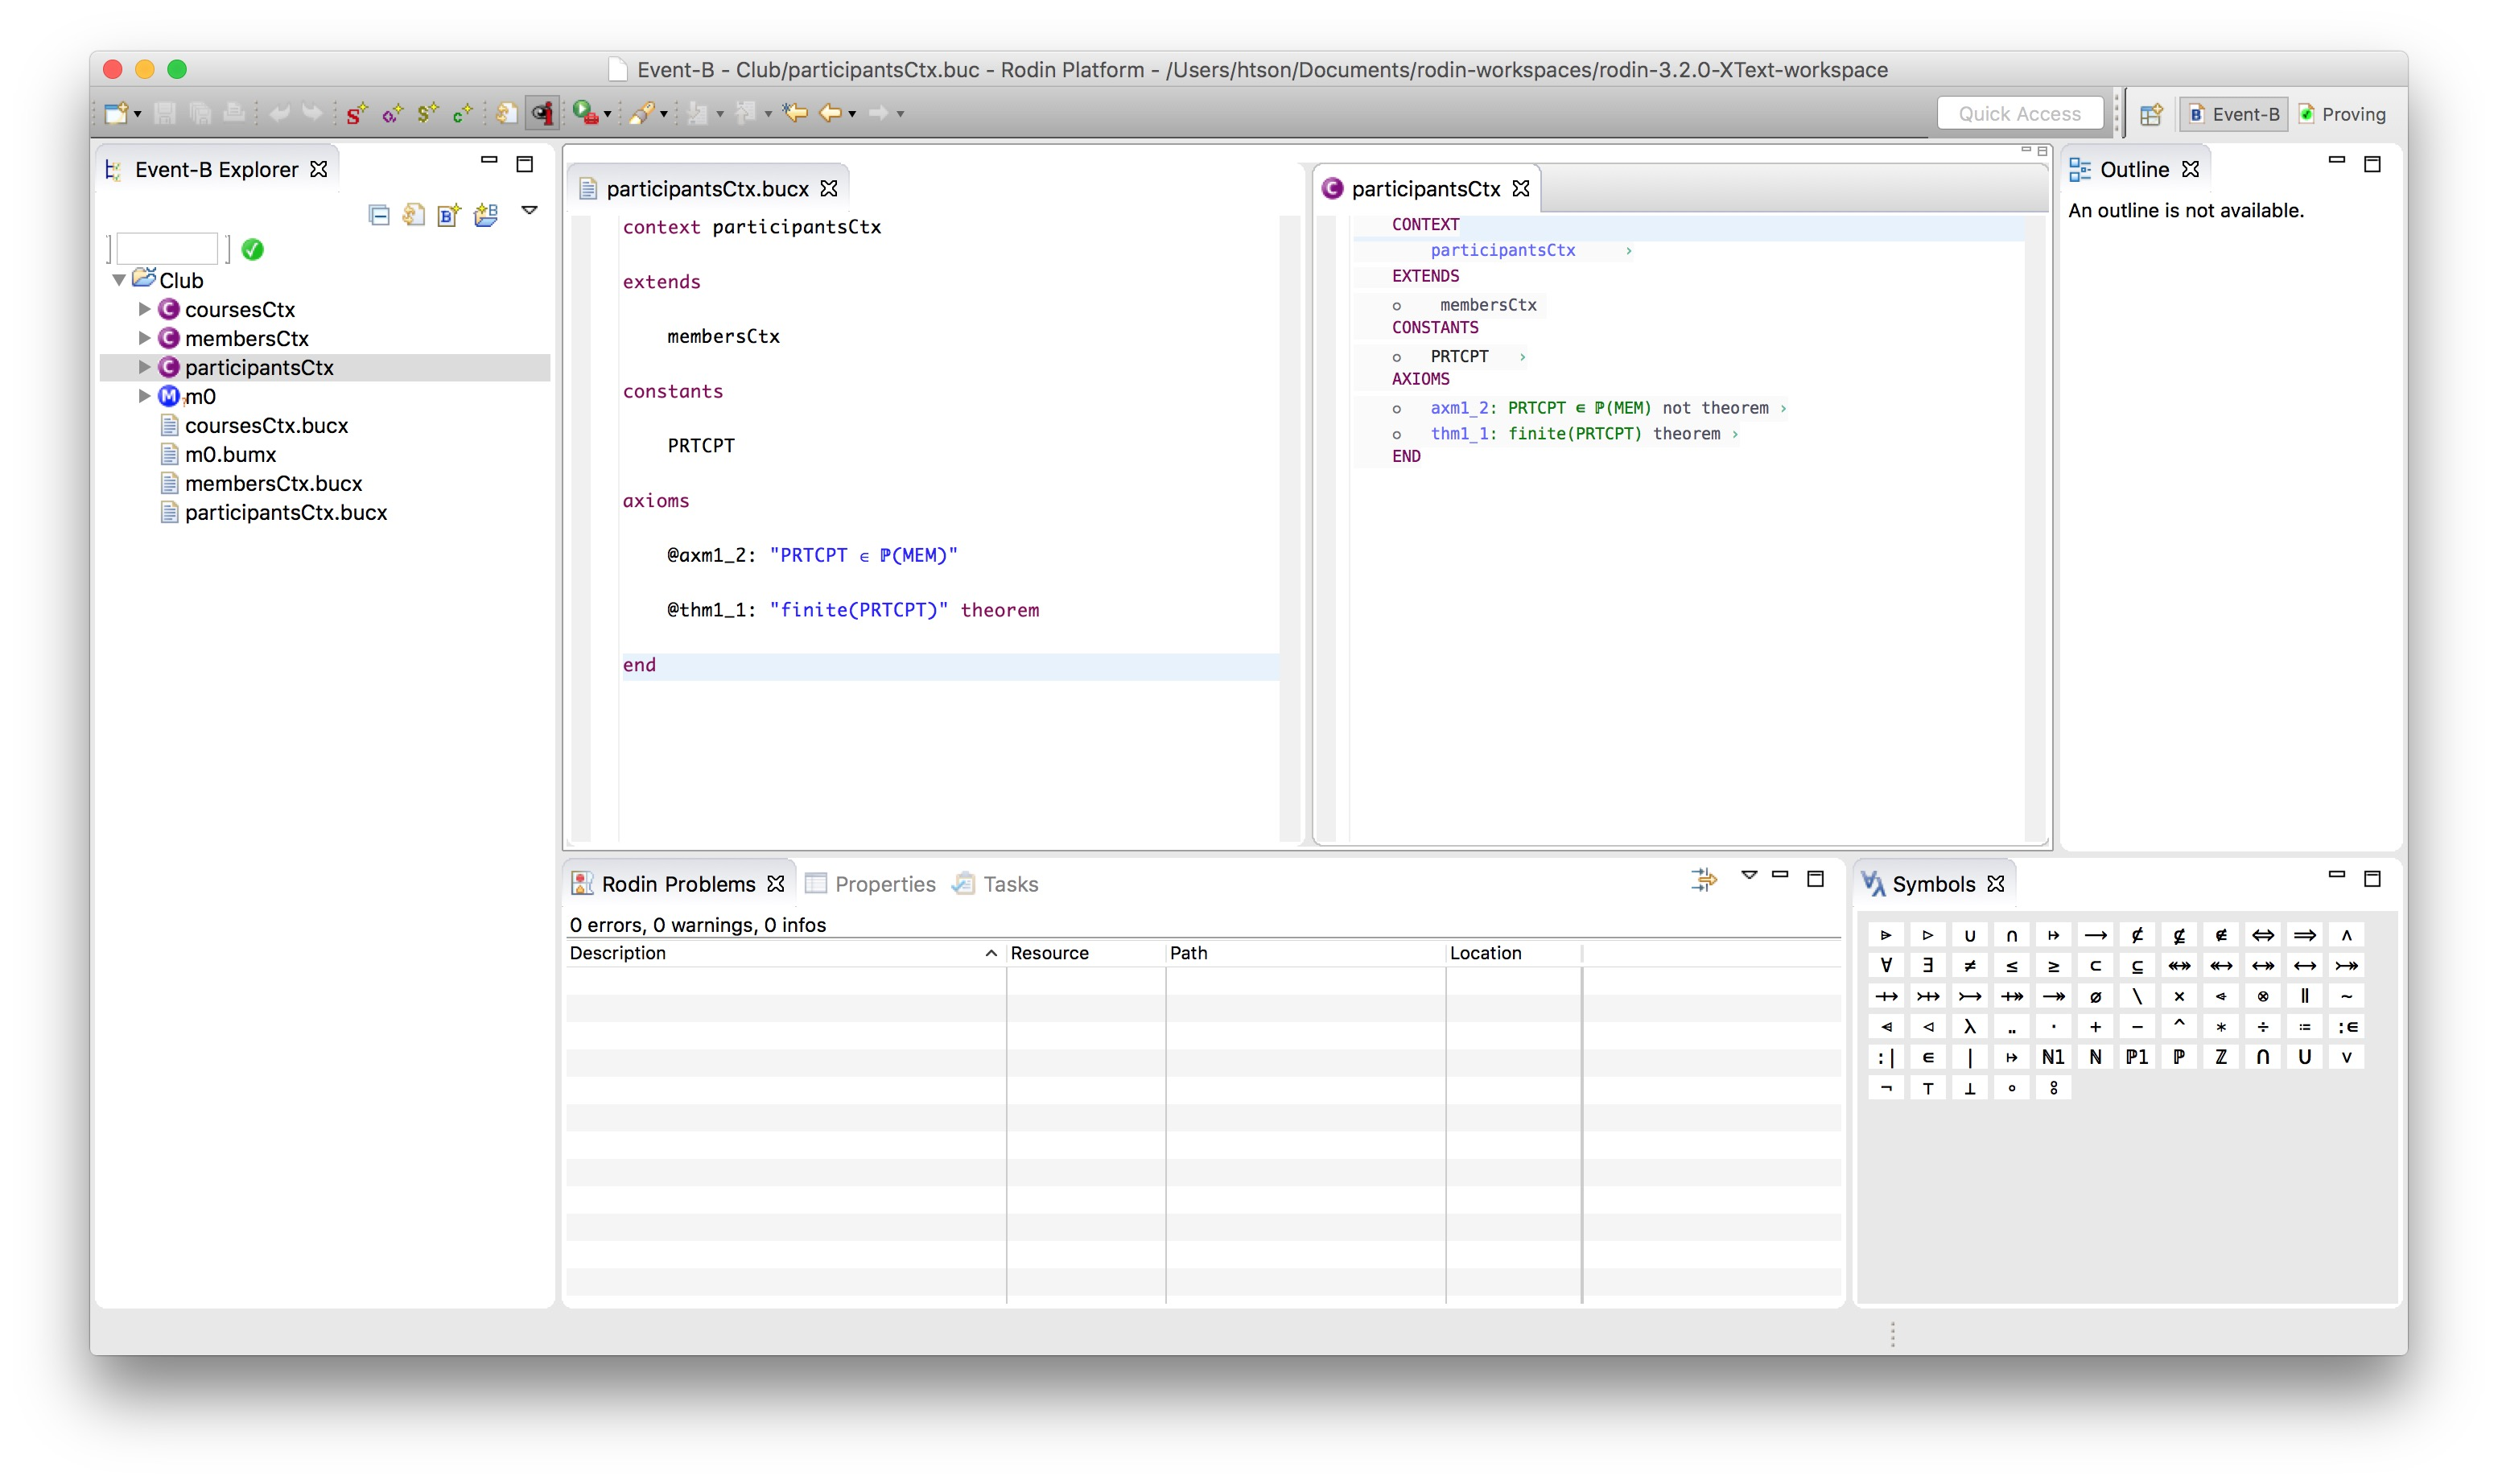
\includegraphics[width=512]{figures/ParticipantsCtx}
    \else
    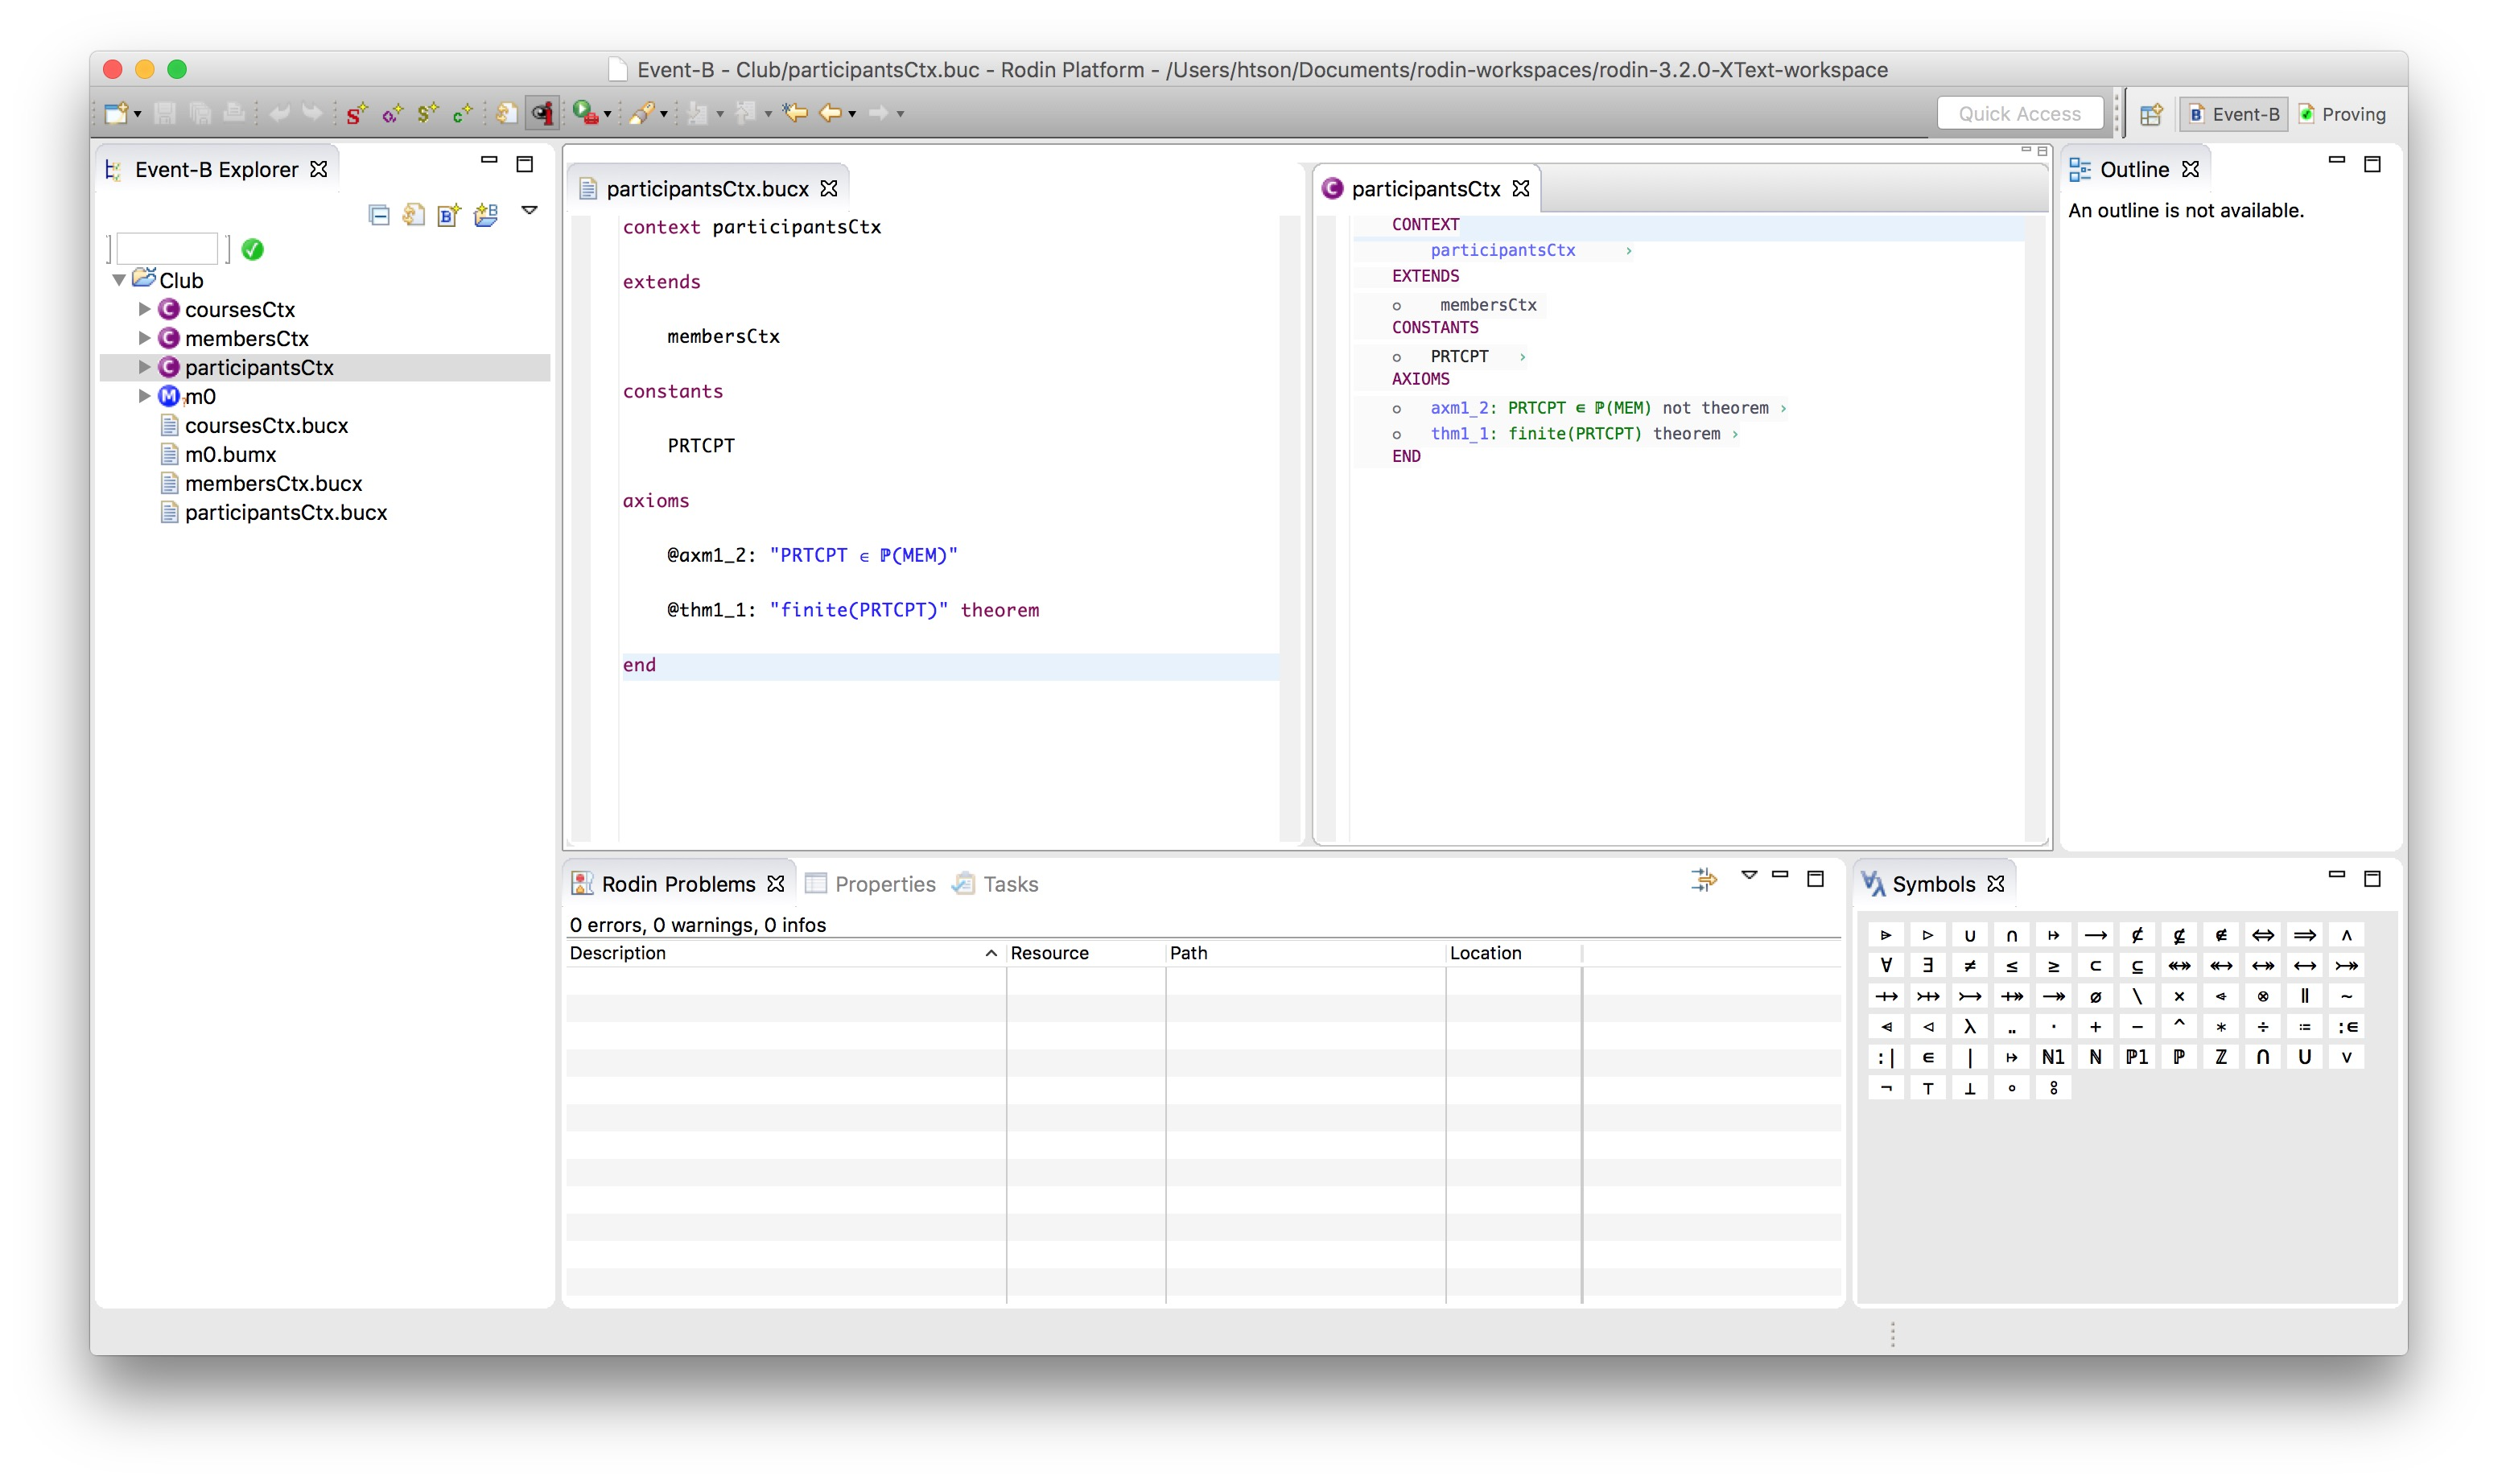
\includegraphics[width=0.9\textwidth]{figures/ParticipantsCtx}
    \fi
    \caption{XContext participantsCtx.bucx}
    \label{fig:ParticipantsCtx}
  \end{figure}

\paragraph{Task 5.3. Create an extended XContext instructorsCtx.bucx}
\textbf{Introduction} The purpose of this sub-task is to create an extended XContext ``instructorsCtx.bucx'' within the ``Club'' project.
\begin{description}
\item[Step 1. Create a new XContext instructorsCtx.bucx] \textbf{Create a new XContext} named ``instructorsCtx.bucx'' using the \emph{New File wizard} (see Figure~\ref{fig:CreateInstructorsCtx}.
  \begin{figure}[!htbp]
    \centering
    \ifplastex
    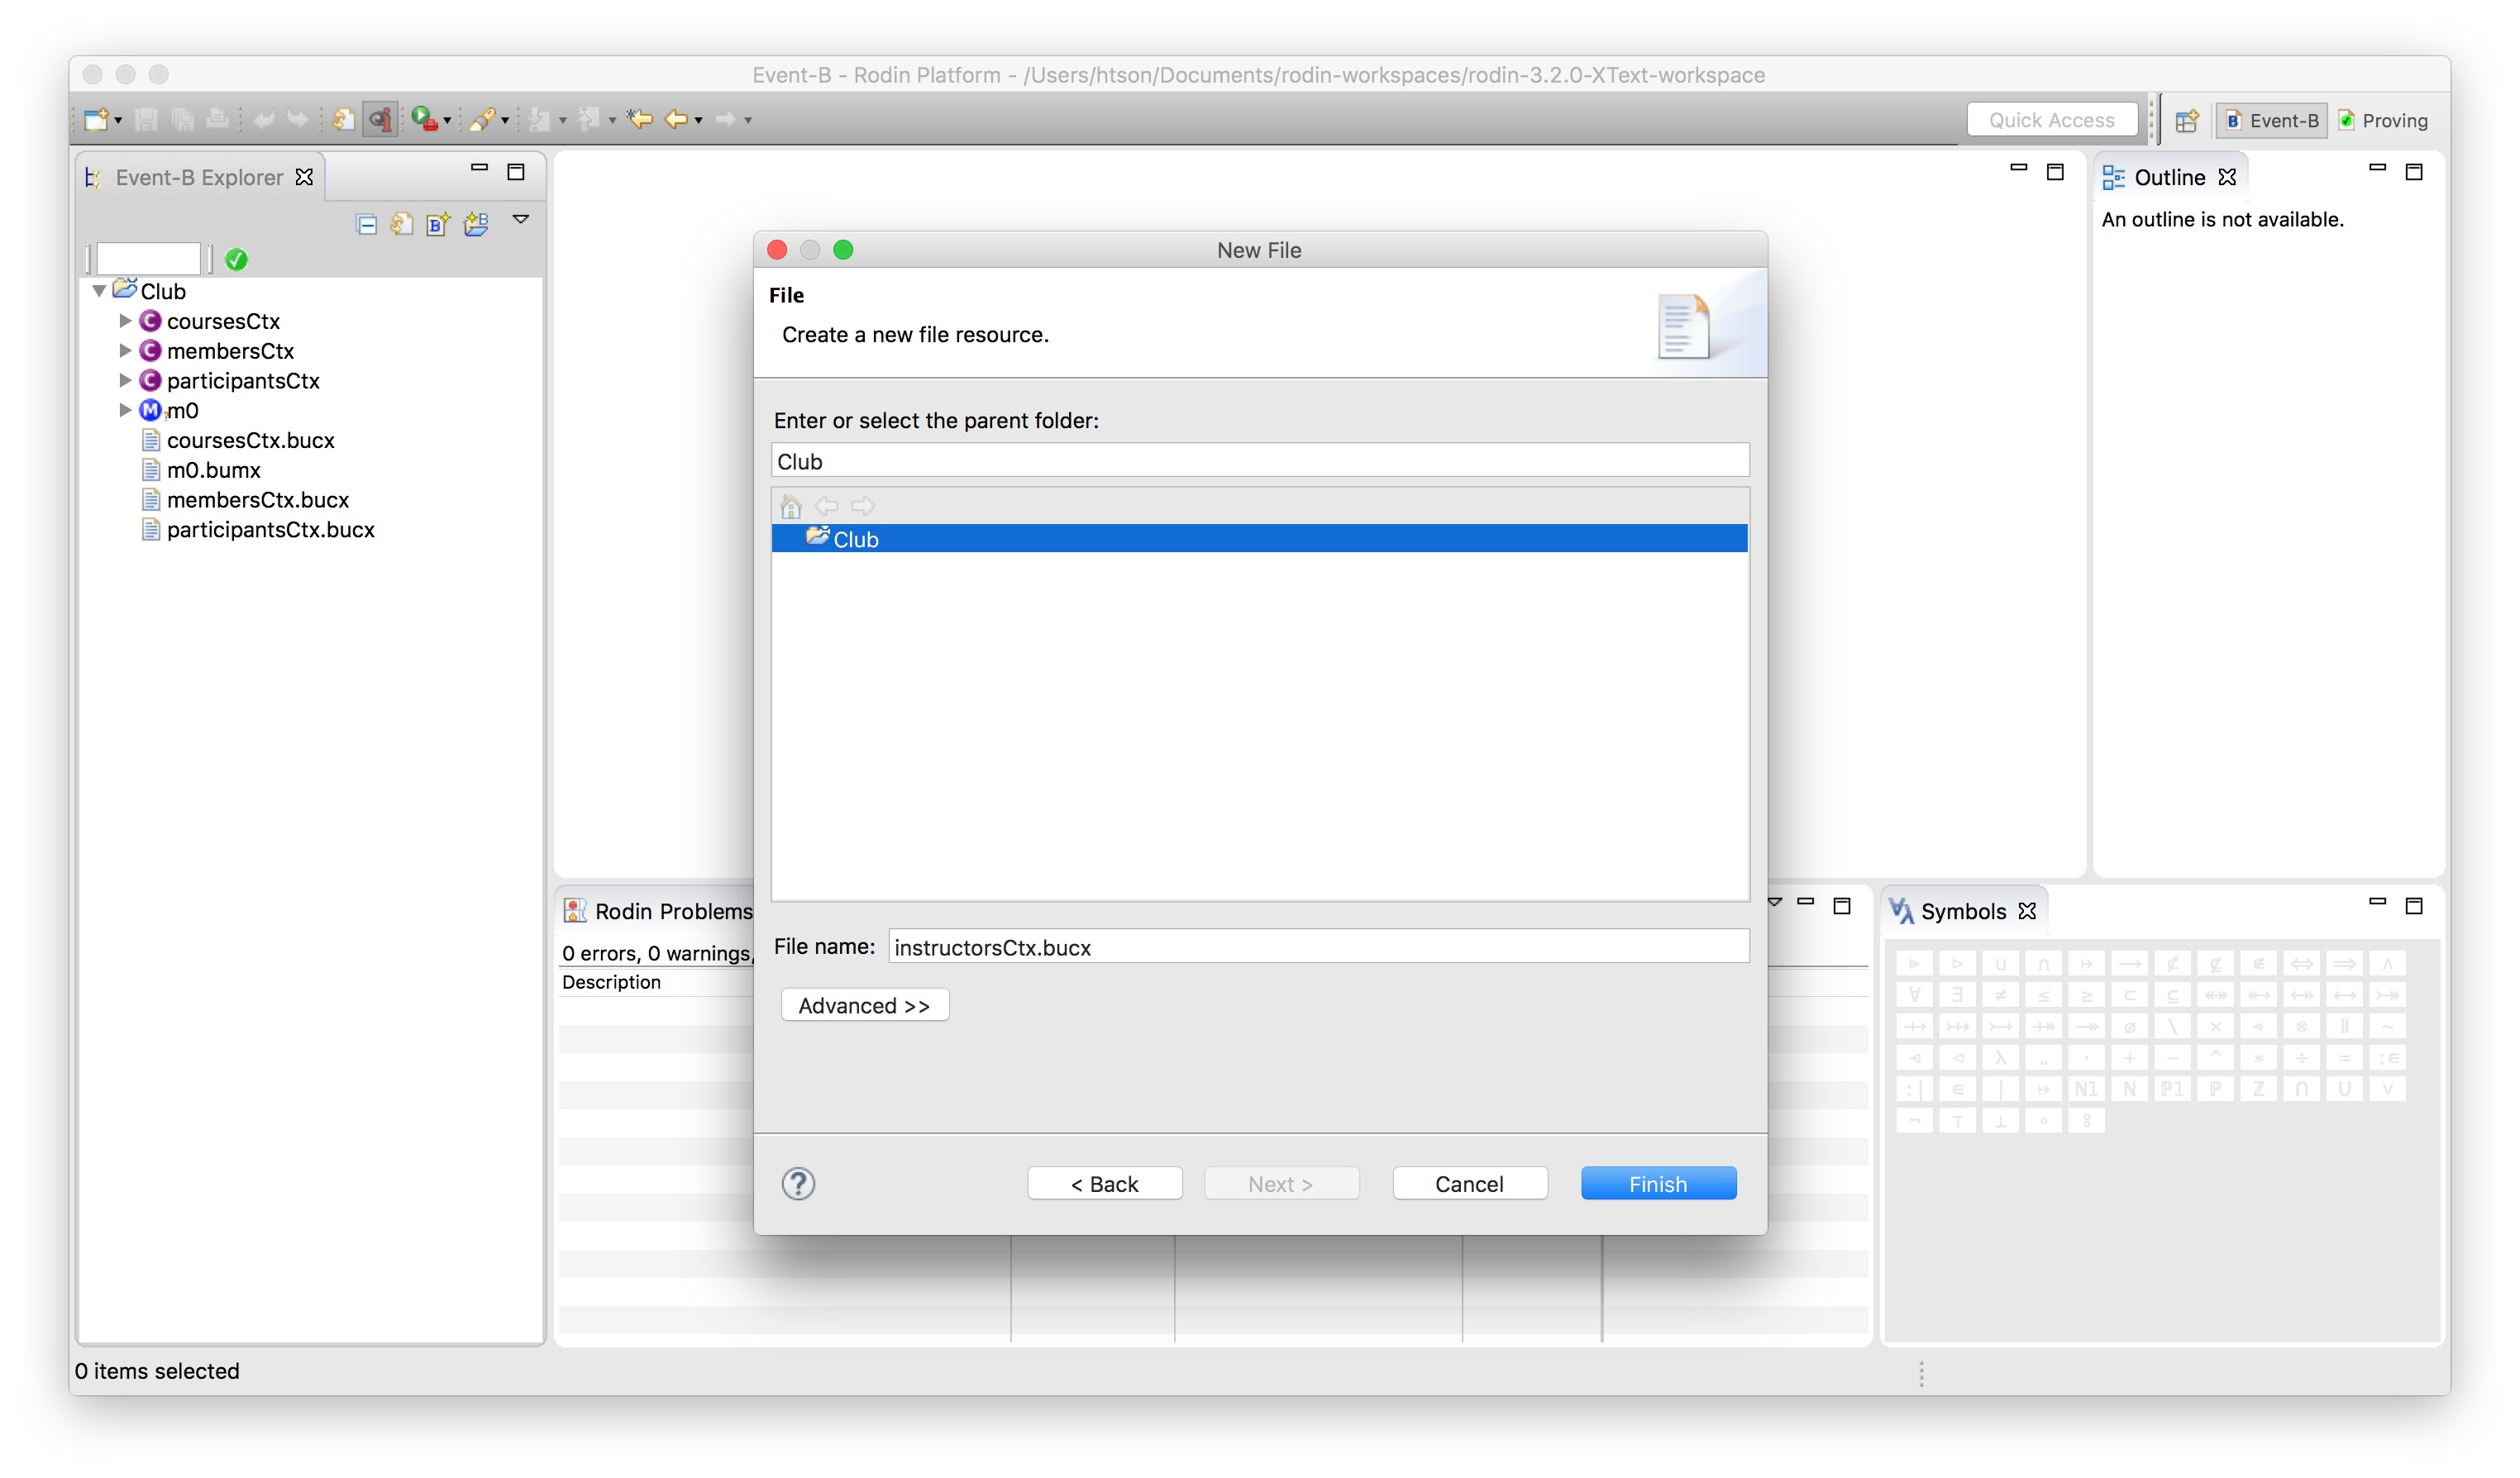
\includegraphics[width=512]{figures/CreateInstructorsCtx}
    \else
    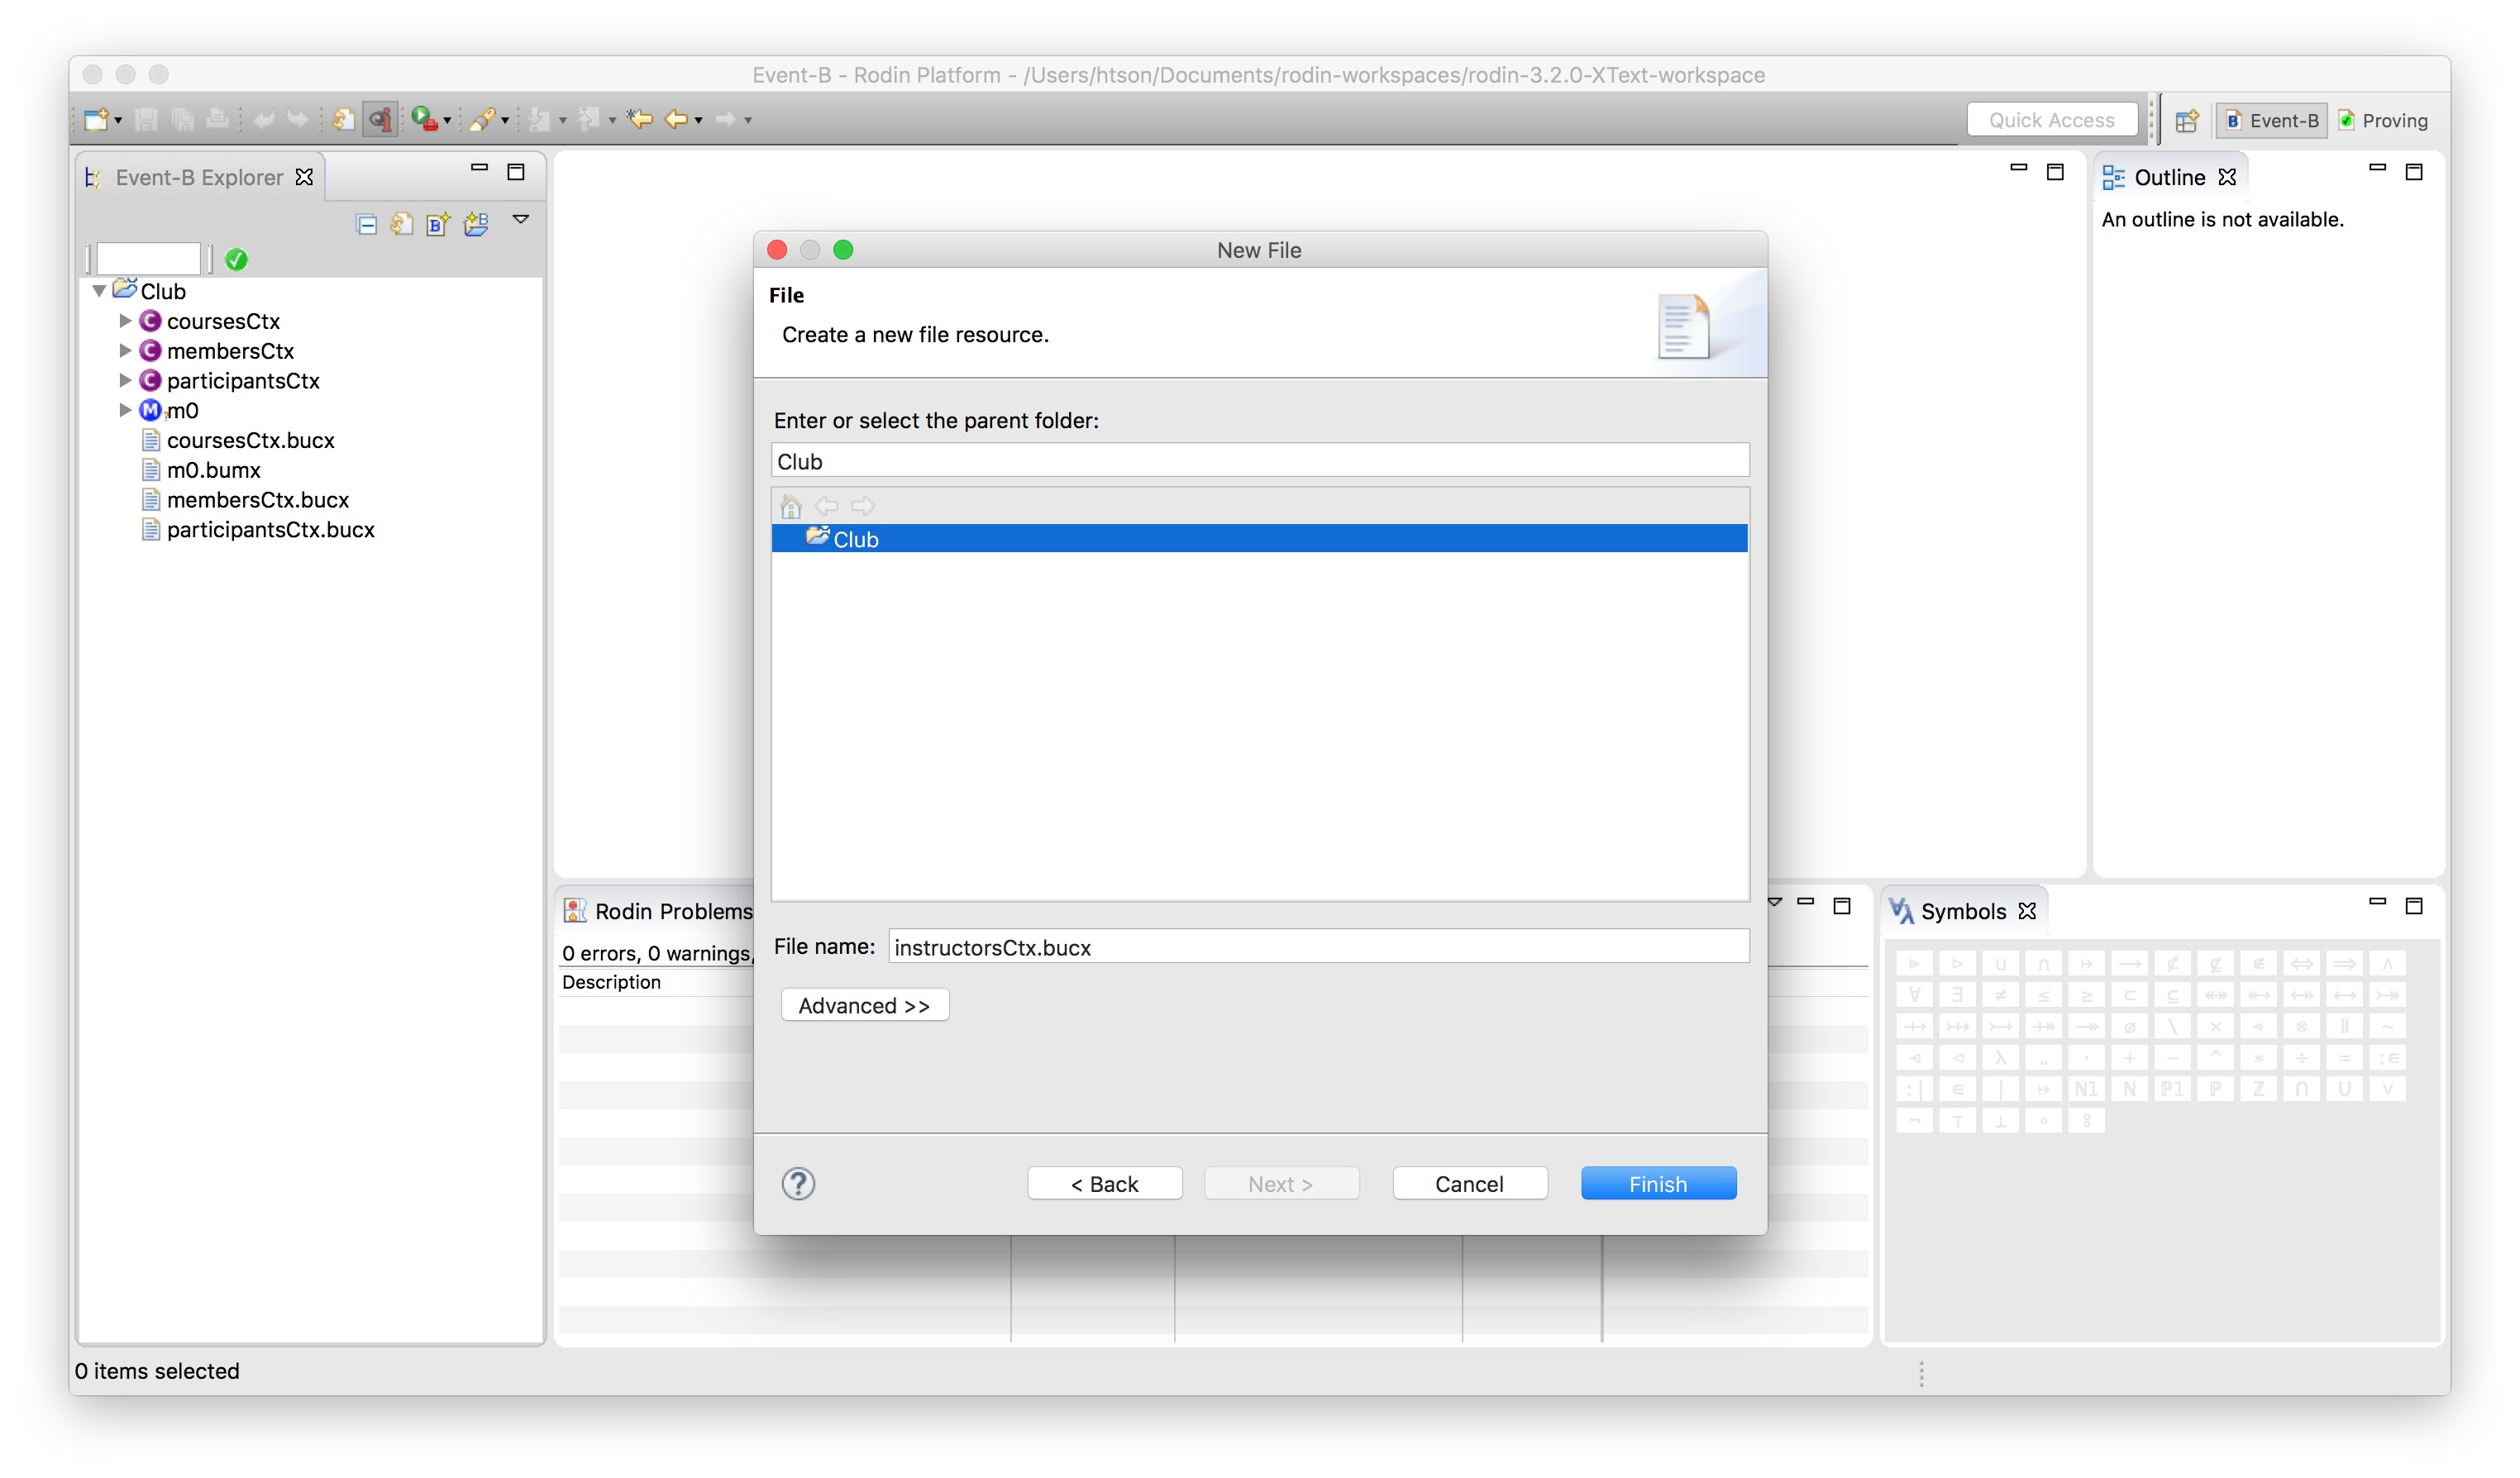
\includegraphics[width=0.9\textwidth]{figures/CreateInstructorsCtx}
    \fi
    \caption{Create instructorsCtx.bucx}
    \label{fig:CreateInstructorsCtx}
  \end{figure}

\item[Step 2. Set the content of instructorsCtx.bucx] \textbf{Set the content of ``instructorsCtx.bucx'' as follows}.
  \begin{center}
    \begin{Bcode}
      \ifplastex
      \Bcontext{} instructorsCtx\\
      \Bextends{} membersCtx coursesCtx\\
      \Bconstants{} INSTR instrs\\
      \Baxioms\\
      @axm1_3: "INSTR ∈ ℙ(MEM)"\\
      @axm1_4: "instrs ∈ CRS → INSTR"\\
      \Bend
      \else
      \Bcontext{} instructorsCtx\\
      \Bextends{} membersCtx coursesCtx\\
      \Bconstants{} INSTR instrs\\
      \Baxioms\\
      \Btab @axm1_3: "\(INSTR \in \pow(MEM)\)"\\
      \Btab @axm1_4: "\(instrs \in CRS \tfun INSTR\)"\\
      \Bend
      \fi
    \end{Bcode}
  \end{center}

\item[Step 3. Auto-format the code] \textbf{Automatically format the content of ``intructorsCtx.bucx''} by using short-cut (e.g., on Mac OS: Cmd+Shift+F).

\item[Step 4. Save the file] \textbf{Save the file ``instructorsCtx.bucx''}.
\end{description}

\textbf{Conclusion} By now, the XContext ``instructorsCtx.bucx'' and the corresponding Rodin Context ``instructorsCtx'' should be visible in the Event-B Explorer (see Figure.
  \begin{figure}[!htbp]
    \centering
    \ifplastex
    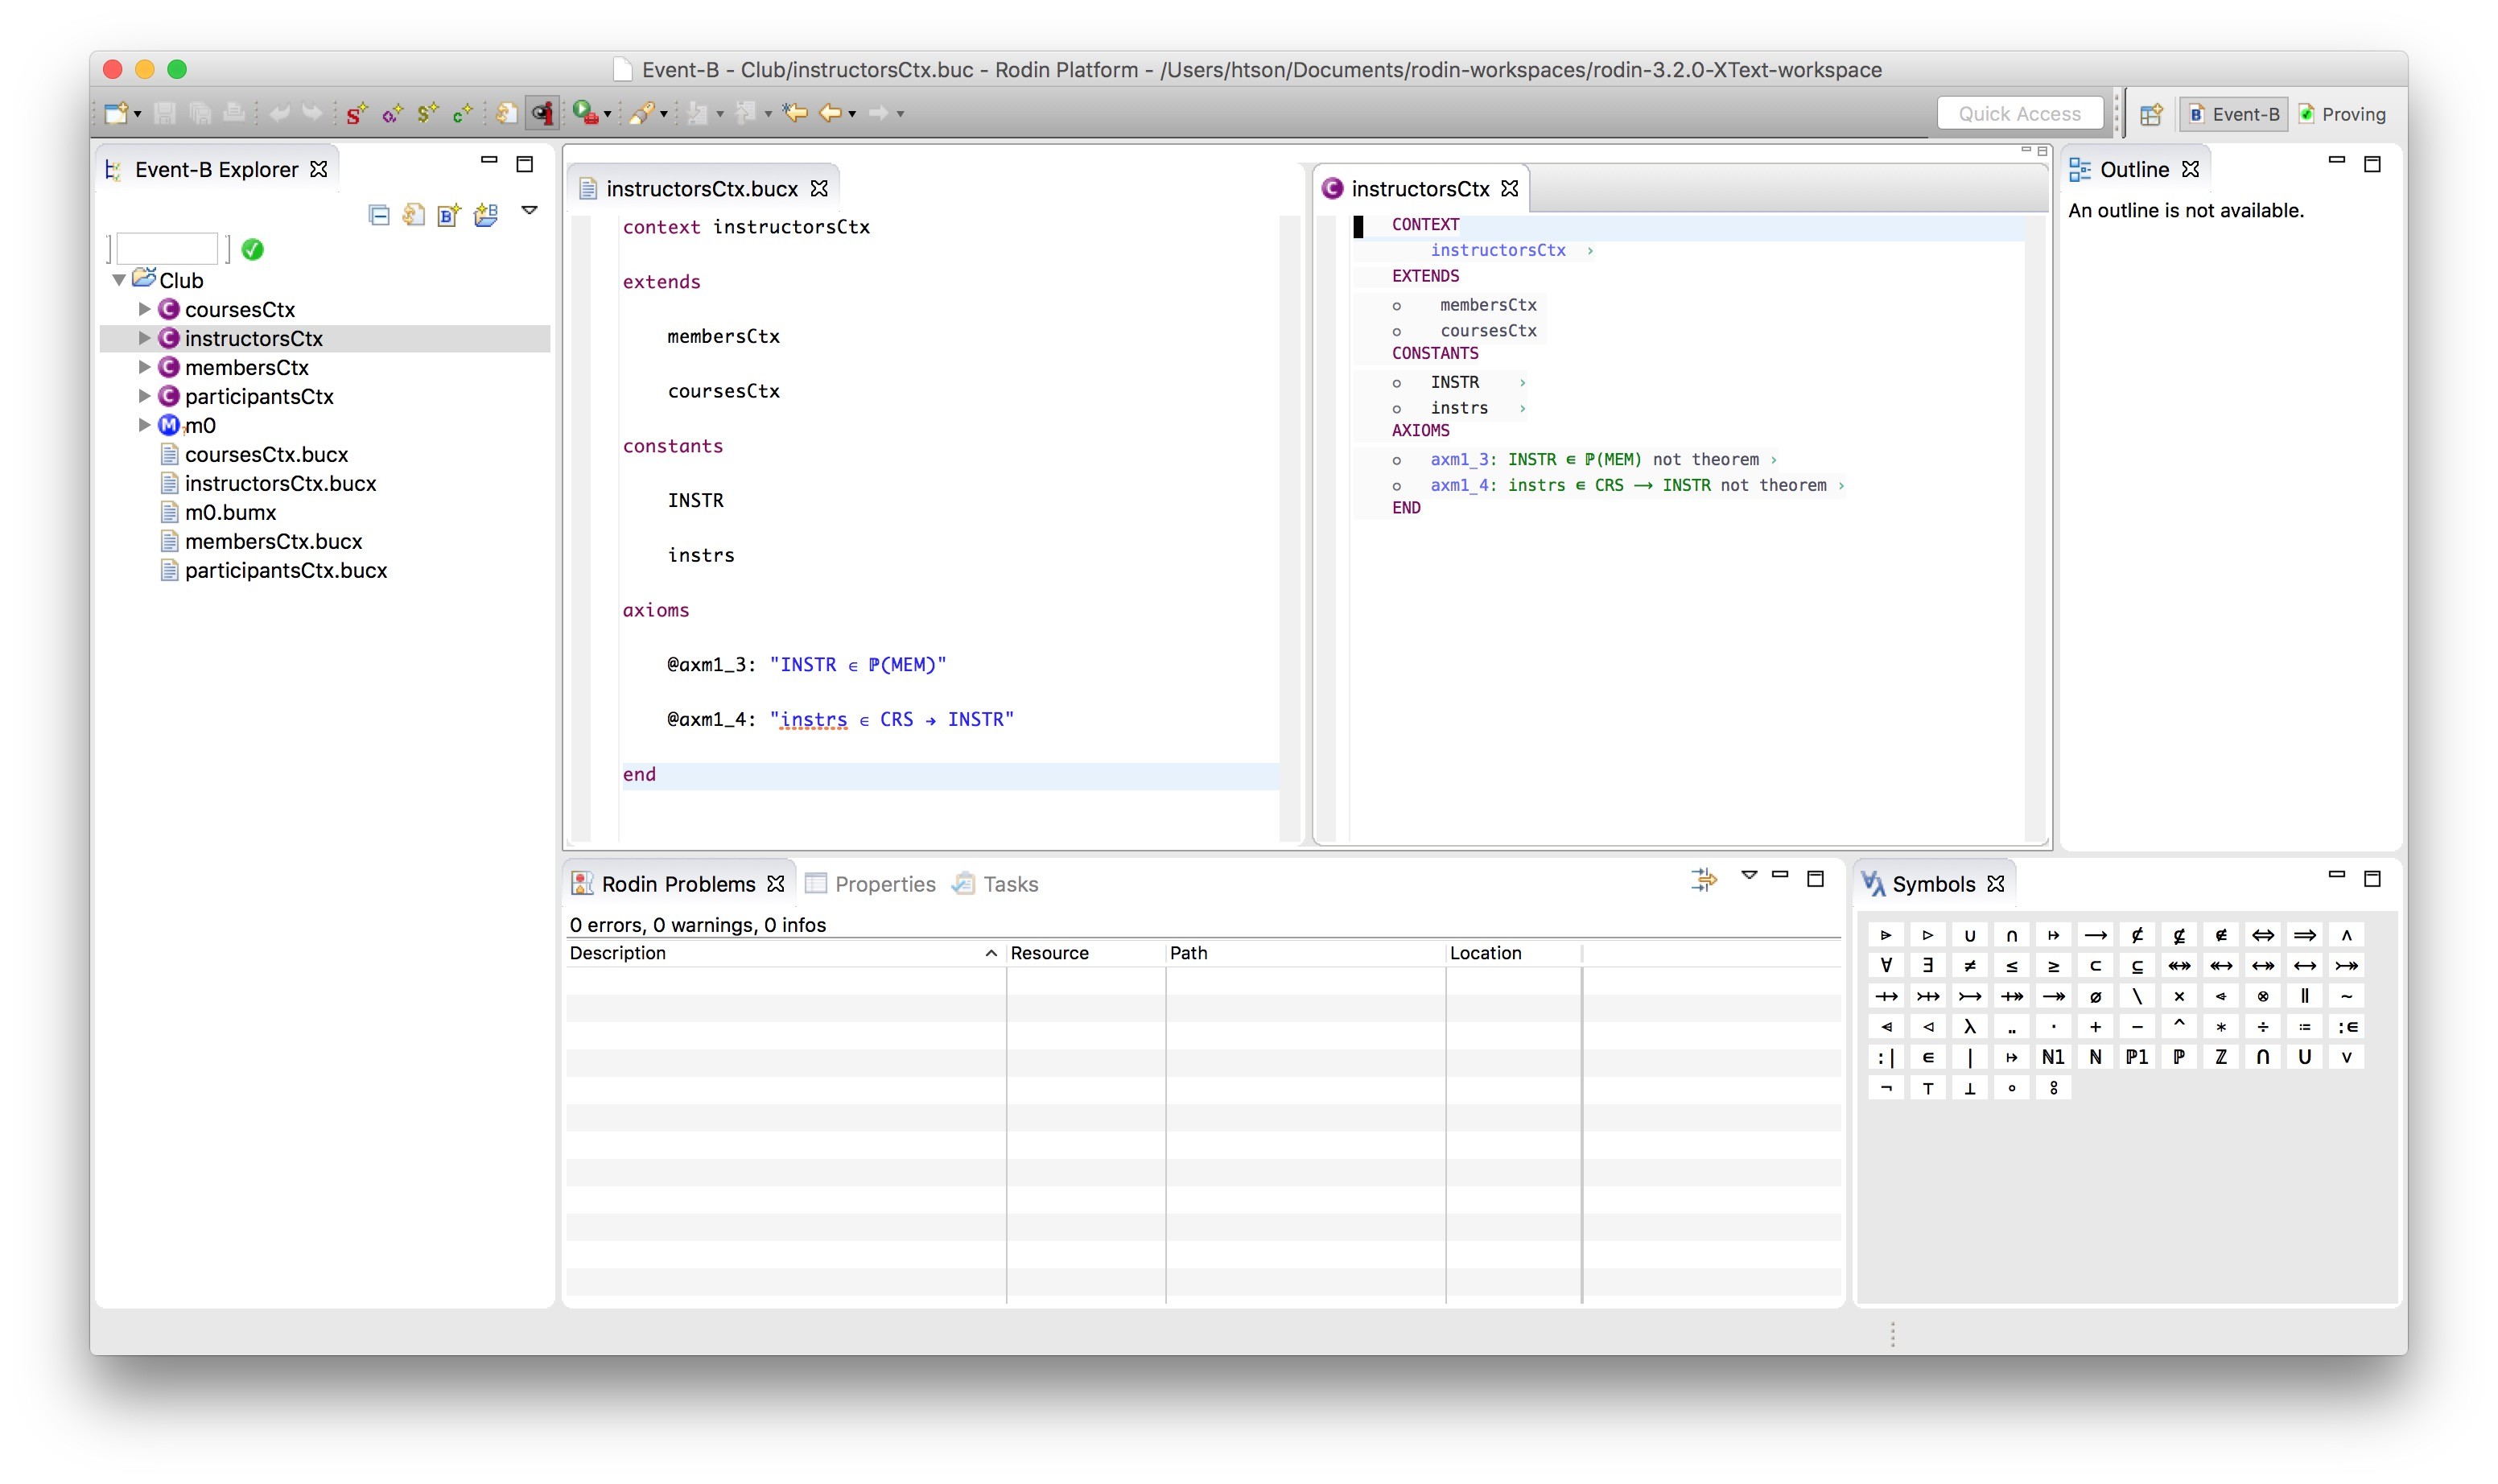
\includegraphics[width=512]{figures/InstructorsCtx}
    \else
    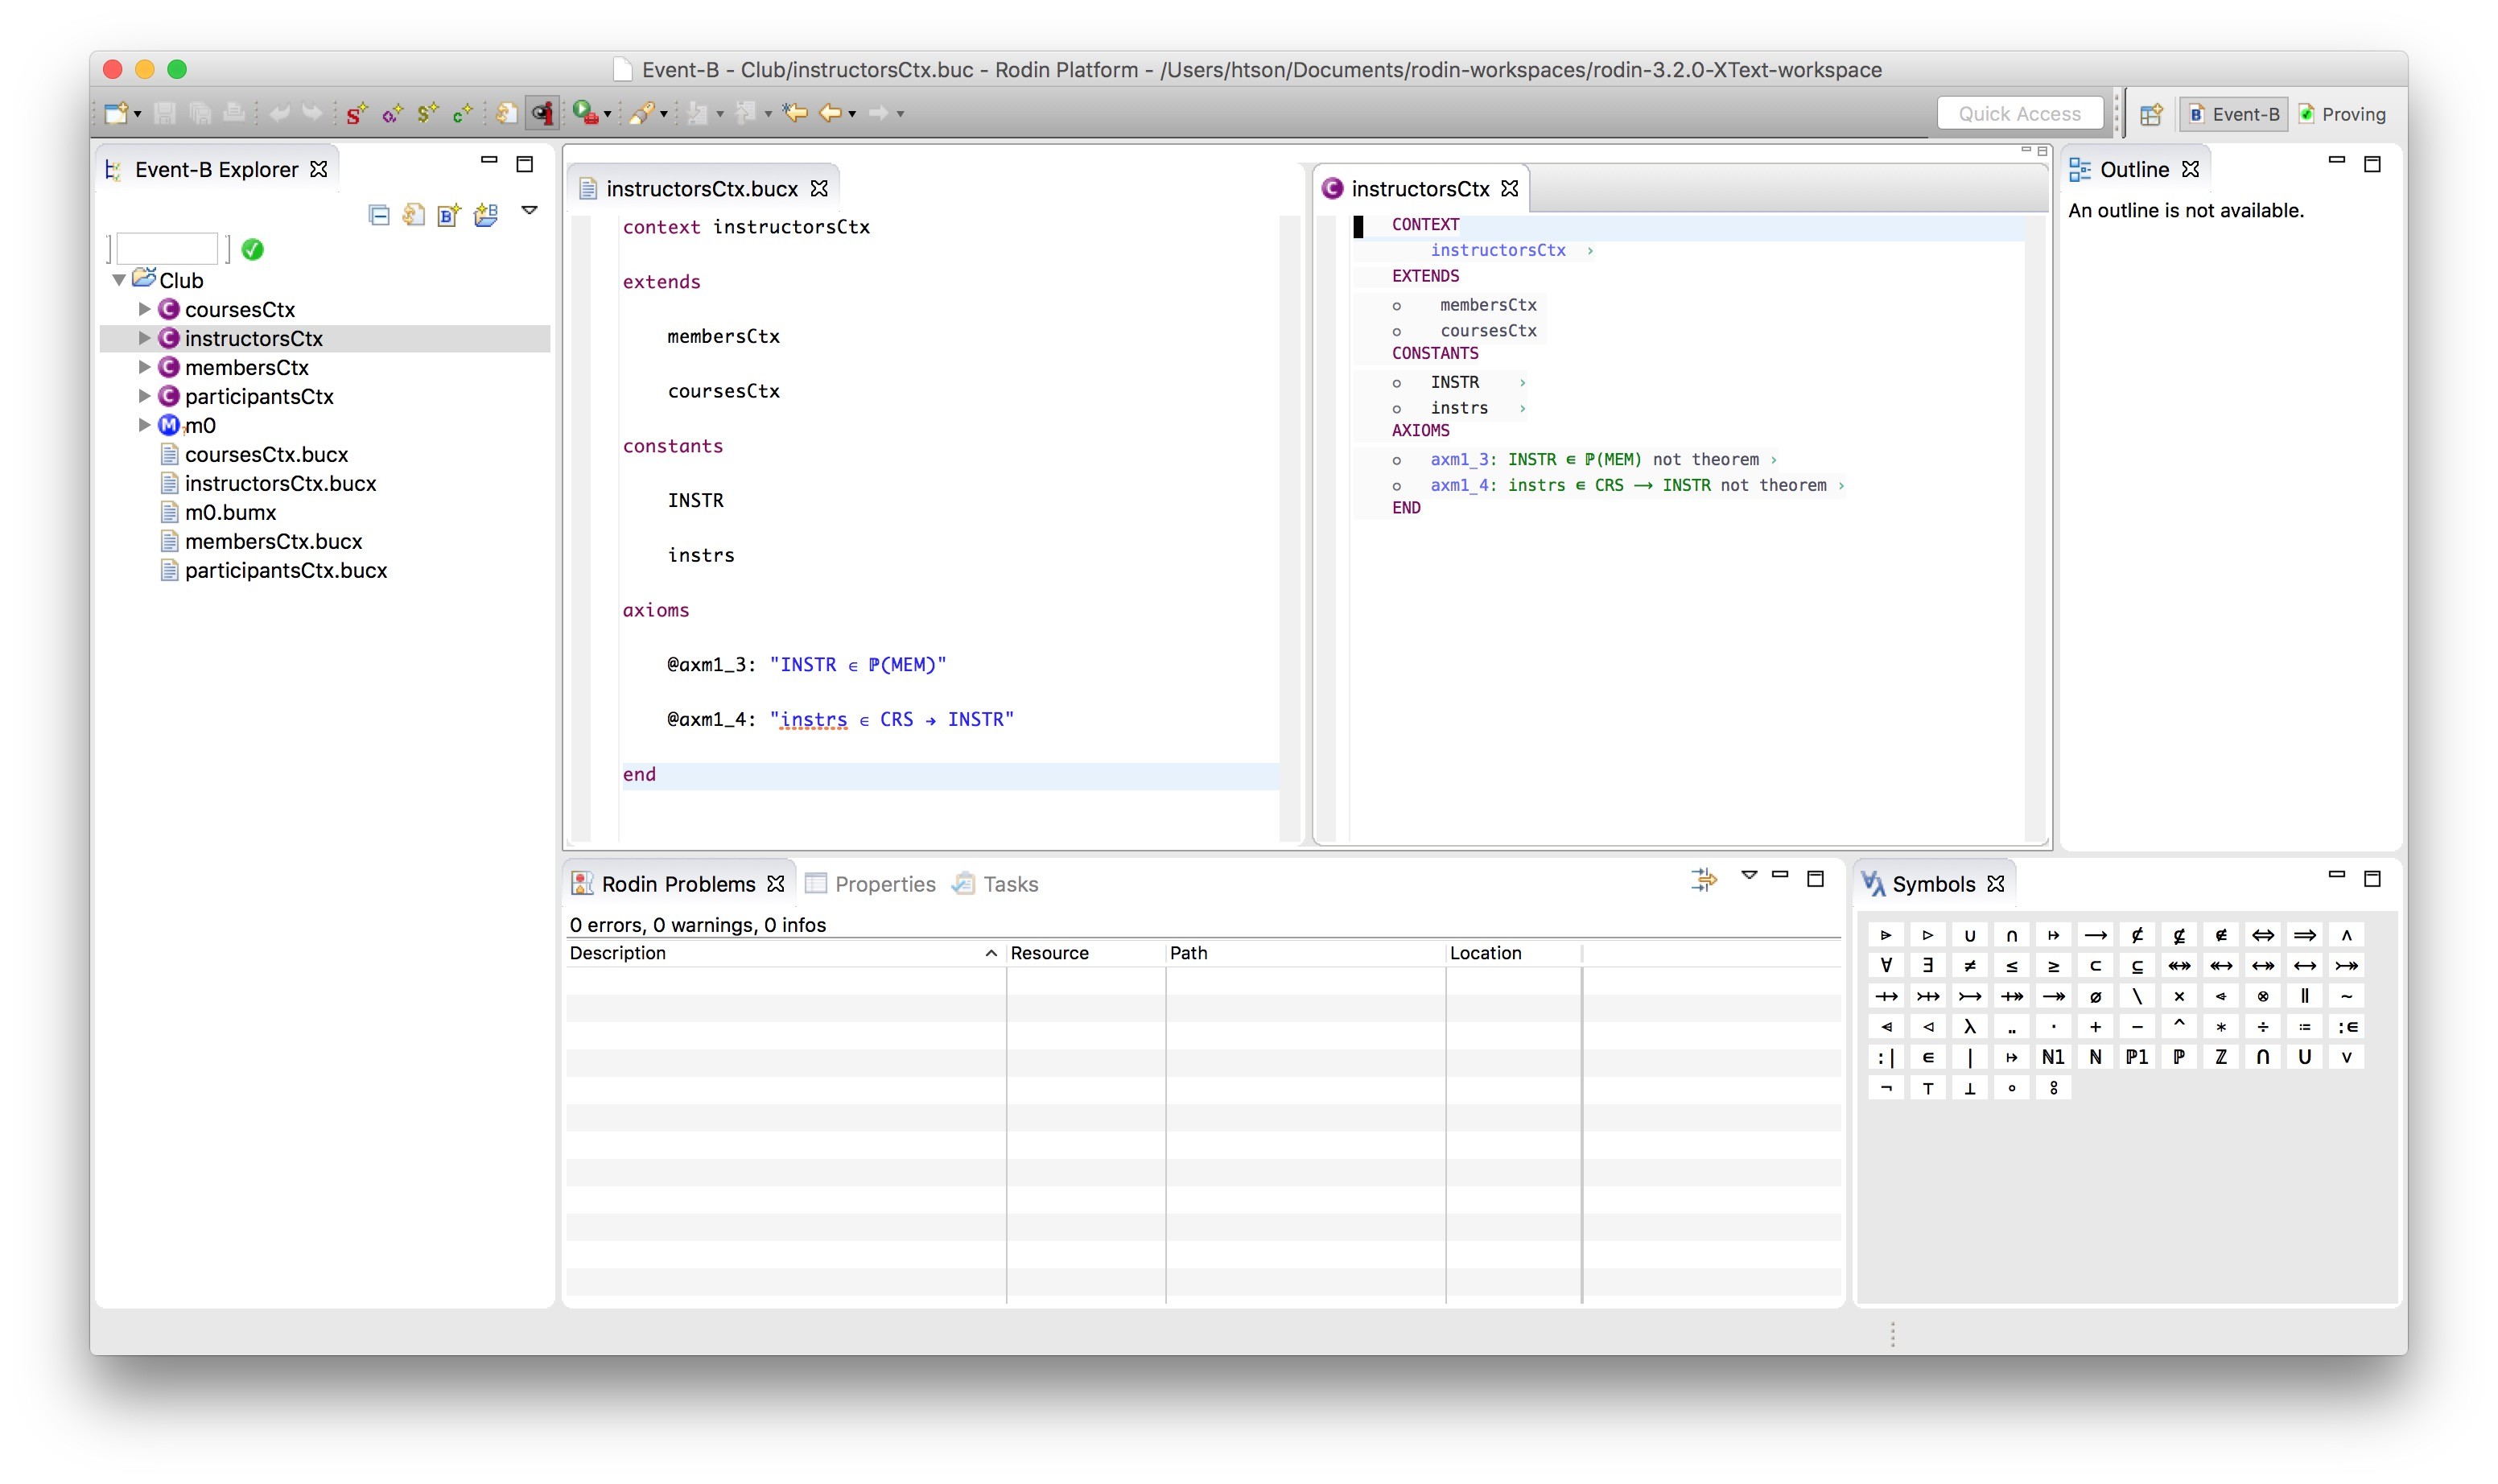
\includegraphics[width=0.9\textwidth]{figures/InstructorsCtx}
    \fi
    \caption{XContext instructorsCtx.bucx}
    \label{fig:instructorsCtx}
  \end{figure}

\subsubsection{Task 6. Create refined XMachines}
\textbf{Introduction} The purpose of this task is to create some more refined XMachines within the ``Club'' project.

\paragraph{Task 6.1. Create a refined XMachine m1.bumx}
\textbf{Introduction} The purpose of this sub-task is to create a refined XMachine ``m1.bumx'' within the ``Club'' project.
\begin{description}
\item[Step 1. Create a new XMachine m1.bumx] \textbf{Create a new XMachine} named ``m1.bumx'' using the \emph{New File wizard} (see Figure~\ref{fig:CreateM1}. The newly created file should be opened automatically in an XMachine editor.
  \begin{figure}[!htbp]
    \centering
    \ifplastex
    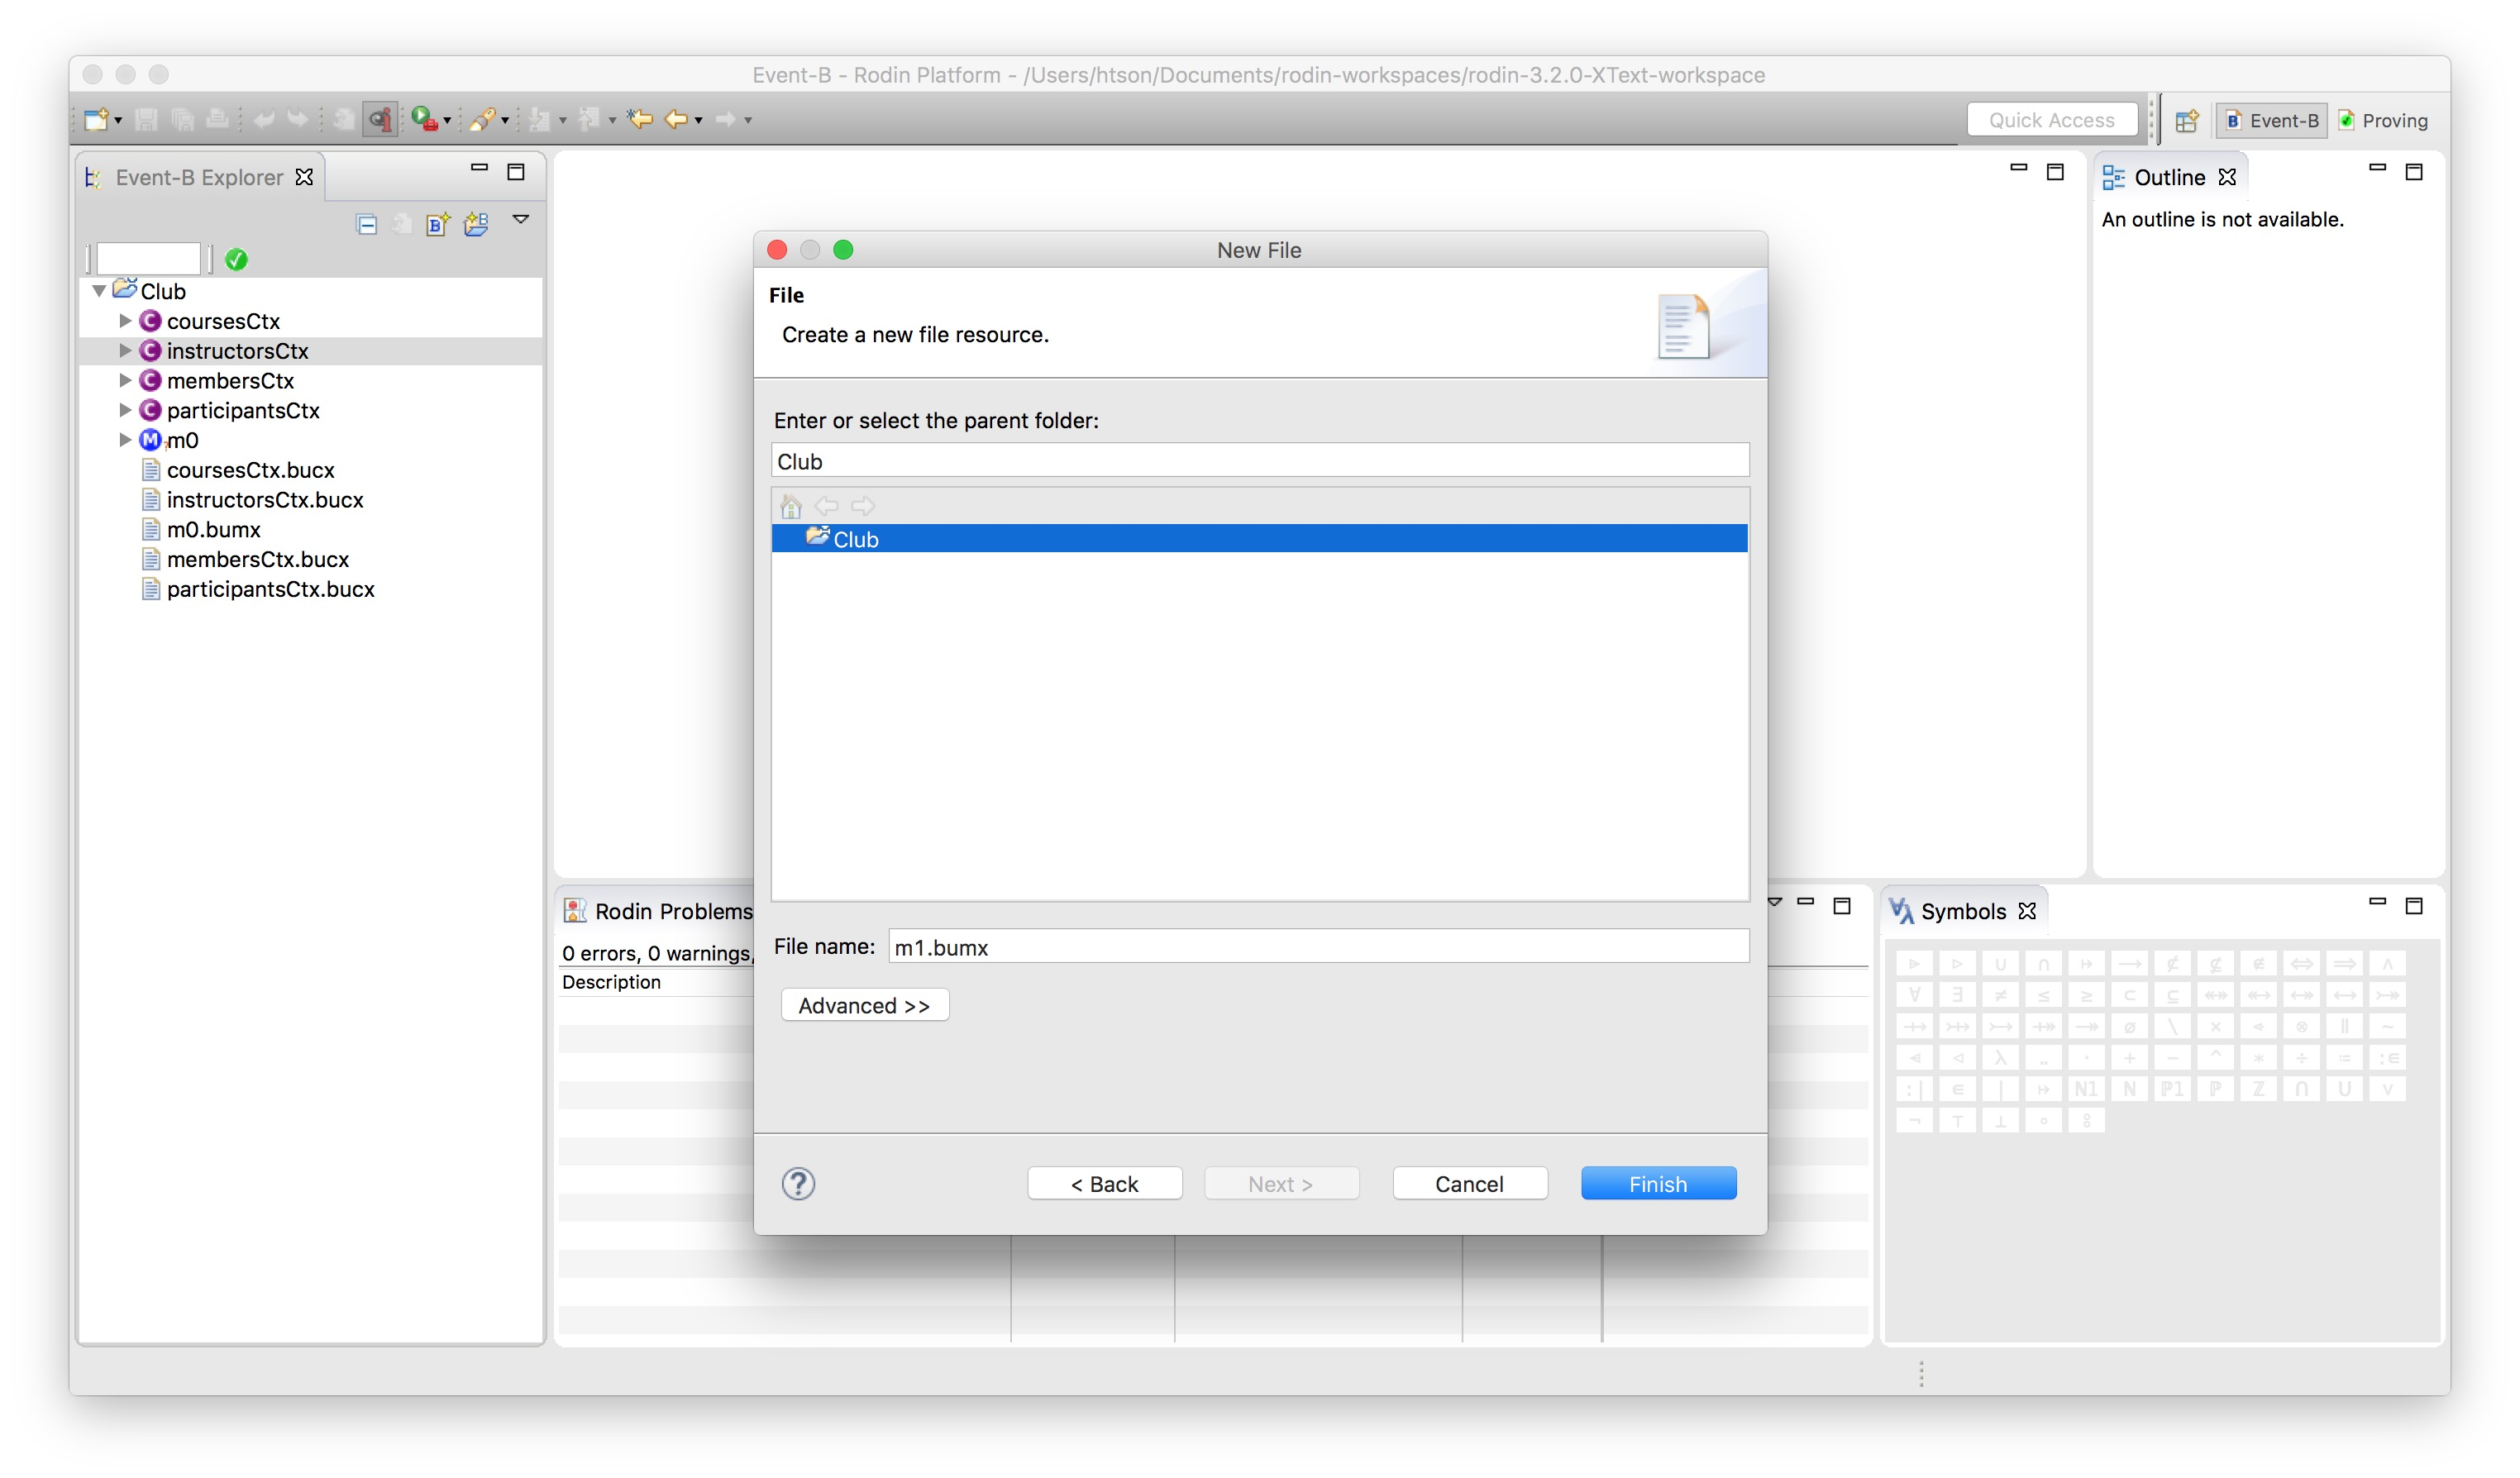
\includegraphics[width=512]{figures/CreateM1}
    \else
    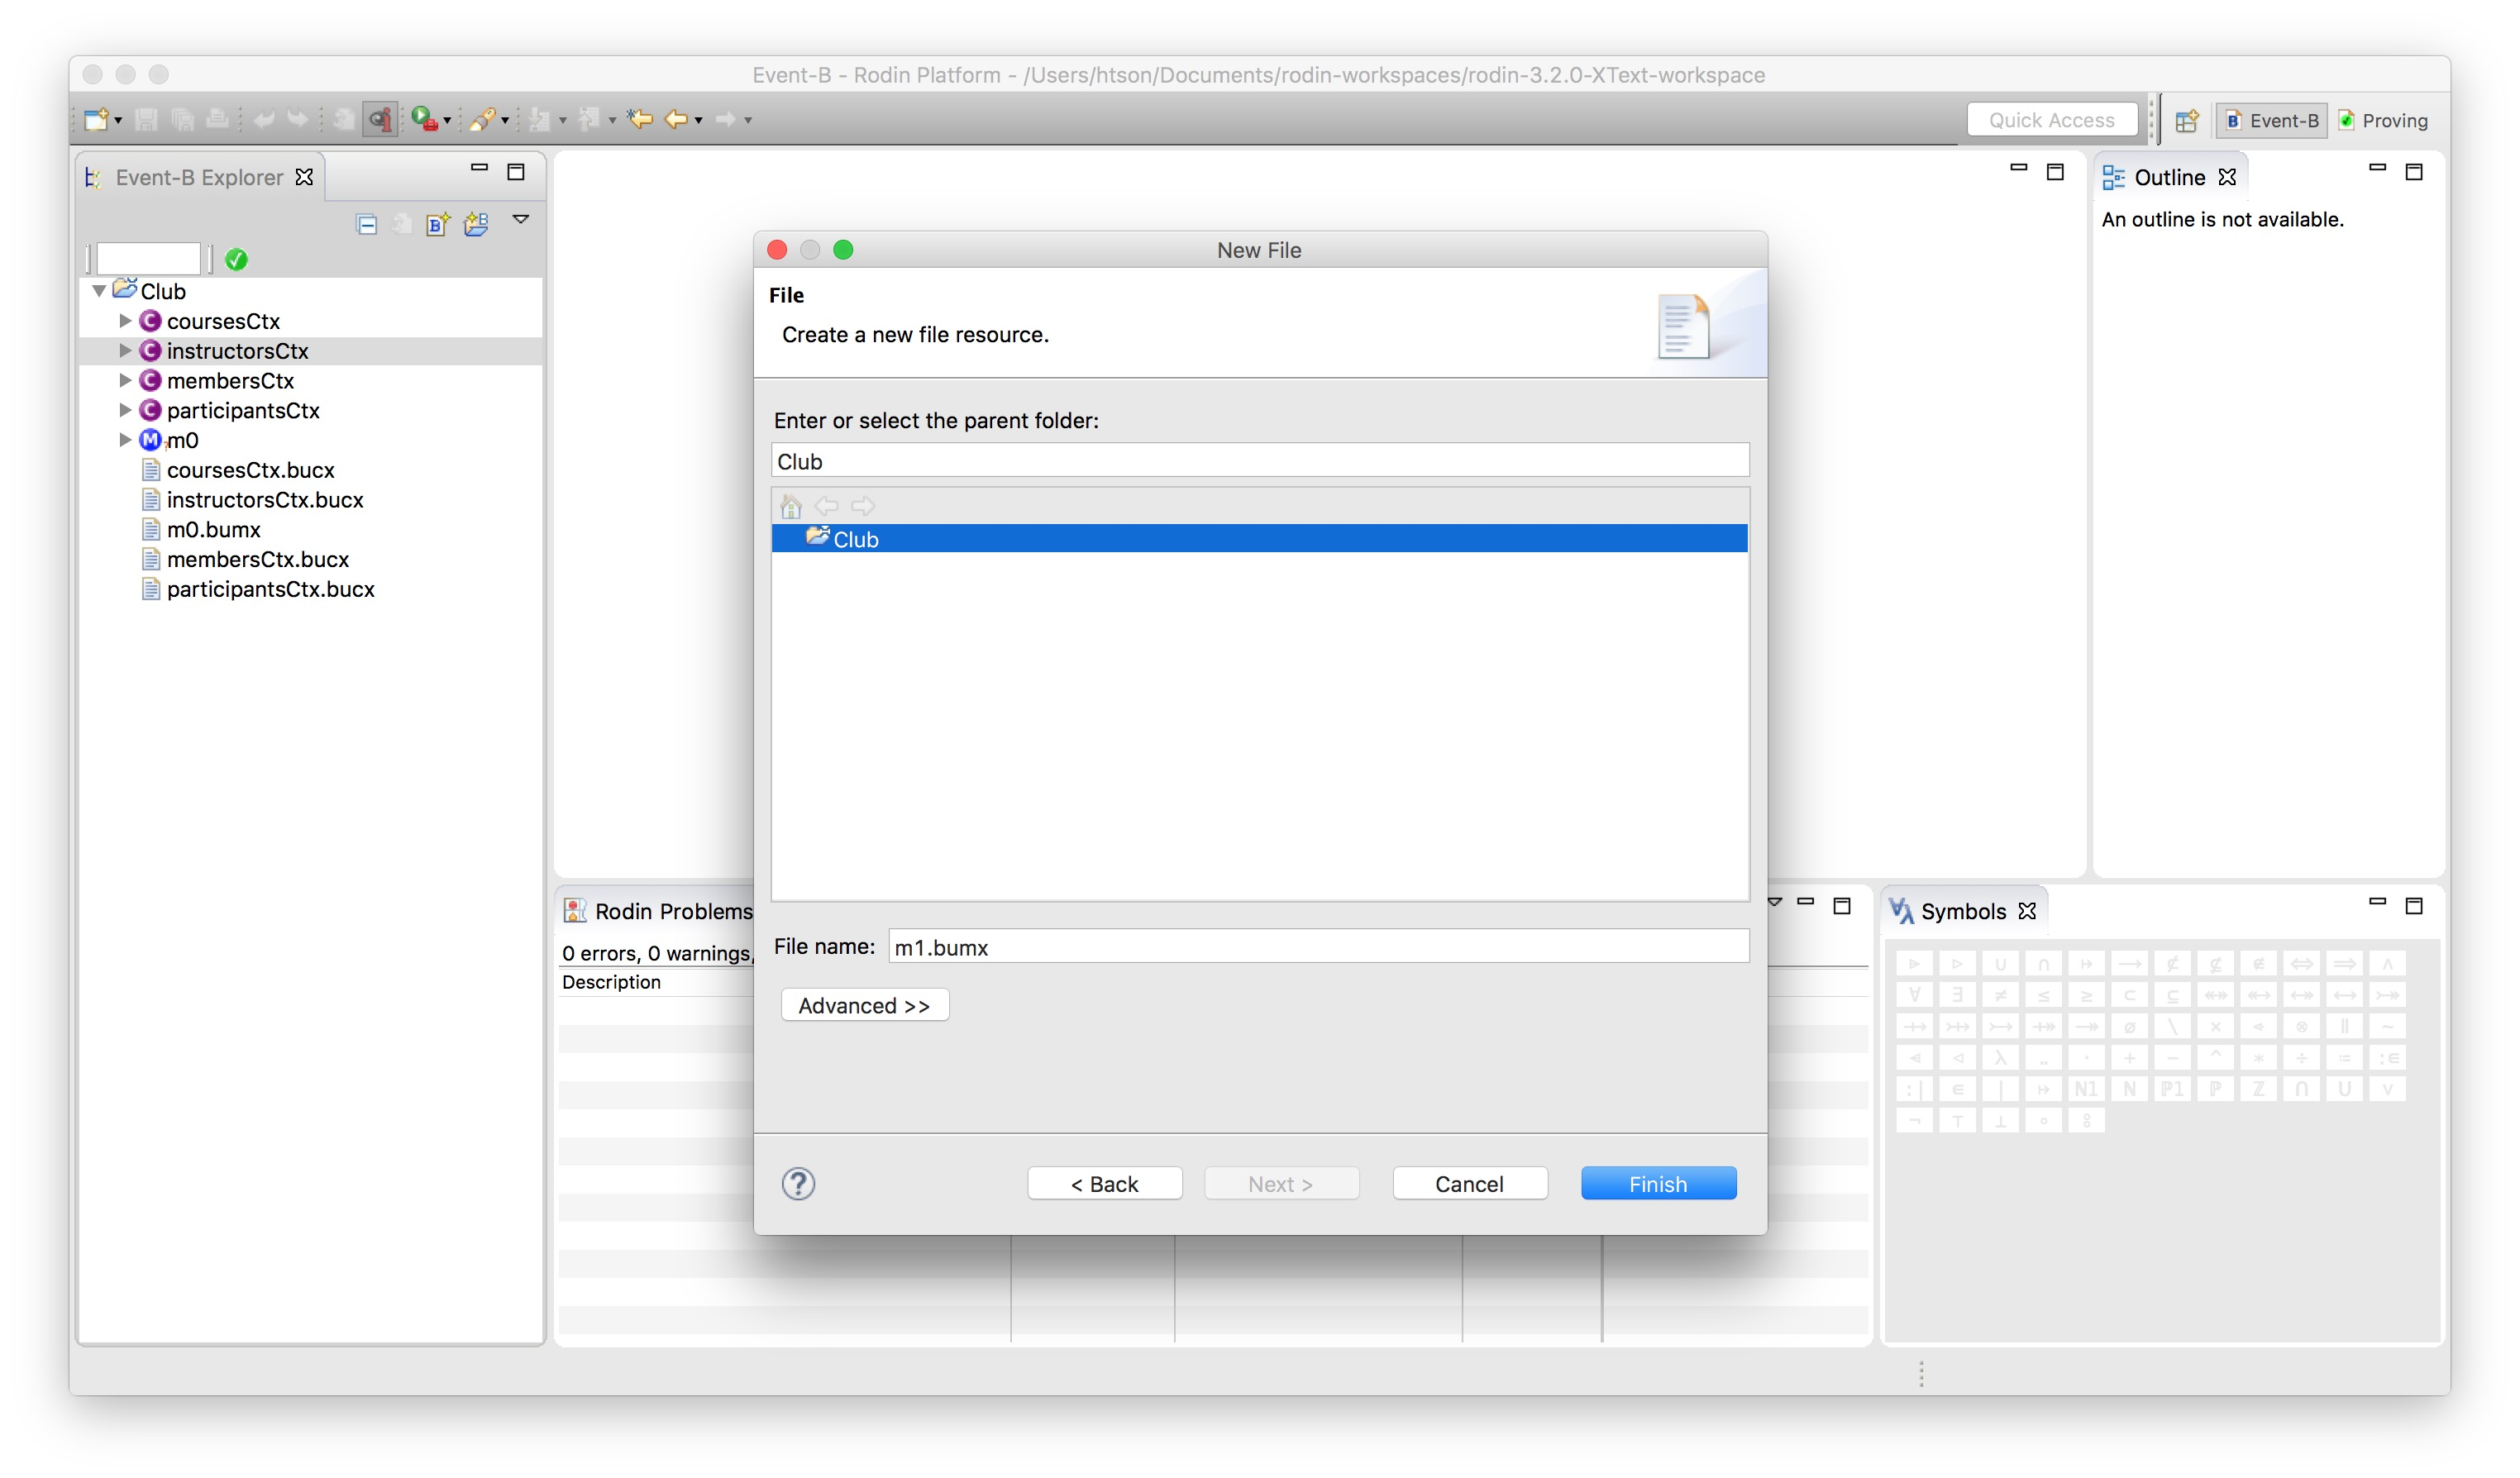
\includegraphics[width=0.9\textwidth]{figures/CreateM1}
    \fi
    \caption{Create m1.bumx}
    \label{fig:CreateM1}
  \end{figure}

\item[Step 2. Set the content of m1.bumx] \textbf{Set the content of ``m1.bumx'' as follows}.
  \begin{center}
    \begin{Bcode}
      \ifplastex
      \Bmachine{} m1\\
      \Brefines{} m0\\
      \Bsees{} instructorsCtx participantsCtx \\
      \Bvariables{} crs prtcpts \\
      \Binvariants\\
      @inv1_1: "prtcpts ∈ crs ↔ PRTCPT"\\
      @inv1_2: "∀c·c ∈ crs ⇒ instrs(c) ∉ prtcpts[\{c\}]"\\
      \Bvariant{} "(crs × PRTCPT) ∖ prtcpts"\\
      \Bevents\\
      INITIALISATION \Bextended\\
      \Bbegin\\
      @act1_2: "prtcpts ≔ ∅"\\
      \Bend\\
      OpenCourses \Bextended\\
      \Brefines{} OpenCourses\\
      \Bwhen\\
      @thm1_2: "dom(prtcpts) ⊆ crs" theorem \\
      \Bend\\
      CloseCourses \Bextended{} \Banticipated\\
      \Brefines{} CloseCourses\\
      \Bbegin\\
      @act1_2: "prtcpts ≔ cs ⩤ prtcpts"\\
      \Bend\\
      Register \Bconvergent\\
      \Bany{} p c \Bwhere \\
      @grd1_1: "p ∈ PRTCPT"\\
      @grd1_2: "c ∈ crs"\\
      @grd1_3: "p ≠ instrs(c)"\\
      @grd1_4: "c ↦ p ∉ prtcpts"\\
      \Bthen\\
      @act1_1: "prtcpts ≔ prtcpts ∪ \{c ↦ p\}"\\
      \Bend\\
      \Bend
      \else
      \Bmachine{} m1\\
      \Brefines{} m0\\
      \Bsees{} instructorsCtx participantsCtx \\
      \Bvariables{} crs prtcpts \\
      \Binvariants\\
      \Btab @inv1_1: "\(prtcpts \in crs \rel PRTCPT\)"\\
      \Btab @inv1_2: "\(\forall c \qdot c ∈ crs \limp instrs(c) \notin prtcpts[\{c\}]\)"\\
      \Bvariant{} "\((crs \cprod PRTCPT) \setminus prtcpts\)"\\
      \Bevents\\
      \Btab INITIALISATION \Bextended\\
      \Btab \Bbegin\\
      \Btab \Btab @act1_2: "\(prtcpts \bcmeq \emptyset\)"\\
      \Btab \Bend\\
      \Btab OpenCourses \Bextended\\
      \Btab \Brefines{} OpenCourses\\
      \Btab \Bwhen\\
      \Btab \Btab @thm1_2: "\(\dom(prtcpts) \subseteq crs\)" theorem \\
      \Btab \Bend\\
      \Btab CloseCourses \Bextended{} \Banticipated\\
      \Btab \Brefines{} CloseCourses\\
      \Btab \Bbegin\\
      \Btab \Btab @act1_2: "\(prtcpts \bcmeq cs \domsub prtcpts\)"\\
      \Btab \Bend\\
      \Btab Register \Bconvergent\\
      \Btab \Bany{} p c \Bwhere \\
      \Btab \Btab @grd1_1: "\(p \in PRTCPT\)"\\
      \Btab \Btab @grd1_2: "\(c \in crs\)"\\
      \Btab \Btab @grd1_3: "\(p \neq instrs(c)\)"\\
      \Btab \Btab @grd1_4: "\(c \mapsto p \neq prtcpts\)"\\
      \Btab \Bthen\\
      \Btab \Btab @act1_1: "\(prtcpts \bcmeq prtcpts \bunion \{c \mapsto p\}\)"\\
      \Btab \Bend\\
      \Bend
      \fi
    \end{Bcode}
  \end{center}

\item[Step 3. Auto-format the code] \textbf{Automatically format the content of ``m1.bumx''} by using short-cut (e.g., on Mac OS: Cmd+Shift+F).

\item[Step 4. Save the file] Save the file ``m1.bumx''.
\end{description}

\textbf{Conclusion} By now, the XMachine ``m1.bucx'' and the corresponding Rodin Machine ``m1'' should be visible in the Event-B Explorer (see Figure~\ref{fig:M1}.
  \begin{figure}[!htbp]
    \centering
    \ifplastex
    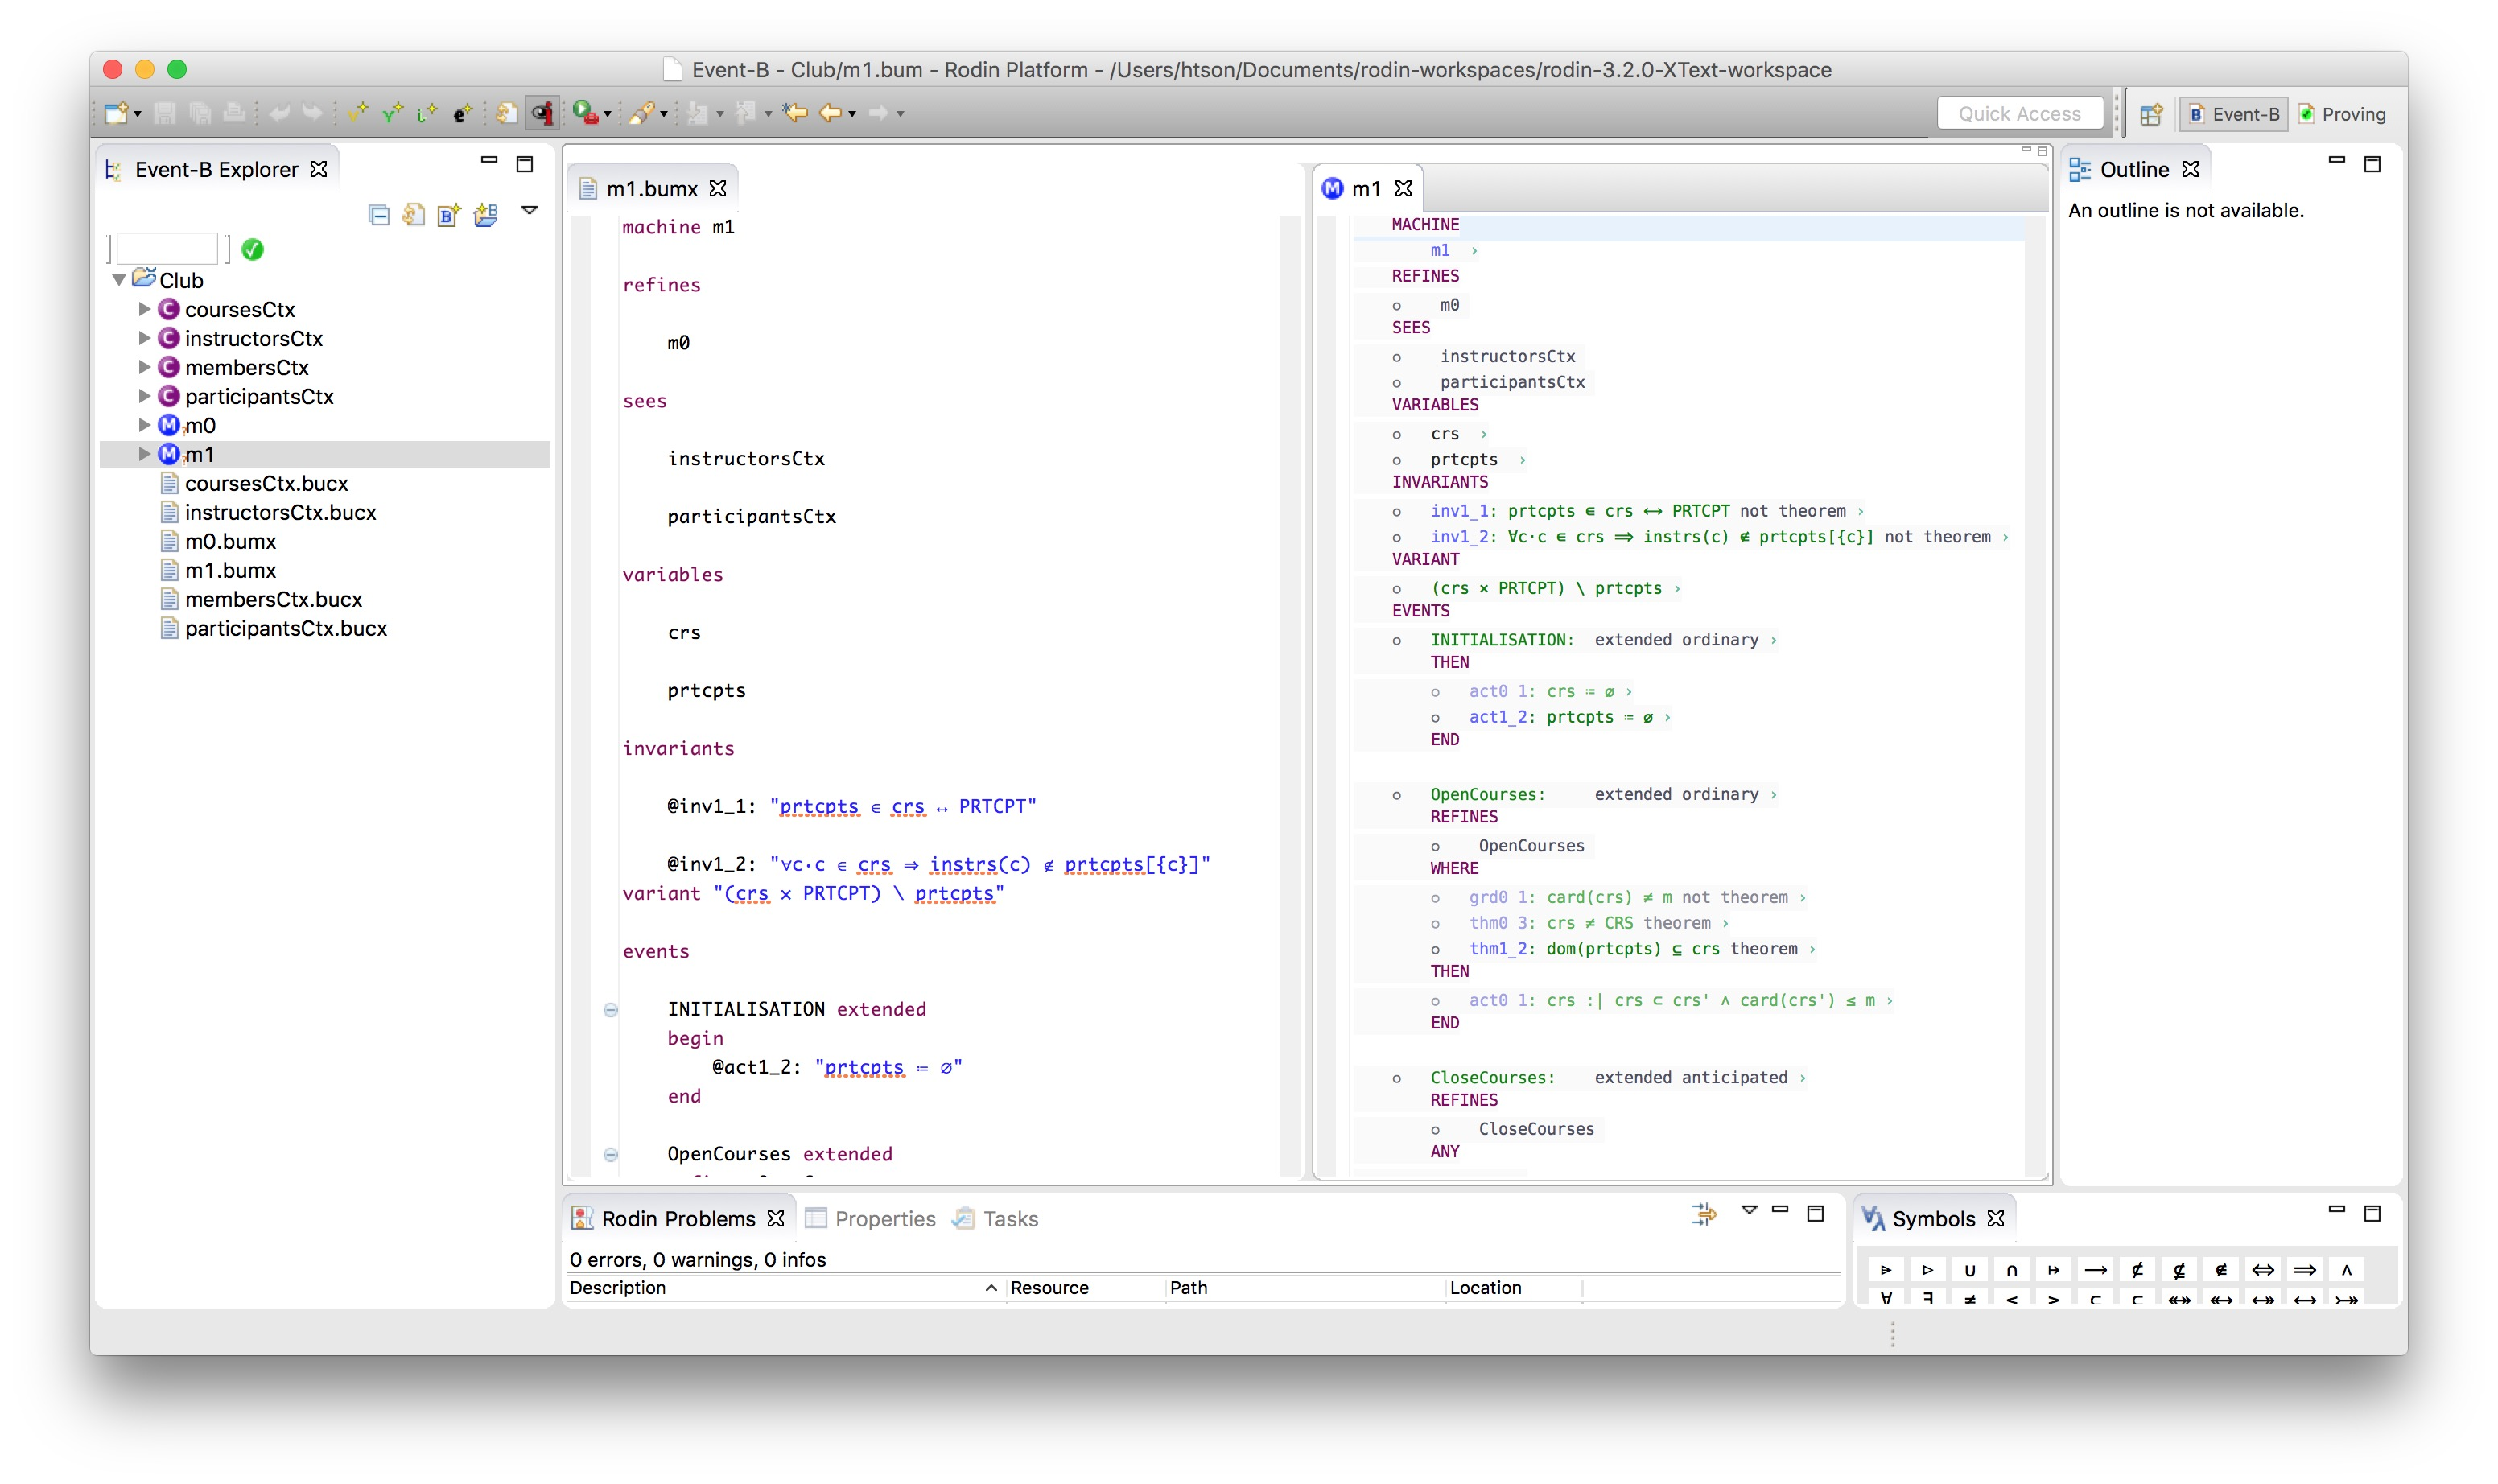
\includegraphics[width=512]{figures/M1}
    \else
    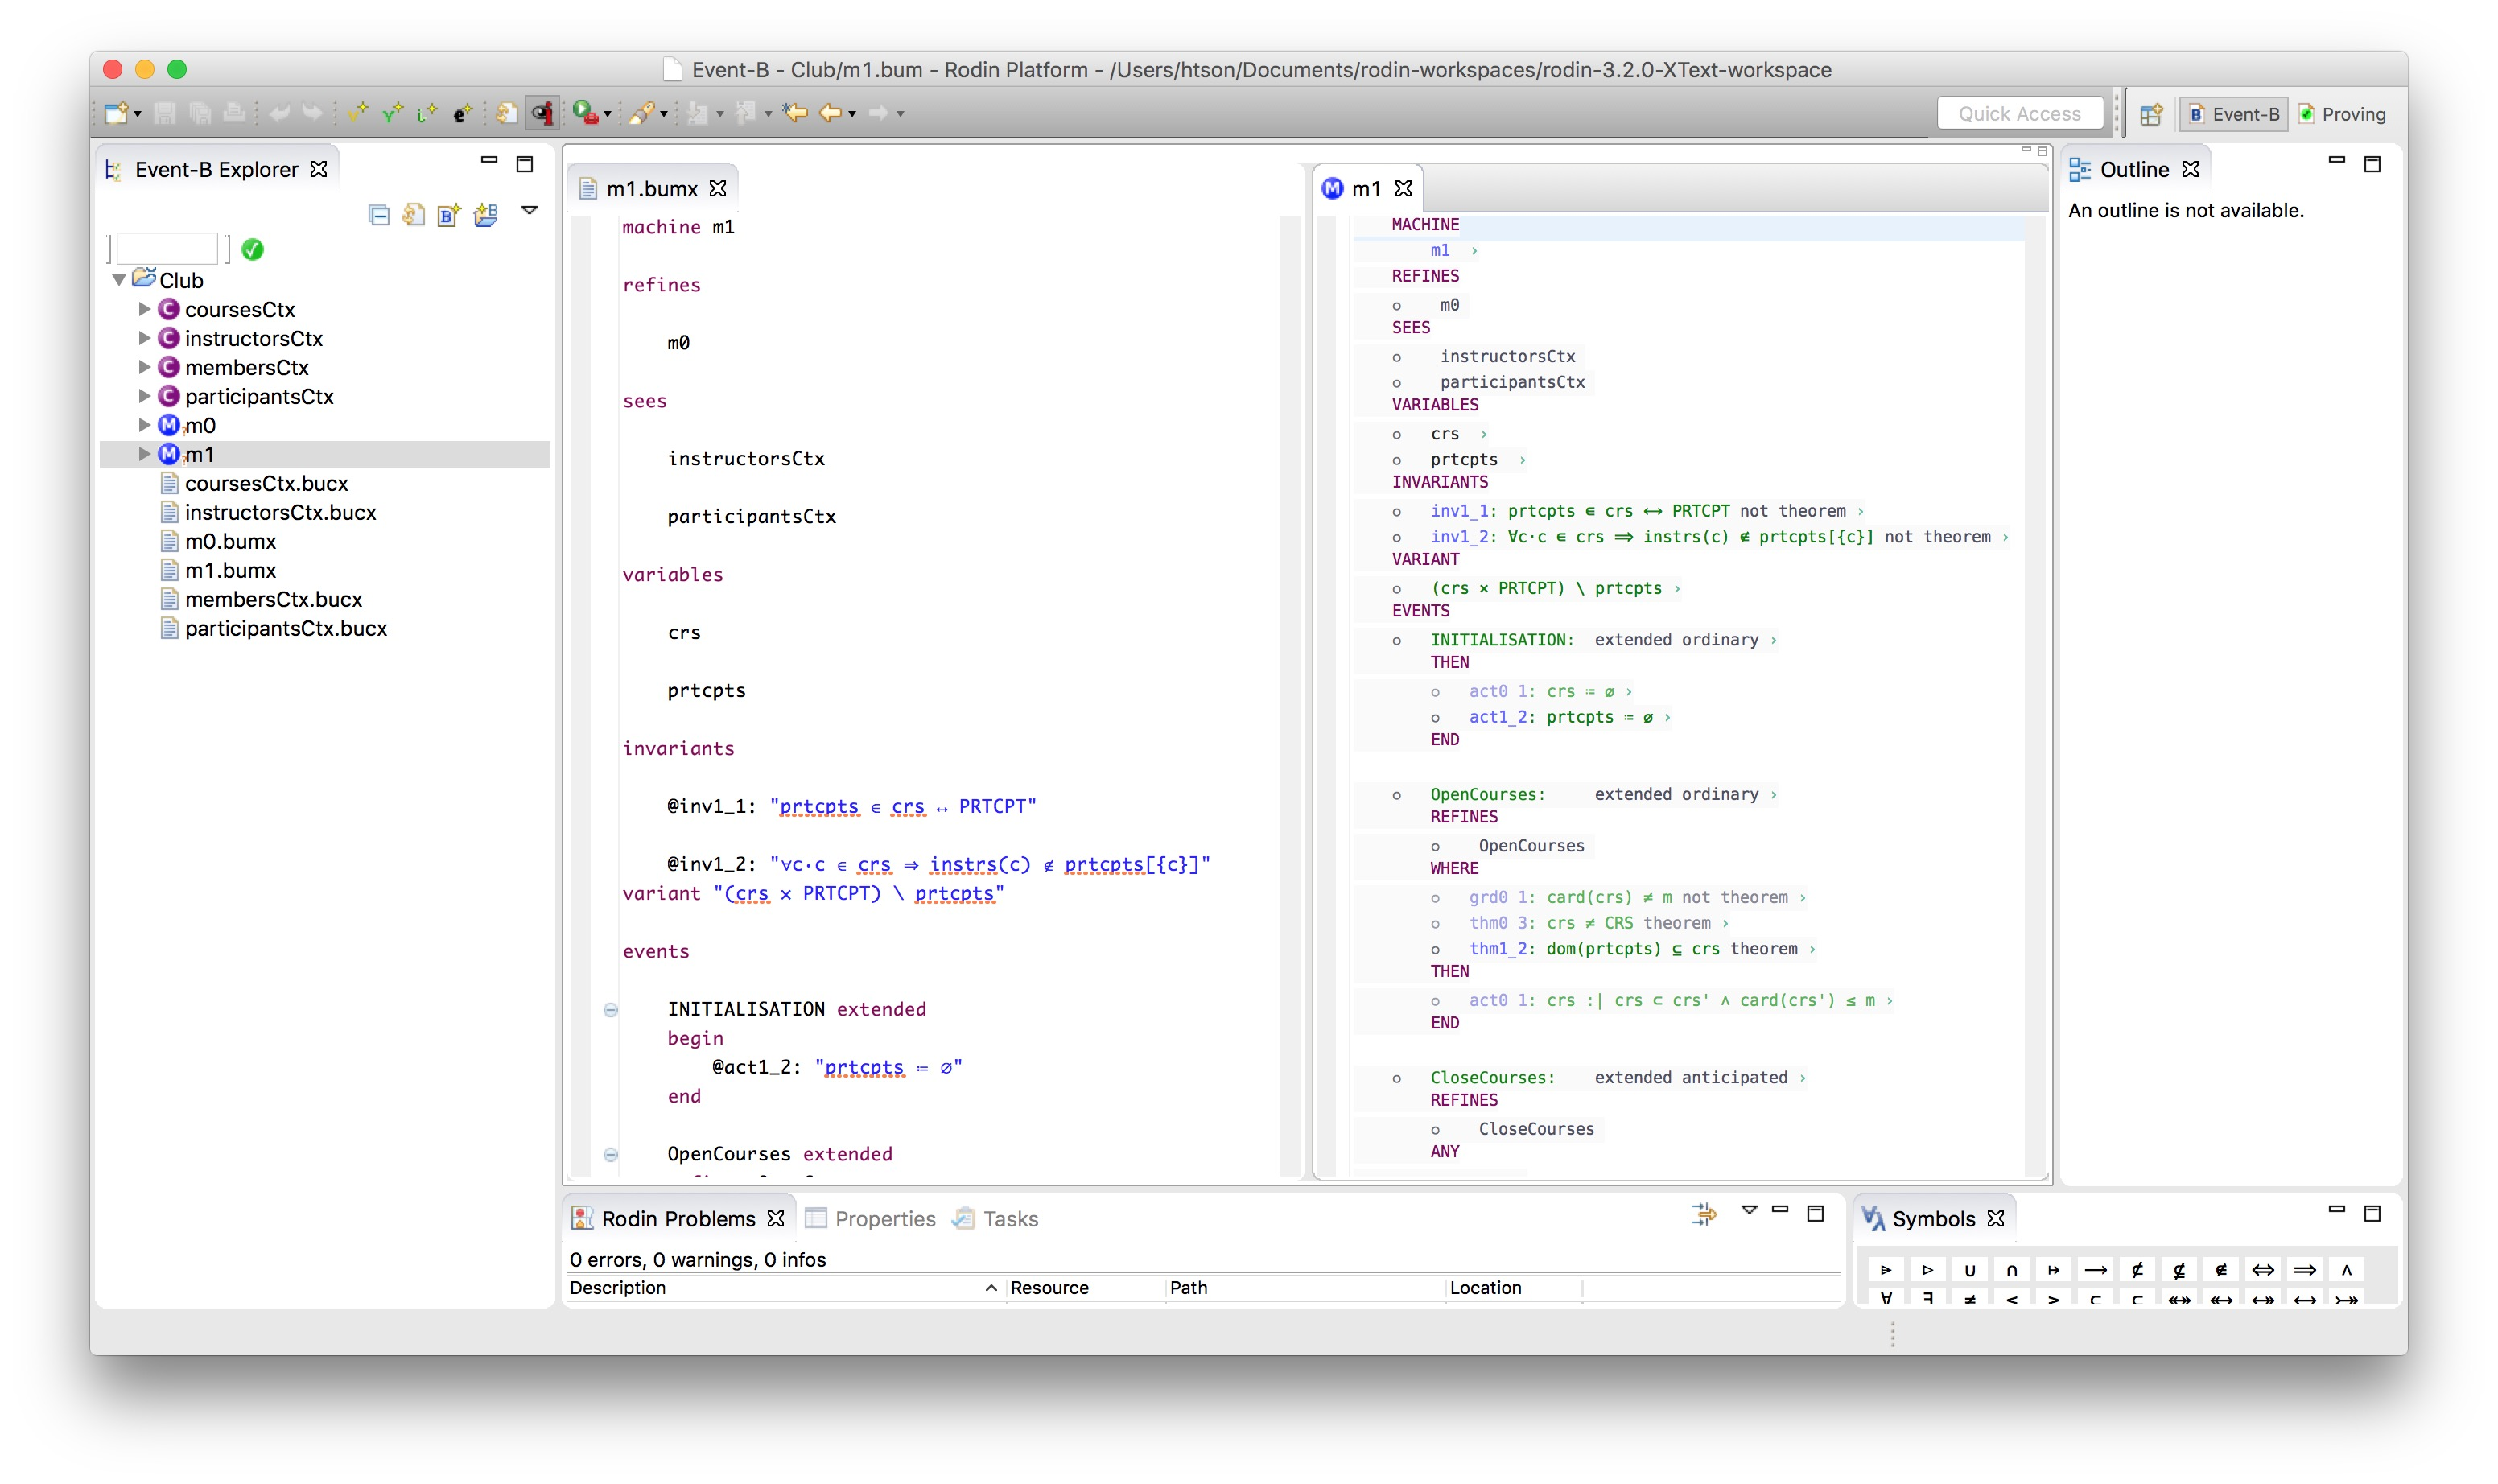
\includegraphics[width=0.9\textwidth]{figures/M1}
    \fi
    \caption{XMachine m1.bumx}
    \label{fig:M1}
  \end{figure}

\paragraph{Task 6.2. Create a refined XMachine m2.bumx}
\textbf{Introduction} The purpose of this sub-task is to create a refined XMachine ``m2.bumx'' within the ``Club'' project.

\begin{description}
\item[Step 1. Create a new XMachine m2.bumx] \textbf{Create a new XMachine} named ``m2.bumx'' using the \emph{New File wizard} (see Figure~\ref{fig:CreateM2}. The newly created file should be opened automatically in an XMachine editor.
  \begin{figure}[!htbp]
    \centering
    \ifplastex
    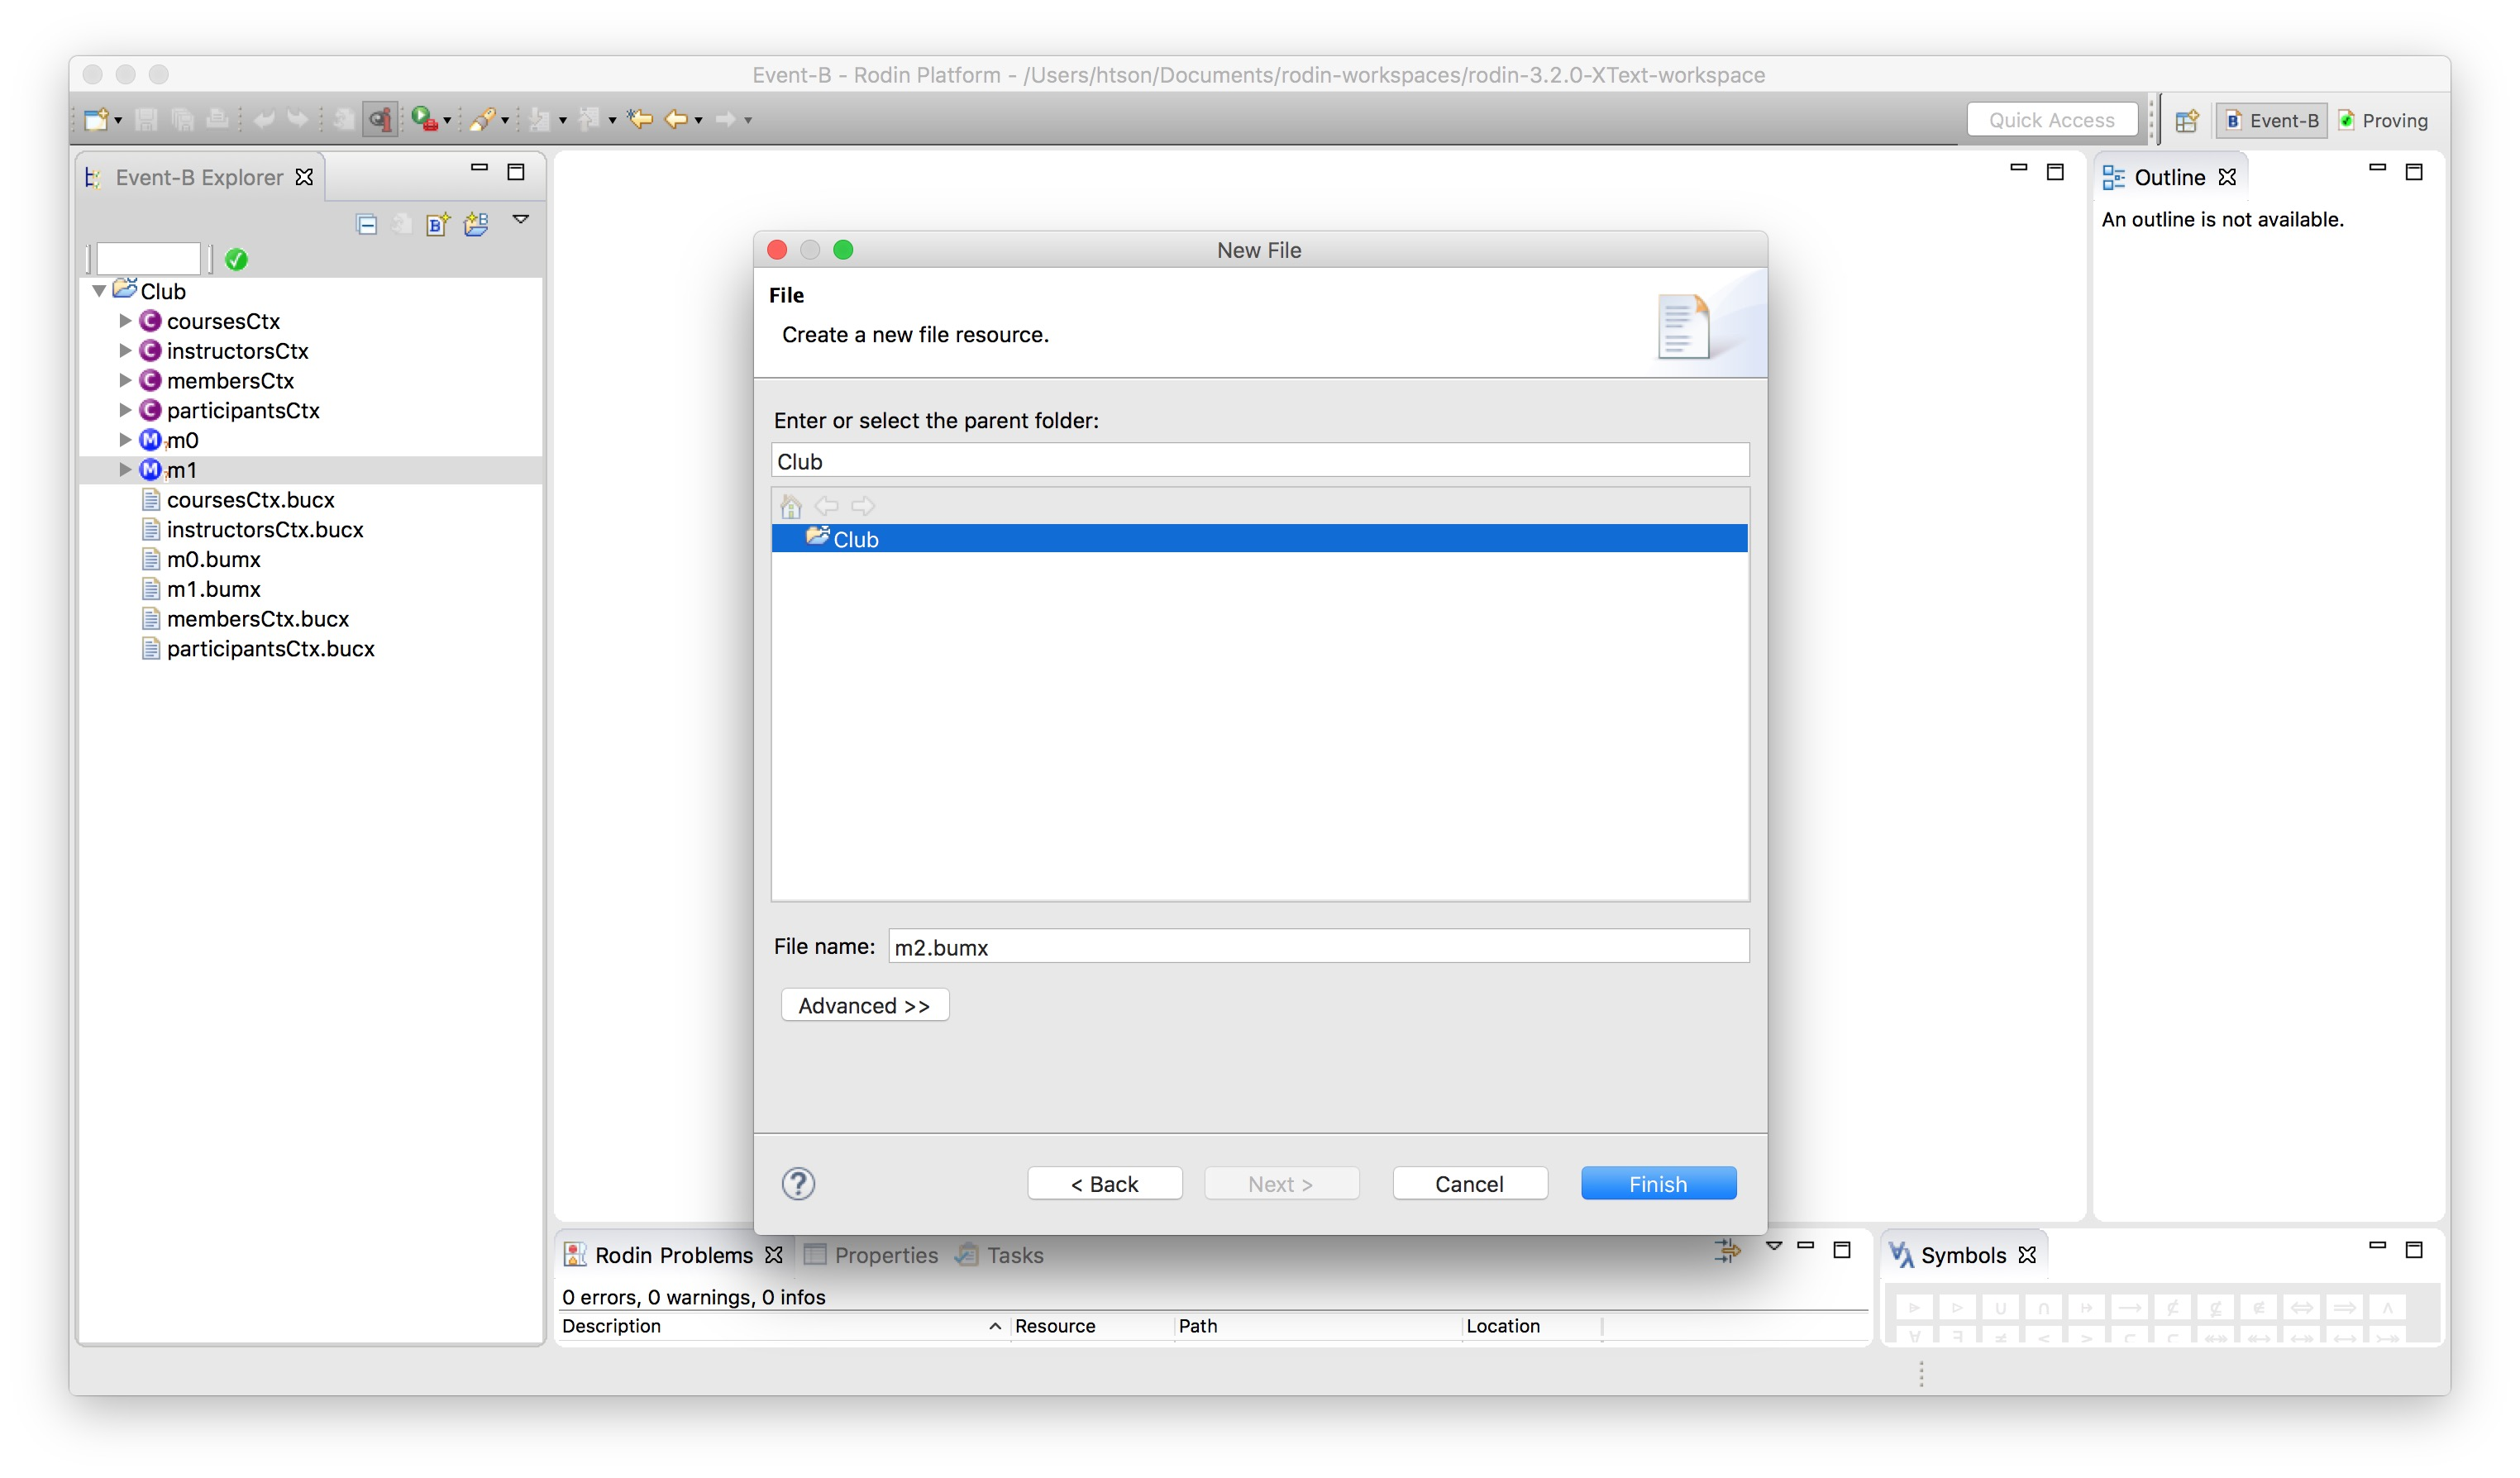
\includegraphics[width=512]{figures/CreateM2}
    \else
    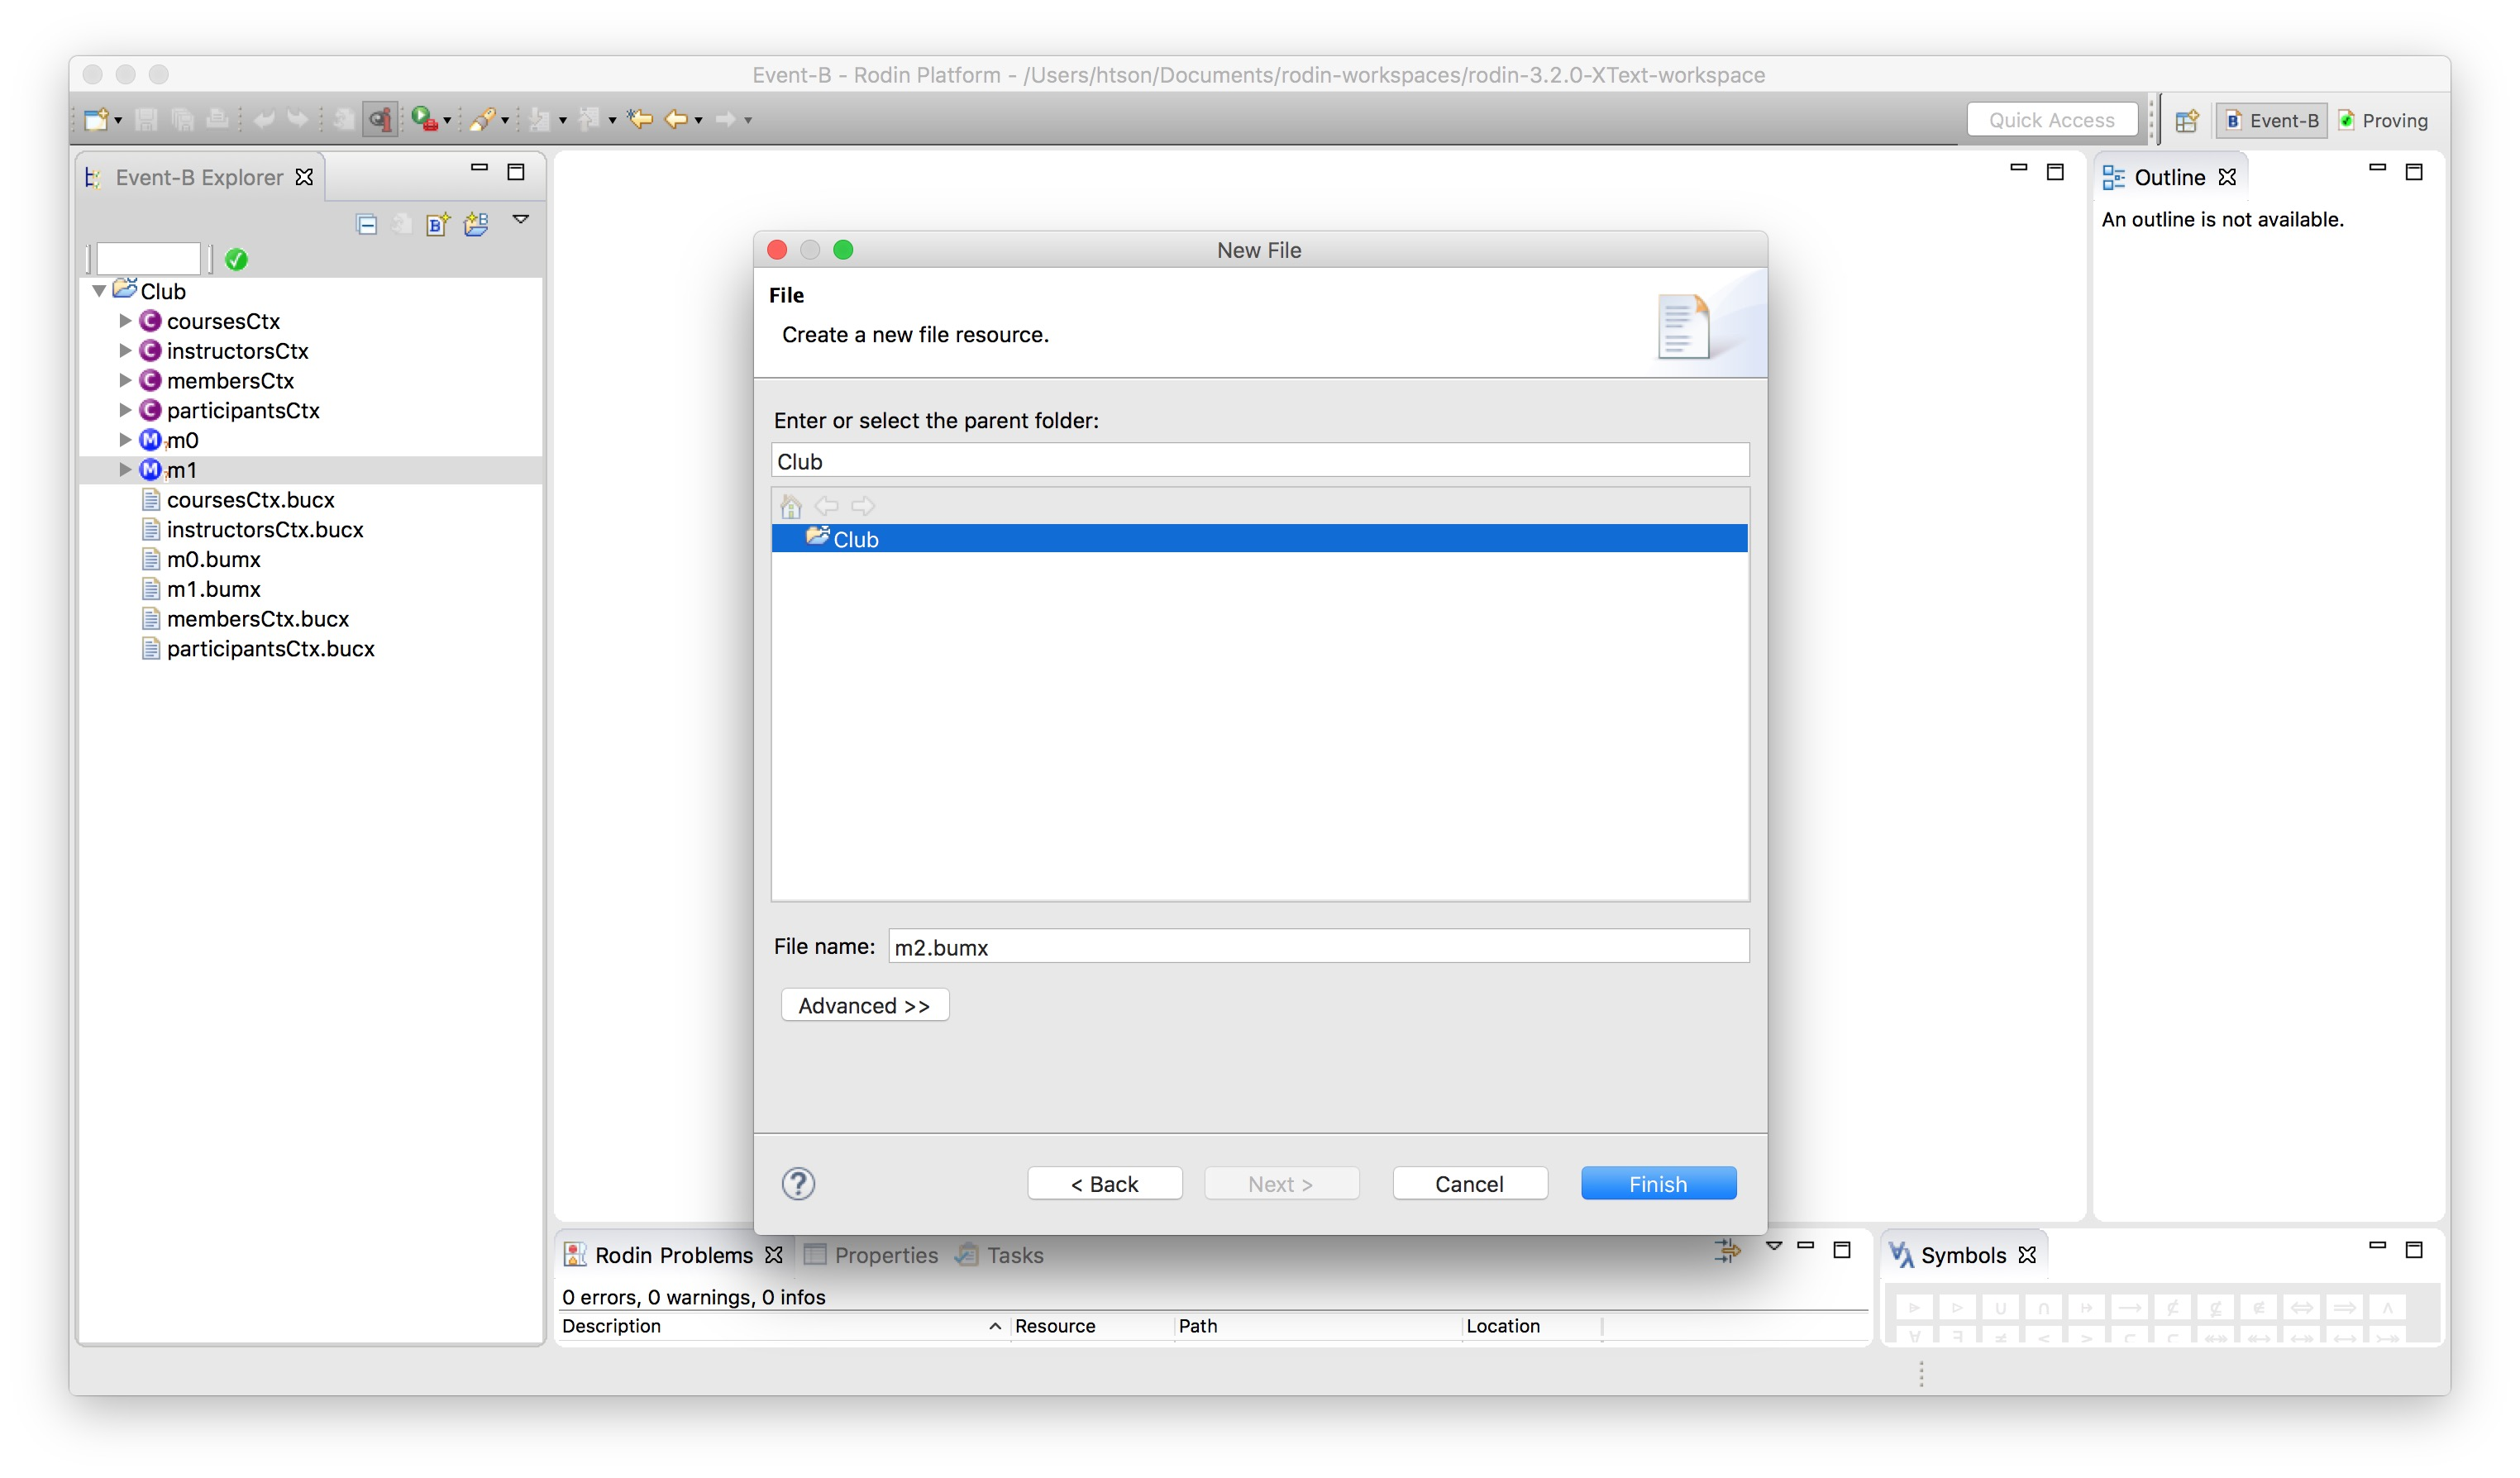
\includegraphics[width=0.9\textwidth]{figures/CreateM2}
    \fi
    \caption{Create m2.bumx}
    \label{fig:CreateM2}
  \end{figure}

\item[Step 2. Set the content of m2.bumx] \textbf{Set the content of ``m2.bumx'' as follows}.
  \begin{center}
    \begin{Bcode}
      \ifplastex
      \Bmachine{} m2\\
      \Brefines{} m1\\
      \Bsees{} instructorsCtx participantsCtx\\
      \Bvariables{} atnds\\
      \Binvariants\\
      @inv2_1: "atnds ∈ CRS ⇸ ℙ(PRTCPT)"\\
      @inv2_2: "crs = dom(atnds)"\\
      @inv2_3: "∀c·c ∈ crs ⇒ prtcpts[\{c\}] = atnds(c)"\\
      @thm2_1: "finite(atnds)" \Btheorem\\
      \Bvariant{} "card(atnds)"\\
      \Bevents\\
      INITIALISATION\\
      \Bbegin\\
      @act2_1: "atnds ≔ ∅"\\
      \Bend\\
      OpenCourse\\
      \Brefines{} OpenCourses\\
      \Bany{} c \Bwhere\\
      @grd2_1: "c ∉ dom(atnds)"\\
      @grd2_2: "card(atnds) ≠ m" \\
      @thm2_2: "card(crs) ≠ m" theorem\\
      \Bwith\\
      @crs': "crs' = crs ∪ \{c\}"\\
      \Bthen\\
      @act2_1: "atnds(c) ≔ ∅"\\
      \Bend\\
      CloseCourse \Bconvergent\\
      \Brefines{} CloseCourses\\
      \Bany{} c \Bwhere\\
      @grd2_1: "c ∈ dom(atnds)"\\
      \Bwith\\
      @cs: "cs = \{c\}"\\
      \Bthen\\
      @act1_2: "atnds ≔\{c\} ⩤ atnds"\\
      \Bend\\
      Register \Bconvergent\\
      \Brefines{} Register\\
      \Bany{} p c \Bwhere\\
      @grd2_1: "p ∈ PRTCPT"\\
      @grd2_2: "p ≠ instrs(c)"\\
      @grd2_3: "c ∈ dom(atnds)"\\
      @grd2_4: "p ∉ atnds(c)"\\
      @thm2_3: "atnds(c) = prtcpts[\{c\}]" theorem\\
      \Bthen\\
      @act2_1: "atnds(c) ≔ atnds(c) ∪ \{p\}"\\
      \Bend\\
      \Bend
      \else
      \Bmachine{} m2\\
      \Brefines{} m1\\
      \Bsees{} instructorsCtx participantsCtx\\
      \Bvariables{} atnds\\
      \Binvariants\\
      \Btab @inv2_1: "\(atnds \in CRS \pfun \pow(PRTCPT)\)"\\
      \Btab @inv2_2: "\(crs = \dom(atnds)\)"\\
      \Btab @inv2_3: "\(\forall c \qdot c \in crs \limp prtcpts[\{c\}] = atnds(c)\)"\\
      \Btab @thm2_1: "\(\finite(atnds)\)" \Btheorem\\
      \Bvariant{} "\(\card(atnds)\)"\\
      \Bevents\\
      \Btab INITIALISATION\\
      \Btab \Bbegin\\
      \Btab \Btab @act2_1: "\(atnds \bcmeq \emptyset\)"\\
      \Btab \Bend\\
      \Btab OpenCourse\\
      \Btab \Brefines{} OpenCourses\\
      \Btab \Bany{} c \Bwhere\\
      \Btab \Btab @grd2_1: "\(c \notin \dom(atnds)\)"\\
      \Btab \Btab @grd2_2: "\(\card(atnds) \neq m\)" \\
      \Btab \Btab @thm2_2: "\(\card(crs) \neq m\)" \Btheorem\\
      \Btab \Bwith\\
      \Btab \Btab @crs': "\(crs' = crs \bunion \{c\}\)"\\
      \Btab \Bthen\\
      \Btab \Btab @act2_1: "\(atnds(c) \bcmeq \emptyset\)"\\
      \Btab \Bend\\
      \Btab CloseCourse \Bconvergent\\
      \Btab \Brefines{} CloseCourses\\
      \Btab \Bany{} c \Bwhere\\
      \Btab \Btab @grd2_1: "\(c \in \dom(atnds)\)"\\
      \Btab \Bwith\\
      \Btab \Btab @cs: "\(cs = \{c\}\)"\\
      \Btab \Bthen\\
      \Btab \Btab @act1_2: "\(atnds \bcmeq \{c\} \domsub atnds\)"\\
      \Btab \Bend\\
      \Btab  Register \Bconvergent\\
      \Btab \Brefines{} Register\\
      \Btab \Bany{} p c \Bwhere\\
      \Btab \Btab @grd2_1: "\(p \in PRTCPT\)"\\
      \Btab \Btab @grd2_2: "\(p \neq instrs(c)\)"\\
      \Btab \Btab @grd2_3: "\(c \in \dom(atnds)\)"\\
      \Btab \Btab @grd2_4: "\(p \notin atnds(c)\)"\\
      \Btab \Btab @thm2_3: "\(atnds(c) = prtcpts[\{c\}]\)" theorem\\
      \Btab \Bthen\\
      \Btab \Btab @act2_1: "\(atnds(c) \bcmeq atnds(c) ∪ \{p\}\)"\\
      \Btab \Bend\\
      \Bend
      \fi
    \end{Bcode}
  \end{center}

\item[Step 3. Auto-format the code] \textbf{Automatically format the content of ``m2.bumx''} by using short-cut (e.g., on Mac OS: Cmd+Shift+F).

\item[Step 4. Save the file] \textbf{Save the file ``m2.bumx''}.
\end{description}
\textbf{Conclusion} By now, the XMachine ``m2.bucx'' and the corresponding Rodin Machine ``m2'' should be visible in the Event-B Explorer (see Figure~\ref{fig:M2}.
  \begin{figure}[!htbp]
    \centering
    \ifplastex
    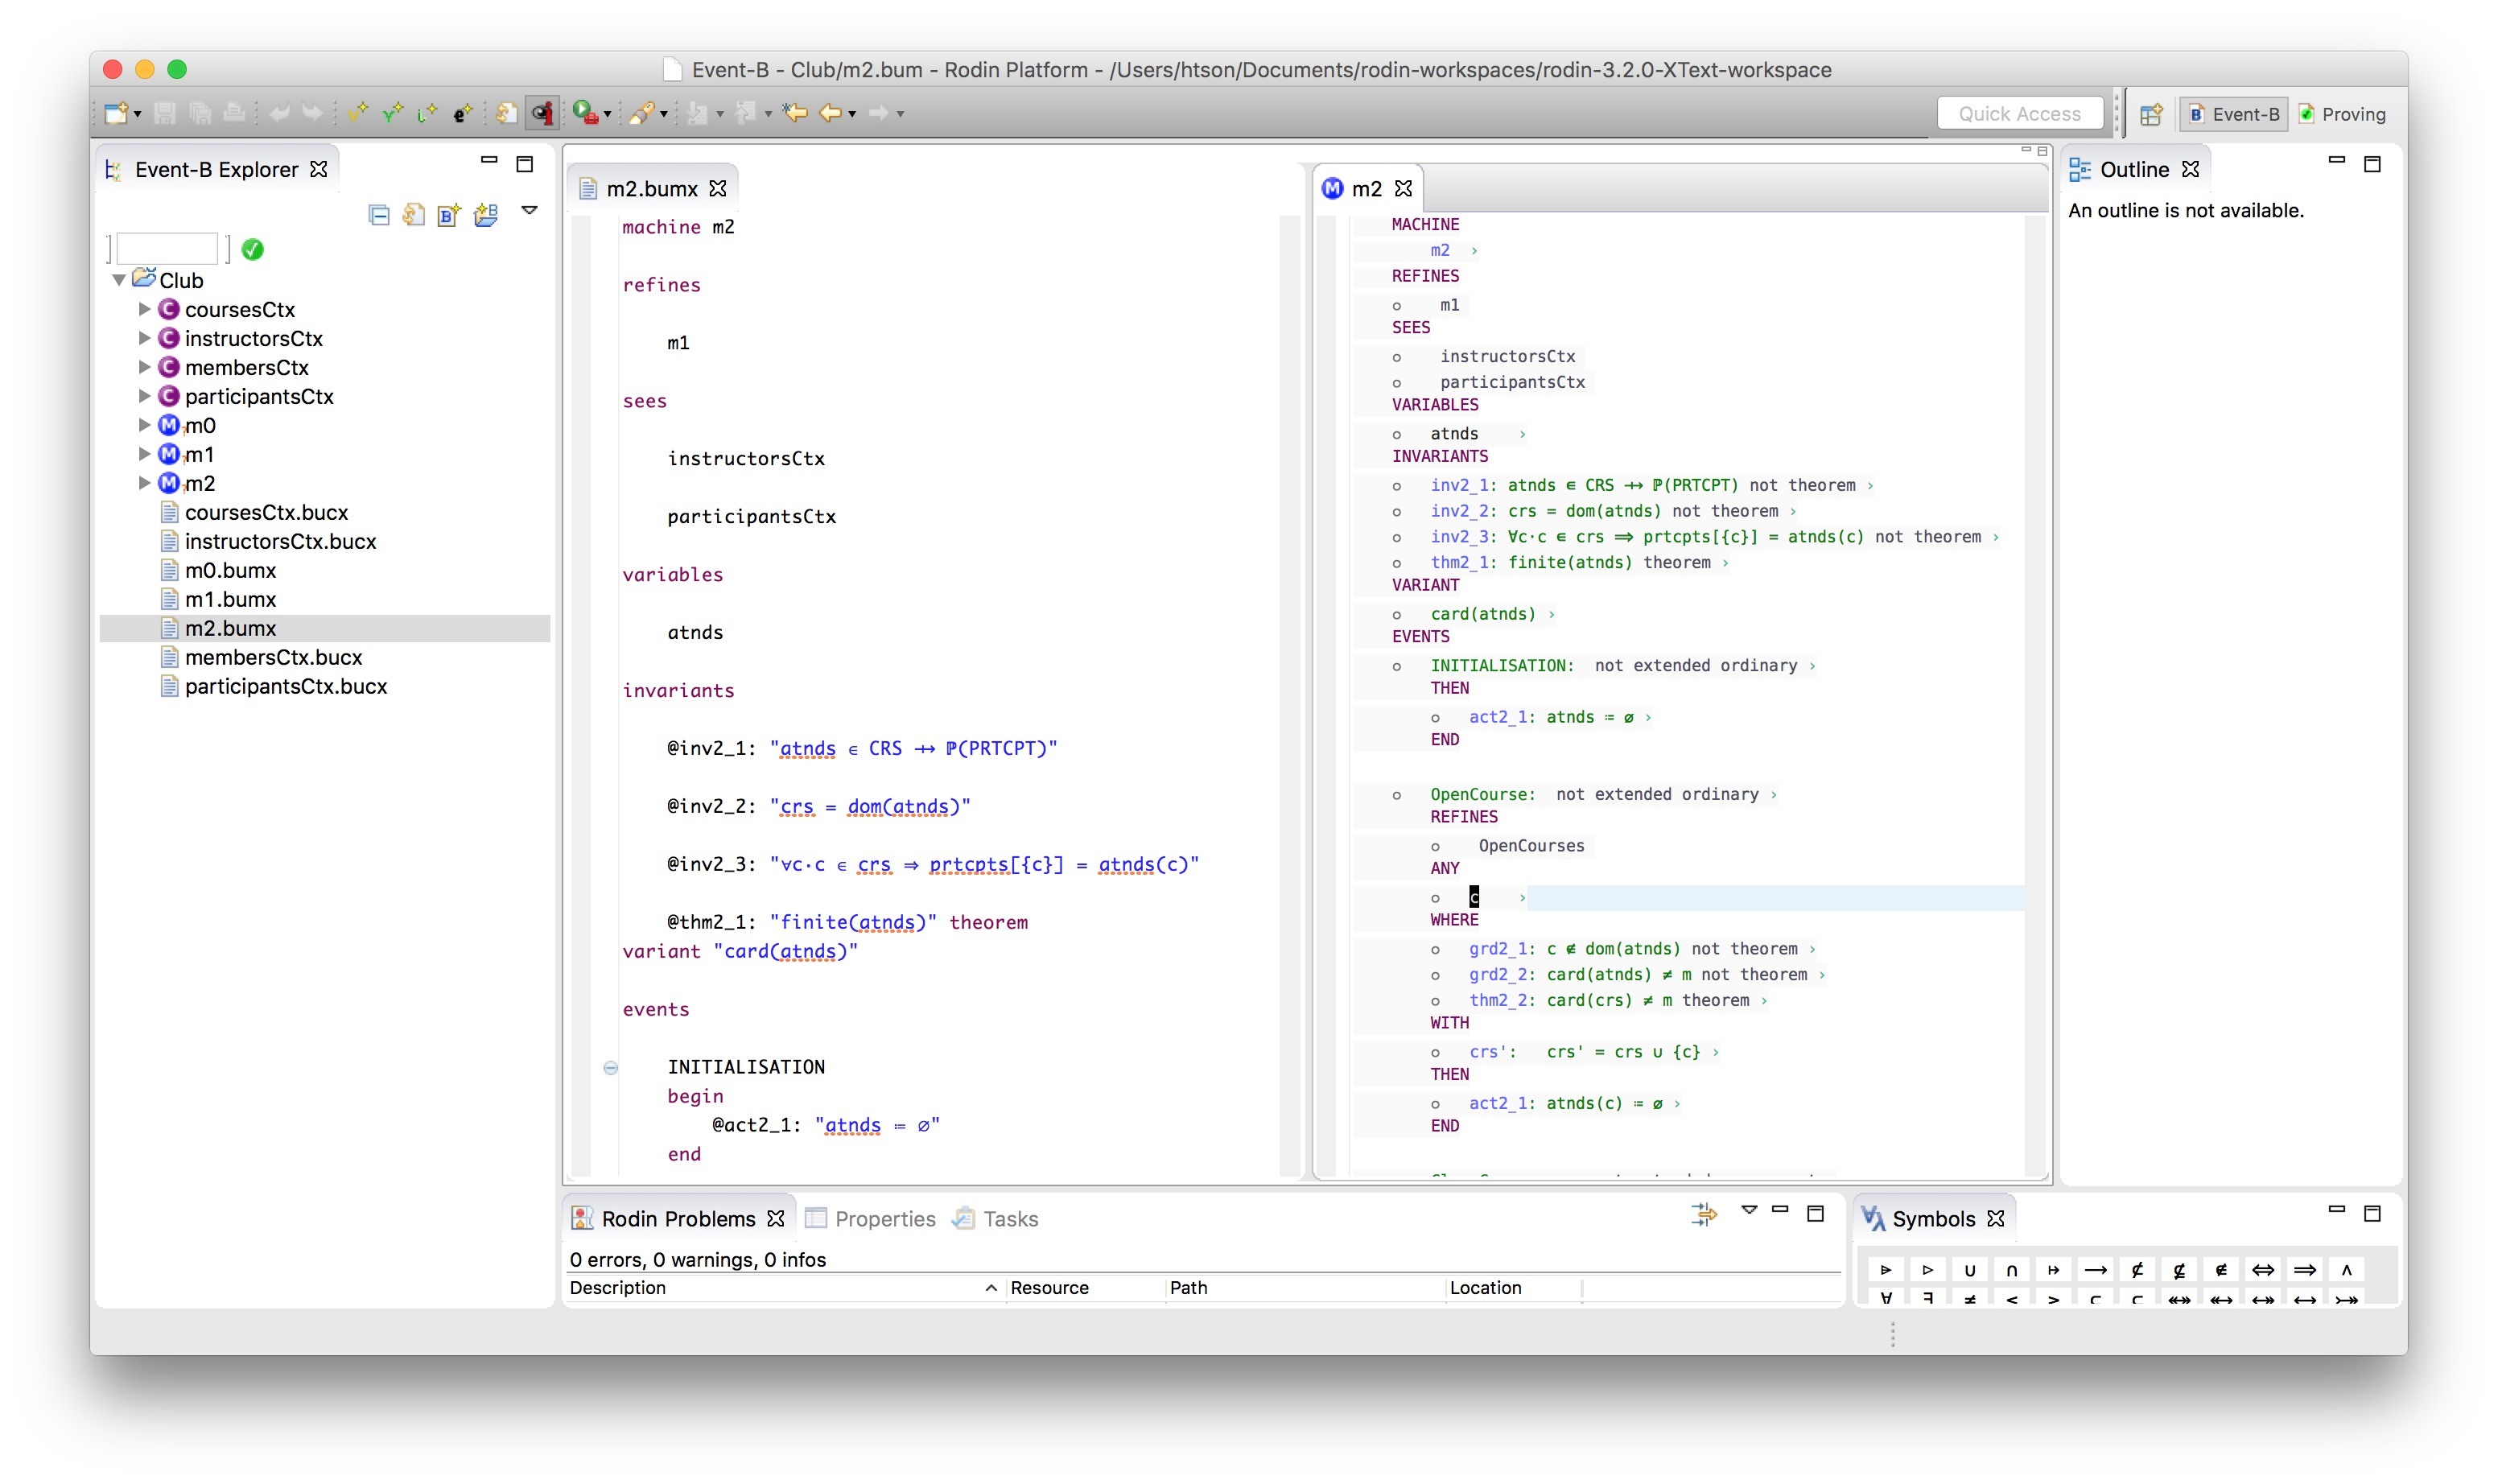
\includegraphics[width=512]{figures/M2}
    \else
    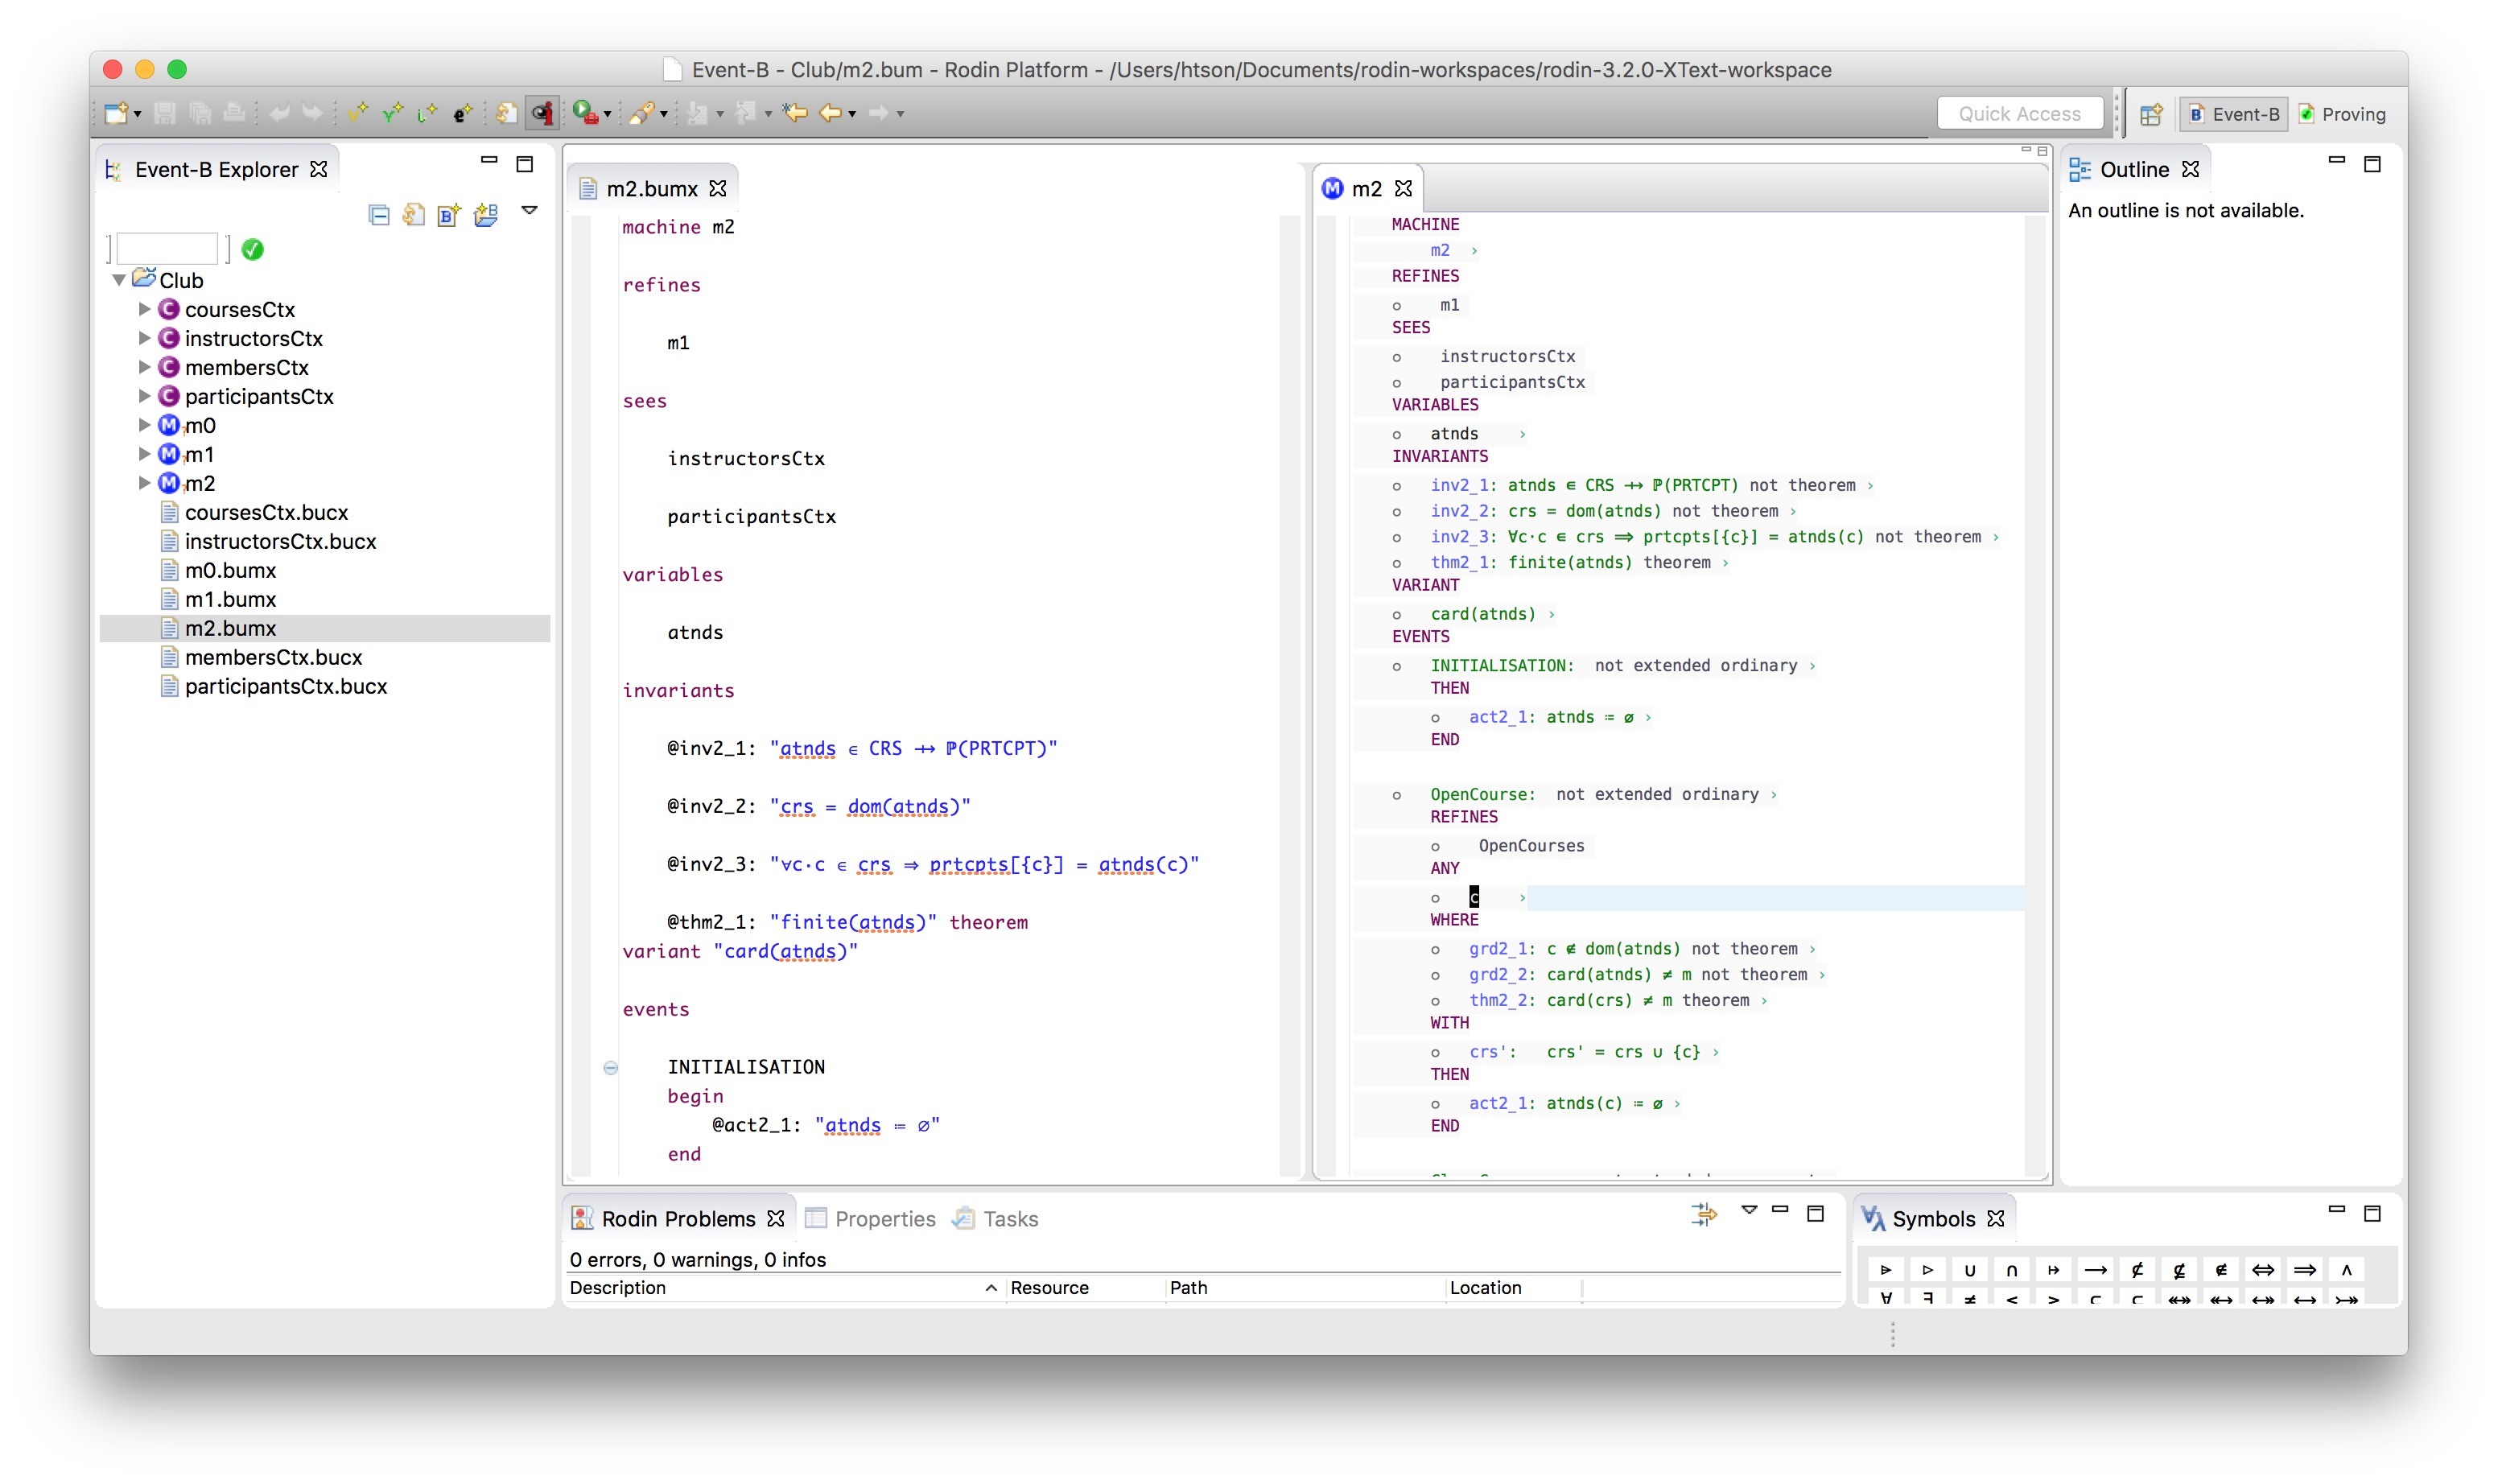
\includegraphics[width=0.9\textwidth]{figures/M2}
    \fi
    \caption{XMachine m2.bumx}
    \label{fig:M2}
  \end{figure}

\subsection{Advanced Tutorial}
\label{sec:advanced-tutorial}

This tutorial provides a step-by-step walk-through working with \emph{machine inclusion} using XEvent-B. Following the same steps as in Section~\ref{sec:basic-tutorial} to create machines and contexts, we can create a machine that can include other machines and can update the included machines variables via \emph{event synchronisation}.

We illustrate the application of machine inclusion using XEvent-B by modelling a small example of ``controlling cars on a bridge'', which is based on Chapter 2 of ``\emph{Modeling in Event-B: System and Software Engineering}'' book.

\subsubsection{Task 1. Create the reusable model}
\textbf{Introduction} The purpose of this task is to create the model that will be reused by other models using machine inclusion.
\begin{description}
\item[Step 1. Create a new Project (Sensor) with XMachine m0\_SNSR.bumx] 

Following the same steps as 
\ifplastex
in tasks 2 and 4 in Section~\ref{sec:basic-tutorial} for creating project and machines.
\else
in Sections~\ref{CreateProject} and~\ref{CreateMachine} for creating project and machines.
\fi

\item[Step 2. Set the content of m0\_SNSR.bumx] \textbf{Set the content of ``m0\_SNSR.bumx'' as follows}.
\begin{center}
	\begin{Bcode}
		\ifplastex
		\Bmachine{} m0_SNSR\\
		\Bvariables{} SNSR\\
		\Binvariants\\
		@thm0_1: "SNSR ∈ BOOL" \Btheorem\\
		\Bevents\\
		INITIALISATION\\
		\Bbegin\\
		@act1: "SNSR ≔ FALSE"\\
		\Bend\\
		SNSR_on\\
		\Bwhen\\
		@grd1: "SNSR = FALSE"\\
		\Bthen\\
		@act1: "SNSR ≔ TRUE"\\
		\Bend\\
	    SNSR_off\\
	    \Bwhen\\
	    @grd1: "SNSR = TRUE"\\
	    \Bthen\\
	    @act1: "SNSR ≔ FALSE"\\
	    \Bend\\
		\Bend
		\else
		\Bmachine{} m0_SNSR\\
		\Bvariables{} SNSR\\
		\Binvariants\\
		\Btab @thm0_1: "\(SNSR \in BOOL\)" \Btheorem\\
		\Bevents\\
		\Btab INITIALISATION\\
		\Btab \Bbegin\\
		\Btab \Btab @act1: "\(SNSR \bcmeq FALSE\)"\\
		\Btab \Bend\\
		\Btab SNSR_on\\
		\Btab \Bwhen\\
		\Btab \Btab @grd1: "\(SNSR = FALSE\)"\\
		\Btab \Bthen\\
		\Btab \Btab @act1: "\(SNSR \bcmeq TRUE\)"\\
		\Btab \Bend\\
		\Btab SNSR_off\\
		\Btab \Bwhen\\
		\Btab \Btab @grd1: "\(SNSR = TRUE\)"\\
		\Btab \Bthen\\
		\Btab \Btab @act1: "\(SNSR \bcmeq FALSE\)"\\
		\Btab \Bend\\
		\Bend
		\fi
	\end{Bcode}
\end{center}

\item[Step 3. Auto-format and Save the file ``m0\_SNSR.bumx''] 
\end{description}

\textbf{Conclusion} By now, the XMachine ``m0\_SNSR.bumx'' and the corresponding Rodin Machine ``m0\_SNSR'' should be visible in the Event-B Explorer.

\subsubsection{Task 2. Model the abstract level of cars on a bridge}
\textbf{Introduction} The purpose of this task is to create the abstract model of the ``cars on a bridge'' example. At this level, we have not applied machine inclusion, but it is possible to apply machine inclusion right from the abstract level. 
\begin{description}
	\item[Step 1. Create the Context Car\_c0\_limit.bucx in a new project Car] 
	Following the same steps as 
	\ifplastex
	in task 3 of Section~\ref{sec:basic-tutorial} for creating a simple context.  
	\else
	in Section~\ref{Sec:SimpleContext} for creating a simple context.
	\fi
	\textbf{Set the content of ``Car\_c0\_limit.bucx'' as follows and save the file}.
	  
	  \begin{center}
		\begin{Bcode}
			\ifplastex
			\Bcontext{} Car\_c0_limit\\
			\Bconstants{} D\\
			\Baxioms\\
			@axm1: "D ∈ ℕ1"\\
			\Bend
			\else
			\Bcontext{} Car_c0_limit\\
			\Bconstants{} D\\
			\Baxioms\\
			\Btab @axm1: "\(D \in \nat1\)"\\
			\Bend
			\fi
		\end{Bcode}
	\end{center}
	\item[Step 2. Create the Machine Car\_m0\_cars.bumx]\textbf{Set the content of ``Car\_m0\_cars.bumx'' as follows and save the file}.

	\begin{center}
		\begin{Bcode}
			\ifplastex
			\Bmachine{} Car\_m0_cars\\
			\Bsees{} Car\_c0_limit\\
			\Bvariables{} A B C\\
			\Binvariants\\
			@inv0_1: "A ∈ ℕ"\\
			@inv0_2: "B ∈ ℕ"\\
			@inv0_3: "C ∈ ℕ"\\
			@inv0_4: "A = 0 ∨ C = 0"\\
			@inv0_5: "A + B + C ≤ D"\\
			@thm0_1: "B ≤ D" \Btheorem\\
			\Bevents\\
			INITIALISATION\\
			\Bbegin\\
			@act1: "A ≔ 0"\\
			@act2: "B ≔ 0"\\
			@act3: "C ≔ 0"\\
			\Bend\\
			ML_out\\
			\Bwhen\\
			@grd1: "C = 0"\\
			@grd2: "A + B ≠ D"\\
			\Bthen\\
			@act1: "A ≔ A + 1"\\
			\Bend\\
			ML_in\\
			\Bwhen\\
			@grd1: "C ≠ 0"\\
			\Bthen\\
			@act1: "C ≔ C − 1"\\
			\Bend\\
			IL_in\\
			\Bwhen\\
			@grd1: "A ≠ 0"\\
			\Bthen\\
			@act1: "A ≔ A − 1"\\
			@act2: "B ≔ B + 1"\\
			\Bend\\
			IL_out\\
			\Bwhen\\
			@grd1: "B ≠ 0"\\
			@grd2: "A = 0"\\
			\Bthen\\
			@act1: "B ≔ B − 1"\\
			@act2: "C ≔ C + 1"\\
			\Bend\\
			\Bend
			\else
			\Bmachine{} Car\_m0_cars\\
			\Bsees{} Car\_c0_limit\\
			\Bvariables{} A B C\\
			\Binvariants\\
			\Btab @inv0_1: "\(A \in \nat\)"\\
			\Btab @inv0_2: "\(B \in \nat"\)\\
			\Btab @inv0_3: "\(C \in \nat\)"\\
			\Btab @inv0_4: "\(A = 0 \vee C = 0\)"\\
			\Btab @inv0_5: "\(A + B + C \leq D\)"\\
			\Btab @thm0_1: "\(B \leq D\)" \Btheorem\\
			\Bevents\\
			\Btab INITIALISATION\\
			\Btab \Bbegin\\
			\Btab \Btab @act1: "\(A \bcmeq 0\)"\\
			\Btab \Btab @act2: "\(B \bcmeq 0\)"\\
			\Btab \Btab @act3: "\(C \bcmeq 0\)"\\
			\Btab \Bend\\
			\Btab ML_out\\
			\Btab \Bwhen\\
			\Btab \Btab @grd1: "\(C = 0\)"\\
			\Btab \Btab @grd2: "\(A + B \neq D\)"\\
			\Btab \Bthen\\
			\Btab \Btab @act1: "\(A \bcmeq A + 1\)"\\
			\Btab \Bend\\
			\Btab ML_in\\
			\Btab \Bwhen\\
			\Btab \Btab @grd1: "\(C \neq 0\)"\\
			\Btab \Bthen\\
			\Btab \Btab @act1: "\(C \bcmeq C - 1\)"\\
			\Btab \Bend\\
			\Btab IL_in\\
			\Btab \Bwhen\\
			\Btab \Btab @grd1: "\(A \neq 0\)"\\
			\Btab \Bthen\\
			\Btab \Btab @act1: "\(A \bcmeq A - 1\)"\\
			\Btab \Btab @act2: "\(B \bcmeq B + 1\)"\\
			\Btab \Bend\\
			\Btab IL_out\\
			\Btab \Bwhen\\
			\Btab \Btab @grd1: "\(B \neq 0\)"\\
			\Btab \Btab @grd2: "\(A = 0\)"\\
			\Btab \Bthen\\
			\Btab \Btab @act1: "\(B \bcmeq B - 1\)"\\
			\Btab \Btab @act2: "\(C \bcmeq C + 1\)"\\
			\Btab \Bend\\
			\Bend
			\fi
		\end{Bcode}
	\end{center}
	
\end{description}
\textbf{Conclusion} Saving the XContext and XMachine files will generate the corresponding Rodin files. In the ``Car'' you have the context ``Car\_c0\_limit'' and the machine ``Car\_m0\_cars''. Ideally the reusable models should be in a different project, that is why we added the reusable model in a different project ``Sensor''.

\subsubsection{Task 3. Model an XMachine using machine inclusion}
\textbf{Introduction} In this task we define the XMachine ``Car\_m1\_SNSR.bumx'' which is a refinement of the machine ``Car\_m0\_cars'' and includes two instances of ``m0\_SNSR''. The keywords in red  are \textbf{not} part of the standard Event-B syntax, they correspond to machine inclusion and event synchronisation. 

\begin{description}
	\item[Step 1. Create the file ``Car\_m1\_SNSR.bumx''] \textbf{Set its contents as follows.}
	
		\begin{center}
		\begin{Bcode}
			\ifplastex
			\Bmachine{} Car_m1_SNSR\\
			\textcolor{red}{\textbf{includes}} Sensor.m0_SNSR \textcolor{red}{\textbf{as}} IL_out ML_out\\
			\Brefines{} Car_m0_cars\\
			\Bsees{} Car_c0_limit\\
			\Bvariables{} A B C\\
			\Binvariants\\
			@inv1_1: "IL_out_SNSR = TRUE ⇒ B ≠ 0"\\
			\Bevents\\
			INITIALISATION \Bextended\\
			\textcolor{red}{\textbf{synchronises}} IL_out.INITIALISATION\\
			\textcolor{red}{\textbf{synchronises}} ML_out.INITIALISATION\\
			\Brefines{} INITIALISATION\\
			\Bend\\
			ML_out \Bextended\\
			\textcolor{red}{\textbf{synchronises}} ML_out.SNSR_off\\
			\Brefines{} ML_out\\
			\Bend\\
			ML_in \Bextended\\
			\Brefines{} ML_in\\
			\Bend\\
			IL_in \Bextended\\
			\Brefines{} IL_in\\
			\Bwhen\\
			@inv0_2−copy: "B ∈ ℕ" \Btheorem\\
			\Bend\\
			IL_out\\
			\textcolor{red}{\textbf{synchronises}} IL_out.SNSR_off\\
			\Brefines{} IL_out\\
			\Bwhen\\
			@grd2: "A = 0"\\
			\Bthen\\
			@act1: "B ≔ B − 1"\\
			@act2: "C ≔ C + 1"\\
			\Bend\\
			ML_out_ARR\\
			\textcolor{red}{\textbf{synchronises}} ML_out.SNSR_on\\
			\Bend\\
			IL_out_ARR\\
			\textcolor{red}{\textbf{synchronises}} IL_out.SNSR_on\\
			\Bwhen\\
			@grd2: "B ≠ 0"\\
			\Bend\\
			\Bend
			\else
			\Bmachine{} Car_m1_SNSR\\
			\textcolor{red}{includes} Sensor.m0_SNSR \textcolor{red}{as} IL_out ML_out\\
			\Brefines{} Car_m0_cars\\
			\Bsees{} Car_c0_limit\\
			\Bvariables{} A B C\\
			\Binvariants\\
			\Btab @inv1_1: "\("IL_out_SNSR = TRUE \Rightarrow B \neq 0"\)"\\
			\Bevents\\
			\Btab INITIALISATION \Bextended\\
			\Btab \textcolor{red}{synchronises} IL_out.INITIALISATION\\
            \Btab \textcolor{red}{synchronises} ML_out.INITIALISATION\\
            \Btab \Brefines{} INITIALISATION\\
			\Btab \Bend\\
			\Btab ML_out \Bextended\\
			\Btab \textcolor{red}{synchronises} ML_out.SNSR_off\\
			\Btab \Brefines{} ML_out\\
			\Btab \Bend\\
			\Btab ML_in \Bextended\\
			\Btab \Brefines{} ML_in\\
			\Btab \Bend\\
			\Btab IL_in \Bextended\\
			\Btab \Brefines{} IL_in\\
			\Btab \Bwhen\\
			\Btab \Btab @inv0_2−copy: "\(B \in \nat\)" \Btheorem\\
			\Btab \Bend\\
			\Btab IL_out\\
			\Btab \textcolor{red}{synchronises} IL_out.SNSR_off\\
			\Btab \Brefines{} IL_out\\
			\Btab \Bwhen\\
			\Btab \Btab @grd2: "\(A = 0\)"\\
			\Btab \Bthen\\
			\Btab \Btab @act1: "\(B \bcmeq B - 1\)"\\
			\Btab \Btab @act2: "\(C \bcmeq C + 1\)"\\
			\Btab \Bend\\
			\Btab ML_out_ARR\\
			\Btab \textcolor{red}{synchronises} ML_out.SNSR_on\\
			\Btab \Bend\\
			\Btab IL_out_ARR\\
			\Btab \textcolor{red}{synchronises} IL_out.SNSR_on\\
			\Btab \Bwhen\\
			\Btab \Btab @grd2: "\(B \neq 0\)"\\
			\Btab \Bend\\
			\Bend
			\fi
		\end{Bcode}
	\end{center}
	\item[Step 2. Auto-format the file ``Car\_m1\_SNSR.bumx'' and Save it.]
\end{description}
\textbf{Conclusion} After saving the file a standard Event-B machine ``Car\_m1\_SNSR''will be generated. The generated machine (Figure~\ref{fig:FlattenedMachine}) is flattened to include the variables and invariants  of the included machine ``m0\_SNSR'' which are renamed according to the chosen prefixes. In addition to the guards and actions of the synchronised events. The project name must be specified when including a machine (e.g., Sensor.m0\_SNSR), and the project (Sensor) of the included machines must be opened in the same workspace. You can also use content assist to see all available machines in the workspace.

When synchronising an event you can add the prefix of the required machine followed by the synchronised event name (e.g., IL\_out.SNSR\_on where ``IL\_out'' is one of the included machine prefixes and ``SNSR\_on'' is the synchronised event). It is also possible to include more than one machine and synchronise with more than one event. Notice the order of the generated elements in the flattened machine is the included elements from last to first then the source machine elements.

\begin{figure}[!htbp]
	\centering
	\ifplastex
	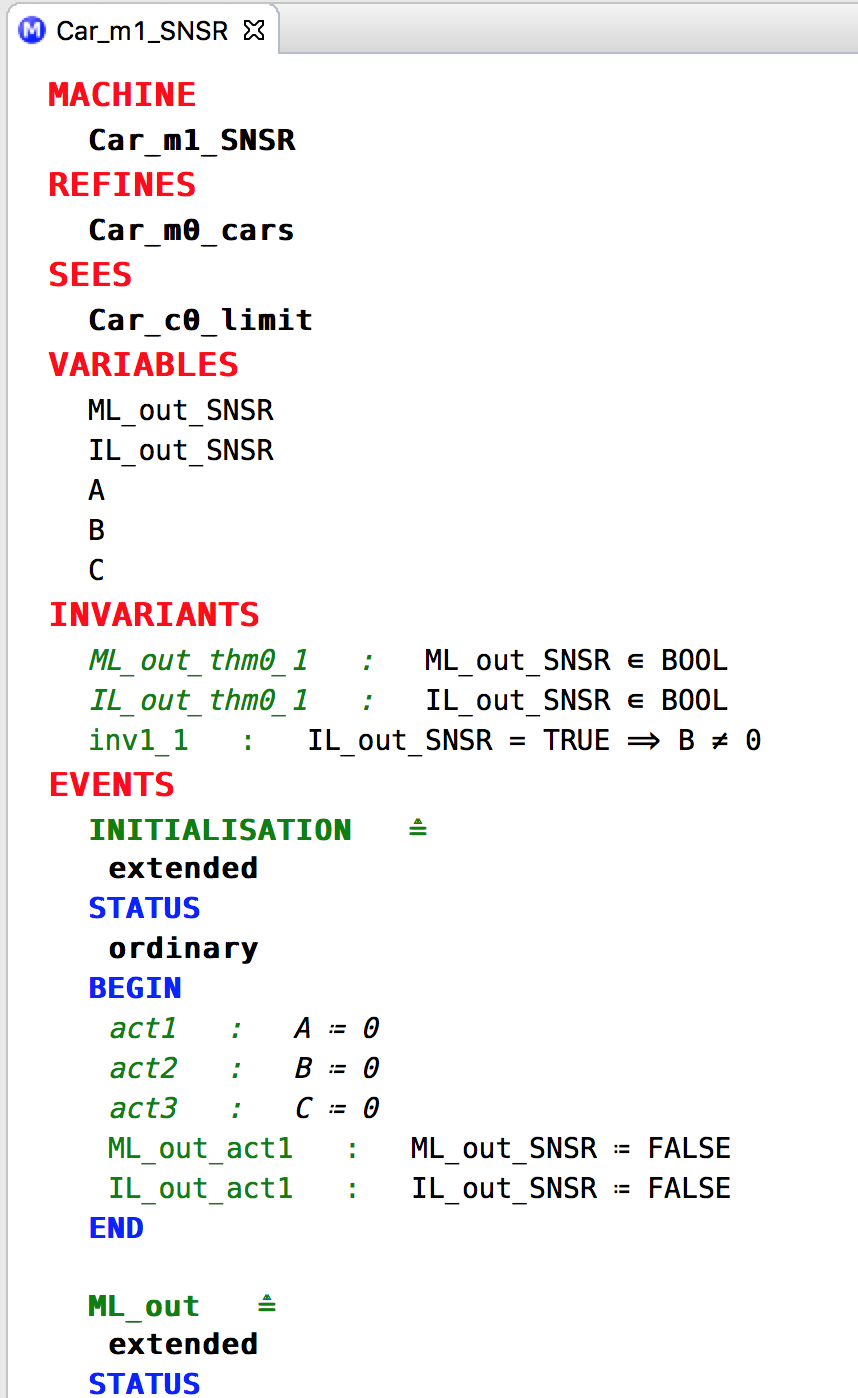
\includegraphics[width=512]{figures/Flattened_var_m1_snsr}
	\else
	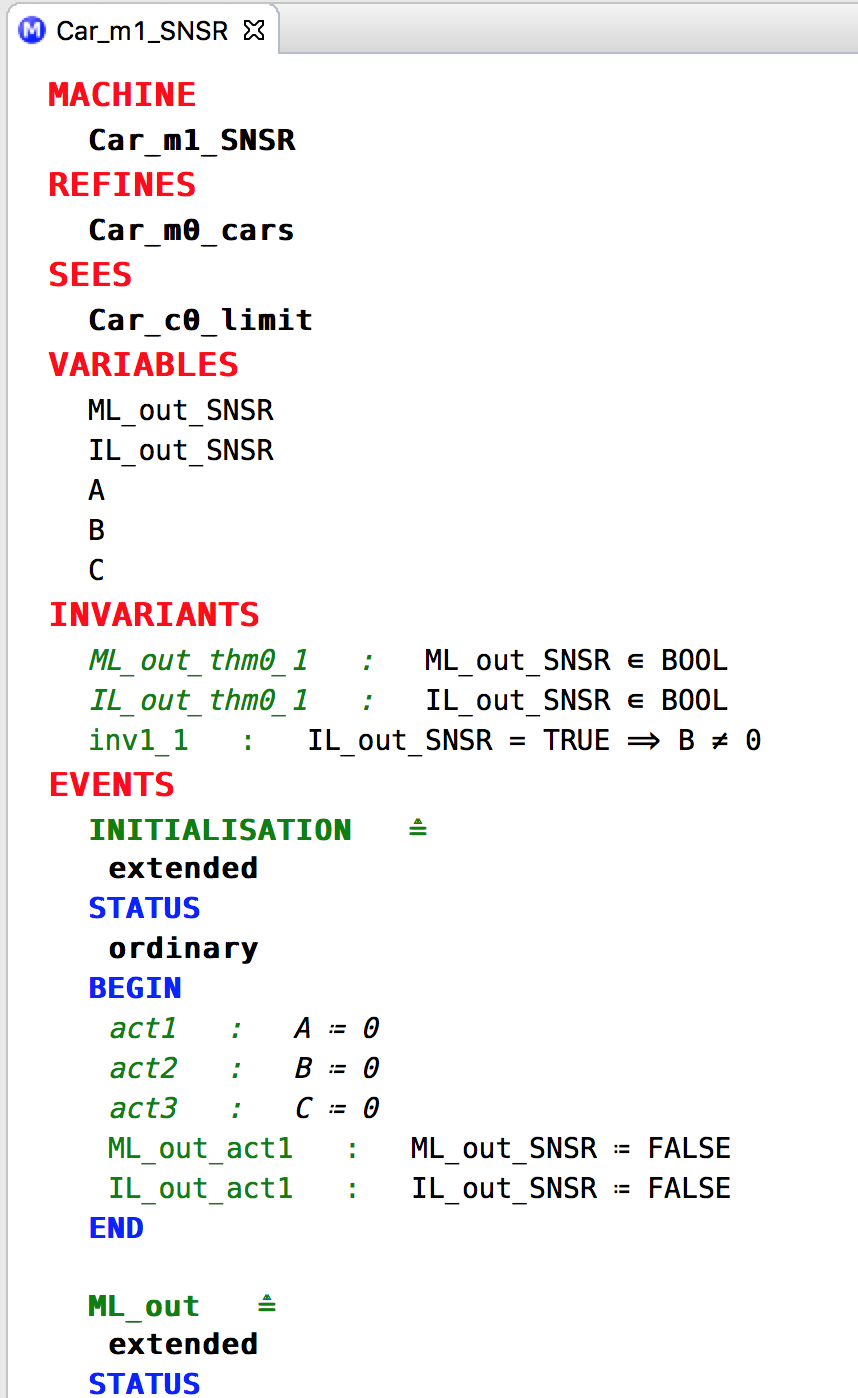
\includegraphics[width=0.9\textwidth]{figures/Flattened_var_m1_snsr}
	\fi
	\caption{Flattened Machine ``Car\_m1\_SNSR''}
	\label{fig:FlattenedMachine}
\end{figure}

% probably here add a figure of the flattened machine to show how variables, inv, gurads are copied and renamed

%%% Local Variables:
%%% mode: latex
%%% TeX-master: "user_manual"
%%% End:


\section{Concepts}
\label{sec:concepts}

\subsection{XText Projects}
\label{sec:xtext-projects}

Each project containing XEvent-B constructs must be set to be XText project.  An XText project has an associated XContext and XMachine builders that can compile XEvent-B source files into Rodin files as they are changed.  The builders can be turn off via the preferences, either workspace-wise or project-wise (see Figure~\ref{fig:XContextPreference}.
\begin{figure}[!htbp]
  \centering
  \ifplastex
  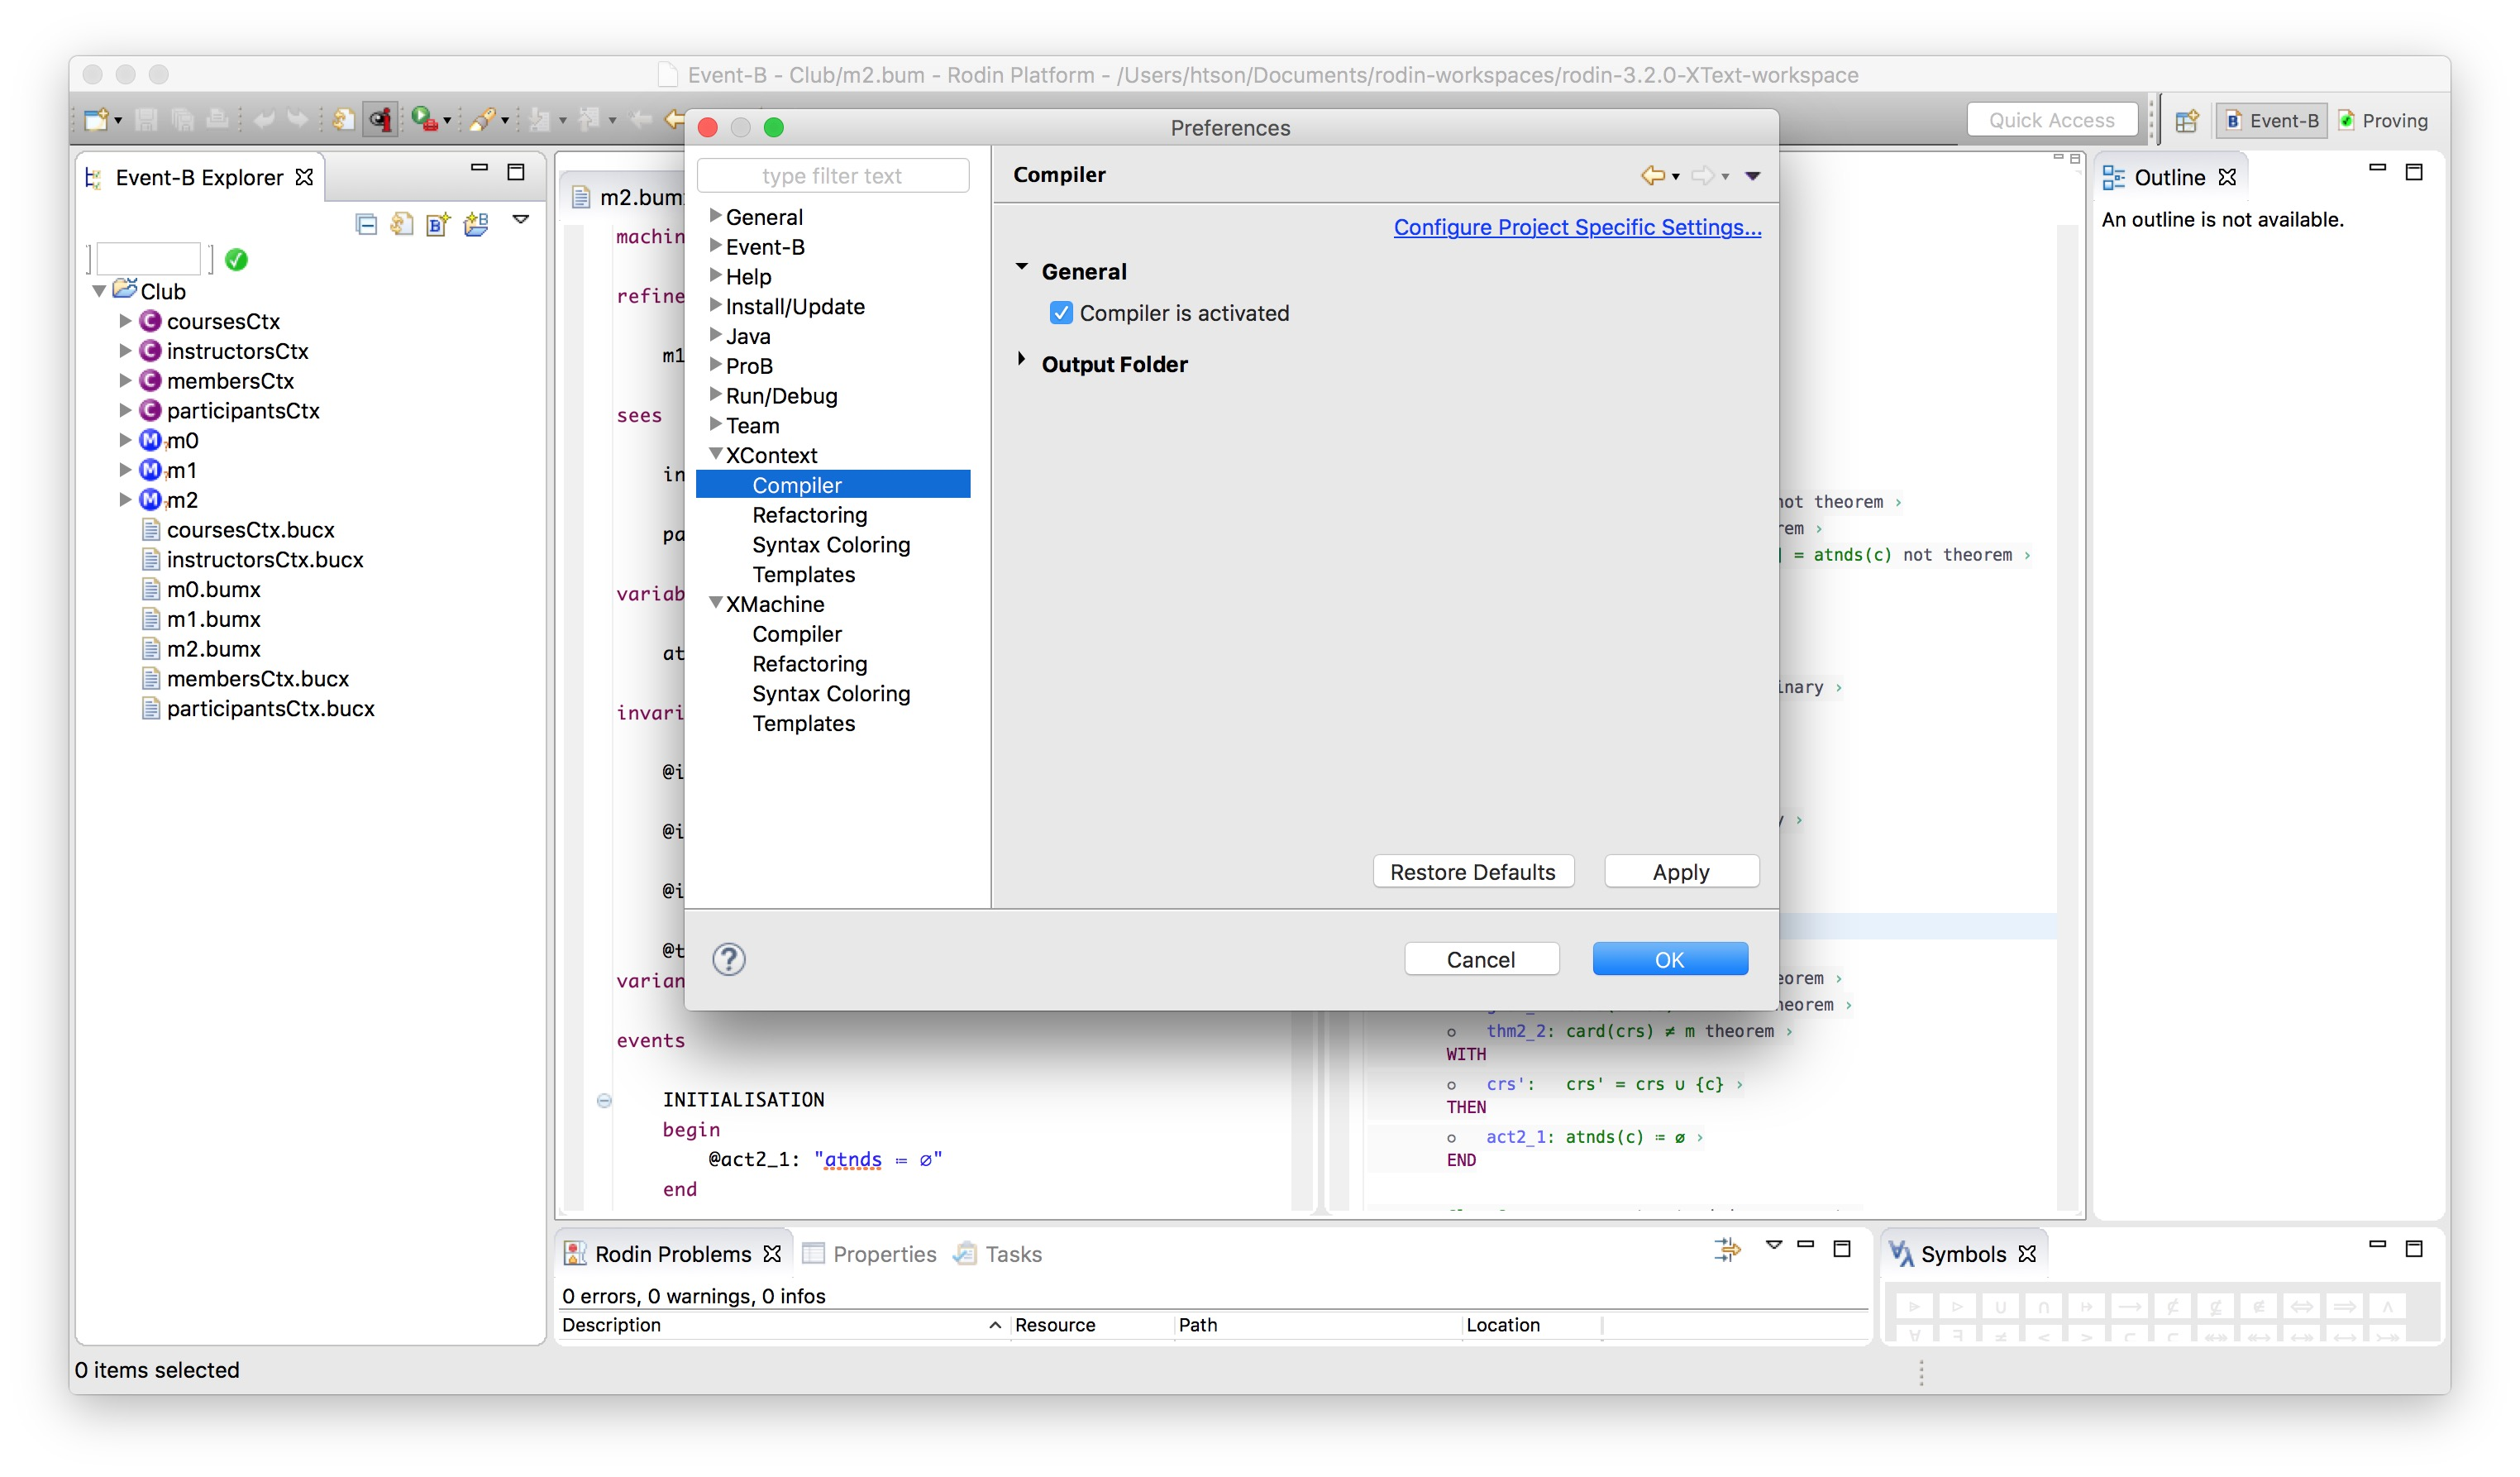
\includegraphics[width=512]{figures/XContextPreference}
  \else
  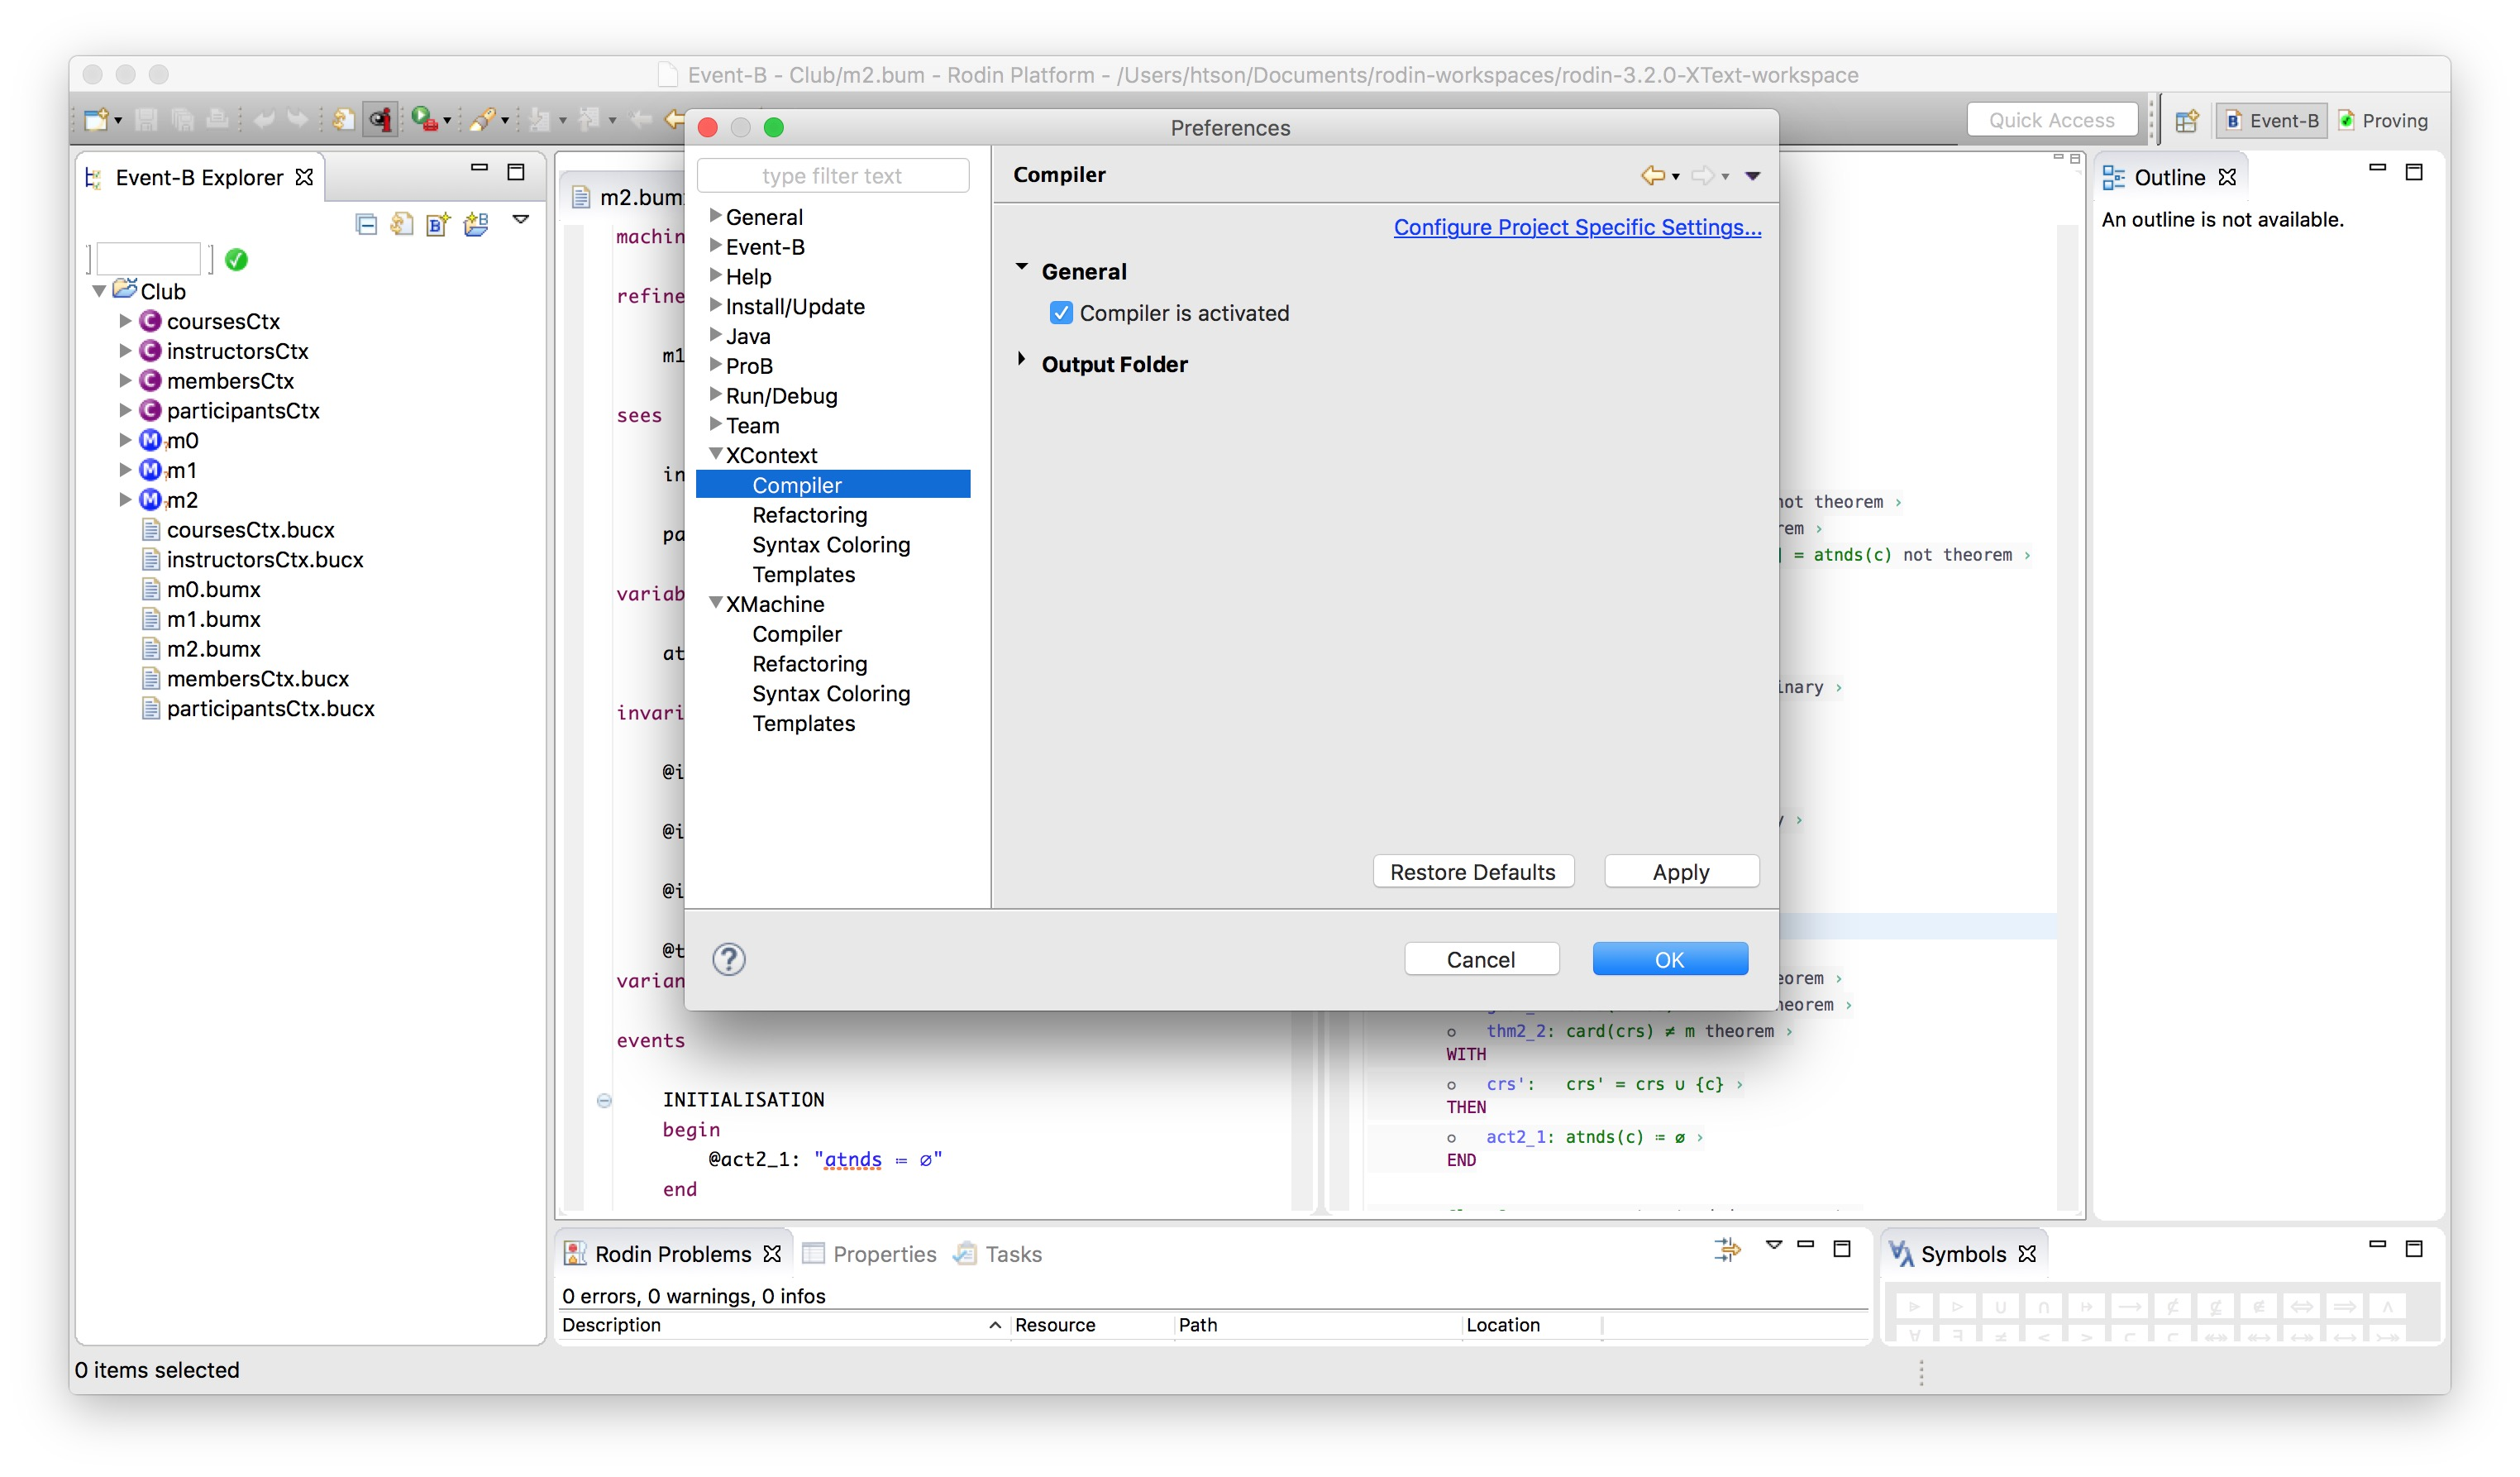
\includegraphics[width=0.9\textwidth]{figures/XContextPreference}
  \fi
  \caption{XContext Preference}
  \label{fig:XContextPreference}
\end{figure}

The XText projects must be organised such that all XEvent-B constructs has the project as the source container.

\subsection{XEvent-B Builders}
\label{sec:xevent-b-builders}
The XEvent-B Builders, i.e., XContext builder and XMachine builder, build XEvent-B constructs, i.e., XContext and XMachine using their own compiler.  If they are enabled, the XEvent-B builders are run everytime an individual XEvent-B file is saved.  Problems detected by the XEvent-B builders are classified as either warnings or errors.  Compile-time errors are always reported as errors by the XEvent-B buiders and in the presence of errors, no new Rodin files are created or updated, i.e., the XEvent-B builders do not produce any new Rodin file content. In the case of machine inclusion and event synchronisation, a flattened machine is generated which includes data from the included machine and the synchronised events, which can be renamed if prefixing is applied.

\subsection{Content Assist}
\label{sec:content-assist}
Content assist are available for typesetting keywords and Event-B mathematical symbols. The short-cut for invoking content assist is \texttt{Ctrl+Space}.  Figure~\ref{fig:KeywordContentAssist} shows an example for content assist with keywords.
\begin{figure}[!htbp]
  \centering
  \ifplastex
  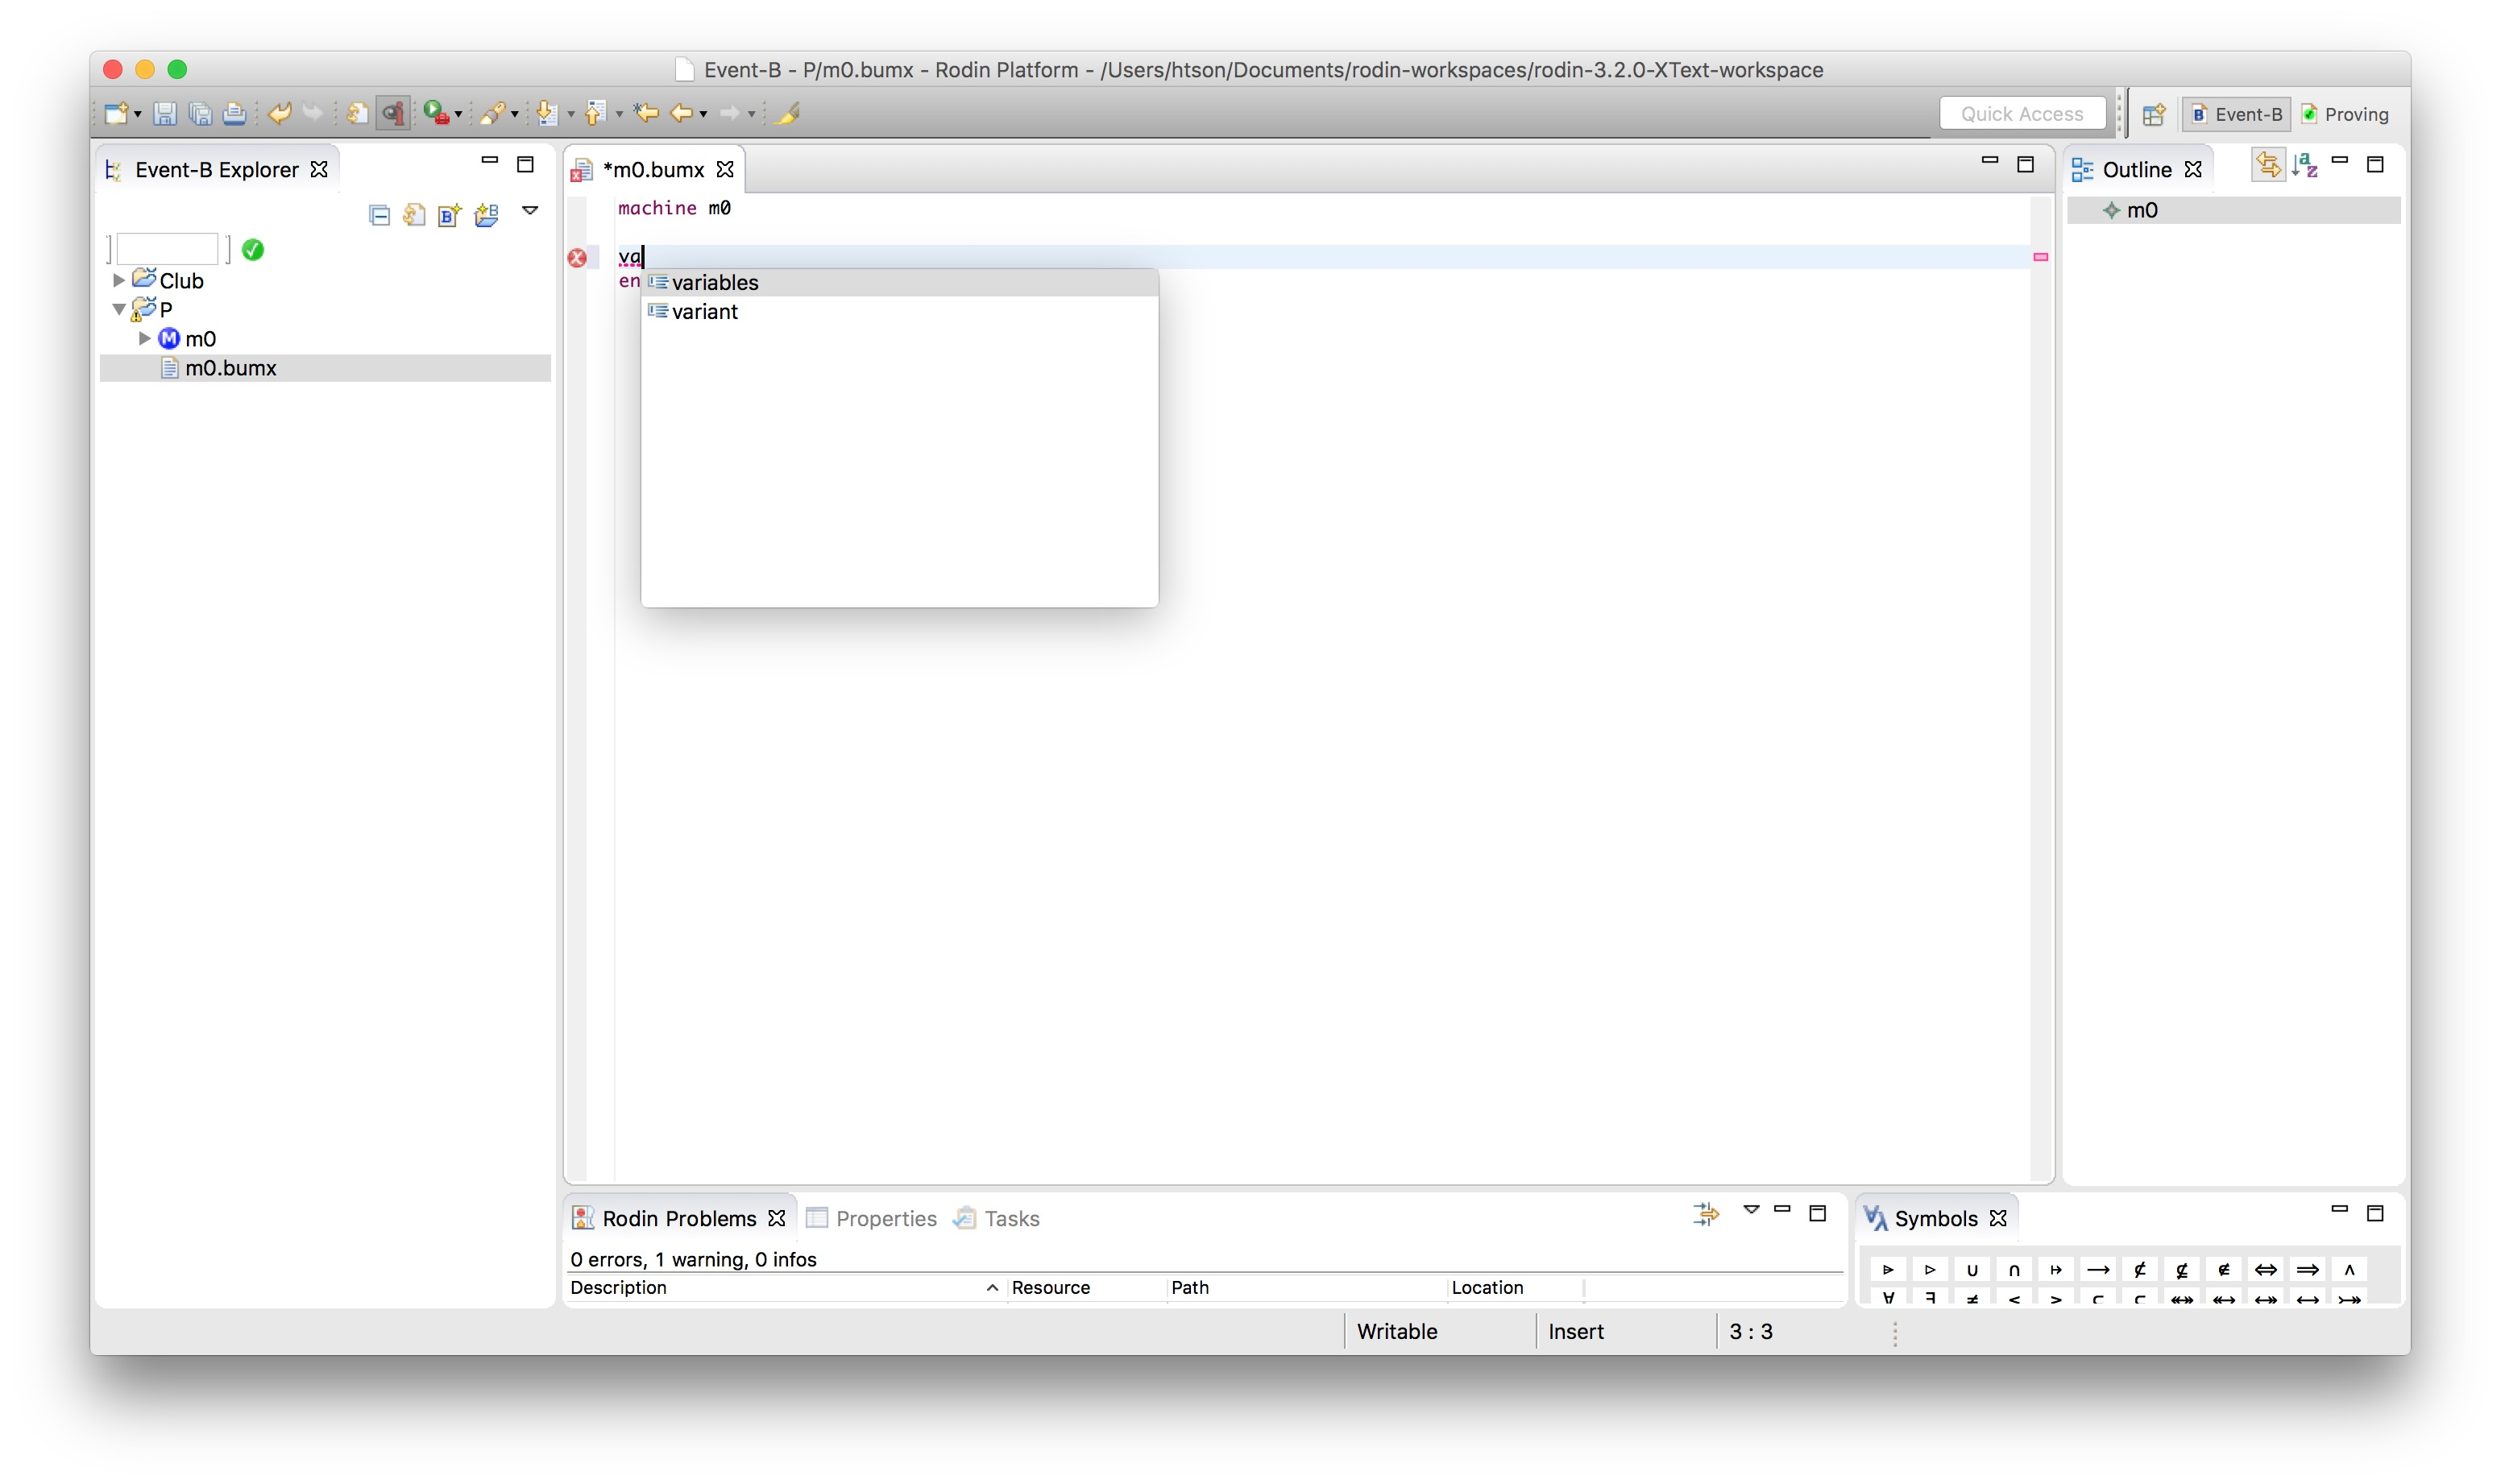
\includegraphics[width=512]{figures/KeywordContentAssist}
  \else
  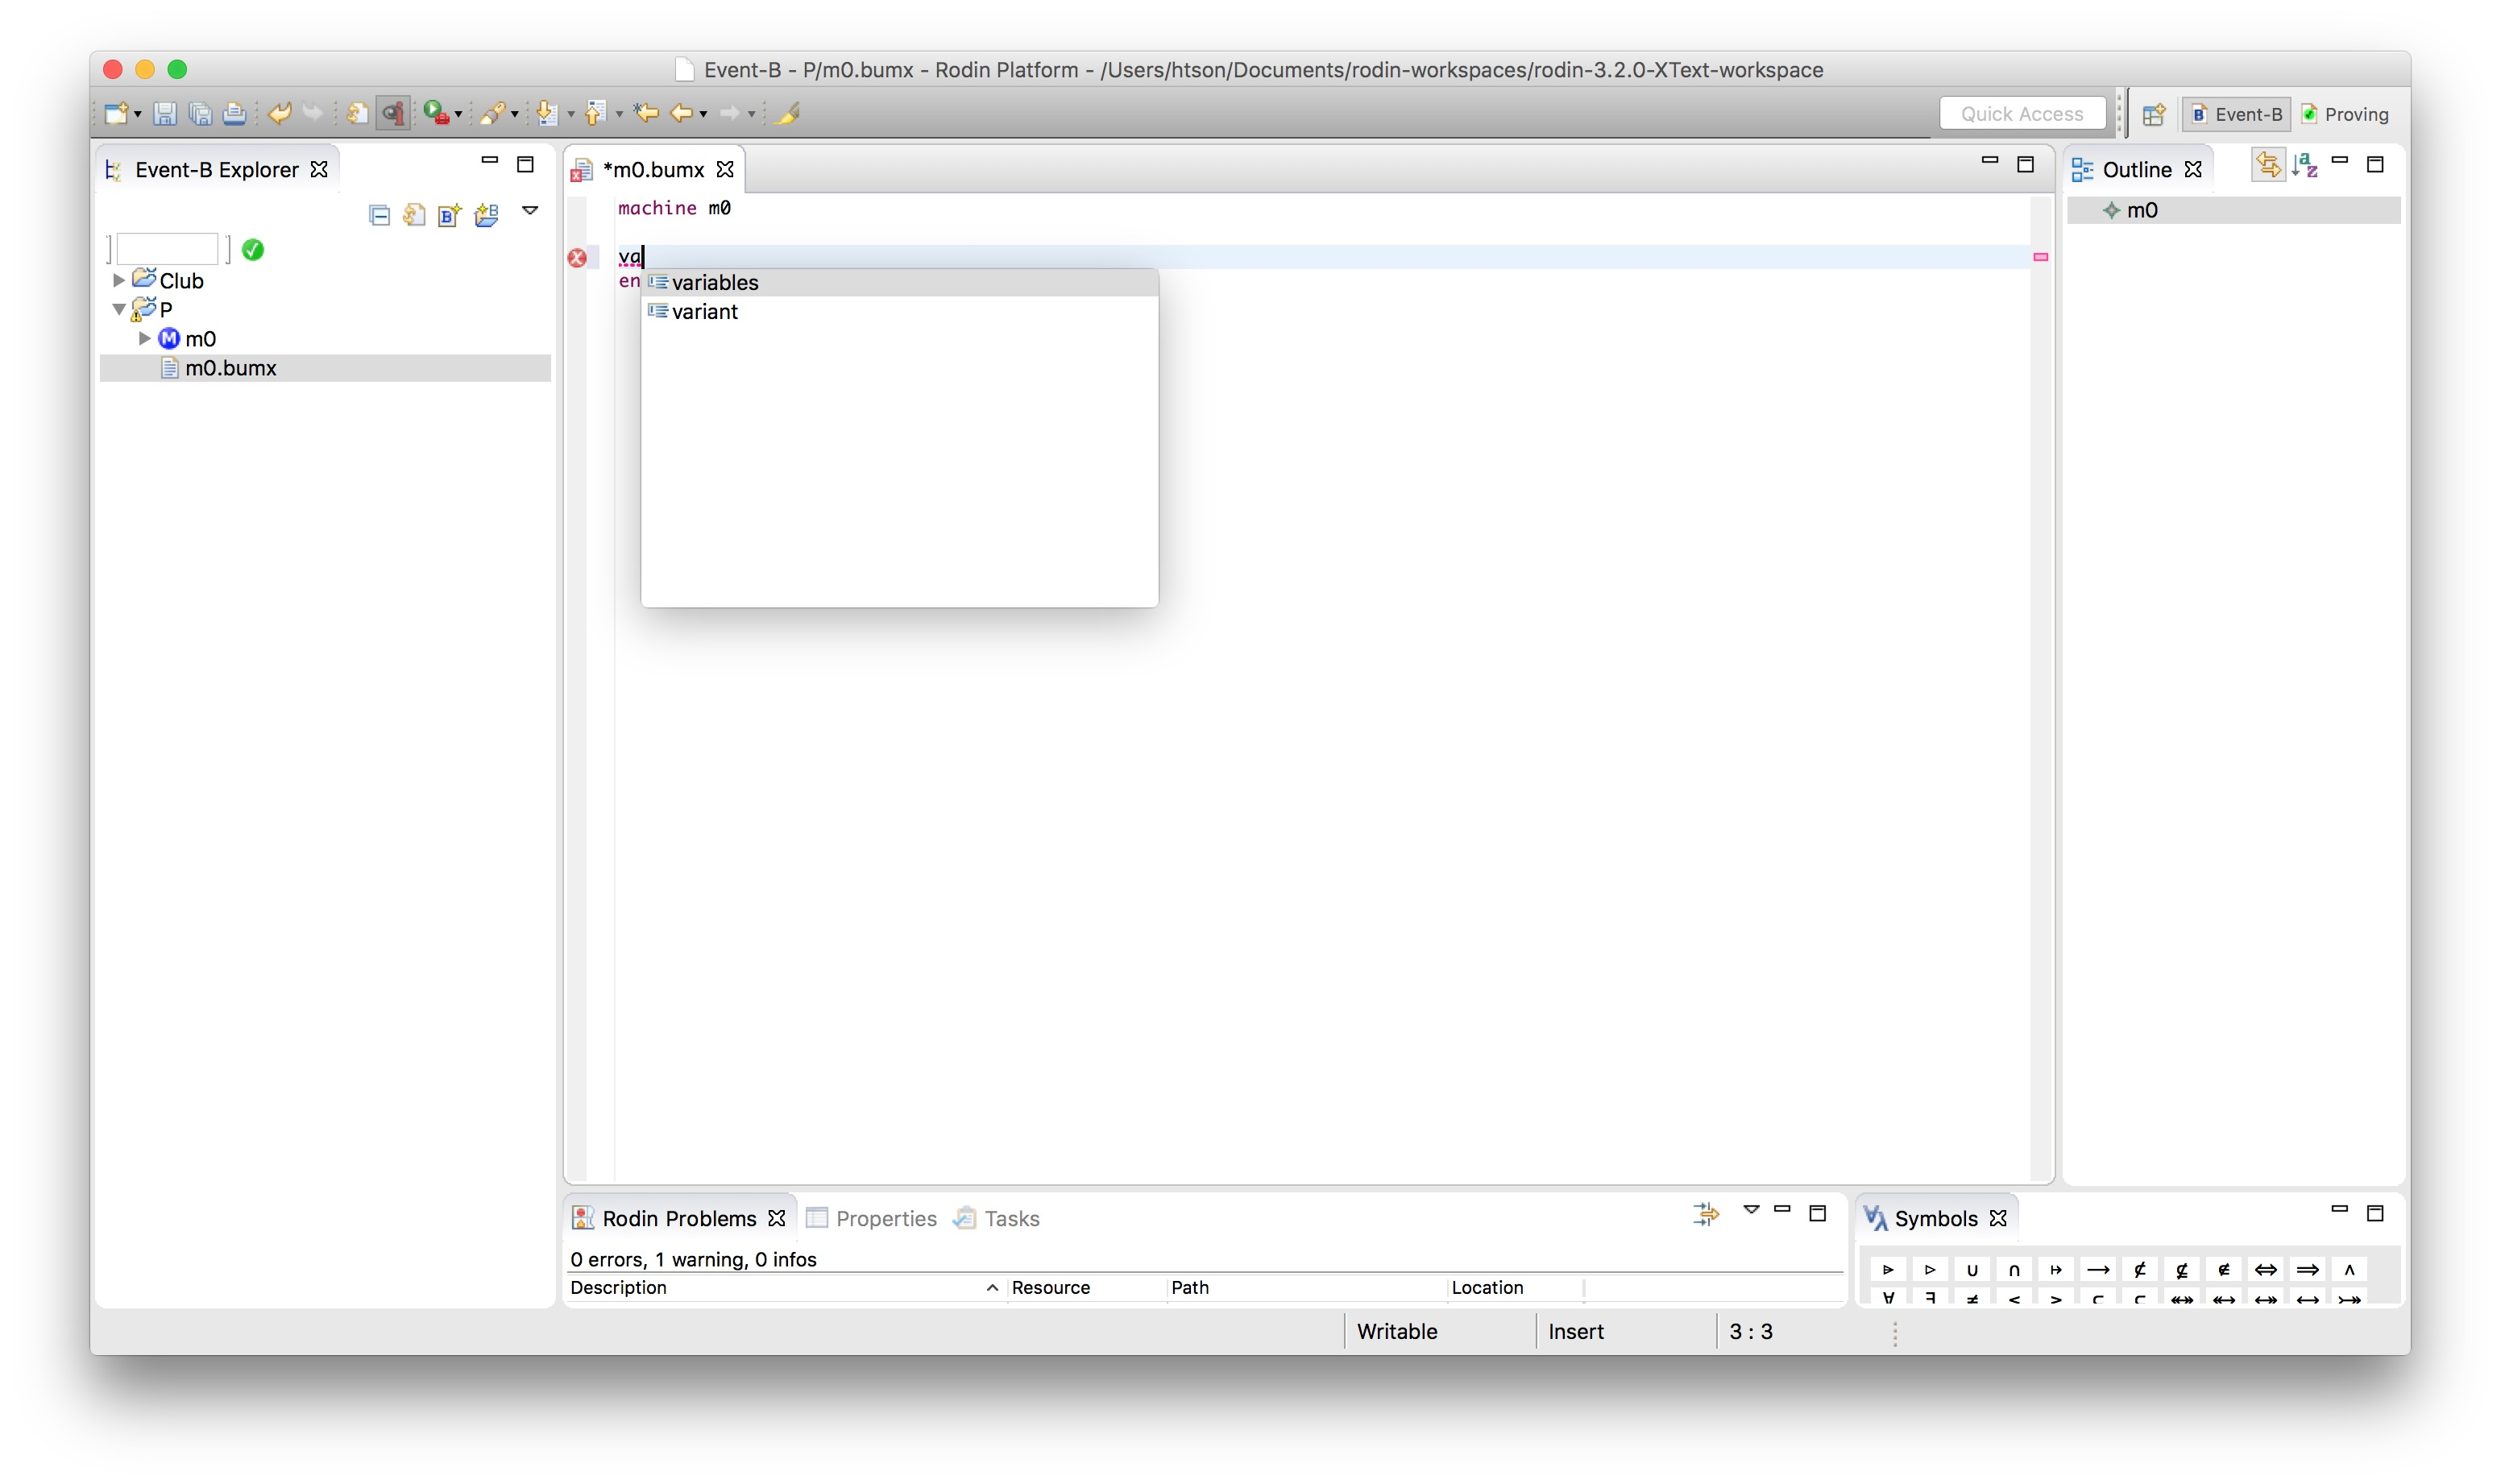
\includegraphics[width=0.9\textwidth]{figures/KeywordContentAssist}
  \fi
  \caption{Keyword Content Assist}
  \label{fig:KeywordContentAssist}
\end{figure}
For Event-B mathematical symbols, the key combination is defined by the Rodin Keyboard plug-in.


%%% Local Variables:
%%% mode: latex
%%% TeX-master: "user_manual"
%%% End:


\section{Tasks}
\label{sec:tasks}

\subsection{Creating XEvent-B Files}
\label{sec:creating-xevent-b}

New XEvent-B files can be create via the \emph{New File wizard} with appropriate file extensions. The file extension for XContext is \texttt{bucx} and for XMachine is \texttt{bumx}.  The syntax of XContext and XMachine can be seen in Section~\ref{sec:xcontext-syntax} and Section~\ref{sec:xmachine-syntax}, respectively.

\subsection{Typesetting Event-B Mathematical Symbols}
\label{sec:typesetting-event-b}
Event-B mathematical symbols in predicates, expressions, and assignments are typeset using Content Assist.  The definition of the character combinations is defined in the Rodin Keyboard plug-in.


%%% Local Variables:
%%% mode: latex
%%% TeX-master: "user_manual"
%%% End:


\section{Reference}
\label{sec:reference}

\subsection{Common Syntax}
\label{sec:common-syntax}
\begin{center}
  \begin{Bcode}
ML_COMMENT ::= /* STRING */\\
SL_COMMENT ::= // SL_STRING \\
ID ::= [^] (LETTER | \_) \{LETTER | DIGIT | \_ \}\\
XLABEL ::= @STRING:\\
  \end{Bcode}
\end{center}


\subsection{XContext Syntax}
\label{sec:xcontext-syntax}

\begin{center}
  \begin{Bcode}
    XCONTEXT ::= \\
    \Btab \Btab [ ML_COMMENT | SL_COMMENT ]\\
    \Btab \Btab \Bcontext{} ID \\
    \Btab \Btab [\Bextends{} ID \{ ID \}]\\
    \Btab \Btab [\Bsets{} XSET \{XSET\}]\\
    \Btab \Btab [\Bconstants{} XCONSTANT \{ XCONSTANT \}]\\
    \Btab \Btab [\Baxioms{} XAXIOM \{XAXIOM\}]\\[2ex]
    \Btab \Btab \Bend\\
    XSET ::= \\
    \Btab \Btab XSET\_NO\_COMMENT | \\
    \Btab \Btab XSET\_ML\_COMMENT | \\
    \Btab \Btab XSET\_SL\_COMMENT \\
    XSET\_NO\_COMMENT ::= ID \\
    XSET\_ML\_COMMENT ::= ML\_COMMENT ID\\
    XSET\_SL\_COMMENT ::= ID ML\_COMMENT\\
    XCONSTANT ::= \\
    \Btab \Btab XCONSTANT\_NO\_COMMENT | \\
    \Btab \Btab XCONSANT\_ML\_COMMENT | \\
    \Btab \Btab XCONSTANT\_SL\_COMMENT \\
    XCONSTANT\_NO\_COMMENT ::= ID \\
    XCONSTANT\_ML\_COMMENT ::= ML\_COMMENT ID\\
    XCONSTANT\_SL\_COMMENT ::= ID ML\_COMMENT\\
    XAXIOM ::= \\
    \Btab \Btab XAXIOM\_NO\_COMMENT | \\
    \Btab \Btab XAXIOM\_ML\_COMMENT | \\
    \Btab \Btab XAXIOM\_SL\_COMMENT \\
    XAXIOM\_NO\_COMMENT ::= XLABEL "XPREDICATE" [\Btheorem]\\
    XAXIOM\_ML\_COMMENT ::= ML\_COMMENT XLABEL "XPREDICATE" [\Btheorem]\\
    XAXIOM\_SL\_COMMENT ::= XLABEL "XPREDICATE" [\Btheorem] SL\_COMMENT\\
  \end{Bcode}
\end{center}

\subsection{XMachine syntax}
\label{sec:xmachine-syntax}
\begin{center}
  \begin{Bcode}
    XMACHINE ::= [ ML_COMMENT | SL_COMMENT ]\\
    \Btab \Btab \Bmachine{} ID \\
    \Btab \Btab [\Brefines{} ID\\
    \Btab \Btab [\Bsees{} ID \{ ID \}\\
    \Btab \Btab [\Bvariables{} XVARIABLE \{XVARIABLE\}]\\
    \Btab \Btab [\Binvariants{} XINVARIANT \{ XINVARIANT \}]\\
    \Btab \Btab [\Bvariant{} XVARIANT]\\
    \Btab \Btab [\Bevents{} XEVENT \{ XEVENT \}] \\
    \Btab \Btab \Bend \\
    XVARIABLE ::= \\
    \Btab \Btab XVARIABLE\_NO\_COMMENT | \\
    \Btab \Btab XVARIABLE\_ML\_COMMENT | \\
    \Btab \Btab XVARIABLE\_SL\_COMMENT \\
    XVARIABLE\_NO\_COMMENT ::= ID \\
    XVARIABLE\_ML\_COMMENT ::= ML\_COMMENT ID \\
    XVARIABLE\_SL\_COMMENT ::= ID SL\_COMMENT \\
    XINVARIANT ::=\\
    \Btab \Btab XINVARIANT\_NO\_COMMENT\\
    \Btab \Btab XINVARIANT\_ML\_COMMENT\\
    \Btab \Btab XINVARIANT\_SL\_COMMENT\\
    XINVARIANT\_NO\_COMMENT ::= \\
    \Btab \Btab XLABEL "XPREDICATE" [\Btheorem] \\
    XINVARIANT\_ML\_COMMENT ::= \\
    \Btab \Btab ML\_COMMENT XLABEL "XPREDICATE" [\Btheorem]\\
    XINVARIANT\_SL\_COMMENT ::= \\
    \Btab \Btab XLABEL "XPREDICATE" [\Btheorem] SL\_COMMENT\\
    XEVENT ::= \\
    \Btab \Btab XEVENT\_NO\_COMMENT\\
    \Btab \Btab XEVENT\_ML\_COMMENT\\
    \Btab \Btab XEVENT\_SL\_COMMENT\\
    XEVENT\_NO\_COMMENT ::=\\
    \Btab \Btab ID \\
    \Btab \Btab ([\Bextended] \& [\Bordinary | \Bconvergent | \Banticipated])\\
    \Btab \Btab [\Brefines{} ID \{ ID \}]\\
    \Btab \Btab [\\
    \Btab \Btab \Btab [\Bwith{} XWITNESS \{ XWITNESS \}] \\
    \Btab \Btab \Btab \Bbegin{} XACTION \{ XACTION \} \\
    \Btab \Btab \Btab | \\
    \Btab \Btab \Btab \Bwhen{} XGUARD \{ XGUARD \}\\
    \Btab \Btab \Btab [\Bwith{} XWITNESS \{ XWITNESS \}] \\
    \Btab \Btab \Btab [\Bthen{} XACTION \{ XACTION \}] \\
    \Btab \Btab \Btab | \\
    \Btab \Btab \Btab \Bany{} XPARAMETER \{ XPARAMETER \}\\
    \Btab \Btab \Btab \Bwhere{} XGUARD \{ XGUARD \}\\
    \Btab \Btab \Btab [\Bwith{} XWITNESS \{ XWITNESS \}] \\
    \Btab \Btab \Btab [\Bthen{} XACTION \{ XACTION \}] \\
    \Btab \Btab ]\\
    \Btab \Btab \Bend\\
    XEVENT\_ML\_COMMENT ::=\\
    \Btab \Btab ML\_COMMENT\\
    \Btab \Btab ID \\
    \Btab \Btab ([\Bextended] \& [\Bordinary | \Bconvergent | \Banticipated])\\
    \Btab \Btab [\Brefines{} ID \{ ID \}]\\
    \Btab \Btab [\\
    \Btab \Btab \Btab [\Bwith{} XWITNESS \{ XWITNESS \}] \\
    \Btab \Btab \Btab \Bbegin{} XACTION \{ XACTION \} \\
    \Btab \Btab \Btab | \\
    \Btab \Btab \Btab \Bwhen{} XGUARD \{ XGUARD \}\\
    \Btab \Btab \Btab [\Bwith{} XWITNESS \{ XWITNESS \}] \\
    \Btab \Btab \Btab [\Bthen{} XACTION \{ XACTION \}] \\
    \Btab \Btab \Btab | \\
    \Btab \Btab \Btab \Bany{} XPARAMETER \{ XPARAMETER \}\\
    \Btab \Btab \Btab \Bwhere{} XGUARD \{ XGUARD \}\\
    \Btab \Btab \Btab [\Bwith{} XWITNESS \{ XWITNESS \}] \\
    \Btab \Btab \Btab [\Bthen{} XACTION \{ XACTION \}] \\
    \Btab \Btab ]\\
    \Btab \Btab \Bend\\
    XEVENT\_SL\_COMMENT ::=\\
    \Btab \Btab ID \\
    \Btab \Btab ([\Bextended] \& [\Bordinary | \Bconvergent | \Banticipated])\\
    \Btab \Btab [\Brefines{} ID \{ ID \}]\\
    \Btab \Btab SL\_COMMENT\\
    \Btab \Btab [\\
    \Btab \Btab \Btab [\Bwith{} XWITNESS \{ XWITNESS \}] \\
    \Btab \Btab \Btab \Bbegin{} XACTION \{ XACTION \} \\
    \Btab \Btab \Btab | \\
    \Btab \Btab \Btab \Bwhen{} XGUARD \{ XGUARD \}\\
    \Btab \Btab \Btab [\Bwith{} XWITNESS \{ XWITNESS \}] \\
    \Btab \Btab \Btab [\Bthen{} XACTION \{ XACTION \}] \\
    \Btab \Btab \Btab | \\
    \Btab \Btab \Btab \Bany{} XPARAMETER \{ XPARAMETER \}\\
    \Btab \Btab \Btab \Bwhere{} XGUARD \{ XGUARD \}\\
    \Btab \Btab \Btab [\Bwith{} XWITNESS \{ XWITNESS \}] \\
    \Btab \Btab \Btab [\Bthen{} XACTION \{ XACTION \}] \\
    \Btab \Btab ]\\
    \Btab \Btab \Bend\\
    XWITNESS ::= \\
    \Btab \Btab XWITNESS\_NO\_COMMENT | \\
    \Btab \Btab XWITNESS\_ML\_COMMENT | \\
    \Btab \Btab XWITNESS\_SL\_COMMENT | \\
    XWITNESS\_NO\_COMMENT ::= XLABEL "XPREDICATE" \\
    XWITNESS\_ML\_COMMENT ::= ML\_COMMENT XLABEL "XPREDICATE" \\
    XWITNESS\_SL\_COMMENT ::= XLABEL "XPREDICATE" SL\_COMMENT \\
    XPARAMETER ::= \\
    \Btab \Btab XPARAMETER\_NO\_COMMENT | \\
    \Btab \Btab XPARAMETER\_ML\_COMMENT | \\
    \Btab \Btab XPARAMETER\_SL\_COMMENT \\
    XPARAMETER\_NO\_COMMENT ::= ID \\
    XPARAMETER\_ML\_COMMENT ::= ML\_COMMENT ID \\
    XPARAMETER\_SL\_COMMENT ::= ID SL\_COMMENT \\
    XGUARD ::=\\
    \Btab \Btab XGUARD\_NO\_COMMENT |\\
    \Btab \Btab XGUARD\_ML\_COMMENT |\\
    \Btab \Btab XGUARD\_SL\_COMMENT\\
    XGUARD\_NO\_COMMENT ::= \\
    \Btab \Btab XLABEL "XPREDICATE" [\Btheorem]\\
    XGUARD\_ML\_COMMENT ::= \\
    \Btab \Btab ML\_COMMENT XLABEL "XPREDICATE" [\Btheorem]\\
    XGUARD\_SL\_COMMENT ::= \\
    \Btab \Btab XLABEL "XPREDICATE" [\Btheorem] SL\_COMMENT\\
    XACTION ::=\\
    \Btab \Btab XACTION\_NO\_COMMENT |\\
    \Btab \Btab XACTION\_ML\_COMMENT |\\
    \Btab \Btab XACTION\_SL\_COMMENT\\
    XACTION\_NO\_COMMENT ::= XLABEL "XASSIGNMENT" [\Btheorem]\\
    XACTION\_ML\_COMMENT ::= ML\_COMMENT XLABEL "XASSIGNMENT"\\
    XACTION\_SL\_COMMENT ::= XLABEL "XASSIGNMENT" SL\_COMMENT
  \end{Bcode}
\end{center}

\subsection{Preferences}
\label{sec:preferences}

\subsubsection{XContext Preferences}
\label{sec:xcontext-preferences}
The following XContext preferences can be set on the  the XContext preference page and its sub-pages.

\paragraph{Compiler}
\begin{table}[!htbp]
  \centering
  \begin{tabular}{|p{0.2\textwidth}|p{0.5\textwidth}|p{0.3\textwidth}|}
    \hline
    \multicolumn{1}{|c}{\textbf{Option}} & \multicolumn{1}{|c}{\textbf{Description}} &%
                                                                                       \multicolumn{1}{|c|}{\textbf{Default}} \\
    \hline
    Compiler is activated & \textbf{Compiler is activated} or \textbf{deactivated} & Activated \\
    \hline
  \end{tabular}
  \caption{XContext Compiler Preferences}
  \label{tab:xcontext-compiler-preference}
\end{table}

\paragraph{Syntax Coloring}
\begin{table}[!htbp]
  \centering
  \begin{tabular}{|p{0.2\textwidth}|p{0.5\textwidth}|p{0.3\textwidth}|}
    \hline
    \multicolumn{1}{|c}{\textbf{Option}} & \multicolumn{1}{|c}{\textbf{Description}} &%
                                                                                       \multicolumn{1}{|c|}{\textbf{Default}} \\
    \hline
    Comment & \textbf{Color} & Dark Green \\
                                         & \textbf{Background} & White \\
                                         & \textbf{Style} (Italic, Bold, Underline, Strike through) & None \\
                                         & \textbf{Font} & Platform dependent \\
    \hline
    Default & \textbf{Color} & Black \\
                                         & \textbf{Background} & White \\
                                         & \textbf{Style} (Italic, Bold, Underline, Strike through) & None \\
                                         & \textbf{Font} & Platform dependent \\
    \hline
    Invalid Symbol & \textbf{Color} & Black \\
                                         & \textbf{Background} & White \\
                                         & \textbf{Style} (Italic, Bold, Underline, Strike through) & None \\
                                         & \textbf{Font} & Platform dependent \\
    \hline
    Keyword & \textbf{Color} & Dark Purple \\
                                         & \textbf{Background} & White \\
                                         & \textbf{Style} (Italic, Bold, Underline, Strike through) & Bold \\
                                         & \textbf{Font} & Platform dependent \\
    \hline
    Number & \textbf{Color} & Dark Gray \\
                                         & \textbf{Background} & White \\
                                         & \textbf{Style} (Italic, Bold, Underline, Strike through) & None \\
                                         & \textbf{Font} & Platform dependent \\
    \hline
    Punctuation character & \textbf{Color} & Black \\
                                         & \textbf{Background} & White \\
                                         & \textbf{Style} (Italic, Bold, Underline, Strike through) & None \\
                                         & \textbf{Font} & Platform dependent \\
    \hline
    String & \textbf{Color} & Blue \\
                                         & \textbf{Background} & White \\
                                         & \textbf{Style} (Italic, Bold, Underline, Strike through) & None \\
                                         & \textbf{Font} & Platform dependent \\
    \hline
    Task Tag & \textbf{Color} & Light Blue \\
                                         & \textbf{Background} & White \\
                                         & \textbf{Style} (Italic, Bold, Underline, Strike through) & Bold \\
                                         & \textbf{Font} & Platform dependent \\
    \hline
  \end{tabular}
  \caption{XContext Syntax Coloring Preferences}
  \label{tab:xcontext-syntax-coloring-preference}
\end{table}


\subsubsection{XMachine Preferences}
\label{sec:xmachine-preferences}
The following XMachine preferences can be set on the  XMachine preference page and its sub-pages.

\paragraph{Compiler}
\begin{table}[!htbp]
  \centering
  \begin{tabular}{|p{0.2\textwidth}|p{0.5\textwidth}|p{0.3\textwidth}|}
    \hline
    \multicolumn{1}{|c}{\textbf{Option}} & \multicolumn{1}{|c}{\textbf{Description}} &%
                                                                                       \multicolumn{1}{|c|}{\textbf{Default}} \\
    \hline
    Compiler is activated & \textbf{Compiler is activated} or \textbf{deactivated} & Activated \\
    \hline
  \end{tabular}
  \caption{XMachine Compiler Preferences}
  \label{tab:xmachine-compiler-preference}
\end{table}

\paragraph{Syntax Coloring}
\begin{table}[!htbp]
  \centering
  \begin{tabular}{|p{0.2\textwidth}|p{0.5\textwidth}|p{0.3\textwidth}|}
    \hline
    \multicolumn{1}{|c}{\textbf{Option}} & \multicolumn{1}{|c}{\textbf{Description}} &%
                                                                                       \multicolumn{1}{|c|}{\textbf{Default}} \\
    \hline
    Comment & \textbf{Color} & Dark Green \\
                                         & \textbf{Background} & White \\
                                         & \textbf{Style} (Italic, Bold, Underline, Strike through) & None \\
                                         & \textbf{Font} & Platform dependent \\
    \hline
    Default & \textbf{Color} & Black \\
                                         & \textbf{Background} & White \\
                                         & \textbf{Style} (Italic, Bold, Underline, Strike through) & None \\
                                         & \textbf{Font} & Platform dependent \\
    \hline
    Invalid Symbol & \textbf{Color} & Black \\
                                         & \textbf{Background} & White \\
                                         & \textbf{Style} (Italic, Bold, Underline, Strike through) & None \\
                                         & \textbf{Font} & Platform dependent \\
    \hline
    Keyword & \textbf{Color} & Dark Purple \\
                                         & \textbf{Background} & White \\
                                         & \textbf{Style} (Italic, Bold, Underline, Strike through) & Bold \\
                                         & \textbf{Font} & Platform dependent \\
    \hline
    Number & \textbf{Color} & Dark Gray \\
                                         & \textbf{Background} & White \\
                                         & \textbf{Style} (Italic, Bold, Underline, Strike through) & None \\
                                         & \textbf{Font} & Platform dependent \\
    \hline
    Punctuation character & \textbf{Color} & Black \\
                                         & \textbf{Background} & White \\
                                         & \textbf{Style} (Italic, Bold, Underline, Strike through) & None \\
                                         & \textbf{Font} & Platform dependent \\
    \hline
    String & \textbf{Color} & Blue \\
                                         & \textbf{Background} & White \\
                                         & \textbf{Style} (Italic, Bold, Underline, Strike through) & None \\
                                         & \textbf{Font} & Platform dependent \\
    \hline
    Task Tag & \textbf{Color} & Light Blue \\
                                         & \textbf{Background} & White \\
                                         & \textbf{Style} (Italic, Bold, Underline, Strike through) & Bold \\
                                         & \textbf{Font} & Platform dependent \\
    \hline
  \end{tabular}
  \caption{XMachine Syntax Coloring Preferences}
  \label{tab:xmachine-syntax-coloring-preference}
\end{table}

\subsection{XEvent-B Editors}
\label{sec:xevent-b-editors}


\subsubsection{XEvent-B Content Assist}
\label{sec:xevent-b-content}
In the XContext and XMachine editors press \texttt{Ctrl+Space} on code to complete. This opens a list of available code completions. Some tips for using code assist are listed in the following paragraph:
\begin{itemize}
\item You can use the mouse or the keyboard (Up Arrow, Down Arrow, Page Up, Page Down, Home, End, Enter) to navigate and select lines in the list.

\item Clicking or pressing Enter on a selected line in the list inserts the selection into the editor.
\end{itemize}
\begin{figure}[!htbp]
  \centering
  \ifplastex
  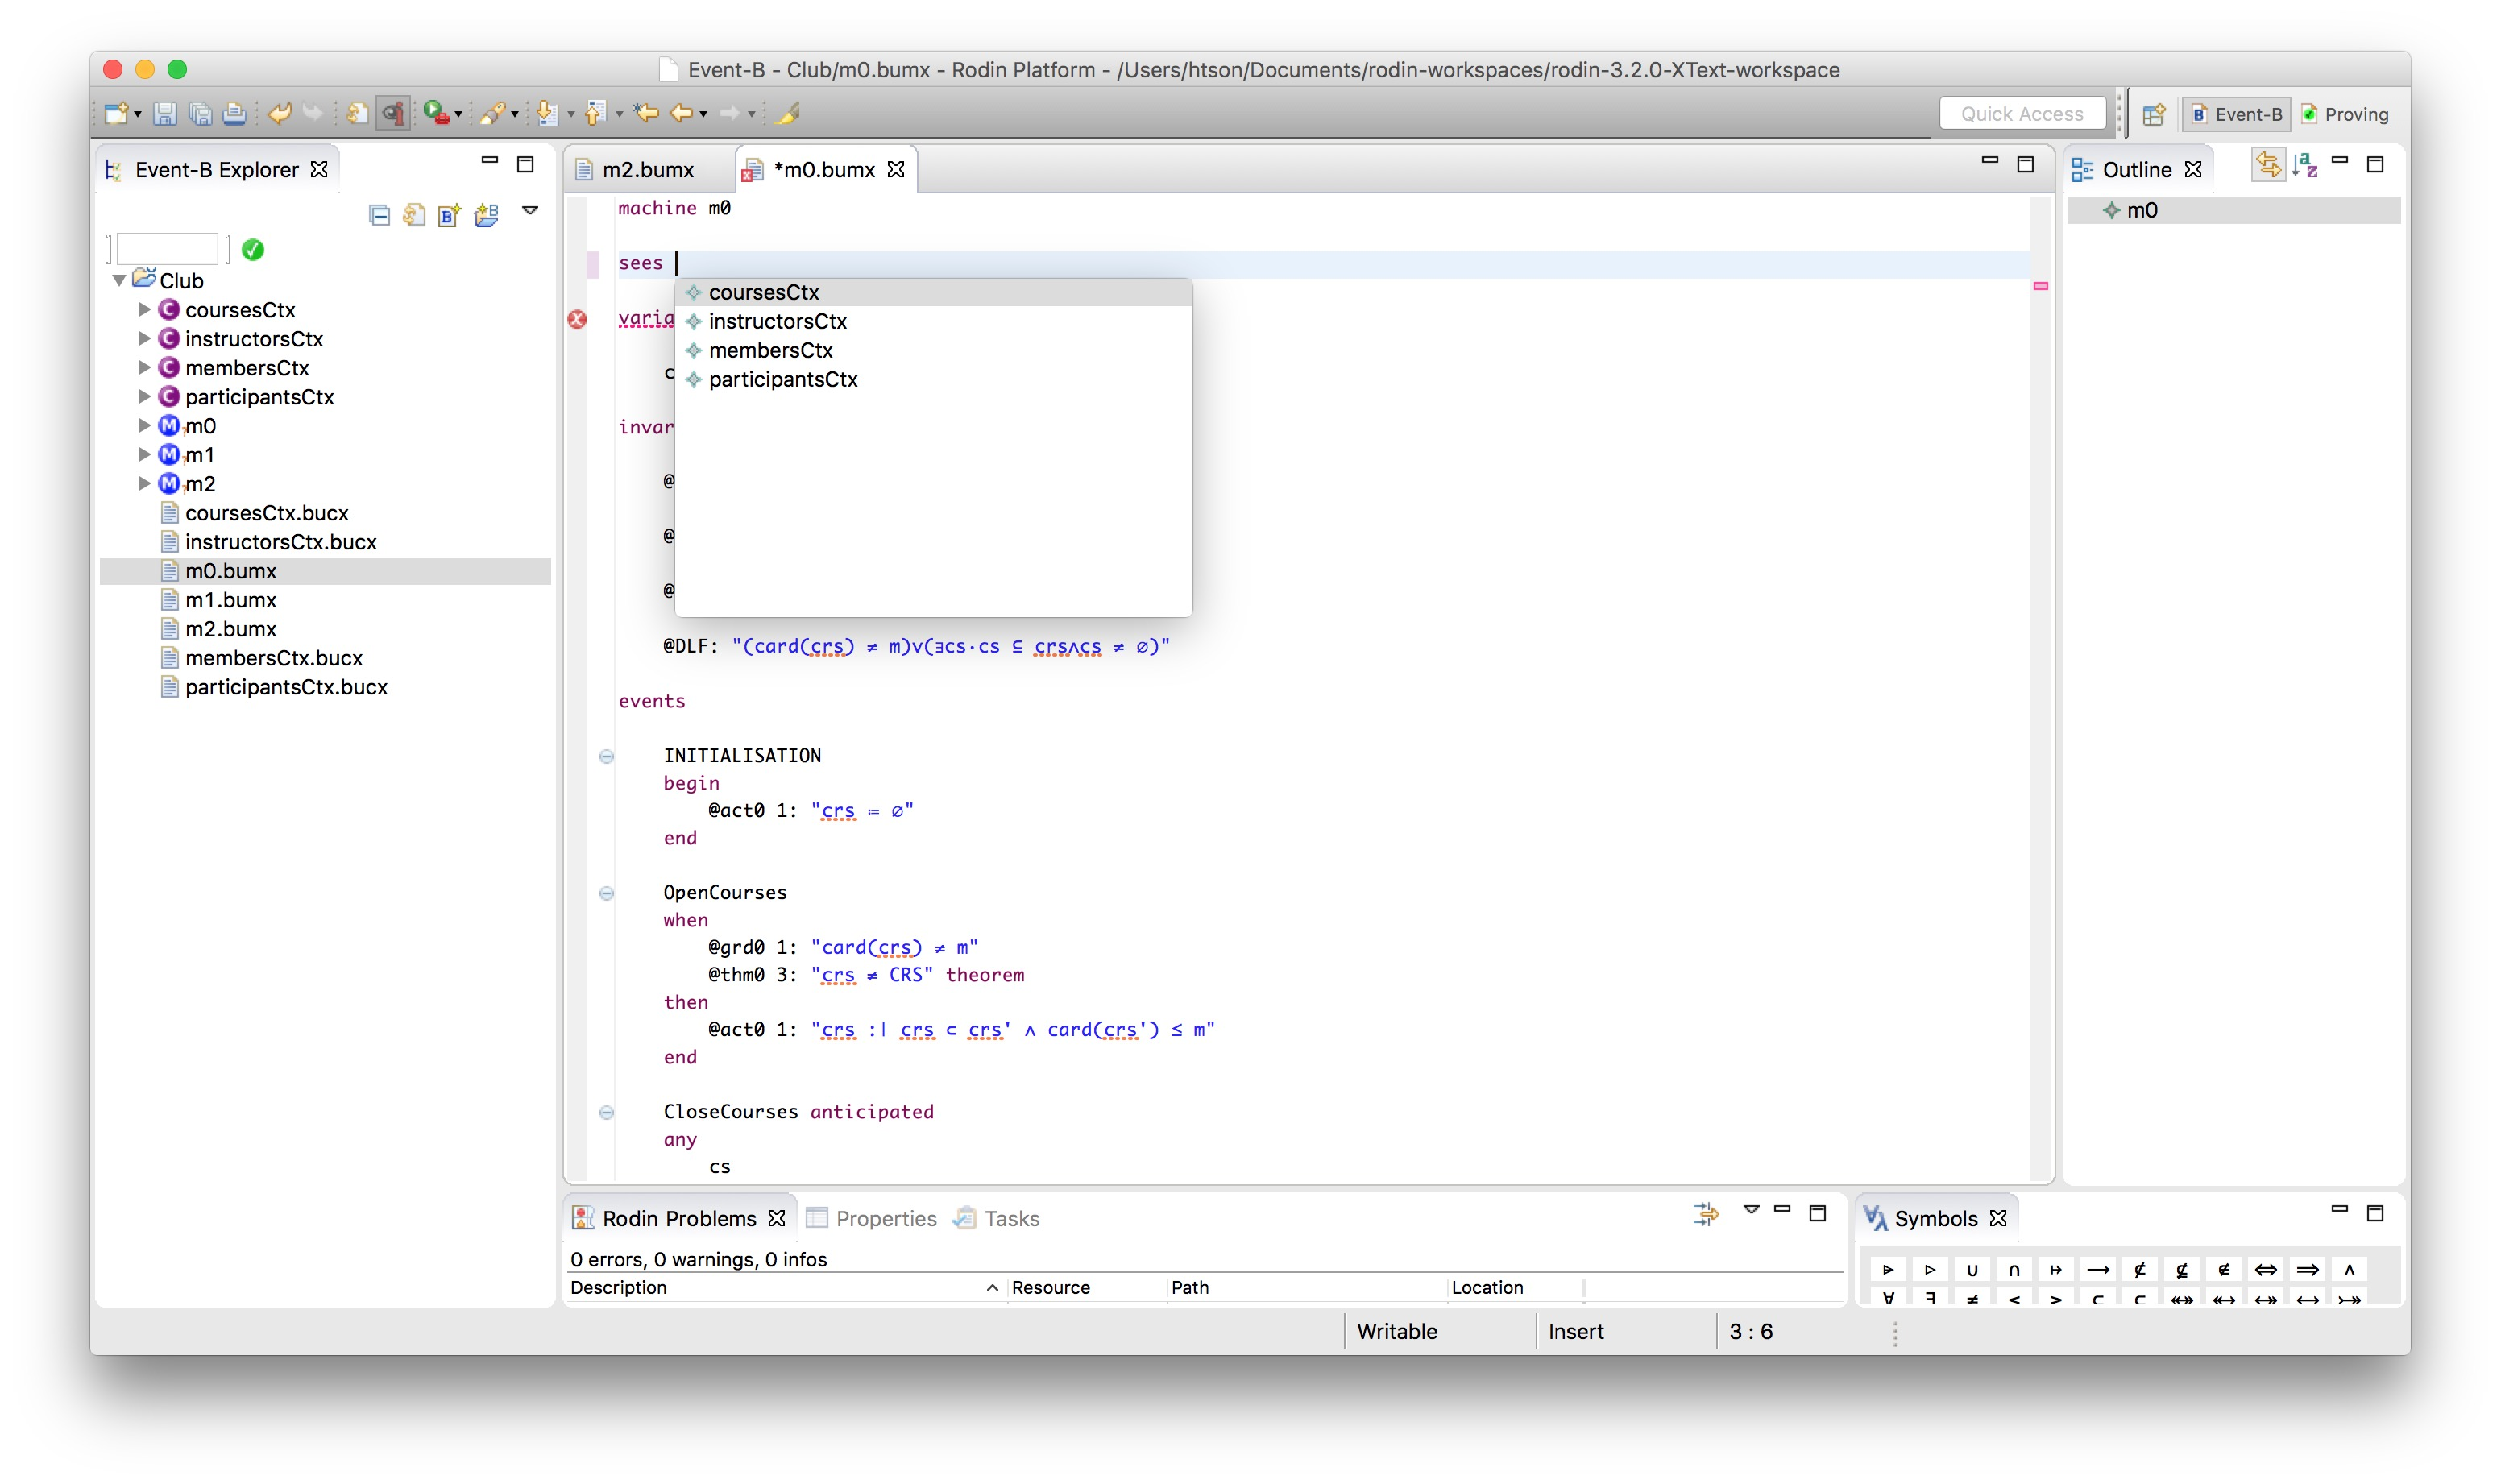
\includegraphics[width=512]{figures/SeesContentAssist}
  \else
  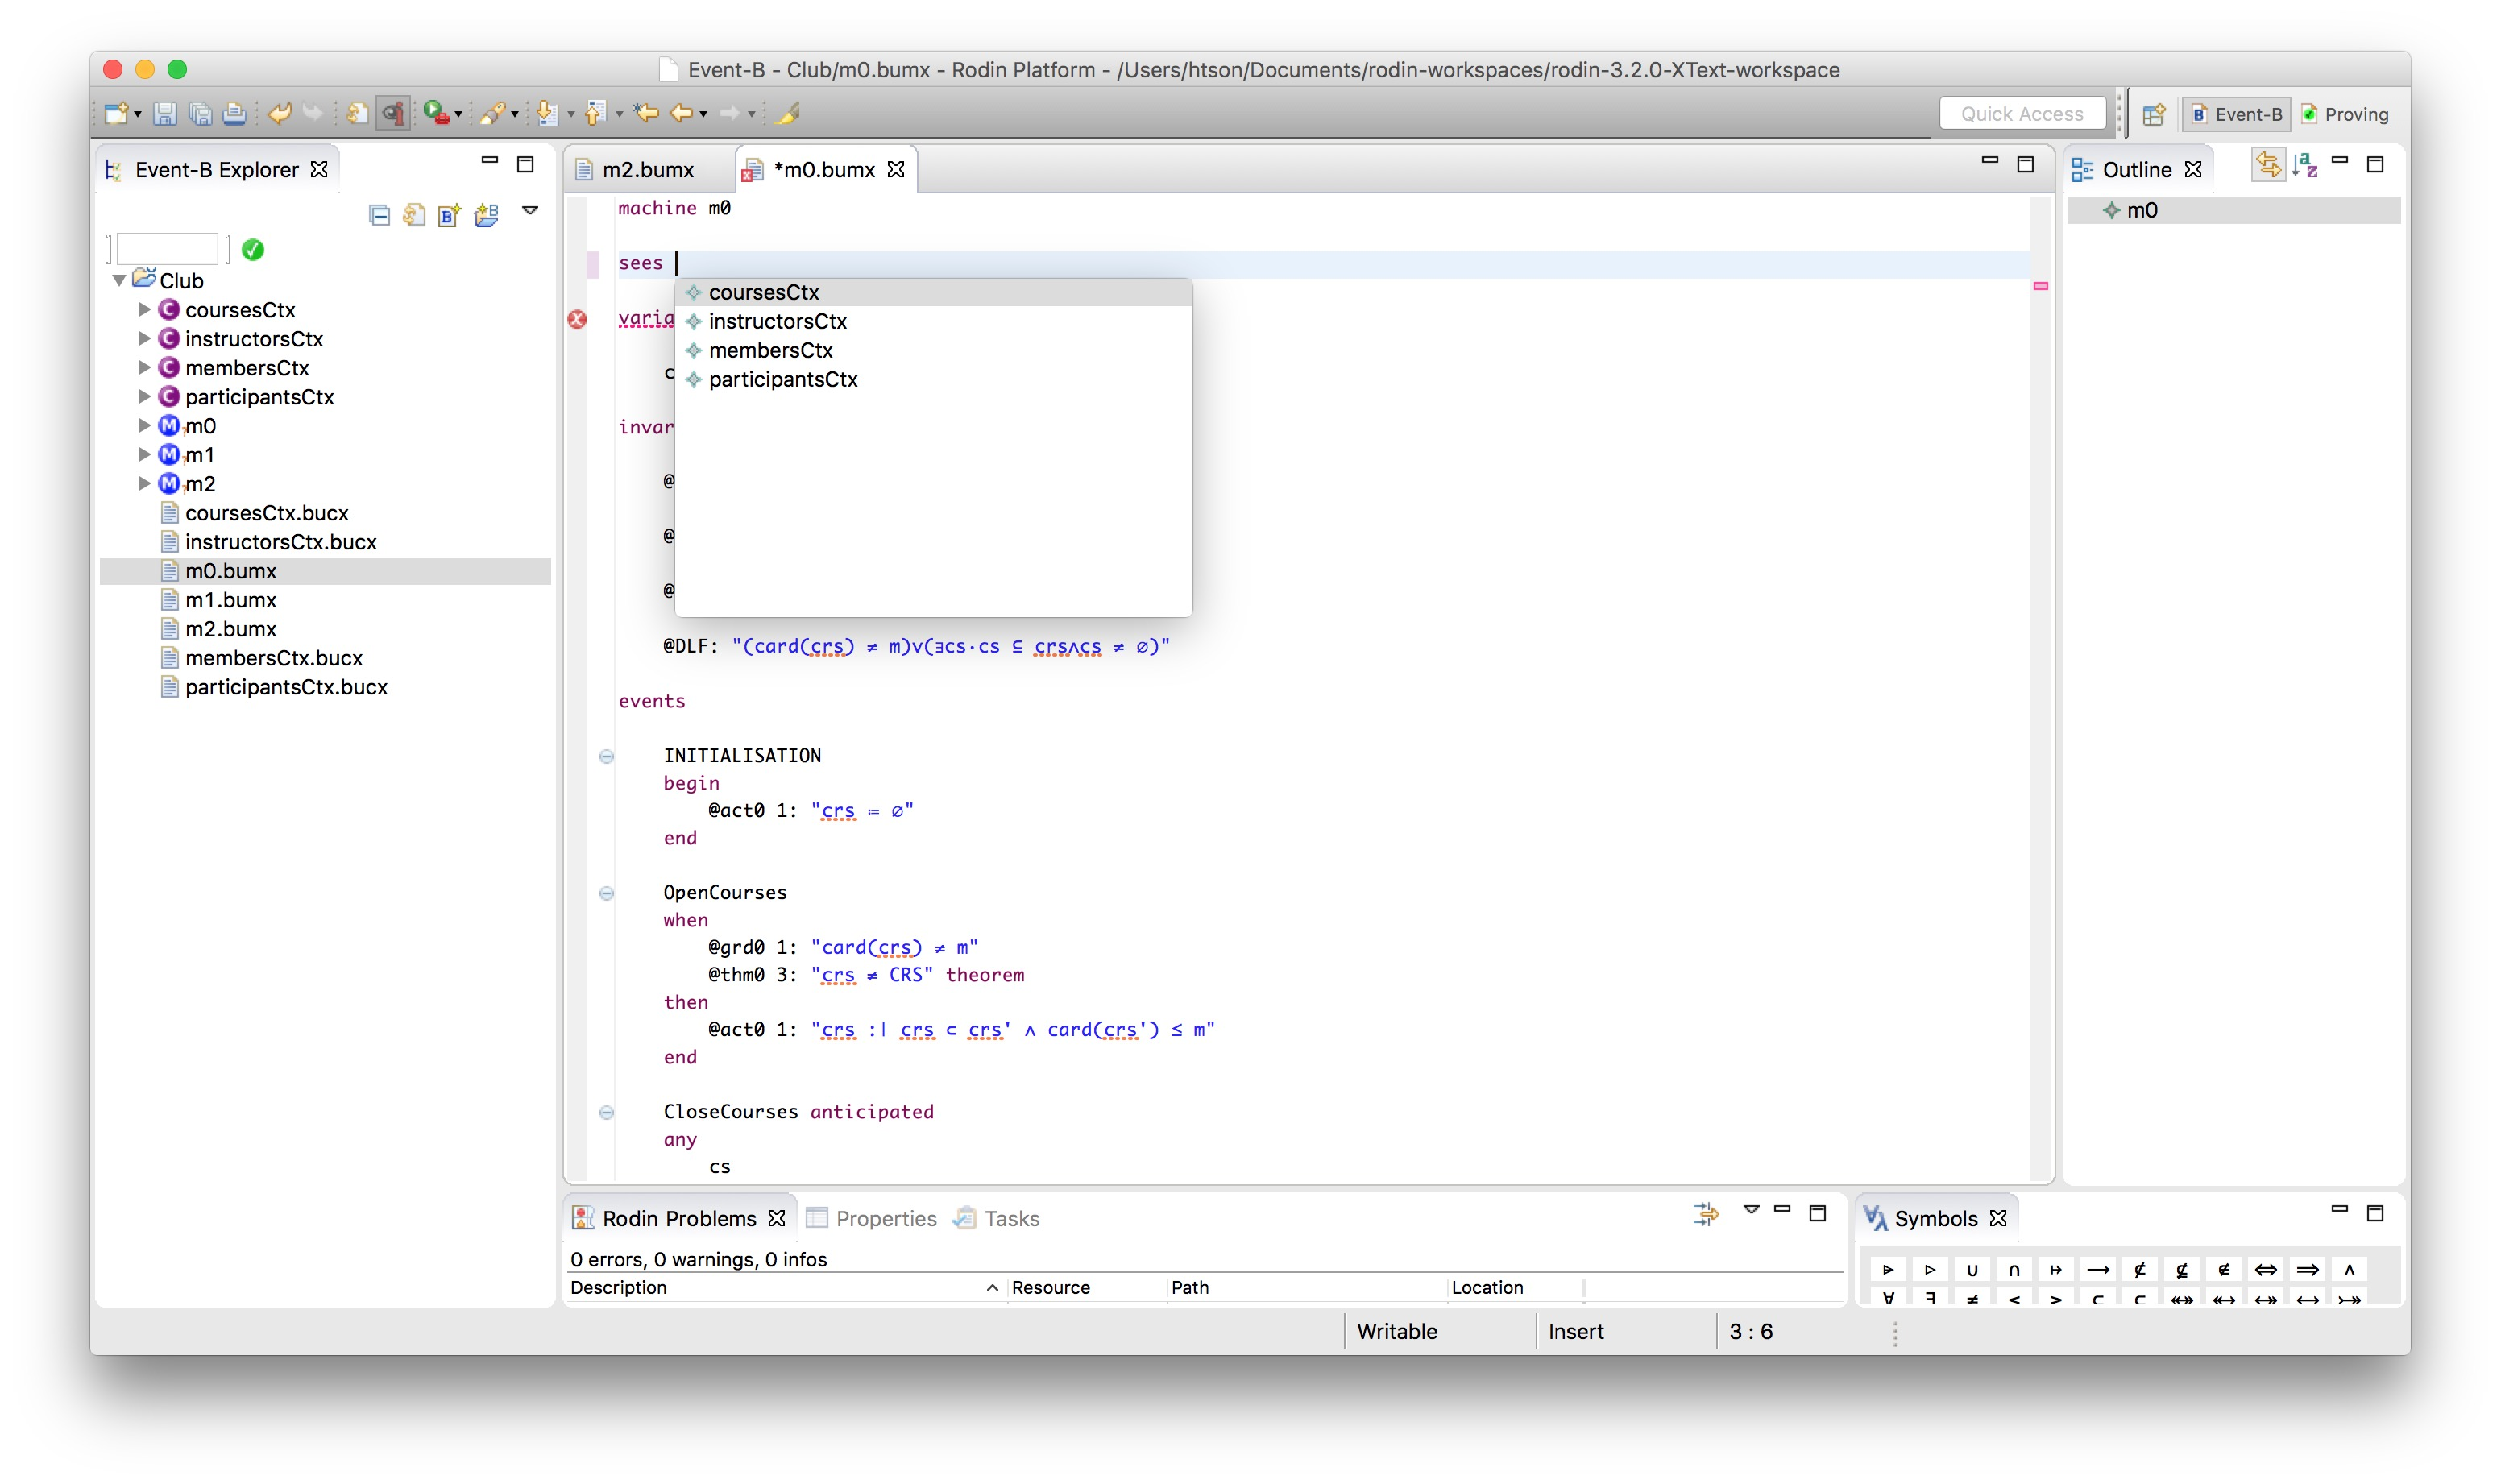
\includegraphics[width=0.9\textwidth]{figures/SeesContentAssist}
  \fi
  \caption{Content Assist for adding Sees clause}
  \label{fig:SeesContentAssist}
\end{figure}

\subsubsection{XEvent-B Formatter}
\label{sec:xevent-b-formatter}
In the XContent and XMachine editors press \texttt{Ctrl+Shift+F} on code to format it. If no selection is set then the entire source is formatted otherwise only the selection will be. 

%%% Local Variables:
%%% mode: latex
%%% TeX-master: "user_manual"
%%% End:


%\section{Samples}
\label{sec:samples}


%%% Local Variables:
%%% mode: latex
%%% TeX-master: "user_manual"
%%% End:


\ifplastex
\section{Legal}
\label{sec:legal}

\subsection{RODIN Software User Agreement}
\label{sec:user-agreement}

February 2nd, 2016

\ifplastex
\subsubsection{Usage Of Content}
\label{sec:usage-content}
\else
  \ifstandalone
  \subsubsection{Usage Of Content}
  \label{sec:usage-content}
  \else
  \section{Usage Of Content}
  \label{sec:usage-content}
  \fi
\fi

All intellectual property rights existing in this information remain
the property of the Secretary of State for Defence of the United
Kingdom of Great Britain and Northern Ireland. The information may not
be used or disclosed otherwise that is provided for by the
above-mentioned licence without the prior written permission of the
Secretary of State, as represented by the Copyright Unit, Defence
Intellectual Property Rights, Poplar 2 \#2214, MOD Abbey Wood South,
Bristol BS34 8JH, UNITED KINGDOM.

CODA is provided on the basis that the US Government will disclose to
the UK Ministry of Defence (via AWE) any information, test results,
modifications or further developments based on or derived from the
disclosed information and will authorise the use of such information
for UK Government purposes on the same terms (i.e. under the terms of
the Creative Commons Attribution-NonCommercial- ShareAlike 4.0
International License (CC BY NC SA 4.0)).

For the avoidance of doubt, the Secretary of State of Defence for the
United Kingdom of Great Britain and Northern Ireland does not provide
any indemnity, and does not warrant the accuracy or completeness of
the information, nor does it warrant the suitability or completeness
of the information for any particular use or application.

Any requests for further use or disclosure of the information should,
in the first instance, be directed to AWE Commercial (via the Formal
Methods team at AWE).

\ifplastex
\subsubsection{Applicable Licences}
\label{sec:vhdl-applicable-licences}
\else
  \ifstandalone
  \subsubsection{Applicable Licences}
  \label{sec:vhdl-applicable-licences}
  \else
  \section{Applicable Licences}
  \label{sec:vhdl-applicable-licences}
  \fi
\fi
 
Unless otherwise indicated, all Content made available by the CODA
project is provided to you under the terms and conditions of one of
the following licences.

\begin{itemize}
\item The \emph{Creative Commons Attribution-NonCommercial-ShareAlike 4.0
    International License} (CC BY NC SA 4.0).  A copy of the \emph{CC BY NC SA
    4.0} is available at \url{https://creativecommons.org/licenses/by-nc-sa/4.0/legalcode}.

\item \emph{Eclipse Public License Version 1.0} (EPL) (available at 
   \url{http://www.eclipse.org/legal/epl-v10.html})
\end{itemize}

Content includes, but is not limited to, source code, object code,
documentation and other files maintained in the CODA repository (``Repository'').

The terms and conditions governing Features and Included Features
should be contained in files named ``licence.html'' (``Feature
Licences'').  Feature Licences may be located in any directory of a
Download or Module including, but not limited to the following
locations:

\begin{itemize}
\item Feature directories

\item Shared-licence feature \texttt{ac.soton.coda.licence}
\end{itemize}

Note: if a Feature made available by the CODA Project is
installed using the Eclipse Update Manager, you must agree to a
licence (``Feature Update Licence'') during the installation process.
If the Feature contains Included Features, the Feature Update
Licence should either provide you with the terms and conditions
governing the Included Features or inform you where you can locate
them.  Feature Update Licences may be found in the ``licence''
property of files named ``feature.properties'' found within a
Feature.  Such Feature Licences, and Feature Update
Licences contain the terms and conditions (or references to such
terms and conditions) that govern your use of the associated
Content in that directory.

THE FEATURE LICENCES, AND FEATURE UPDATE LICENCES MAY REFER
TO THE CC BY NC SA 4.0, EPL OR OTHER LICENCE AGREEMENTS, NOTICES OR TERMS AND
CONDITIONS.

IT IS YOUR OBLIGATION TO READ AND ACCEPT ALL SUCH TERMS AND
CONDITIONS PRIOR TO USE OF THE CONTENT.  If no Feature
Licence, or Feature Update Licence is provided, please contact the
CODA Project to determine what terms and conditions govern
that particular Content.
\begin{quote}
  \footnotesize

  \begin{itemize}
  \item  Java and all Java-based trademarks are trademarks of Sun
    Microsystems, Inc. in the United States, other countries, or
    both.
  \end{itemize}
\end{quote}

%%% Local Variables:
%%% mode: latex
%%% TeX-master: "user_manual"
%%% End:

\else
  \ifstandalone
  \section{Legal}
  \label{sec:legal}

  \subsection{RODIN Software User Agreement}
  \label{sec:user-agreement}

  February 2nd, 2016

\ifplastex
\subsubsection{Usage Of Content}
\label{sec:usage-content}
\else
  \ifstandalone
  \subsubsection{Usage Of Content}
  \label{sec:usage-content}
  \else
  \section{Usage Of Content}
  \label{sec:usage-content}
  \fi
\fi

All intellectual property rights existing in this information remain
the property of the Secretary of State for Defence of the United
Kingdom of Great Britain and Northern Ireland. The information may not
be used or disclosed otherwise that is provided for by the
above-mentioned licence without the prior written permission of the
Secretary of State, as represented by the Copyright Unit, Defence
Intellectual Property Rights, Poplar 2 \#2214, MOD Abbey Wood South,
Bristol BS34 8JH, UNITED KINGDOM.

CODA is provided on the basis that the US Government will disclose to
the UK Ministry of Defence (via AWE) any information, test results,
modifications or further developments based on or derived from the
disclosed information and will authorise the use of such information
for UK Government purposes on the same terms (i.e. under the terms of
the Creative Commons Attribution-NonCommercial- ShareAlike 4.0
International License (CC BY NC SA 4.0)).

For the avoidance of doubt, the Secretary of State of Defence for the
United Kingdom of Great Britain and Northern Ireland does not provide
any indemnity, and does not warrant the accuracy or completeness of
the information, nor does it warrant the suitability or completeness
of the information for any particular use or application.

Any requests for further use or disclosure of the information should,
in the first instance, be directed to AWE Commercial (via the Formal
Methods team at AWE).

\ifplastex
\subsubsection{Applicable Licences}
\label{sec:vhdl-applicable-licences}
\else
  \ifstandalone
  \subsubsection{Applicable Licences}
  \label{sec:vhdl-applicable-licences}
  \else
  \section{Applicable Licences}
  \label{sec:vhdl-applicable-licences}
  \fi
\fi
 
Unless otherwise indicated, all Content made available by the CODA
project is provided to you under the terms and conditions of one of
the following licences.

\begin{itemize}
\item The \emph{Creative Commons Attribution-NonCommercial-ShareAlike 4.0
    International License} (CC BY NC SA 4.0).  A copy of the \emph{CC BY NC SA
    4.0} is available at \url{https://creativecommons.org/licenses/by-nc-sa/4.0/legalcode}.

\item \emph{Eclipse Public License Version 1.0} (EPL) (available at 
   \url{http://www.eclipse.org/legal/epl-v10.html})
\end{itemize}

Content includes, but is not limited to, source code, object code,
documentation and other files maintained in the CODA repository (``Repository'').

The terms and conditions governing Features and Included Features
should be contained in files named ``licence.html'' (``Feature
Licences'').  Feature Licences may be located in any directory of a
Download or Module including, but not limited to the following
locations:

\begin{itemize}
\item Feature directories

\item Shared-licence feature \texttt{ac.soton.coda.licence}
\end{itemize}

Note: if a Feature made available by the CODA Project is
installed using the Eclipse Update Manager, you must agree to a
licence (``Feature Update Licence'') during the installation process.
If the Feature contains Included Features, the Feature Update
Licence should either provide you with the terms and conditions
governing the Included Features or inform you where you can locate
them.  Feature Update Licences may be found in the ``licence''
property of files named ``feature.properties'' found within a
Feature.  Such Feature Licences, and Feature Update
Licences contain the terms and conditions (or references to such
terms and conditions) that govern your use of the associated
Content in that directory.

THE FEATURE LICENCES, AND FEATURE UPDATE LICENCES MAY REFER
TO THE CC BY NC SA 4.0, EPL OR OTHER LICENCE AGREEMENTS, NOTICES OR TERMS AND
CONDITIONS.

IT IS YOUR OBLIGATION TO READ AND ACCEPT ALL SUCH TERMS AND
CONDITIONS PRIOR TO USE OF THE CONTENT.  If no Feature
Licence, or Feature Update Licence is provided, please contact the
CODA Project to determine what terms and conditions govern
that particular Content.
\begin{quote}
  \footnotesize

  \begin{itemize}
  \item  Java and all Java-based trademarks are trademarks of Sun
    Microsystems, Inc. in the United States, other countries, or
    both.
  \end{itemize}
\end{quote}

%%% Local Variables:
%%% mode: latex
%%% TeX-master: "user_manual"
%%% End:

  \else
  \fi
\fi

%%% Local Variables:
%%% mode: latex
%%% TeX-master: "user_manual"
%%% End:


\end{document}

%%% Local Variables:
%%% mode: latex
%%% TeX-master: t
%%% End:
